\documentclass[twoside]{book}

% Packages required by doxygen
\usepackage{fixltx2e}
\usepackage{calc}
\usepackage{doxygen}
\usepackage[export]{adjustbox} % also loads graphicx
\usepackage{graphicx}
\usepackage[utf8]{inputenc}
\usepackage{makeidx}
\usepackage{multicol}
\usepackage{multirow}
\PassOptionsToPackage{warn}{textcomp}
\usepackage{textcomp}
\usepackage[nointegrals]{wasysym}
\usepackage[table]{xcolor}

% NLS support packages
\usepackage{hfont}

% Font selection
\usepackage[T1]{fontenc}
\usepackage[scaled=.90]{helvet}
\usepackage{courier}
\usepackage{amssymb}
\usepackage{sectsty}
\renewcommand{\familydefault}{\sfdefault}
\allsectionsfont{%
  \fontseries{bc}\selectfont%
  \color{darkgray}%
}
\renewcommand{\DoxyLabelFont}{%
  \fontseries{bc}\selectfont%
  \color{darkgray}%
}
\newcommand{\+}{\discretionary{\mbox{\scriptsize$\hookleftarrow$}}{}{}}

% Page & text layout
\usepackage{geometry}
\geometry{%
  a4paper,%
  top=2.5cm,%
  bottom=2.5cm,%
  left=2.5cm,%
  right=2.5cm%
}
\tolerance=750
\hfuzz=15pt
\hbadness=750
\setlength{\emergencystretch}{15pt}
\setlength{\parindent}{0cm}
\setlength{\parskip}{3ex plus 2ex minus 2ex}
\makeatletter
\renewcommand{\paragraph}{%
  \@startsection{paragraph}{4}{0ex}{-1.0ex}{1.0ex}{%
    \normalfont\normalsize\bfseries\SS@parafont%
  }%
}
\renewcommand{\subparagraph}{%
  \@startsection{subparagraph}{5}{0ex}{-1.0ex}{1.0ex}{%
    \normalfont\normalsize\bfseries\SS@subparafont%
  }%
}
\makeatother

% Headers & footers
\usepackage{fancyhdr}
\pagestyle{fancyplain}
\fancyhead[LE]{\fancyplain{}{\bfseries\thepage}}
\fancyhead[CE]{\fancyplain{}{}}
\fancyhead[RE]{\fancyplain{}{\bfseries\leftmark}}
\fancyhead[LO]{\fancyplain{}{\bfseries\rightmark}}
\fancyhead[CO]{\fancyplain{}{}}
\fancyhead[RO]{\fancyplain{}{\bfseries\thepage}}
\fancyfoot[LE]{\fancyplain{}{}}
\fancyfoot[CE]{\fancyplain{}{}}
\fancyfoot[RE]{\fancyplain{}{\bfseries\scriptsize Generated by Doxygen }}
\fancyfoot[LO]{\fancyplain{}{\bfseries\scriptsize Generated by Doxygen }}
\fancyfoot[CO]{\fancyplain{}{}}
\fancyfoot[RO]{\fancyplain{}{}}
\renewcommand{\footrulewidth}{0.4pt}
\renewcommand{\chaptermark}[1]{%
  \markboth{#1}{}%
}
\renewcommand{\sectionmark}[1]{%
  \markright{\thesection\ #1}%
}

% Indices & bibliography
\usepackage{natbib}
\usepackage[titles]{tocloft}
\setcounter{tocdepth}{3}
\setcounter{secnumdepth}{5}
\makeindex

% Hyperlinks (required, but should be loaded last)
\usepackage{ifpdf}
\ifpdf
  \usepackage[pdftex,pagebackref=true]{hyperref}
\else
  \usepackage[ps2pdf,pagebackref=true]{hyperref}
\fi
\hypersetup{%
  colorlinks=true,%
  linkcolor=blue,%
  citecolor=blue,%
  unicode%
}

% Custom commands
\newcommand{\clearemptydoublepage}{%
  \newpage{\pagestyle{empty}\cleardoublepage}%
}

\usepackage{caption}
\captionsetup{labelsep=space,justification=centering,font={bf},singlelinecheck=off,skip=4pt,position=top}

%===== C O N T E N T S =====

\begin{document}

% Titlepage & ToC
\hypersetup{pageanchor=false,
             bookmarksnumbered=true,
             pdfencoding=unicode
            }
\pagenumbering{roman}
\begin{titlepage}
\vspace*{7cm}
\begin{center}%
{\Large Multicol-\/\+S\+L\+AM }\\
\vspace*{1cm}
{\large Generated by Doxygen 1.8.11}\\
\end{center}
\end{titlepage}
\clearemptydoublepage
\tableofcontents
\clearemptydoublepage
\pagenumbering{arabic}
\hypersetup{pageanchor=true}

%--- Begin generated contents ---
\chapter{Namespace Index}
\section{Namespace List}
Here is a list of all documented namespaces with brief descriptions\+:\begin{DoxyCompactList}
\item\contentsline{section}{\hyperlink{namespaceMultiColSLAM}{Multi\+Col\+S\+L\+AM} }{\pageref{namespaceMultiColSLAM}}{}
\end{DoxyCompactList}

\chapter{Hierarchical Index}
\section{Class Hierarchy}
This inheritance list is sorted roughly, but not completely, alphabetically\+:\begin{DoxyCompactList}
\item Base\+Binary\+Edge\begin{DoxyCompactList}
\item \contentsline{section}{Multi\+Col\+S\+L\+AM\+:\+:Edge\+Inverse\+Sim3\+Project\+X\+Y\+Z\+\_\+\+Multi}{\pageref{classMultiColSLAM_1_1EdgeInverseSim3ProjectXYZ__Multi}}{}
\item \contentsline{section}{Multi\+Col\+S\+L\+AM\+:\+:edge\+Sim3}{\pageref{classMultiColSLAM_1_1edgeSim3}}{}
\item \contentsline{section}{Multi\+Col\+S\+L\+AM\+:\+:Edge\+Sim3\+\_\+\+Multi}{\pageref{classMultiColSLAM_1_1EdgeSim3__Multi}}{}
\item \contentsline{section}{Multi\+Col\+S\+L\+AM\+:\+:Edge\+Sim3\+Project\+X\+Y\+Z\+\_\+\+Multi}{\pageref{classMultiColSLAM_1_1EdgeSim3ProjectXYZ__Multi}}{}
\end{DoxyCompactList}
\item Base\+Multi\+Edge\begin{DoxyCompactList}
\item \contentsline{section}{Multi\+Col\+S\+L\+AM\+:\+:Edge\+Project\+X\+Y\+Z2\+M\+CS}{\pageref{classMultiColSLAM_1_1EdgeProjectXYZ2MCS}}{}
\end{DoxyCompactList}
\item Base\+Vertex\begin{DoxyCompactList}
\item \contentsline{section}{Multi\+Col\+S\+L\+AM\+:\+:simple\+Vertex\+Sim3\+Expmap}{\pageref{classMultiColSLAM_1_1simpleVertexSim3Expmap}}{}
\item \contentsline{section}{Multi\+Col\+S\+L\+AM\+:\+:Vertex\+Mc\+\_\+cayley}{\pageref{classMultiColSLAM_1_1VertexMc__cayley}}{}
\item \contentsline{section}{Multi\+Col\+S\+L\+AM\+:\+:Vertex\+Mt\+\_\+cayley}{\pageref{classMultiColSLAM_1_1VertexMt__cayley}}{}
\item \contentsline{section}{Multi\+Col\+S\+L\+AM\+:\+:Vertex\+Omni\+Camera\+Parameters}{\pageref{classMultiColSLAM_1_1VertexOmniCameraParameters}}{}
\item \contentsline{section}{Multi\+Col\+S\+L\+AM\+:\+:Vertex\+Point\+X\+YZ}{\pageref{classMultiColSLAM_1_1VertexPointXYZ}}{}
\item \contentsline{section}{Multi\+Col\+S\+L\+AM\+:\+:Vertex\+Sim3\+Expmap\+\_\+\+Multi}{\pageref{classMultiColSLAM_1_1VertexSim3Expmap__Multi}}{}
\end{DoxyCompactList}
\item \contentsline{section}{Multi\+Col\+S\+L\+AM\+:\+:c\+Cam\+Model\+General\+\_\+}{\pageref{classMultiColSLAM_1_1cCamModelGeneral__}}{}
\item \contentsline{section}{Multi\+Col\+S\+L\+AM\+:\+:c\+Converter}{\pageref{classMultiColSLAM_1_1cConverter}}{}
\item \contentsline{section}{Multi\+Col\+S\+L\+AM\+:\+:c\+Local\+Mapping}{\pageref{classMultiColSLAM_1_1cLocalMapping}}{}
\item \contentsline{section}{Multi\+Col\+S\+L\+AM\+:\+:c\+Loop\+Closing}{\pageref{classMultiColSLAM_1_1cLoopClosing}}{}
\item \contentsline{section}{Multi\+Col\+S\+L\+AM\+:\+:c\+Map}{\pageref{classMultiColSLAM_1_1cMap}}{}
\item \contentsline{section}{Multi\+Col\+S\+L\+AM\+:\+:c\+Map\+Point}{\pageref{classMultiColSLAM_1_1cMapPoint}}{}
\item \contentsline{section}{Multi\+Col\+S\+L\+AM\+:\+:c\+Map\+Publisher}{\pageref{classMultiColSLAM_1_1cMapPublisher}}{}
\item \contentsline{section}{Multi\+Col\+S\+L\+AM\+:\+:c\+Multi\+Cam\+Sys\+\_\+}{\pageref{classMultiColSLAM_1_1cMultiCamSys__}}{}
\item \contentsline{section}{Multi\+Col\+S\+L\+AM\+:\+:c\+Multi\+Frame}{\pageref{classMultiColSLAM_1_1cMultiFrame}}{}
\item \contentsline{section}{Multi\+Col\+S\+L\+AM\+:\+:c\+Multi\+Frame\+Publisher}{\pageref{classMultiColSLAM_1_1cMultiFramePublisher}}{}
\item \contentsline{section}{Multi\+Col\+S\+L\+AM\+:\+:c\+Multi\+Initializer}{\pageref{classMultiColSLAM_1_1cMultiInitializer}}{}
\item \contentsline{section}{Multi\+Col\+S\+L\+AM\+:\+:c\+Multi\+Key\+Frame}{\pageref{classMultiColSLAM_1_1cMultiKeyFrame}}{}
\item \contentsline{section}{Multi\+Col\+S\+L\+AM\+:\+:c\+Multi\+Key\+Frame\+Database}{\pageref{classMultiColSLAM_1_1cMultiKeyFrameDatabase}}{}
\item \contentsline{section}{Multi\+Col\+S\+L\+AM\+:\+:c\+Optimizer}{\pageref{classMultiColSLAM_1_1cOptimizer}}{}
\item \contentsline{section}{Multi\+Col\+S\+L\+AM\+:\+:c\+O\+R\+Bmatcher}{\pageref{classMultiColSLAM_1_1cORBmatcher}}{}
\item \contentsline{section}{Multi\+Col\+S\+L\+AM\+:\+:c\+Sim3\+Solver}{\pageref{classMultiColSLAM_1_1cSim3Solver}}{}
\item \contentsline{section}{Multi\+Col\+S\+L\+AM\+:\+:c\+System}{\pageref{classMultiColSLAM_1_1cSystem}}{}
\item \contentsline{section}{Multi\+Col\+S\+L\+AM\+:\+:c\+Tracking}{\pageref{classMultiColSLAM_1_1cTracking}}{}
\item \contentsline{section}{Multi\+Col\+S\+L\+AM\+:\+:c\+Viewer}{\pageref{classMultiColSLAM_1_1cViewer}}{}
\item \contentsline{section}{Extractor\+Node}{\pageref{classExtractorNode}}{}
\item \contentsline{section}{Multi\+Col\+S\+L\+AM\+:\+:Extractor\+Node\+\_\+mdbrief}{\pageref{classMultiColSLAM_1_1ExtractorNode__mdbrief}}{}
\item \contentsline{section}{md\+B\+R\+I\+E\+Fextractor}{\pageref{classmdBRIEFextractor}}{}
\item \contentsline{section}{md\+B\+R\+I\+E\+Fextractor1}{\pageref{classmdBRIEFextractor1}}{}
\item \contentsline{section}{Multi\+Col\+S\+L\+AM\+:\+:md\+B\+R\+I\+E\+Fextractor\+Oct}{\pageref{classMultiColSLAM_1_1mdBRIEFextractorOct}}{}
\item \contentsline{section}{O\+R\+Bextractor}{\pageref{classORBextractor}}{}
\end{DoxyCompactList}

\chapter{Class Index}
\section{Class List}
Here are the classes, structs, unions and interfaces with brief descriptions\+:\begin{DoxyCompactList}
\item\contentsline{section}{\hyperlink{classMultiColSLAM_1_1cCamModelGeneral__}{Multi\+Col\+S\+L\+A\+M\+::c\+Cam\+Model\+General\+\_\+} }{\pageref{classMultiColSLAM_1_1cCamModelGeneral__}}{}
\item\contentsline{section}{\hyperlink{classMultiColSLAM_1_1cConverter}{Multi\+Col\+S\+L\+A\+M\+::c\+Converter} }{\pageref{classMultiColSLAM_1_1cConverter}}{}
\item\contentsline{section}{\hyperlink{classMultiColSLAM_1_1cLocalMapping}{Multi\+Col\+S\+L\+A\+M\+::c\+Local\+Mapping} }{\pageref{classMultiColSLAM_1_1cLocalMapping}}{}
\item\contentsline{section}{\hyperlink{classMultiColSLAM_1_1cLoopClosing}{Multi\+Col\+S\+L\+A\+M\+::c\+Loop\+Closing} }{\pageref{classMultiColSLAM_1_1cLoopClosing}}{}
\item\contentsline{section}{\hyperlink{classMultiColSLAM_1_1cMap}{Multi\+Col\+S\+L\+A\+M\+::c\+Map} }{\pageref{classMultiColSLAM_1_1cMap}}{}
\item\contentsline{section}{\hyperlink{classMultiColSLAM_1_1cMapPoint}{Multi\+Col\+S\+L\+A\+M\+::c\+Map\+Point} }{\pageref{classMultiColSLAM_1_1cMapPoint}}{}
\item\contentsline{section}{\hyperlink{classMultiColSLAM_1_1cMapPublisher}{Multi\+Col\+S\+L\+A\+M\+::c\+Map\+Publisher} }{\pageref{classMultiColSLAM_1_1cMapPublisher}}{}
\item\contentsline{section}{\hyperlink{classMultiColSLAM_1_1cMultiCamSys__}{Multi\+Col\+S\+L\+A\+M\+::c\+Multi\+Cam\+Sys\+\_\+} }{\pageref{classMultiColSLAM_1_1cMultiCamSys__}}{}
\item\contentsline{section}{\hyperlink{classMultiColSLAM_1_1cMultiFrame}{Multi\+Col\+S\+L\+A\+M\+::c\+Multi\+Frame} }{\pageref{classMultiColSLAM_1_1cMultiFrame}}{}
\item\contentsline{section}{\hyperlink{classMultiColSLAM_1_1cMultiFramePublisher}{Multi\+Col\+S\+L\+A\+M\+::c\+Multi\+Frame\+Publisher} }{\pageref{classMultiColSLAM_1_1cMultiFramePublisher}}{}
\item\contentsline{section}{\hyperlink{classMultiColSLAM_1_1cMultiInitializer}{Multi\+Col\+S\+L\+A\+M\+::c\+Multi\+Initializer} }{\pageref{classMultiColSLAM_1_1cMultiInitializer}}{}
\item\contentsline{section}{\hyperlink{classMultiColSLAM_1_1cMultiKeyFrame}{Multi\+Col\+S\+L\+A\+M\+::c\+Multi\+Key\+Frame} }{\pageref{classMultiColSLAM_1_1cMultiKeyFrame}}{}
\item\contentsline{section}{\hyperlink{classMultiColSLAM_1_1cMultiKeyFrameDatabase}{Multi\+Col\+S\+L\+A\+M\+::c\+Multi\+Key\+Frame\+Database} }{\pageref{classMultiColSLAM_1_1cMultiKeyFrameDatabase}}{}
\item\contentsline{section}{\hyperlink{classMultiColSLAM_1_1cOptimizer}{Multi\+Col\+S\+L\+A\+M\+::c\+Optimizer} }{\pageref{classMultiColSLAM_1_1cOptimizer}}{}
\item\contentsline{section}{\hyperlink{classMultiColSLAM_1_1cORBmatcher}{Multi\+Col\+S\+L\+A\+M\+::c\+O\+R\+Bmatcher} }{\pageref{classMultiColSLAM_1_1cORBmatcher}}{}
\item\contentsline{section}{\hyperlink{classMultiColSLAM_1_1cSim3Solver}{Multi\+Col\+S\+L\+A\+M\+::c\+Sim3\+Solver} }{\pageref{classMultiColSLAM_1_1cSim3Solver}}{}
\item\contentsline{section}{\hyperlink{classMultiColSLAM_1_1cSystem}{Multi\+Col\+S\+L\+A\+M\+::c\+System} }{\pageref{classMultiColSLAM_1_1cSystem}}{}
\item\contentsline{section}{\hyperlink{classMultiColSLAM_1_1cTracking}{Multi\+Col\+S\+L\+A\+M\+::c\+Tracking} }{\pageref{classMultiColSLAM_1_1cTracking}}{}
\item\contentsline{section}{\hyperlink{classMultiColSLAM_1_1cViewer}{Multi\+Col\+S\+L\+A\+M\+::c\+Viewer} }{\pageref{classMultiColSLAM_1_1cViewer}}{}
\item\contentsline{section}{\hyperlink{classMultiColSLAM_1_1EdgeInverseSim3ProjectXYZ__Multi}{Multi\+Col\+S\+L\+A\+M\+::\+Edge\+Inverse\+Sim3\+Project\+X\+Y\+Z\+\_\+\+Multi} }{\pageref{classMultiColSLAM_1_1EdgeInverseSim3ProjectXYZ__Multi}}{}
\item\contentsline{section}{\hyperlink{classMultiColSLAM_1_1EdgeProjectXYZ2MCS}{Multi\+Col\+S\+L\+A\+M\+::\+Edge\+Project\+X\+Y\+Z2\+M\+CS} }{\pageref{classMultiColSLAM_1_1EdgeProjectXYZ2MCS}}{}
\item\contentsline{section}{\hyperlink{classMultiColSLAM_1_1edgeSim3}{Multi\+Col\+S\+L\+A\+M\+::edge\+Sim3} \\*7D edge between two Vertex7 }{\pageref{classMultiColSLAM_1_1edgeSim3}}{}
\item\contentsline{section}{\hyperlink{classMultiColSLAM_1_1EdgeSim3__Multi}{Multi\+Col\+S\+L\+A\+M\+::\+Edge\+Sim3\+\_\+\+Multi} \\*7D edge between two Vertex7 }{\pageref{classMultiColSLAM_1_1EdgeSim3__Multi}}{}
\item\contentsline{section}{\hyperlink{classMultiColSLAM_1_1EdgeSim3ProjectXYZ__Multi}{Multi\+Col\+S\+L\+A\+M\+::\+Edge\+Sim3\+Project\+X\+Y\+Z\+\_\+\+Multi} }{\pageref{classMultiColSLAM_1_1EdgeSim3ProjectXYZ__Multi}}{}
\item\contentsline{section}{\hyperlink{classExtractorNode}{Extractor\+Node} }{\pageref{classExtractorNode}}{}
\item\contentsline{section}{\hyperlink{classMultiColSLAM_1_1ExtractorNode__mdbrief}{Multi\+Col\+S\+L\+A\+M\+::\+Extractor\+Node\+\_\+mdbrief} }{\pageref{classMultiColSLAM_1_1ExtractorNode__mdbrief}}{}
\item\contentsline{section}{\hyperlink{classmdBRIEFextractor}{md\+B\+R\+I\+E\+Fextractor} }{\pageref{classmdBRIEFextractor}}{}
\item\contentsline{section}{\hyperlink{classmdBRIEFextractor1}{md\+B\+R\+I\+E\+Fextractor1} }{\pageref{classmdBRIEFextractor1}}{}
\item\contentsline{section}{\hyperlink{classMultiColSLAM_1_1mdBRIEFextractorOct}{Multi\+Col\+S\+L\+A\+M\+::md\+B\+R\+I\+E\+Fextractor\+Oct} }{\pageref{classMultiColSLAM_1_1mdBRIEFextractorOct}}{}
\item\contentsline{section}{\hyperlink{classORBextractor}{O\+R\+Bextractor} }{\pageref{classORBextractor}}{}
\item\contentsline{section}{\hyperlink{classMultiColSLAM_1_1simpleVertexSim3Expmap}{Multi\+Col\+S\+L\+A\+M\+::simple\+Vertex\+Sim3\+Expmap} \\*Sim3 Vertex, (x,y,z,qw,qx,qy,qz) the parameterization for the increments constructed is a 7d vector (x,y,z,qx,qy,qz) (note that we leave out the w part of the quaternion }{\pageref{classMultiColSLAM_1_1simpleVertexSim3Expmap}}{}
\item\contentsline{section}{\hyperlink{classMultiColSLAM_1_1VertexMc__cayley}{Multi\+Col\+S\+L\+A\+M\+::\+Vertex\+Mc\+\_\+cayley} }{\pageref{classMultiColSLAM_1_1VertexMc__cayley}}{}
\item\contentsline{section}{\hyperlink{classMultiColSLAM_1_1VertexMt__cayley}{Multi\+Col\+S\+L\+A\+M\+::\+Vertex\+Mt\+\_\+cayley} }{\pageref{classMultiColSLAM_1_1VertexMt__cayley}}{}
\item\contentsline{section}{\hyperlink{classMultiColSLAM_1_1VertexOmniCameraParameters}{Multi\+Col\+S\+L\+A\+M\+::\+Vertex\+Omni\+Camera\+Parameters} }{\pageref{classMultiColSLAM_1_1VertexOmniCameraParameters}}{}
\item\contentsline{section}{\hyperlink{classMultiColSLAM_1_1VertexPointXYZ}{Multi\+Col\+S\+L\+A\+M\+::\+Vertex\+Point\+X\+YZ} \\*Point vertex, X\+YZ }{\pageref{classMultiColSLAM_1_1VertexPointXYZ}}{}
\item\contentsline{section}{\hyperlink{classMultiColSLAM_1_1VertexSim3Expmap__Multi}{Multi\+Col\+S\+L\+A\+M\+::\+Vertex\+Sim3\+Expmap\+\_\+\+Multi} }{\pageref{classMultiColSLAM_1_1VertexSim3Expmap__Multi}}{}
\end{DoxyCompactList}

\chapter{Namespace Documentation}
\hypertarget{namespaceMultiColSLAM}{}\section{Multi\+Col\+S\+L\+AM Namespace Reference}
\label{namespaceMultiColSLAM}\index{Multi\+Col\+S\+L\+AM@{Multi\+Col\+S\+L\+AM}}
\subsection*{Classes}
\begin{DoxyCompactItemize}
\item 
class \hyperlink{classMultiColSLAM_1_1cCamModelGeneral__}{c\+Cam\+Model\+General\+\_\+}
\item 
class \hyperlink{classMultiColSLAM_1_1cConverter}{c\+Converter}
\item 
class \hyperlink{classMultiColSLAM_1_1cLocalMapping}{c\+Local\+Mapping}
\item 
class \hyperlink{classMultiColSLAM_1_1cLoopClosing}{c\+Loop\+Closing}
\item 
class \hyperlink{classMultiColSLAM_1_1cMap}{c\+Map}
\item 
class \hyperlink{classMultiColSLAM_1_1cMapPoint}{c\+Map\+Point}
\item 
class \hyperlink{classMultiColSLAM_1_1cMapPublisher}{c\+Map\+Publisher}
\item 
class \hyperlink{classMultiColSLAM_1_1cMultiCamSys__}{c\+Multi\+Cam\+Sys\+\_\+}
\item 
class \hyperlink{classMultiColSLAM_1_1cMultiFrame}{c\+Multi\+Frame}
\item 
class \hyperlink{classMultiColSLAM_1_1cMultiFramePublisher}{c\+Multi\+Frame\+Publisher}
\item 
class \hyperlink{classMultiColSLAM_1_1cMultiInitializer}{c\+Multi\+Initializer}
\item 
class \hyperlink{classMultiColSLAM_1_1cMultiKeyFrame}{c\+Multi\+Key\+Frame}
\item 
class \hyperlink{classMultiColSLAM_1_1cMultiKeyFrameDatabase}{c\+Multi\+Key\+Frame\+Database}
\item 
class \hyperlink{classMultiColSLAM_1_1cOptimizer}{c\+Optimizer}
\item 
class \hyperlink{classMultiColSLAM_1_1cORBmatcher}{c\+O\+R\+Bmatcher}
\item 
class \hyperlink{classMultiColSLAM_1_1cSim3Solver}{c\+Sim3\+Solver}
\item 
class \hyperlink{classMultiColSLAM_1_1cSystem}{c\+System}
\item 
class \hyperlink{classMultiColSLAM_1_1cTracking}{c\+Tracking}
\item 
class \hyperlink{classMultiColSLAM_1_1cViewer}{c\+Viewer}
\item 
class \hyperlink{classMultiColSLAM_1_1EdgeInverseSim3ProjectXYZ__Multi}{Edge\+Inverse\+Sim3\+Project\+X\+Y\+Z\+\_\+\+Multi}
\item 
class \hyperlink{classMultiColSLAM_1_1EdgeProjectXYZ2MCS}{Edge\+Project\+X\+Y\+Z2\+M\+CS}
\item 
class \hyperlink{classMultiColSLAM_1_1edgeSim3}{edge\+Sim3}
\begin{DoxyCompactList}\small\item\em 7D edge between two Vertex7 \end{DoxyCompactList}\item 
class \hyperlink{classMultiColSLAM_1_1EdgeSim3__Multi}{Edge\+Sim3\+\_\+\+Multi}
\begin{DoxyCompactList}\small\item\em 7D edge between two Vertex7 \end{DoxyCompactList}\item 
class \hyperlink{classMultiColSLAM_1_1EdgeSim3ProjectXYZ__Multi}{Edge\+Sim3\+Project\+X\+Y\+Z\+\_\+\+Multi}
\item 
class \hyperlink{classMultiColSLAM_1_1ExtractorNode__mdbrief}{Extractor\+Node\+\_\+mdbrief}
\item 
class \hyperlink{classMultiColSLAM_1_1mdBRIEFextractorOct}{md\+B\+R\+I\+E\+Fextractor\+Oct}
\item 
class \hyperlink{classMultiColSLAM_1_1simpleVertexSim3Expmap}{simple\+Vertex\+Sim3\+Expmap}
\begin{DoxyCompactList}\small\item\em Sim3 Vertex, (x,y,z,qw,qx,qy,qz) the parameterization for the increments constructed is a 7d vector (x,y,z,qx,qy,qz) (note that we leave out the w part of the quaternion. \end{DoxyCompactList}\item 
class \hyperlink{classMultiColSLAM_1_1VertexMc__cayley}{Vertex\+Mc\+\_\+cayley}
\item 
class \hyperlink{classMultiColSLAM_1_1VertexMt__cayley}{Vertex\+Mt\+\_\+cayley}
\item 
class \hyperlink{classMultiColSLAM_1_1VertexOmniCameraParameters}{Vertex\+Omni\+Camera\+Parameters}
\item 
class \hyperlink{classMultiColSLAM_1_1VertexPointXYZ}{Vertex\+Point\+X\+YZ}
\begin{DoxyCompactList}\small\item\em Point vertex, X\+YZ. \end{DoxyCompactList}\item 
class \hyperlink{classMultiColSLAM_1_1VertexSim3Expmap__Multi}{Vertex\+Sim3\+Expmap\+\_\+\+Multi}
\end{DoxyCompactItemize}
\subsection*{Typedefs}
\begin{DoxyCompactItemize}
\item 
typedef D\+Bo\+W2\+::\+Templated\+Vocabulary$<$ D\+Bo\+W2\+::\+F\+O\+R\+B\+::\+T\+Descriptor, D\+Bo\+W2\+::\+F\+O\+RB $>$ {\bfseries O\+R\+B\+Vocabulary}\hypertarget{namespaceMultiColSLAM_a894f61cf7db6c87ca56c02c3166c84ef}{}\label{namespaceMultiColSLAM_a894f61cf7db6c87ca56c02c3166c84ef}

\item 
typedef std\+::chrono\+::high\+\_\+resolution\+\_\+clock {\bfseries H\+Res\+Clk}\hypertarget{namespaceMultiColSLAM_a8b11e8e6be42faf8c1fdf420d856066f}{}\label{namespaceMultiColSLAM_a8b11e8e6be42faf8c1fdf420d856066f}

\end{DoxyCompactItemize}
\subsection*{Functions}
\begin{DoxyCompactItemize}
\item 
void {\bfseries Create\+Mirror\+Mask} (\hyperlink{classMultiColSLAM_1_1cCamModelGeneral__}{c\+Cam\+Model\+General\+\_\+} camera, int pyr\+Level, std\+::vector$<$ cv\+::\+Mat $>$ \&mirror\+\_\+masks)\hypertarget{namespaceMultiColSLAM_a811af28dc6066001e36647a4b94c6c08}{}\label{namespaceMultiColSLAM_a811af28dc6066001e36647a4b94c6c08}

\item 
int {\bfseries Descriptor\+Distance64} (const uint64\+\_\+t $\ast$descr\+\_\+i, const uint64\+\_\+t $\ast$descr\+\_\+j, const int \&dim)\hypertarget{namespaceMultiColSLAM_a68e3e5f5f53e4fcbd68ce823450804df}{}\label{namespaceMultiColSLAM_a68e3e5f5f53e4fcbd68ce823450804df}

\item 
int {\bfseries Descriptor\+Distance64\+Masked} (const uint64\+\_\+t $\ast$descr\+\_\+i, const uint64\+\_\+t $\ast$descr\+\_\+j, const uint64\+\_\+t $\ast$mask\+\_\+i, const uint64\+\_\+t $\ast$mask\+\_\+j, const int \&dim)\hypertarget{namespaceMultiColSLAM_af4eabdd88e301636e03b24e50ab52bb9}{}\label{namespaceMultiColSLAM_af4eabdd88e301636e03b24e50ab52bb9}

\item 
void {\bfseries mcs\+Jacs1} (const cv\+::\+Vec3d \&pt3, const cv\+::\+Matx61d \&M\+\_\+t, const cv\+::\+Matx61d \&M\+\_\+c, const Eigen\+::\+Matrix$<$ double, 12+5, 1 $>$ \&cam\+Model\+Data, cv\+::\+Matx$<$ double, 2, 32 $>$ \&jacs)\hypertarget{namespaceMultiColSLAM_aefbd83c7c4d3ecd52e2698ecdefdd79b}{}\label{namespaceMultiColSLAM_aefbd83c7c4d3ecd52e2698ecdefdd79b}

\item 
cv\+::\+Vec3d {\bfseries triangulate\+\_\+point} (const cv\+::\+Matx31d \&rel\+Ori\+\_\+t12, const cv\+::\+Matx33d \&rel\+Ori\+\_\+\+R12, const cv\+::\+Vec3d \&v1, const cv\+::\+Vec3d \&v2)\hypertarget{namespaceMultiColSLAM_a3d39f6ee0765b1b4bf17270e25e9898b}{}\label{namespaceMultiColSLAM_a3d39f6ee0765b1b4bf17270e25e9898b}

\item 
cv\+::\+Matx33d {\bfseries Skew} (const cv\+::\+Vec3d \&v)\hypertarget{namespaceMultiColSLAM_abf048ed021104f1638b290f3d1c9e0f1}{}\label{namespaceMultiColSLAM_abf048ed021104f1638b290f3d1c9e0f1}

\item 
double \hyperlink{namespaceMultiColSLAM_a456deb26b63f885dc40b5f2bd972e3b1}{T\+\_\+in\+\_\+ms} (H\+Res\+Clk\+::time\+\_\+point start, H\+Res\+Clk\+::time\+\_\+point end)
\item 
double \hyperlink{namespaceMultiColSLAM_a29255d78ed9e43d9768e2461351da22a}{T\+\_\+in\+\_\+ns} (H\+Res\+Clk\+::time\+\_\+point start, H\+Res\+Clk\+::time\+\_\+point end)
\item 
{\footnotesize template$<$typename T $>$ }\\T \hyperlink{namespaceMultiColSLAM_ac94bde36f6aefbba6574667b47b7594f}{median} (std\+::vector$<$ T $>$ \&v)
\item 
double \hyperlink{namespaceMultiColSLAM_aead0992d54c67c406d668cff0e396838}{horner} (const double $\ast$coeffs, const int \&s, const double \&x)
\item 
{\footnotesize template$<$typename T $>$ }\\cv\+::\+Matx$<$ T, 3, 3 $>$ \hyperlink{namespaceMultiColSLAM_a6780938c761743e617c798b5558e470c}{cayley2rot} (const cv\+::\+Matx$<$ T, 3, 1 $>$ \&cay\+Param\+In)
\item 
{\footnotesize template$<$typename T $>$ }\\cv\+::\+Matx$<$ T, 3, 1 $>$ \hyperlink{namespaceMultiColSLAM_a7c034d80e41334c8f8144983a6337b61}{rot2cayley} (const cv\+::\+Matx$<$ T, 3, 3 $>$ \&R)
\item 
{\footnotesize template$<$typename T $>$ }\\cv\+::\+Matx$<$ T, 6, 1 $>$ \hyperlink{namespaceMultiColSLAM_a23b15483afb841352e467cb7d6234bbd}{hom2cayley} (const cv\+::\+Matx$<$ T, 4, 4 $>$ \&M)
\item 
{\footnotesize template$<$typename T $>$ }\\cv\+::\+Matx$<$ T, 4, 4 $>$ \hyperlink{namespaceMultiColSLAM_a178d0cf0a5ecf43836fe2efb8542ac13}{cayley2hom} (const cv\+::\+Matx$<$ T, 6, 1 $>$ \&cayley\+Rep)
\item 
bool {\bfseries Check\+Dist\+Epipolar\+Line} (const cv\+::\+Vec3d \&ray1, const cv\+::\+Vec3d \&ray2, const cv\+::\+Matx33d \&E12, const double \&thresh)\hypertarget{namespaceMultiColSLAM_aab367384cef99414986b8ba1e47f35c5}{}\label{namespaceMultiColSLAM_aab367384cef99414986b8ba1e47f35c5}

\item 
cv\+::\+Matx33d {\bfseries ComputeE} (const cv\+::\+Matx44d \&T1, const cv\+::\+Matx44d \&T2)\hypertarget{namespaceMultiColSLAM_ad0f8b7070cf3475efa87d97afee600a0}{}\label{namespaceMultiColSLAM_ad0f8b7070cf3475efa87d97afee600a0}

\item 
cv\+::\+Matx33d {\bfseries ComputeE} (const cv\+::\+Matx44d \&Trel)\hypertarget{namespaceMultiColSLAM_a33726aa0e04035feddd458e5102db99d}{}\label{namespaceMultiColSLAM_a33726aa0e04035feddd458e5102db99d}

\end{DoxyCompactItemize}
\subsection*{Variables}
\begin{DoxyCompactItemize}
\item 
const double {\bfseries huberK} = 3\hypertarget{namespaceMultiColSLAM_aab19351bf1e43db07d71596aa78d53c9}{}\label{namespaceMultiColSLAM_aab19351bf1e43db07d71596aa78d53c9}

\item 
const double {\bfseries huber\+K2} = huberK$\ast$huberK\hypertarget{namespaceMultiColSLAM_ad819db726019109778882c0fa73b3809}{}\label{namespaceMultiColSLAM_ad819db726019109778882c0fa73b3809}

\item 
const bool {\bfseries check\+Orientation} = false\hypertarget{namespaceMultiColSLAM_a3307df1372d49234ac2b9a929b71433c}{}\label{namespaceMultiColSLAM_a3307df1372d49234ac2b9a929b71433c}

\item 
const double {\bfseries R\+H\+Od} = 180.\+0 / M\+\_\+\+P\+ID\hypertarget{namespaceMultiColSLAM_a184958931747f2a57ae7d176fb5f4f4c}{}\label{namespaceMultiColSLAM_a184958931747f2a57ae7d176fb5f4f4c}

\item 
const float {\bfseries R\+H\+Of} = 180.\+0f / M\+\_\+\+P\+If\hypertarget{namespaceMultiColSLAM_a5b5507236c7987d97f2e21e996733dca}{}\label{namespaceMultiColSLAM_a5b5507236c7987d97f2e21e996733dca}

\item 
const float {\bfseries pi2} = M\+\_\+\+P\+If\hypertarget{namespaceMultiColSLAM_ae208f6ebdd00626139b6bd66aa96f20e}{}\label{namespaceMultiColSLAM_ae208f6ebdd00626139b6bd66aa96f20e}

\item 
const float {\bfseries pi32} = 2.\+0 $\ast$ M\+\_\+\+P\+If\hypertarget{namespaceMultiColSLAM_a73b30dc7c8196efc049f0cc8f1860cb3}{}\label{namespaceMultiColSLAM_a73b30dc7c8196efc049f0cc8f1860cb3}

\item 
const float {\bfseries deg2radf} = M\+\_\+\+P\+If / 180.\+0f\hypertarget{namespaceMultiColSLAM_aec42ca5b939b00f2adb4f0be4614e42e}{}\label{namespaceMultiColSLAM_aec42ca5b939b00f2adb4f0be4614e42e}

\item 
const float {\bfseries rad2degf} = 180.\+0f / M\+\_\+\+P\+If\hypertarget{namespaceMultiColSLAM_a284e272778b463c6953872046b767b32}{}\label{namespaceMultiColSLAM_a284e272778b463c6953872046b767b32}

\item 
const float {\bfseries pihalf} = M\+\_\+\+P\+If / 2.\+0f\hypertarget{namespaceMultiColSLAM_a4991dc407493f15472a0fd46b2ed9ec3}{}\label{namespaceMultiColSLAM_a4991dc407493f15472a0fd46b2ed9ec3}

\end{DoxyCompactItemize}


\subsection{Detailed Description}
This file is part of Multi\+Col-\/\+S\+L\+AM

Copyright (C) 2015-\/2016 Steffen Urban $<$urbste at googlemail.\+com$>$ For more information see \href{https://github.com/urbste/MultiCol-SLAM}{\tt https\+://github.\+com/urbste/\+Multi\+Col-\/\+S\+L\+AM}

Multi\+Col-\/\+S\+L\+AM is free software\+: you can redistribute it and/or modify it under the terms of the G\+NU General Public License as published by the Free Software Foundation, either version 3 of the License, or (at your option) any later version.

Multi\+Col-\/\+S\+L\+AM is distributed in the hope that it will be useful, but W\+I\+T\+H\+O\+UT A\+NY W\+A\+R\+R\+A\+N\+TY; without even the implied warranty of M\+E\+R\+C\+H\+A\+N\+T\+A\+B\+I\+L\+I\+TY or F\+I\+T\+N\+E\+SS F\+OR A P\+A\+R\+T\+I\+C\+U\+L\+AR P\+U\+R\+P\+O\+SE. See the G\+NU General Public License for more details.

You should have received a copy of the G\+NU General Public License along with Multi\+Col-\/\+S\+L\+AM . If not, see \href{http://www.gnu.org/licenses/}{\tt http\+://www.\+gnu.\+org/licenses/}. 

\subsection{Function Documentation}
\index{Multi\+Col\+S\+L\+AM@{Multi\+Col\+S\+L\+AM}!cayley2hom@{cayley2hom}}
\index{cayley2hom@{cayley2hom}!Multi\+Col\+S\+L\+AM@{Multi\+Col\+S\+L\+AM}}
\subsubsection[{\texorpdfstring{cayley2hom(const cv\+::\+Matx$<$ T, 6, 1 $>$ \&cayley\+Rep)}{cayley2hom(const cv::Matx< T, 6, 1 > &cayleyRep)}}]{\setlength{\rightskip}{0pt plus 5cm}template$<$typename T $>$ cv\+::\+Matx$<$T, 4, 4$>$ Multi\+Col\+S\+L\+A\+M\+::cayley2hom (
\begin{DoxyParamCaption}
\item[{const cv\+::\+Matx$<$ T, 6, 1 $>$ \&}]{cayley\+Rep}
\end{DoxyParamCaption}
)}\hypertarget{namespaceMultiColSLAM_a178d0cf0a5ecf43836fe2efb8542ac13}{}\label{namespaceMultiColSLAM_a178d0cf0a5ecf43836fe2efb8542ac13}
6x1 minimal homogeneous transformation vector to homogeneous 4x4 transformation matrix


\begin{DoxyParams}{Parameters}
{\em c} & 6x1 Cayley parameters and translation\\
\hline
\end{DoxyParams}
\begin{DoxyReturn}{Returns}
T 4x4 homogeneous transformation matrix 
\end{DoxyReturn}
\index{Multi\+Col\+S\+L\+AM@{Multi\+Col\+S\+L\+AM}!cayley2rot@{cayley2rot}}
\index{cayley2rot@{cayley2rot}!Multi\+Col\+S\+L\+AM@{Multi\+Col\+S\+L\+AM}}
\subsubsection[{\texorpdfstring{cayley2rot(const cv\+::\+Matx$<$ T, 3, 1 $>$ \&cay\+Param\+In)}{cayley2rot(const cv::Matx< T, 3, 1 > &cayParamIn)}}]{\setlength{\rightskip}{0pt plus 5cm}template$<$typename T $>$ cv\+::\+Matx$<$T, 3, 3$>$ Multi\+Col\+S\+L\+A\+M\+::cayley2rot (
\begin{DoxyParamCaption}
\item[{const cv\+::\+Matx$<$ T, 3, 1 $>$ \&}]{cay\+Param\+In}
\end{DoxyParamCaption}
)}\hypertarget{namespaceMultiColSLAM_a6780938c761743e617c798b5558e470c}{}\label{namespaceMultiColSLAM_a6780938c761743e617c798b5558e470c}
Cayley representation to 3x3 rotation matrix


\begin{DoxyParams}{Parameters}
{\em cay\+Param\+In} & Cayley parameter\\
\hline
\end{DoxyParams}
\begin{DoxyReturn}{Returns}
rotation matrix 
\end{DoxyReturn}
\index{Multi\+Col\+S\+L\+AM@{Multi\+Col\+S\+L\+AM}!hom2cayley@{hom2cayley}}
\index{hom2cayley@{hom2cayley}!Multi\+Col\+S\+L\+AM@{Multi\+Col\+S\+L\+AM}}
\subsubsection[{\texorpdfstring{hom2cayley(const cv\+::\+Matx$<$ T, 4, 4 $>$ \&\+M)}{hom2cayley(const cv::Matx< T, 4, 4 > &M)}}]{\setlength{\rightskip}{0pt plus 5cm}template$<$typename T $>$ cv\+::\+Matx$<$T, 6, 1$>$ Multi\+Col\+S\+L\+A\+M\+::hom2cayley (
\begin{DoxyParamCaption}
\item[{const cv\+::\+Matx$<$ T, 4, 4 $>$ \&}]{M}
\end{DoxyParamCaption}
)}\hypertarget{namespaceMultiColSLAM_a23b15483afb841352e467cb7d6234bbd}{}\label{namespaceMultiColSLAM_a23b15483afb841352e467cb7d6234bbd}
4x4 homogeneous transformation matrix to Cayley + translation representation


\begin{DoxyParams}[1]{Parameters}
\mbox{\tt in}  & {\em T} & 4x4 homogeneous transformation matrix\\
\hline
\end{DoxyParams}
\begin{DoxyReturn}{Returns}
c 6x1 Cayley parameters and translation 
\end{DoxyReturn}
\index{Multi\+Col\+S\+L\+AM@{Multi\+Col\+S\+L\+AM}!horner@{horner}}
\index{horner@{horner}!Multi\+Col\+S\+L\+AM@{Multi\+Col\+S\+L\+AM}}
\subsubsection[{\texorpdfstring{horner(const double $\ast$coeffs, const int \&s, const double \&x)}{horner(const double *coeffs, const int &s, const double &x)}}]{\setlength{\rightskip}{0pt plus 5cm}double Multi\+Col\+S\+L\+A\+M\+::horner (
\begin{DoxyParamCaption}
\item[{const double $\ast$}]{coeffs, }
\item[{const int \&}]{s, }
\item[{const double \&}]{x}
\end{DoxyParamCaption}
)\hspace{0.3cm}{\ttfamily [inline]}}\hypertarget{namespaceMultiColSLAM_aead0992d54c67c406d668cff0e396838}{}\label{namespaceMultiColSLAM_aead0992d54c67c406d668cff0e396838}
evaluate a polynom using Horner


\begin{DoxyParams}[1]{Parameters}
\mbox{\tt in}  & {\em coeffs} & T$\ast$ of coefficients \\
\hline
\mbox{\tt in}  & {\em s} & number of polynomial coefficients \\
\hline
\mbox{\tt in}  & {\em x} & x value to evaluate\\
\hline
\end{DoxyParams}
\begin{DoxyReturn}{Returns}
function value 
\end{DoxyReturn}
\index{Multi\+Col\+S\+L\+AM@{Multi\+Col\+S\+L\+AM}!median@{median}}
\index{median@{median}!Multi\+Col\+S\+L\+AM@{Multi\+Col\+S\+L\+AM}}
\subsubsection[{\texorpdfstring{median(std\+::vector$<$ T $>$ \&v)}{median(std::vector< T > &v)}}]{\setlength{\rightskip}{0pt plus 5cm}template$<$typename T $>$ T Multi\+Col\+S\+L\+A\+M\+::median (
\begin{DoxyParamCaption}
\item[{std\+::vector$<$ T $>$ \&}]{v}
\end{DoxyParamCaption}
)}\hypertarget{namespaceMultiColSLAM_ac94bde36f6aefbba6574667b47b7594f}{}\label{namespaceMultiColSLAM_ac94bde36f6aefbba6574667b47b7594f}
median


\begin{DoxyParams}{Parameters}
{\em data} & vector of elements\\
\hline
\end{DoxyParams}
\begin{DoxyReturn}{Returns}
median value 
\end{DoxyReturn}
\index{Multi\+Col\+S\+L\+AM@{Multi\+Col\+S\+L\+AM}!rot2cayley@{rot2cayley}}
\index{rot2cayley@{rot2cayley}!Multi\+Col\+S\+L\+AM@{Multi\+Col\+S\+L\+AM}}
\subsubsection[{\texorpdfstring{rot2cayley(const cv\+::\+Matx$<$ T, 3, 3 $>$ \&\+R)}{rot2cayley(const cv::Matx< T, 3, 3 > &R)}}]{\setlength{\rightskip}{0pt plus 5cm}template$<$typename T $>$ cv\+::\+Matx$<$T, 3, 1$>$ Multi\+Col\+S\+L\+A\+M\+::rot2cayley (
\begin{DoxyParamCaption}
\item[{const cv\+::\+Matx$<$ T, 3, 3 $>$ \&}]{R}
\end{DoxyParamCaption}
)}\hypertarget{namespaceMultiColSLAM_a7c034d80e41334c8f8144983a6337b61}{}\label{namespaceMultiColSLAM_a7c034d80e41334c8f8144983a6337b61}
3x3 rotation matrix to Cayley representation


\begin{DoxyParams}{Parameters}
{\em R} & rotation matrix\\
\hline
\end{DoxyParams}
\begin{DoxyReturn}{Returns}
Cayley parameters 
\end{DoxyReturn}
\index{Multi\+Col\+S\+L\+AM@{Multi\+Col\+S\+L\+AM}!T\+\_\+in\+\_\+ms@{T\+\_\+in\+\_\+ms}}
\index{T\+\_\+in\+\_\+ms@{T\+\_\+in\+\_\+ms}!Multi\+Col\+S\+L\+AM@{Multi\+Col\+S\+L\+AM}}
\subsubsection[{\texorpdfstring{T\+\_\+in\+\_\+ms(\+H\+Res\+Clk\+::time\+\_\+point start, H\+Res\+Clk\+::time\+\_\+point end)}{T_in_ms(HResClk::time_point start, HResClk::time_point end)}}]{\setlength{\rightskip}{0pt plus 5cm}double Multi\+Col\+S\+L\+A\+M\+::\+T\+\_\+in\+\_\+ms (
\begin{DoxyParamCaption}
\item[{H\+Res\+Clk\+::time\+\_\+point}]{start, }
\item[{H\+Res\+Clk\+::time\+\_\+point}]{end}
\end{DoxyParamCaption}
)}\hypertarget{namespaceMultiColSLAM_a456deb26b63f885dc40b5f2bd972e3b1}{}\label{namespaceMultiColSLAM_a456deb26b63f885dc40b5f2bd972e3b1}
Returns time in milliseconds in double


\begin{DoxyParams}{Parameters}
{\em start} & start time \\
\hline
{\em end} & end time\\
\hline
\end{DoxyParams}
\begin{DoxyReturn}{Returns}
time in milliseconds 
\end{DoxyReturn}
\index{Multi\+Col\+S\+L\+AM@{Multi\+Col\+S\+L\+AM}!T\+\_\+in\+\_\+ns@{T\+\_\+in\+\_\+ns}}
\index{T\+\_\+in\+\_\+ns@{T\+\_\+in\+\_\+ns}!Multi\+Col\+S\+L\+AM@{Multi\+Col\+S\+L\+AM}}
\subsubsection[{\texorpdfstring{T\+\_\+in\+\_\+ns(\+H\+Res\+Clk\+::time\+\_\+point start, H\+Res\+Clk\+::time\+\_\+point end)}{T_in_ns(HResClk::time_point start, HResClk::time_point end)}}]{\setlength{\rightskip}{0pt plus 5cm}double Multi\+Col\+S\+L\+A\+M\+::\+T\+\_\+in\+\_\+ns (
\begin{DoxyParamCaption}
\item[{H\+Res\+Clk\+::time\+\_\+point}]{start, }
\item[{H\+Res\+Clk\+::time\+\_\+point}]{end}
\end{DoxyParamCaption}
)}\hypertarget{namespaceMultiColSLAM_a29255d78ed9e43d9768e2461351da22a}{}\label{namespaceMultiColSLAM_a29255d78ed9e43d9768e2461351da22a}
Returns time in nanoseconds in double


\begin{DoxyParams}{Parameters}
{\em start} & start time \\
\hline
{\em end} & end time\\
\hline
\end{DoxyParams}
\begin{DoxyReturn}{Returns}
time in nanoseconds 
\end{DoxyReturn}

\chapter{Class Documentation}
\hypertarget{classMultiColSLAM_1_1cCamModelGeneral__}{}\section{Multi\+Col\+S\+L\+AM\+:\+:c\+Cam\+Model\+General\+\_\+ Class Reference}
\label{classMultiColSLAM_1_1cCamModelGeneral__}\index{Multi\+Col\+S\+L\+A\+M\+::c\+Cam\+Model\+General\+\_\+@{Multi\+Col\+S\+L\+A\+M\+::c\+Cam\+Model\+General\+\_\+}}
\subsection*{Public Member Functions}
\begin{DoxyCompactItemize}
\item 
\hyperlink{classMultiColSLAM_1_1cCamModelGeneral___aa996b3a333071918c982dd9b523d6dc5}{c\+Cam\+Model\+General\+\_\+} ()\hypertarget{classMultiColSLAM_1_1cCamModelGeneral___aa996b3a333071918c982dd9b523d6dc5}{}\label{classMultiColSLAM_1_1cCamModelGeneral___aa996b3a333071918c982dd9b523d6dc5}

\begin{DoxyCompactList}\small\item\em Construtors. \end{DoxyCompactList}\item 
\hyperlink{classMultiColSLAM_1_1cCamModelGeneral___ab14c20bc25f0405247e4925cc58844a3}{c\+Cam\+Model\+General\+\_\+} (double cdeu0v0\mbox{[}$\,$\mbox{]}, cv\+::\+Mat\+\_\+$<$ double $>$ p\+\_\+, cv\+::\+Mat\+\_\+$<$ double $>$ inv\+P\+\_\+)
\begin{DoxyCompactList}\small\item\em Constructors. \end{DoxyCompactList}\item 
\hyperlink{classMultiColSLAM_1_1cCamModelGeneral___a145abd938627a2d5f0e28cd47b436fa9}{c\+Cam\+Model\+General\+\_\+} (double cdeu0v0\mbox{[}$\,$\mbox{]}, cv\+::\+Mat\+\_\+$<$ double $>$ p\+\_\+, cv\+::\+Mat\+\_\+$<$ double $>$ inv\+P\+\_\+, double Iw\+\_\+, double Ih\+\_\+)
\begin{DoxyCompactList}\small\item\em Constructors. \end{DoxyCompactList}\item 
void {\bfseries World\+To\+Img} (const double \&x, const double \&y, const double \&z, double \&u, double \&v) const \hypertarget{classMultiColSLAM_1_1cCamModelGeneral___a6a507ea61fabd853dee10ea0e2047f91}{}\label{classMultiColSLAM_1_1cCamModelGeneral___a6a507ea61fabd853dee10ea0e2047f91}

\item 
void {\bfseries World\+To\+Img} (const cv\+::\+Point3\+\_\+$<$ double $>$ \&X, cv\+::\+Point\+\_\+$<$ double $>$ \&m)\hypertarget{classMultiColSLAM_1_1cCamModelGeneral___a6e3d31b5b392da4d04283e1812668a97}{}\label{classMultiColSLAM_1_1cCamModelGeneral___a6e3d31b5b392da4d04283e1812668a97}

\item 
void {\bfseries World\+To\+Img} (const cv\+::\+Vec3d \&X, cv\+::\+Vec2d \&m)\hypertarget{classMultiColSLAM_1_1cCamModelGeneral___a4c682786d019d89156ef87574b4bfca0}{}\label{classMultiColSLAM_1_1cCamModelGeneral___a4c682786d019d89156ef87574b4bfca0}

\item 
void {\bfseries World\+To\+Img} (const cv\+::\+Vec3d \&X, cv\+::\+Vec2f \&m)\hypertarget{classMultiColSLAM_1_1cCamModelGeneral___a3666d308b6a8eac58d4aed94b3b8f96a}{}\label{classMultiColSLAM_1_1cCamModelGeneral___a3666d308b6a8eac58d4aed94b3b8f96a}

\item 
void {\bfseries Img\+To\+World} (double \&x, double \&y, double \&z, const double \&u, const double \&v)\hypertarget{classMultiColSLAM_1_1cCamModelGeneral___acd01f911ab2dbc9d6efe21e7029bb0f5}{}\label{classMultiColSLAM_1_1cCamModelGeneral___acd01f911ab2dbc9d6efe21e7029bb0f5}

\item 
void {\bfseries Img\+To\+World} (cv\+::\+Point3\+\_\+$<$ double $>$ \&X, const cv\+::\+Point\+\_\+$<$ double $>$ \&m)\hypertarget{classMultiColSLAM_1_1cCamModelGeneral___aa845ee27b52be3b79fa060d5ce1bfc02}{}\label{classMultiColSLAM_1_1cCamModelGeneral___aa845ee27b52be3b79fa060d5ce1bfc02}

\item 
void {\bfseries Img\+To\+World} (cv\+::\+Vec3d \&X, const cv\+::\+Vec2d \&m)\hypertarget{classMultiColSLAM_1_1cCamModelGeneral___abd2ddb40da2b6c676d17353b3297d608}{}\label{classMultiColSLAM_1_1cCamModelGeneral___abd2ddb40da2b6c676d17353b3297d608}

\item 
void {\bfseries undistort\+Points\+Ocam} (const double \&ptx, const double \&pty, const double \&undist\+Scale\+Factor, double \&out\+\_\+ptx, double \&out\+\_\+pty)\hypertarget{classMultiColSLAM_1_1cCamModelGeneral___a6ffc49b9df96a97ef05e2614da1d5cf7}{}\label{classMultiColSLAM_1_1cCamModelGeneral___a6ffc49b9df96a97ef05e2614da1d5cf7}

\item 
void {\bfseries distort\+Points\+Ocam} (const double \&ptx, const double \&pty, double \&dist\+\_\+ptx, double \&dist\+\_\+pty)\hypertarget{classMultiColSLAM_1_1cCamModelGeneral___a1a259eb069f68cd26c211a155c02aef0}{}\label{classMultiColSLAM_1_1cCamModelGeneral___a1a259eb069f68cd26c211a155c02aef0}

\item 
double {\bfseries Get\+\_\+c} ()\hypertarget{classMultiColSLAM_1_1cCamModelGeneral___a655e3c58d273b15831d84ae96a27fcb0}{}\label{classMultiColSLAM_1_1cCamModelGeneral___a655e3c58d273b15831d84ae96a27fcb0}

\item 
double {\bfseries Get\+\_\+d} ()\hypertarget{classMultiColSLAM_1_1cCamModelGeneral___a366478b0d58a574cb3dae435aebfaeef}{}\label{classMultiColSLAM_1_1cCamModelGeneral___a366478b0d58a574cb3dae435aebfaeef}

\item 
double {\bfseries Get\+\_\+e} ()\hypertarget{classMultiColSLAM_1_1cCamModelGeneral___a55b4ed20744dbd1689a2c893fc5b4d43}{}\label{classMultiColSLAM_1_1cCamModelGeneral___a55b4ed20744dbd1689a2c893fc5b4d43}

\item 
double {\bfseries Get\+\_\+u0} ()\hypertarget{classMultiColSLAM_1_1cCamModelGeneral___a049554288f2a91d73f74967647063dab}{}\label{classMultiColSLAM_1_1cCamModelGeneral___a049554288f2a91d73f74967647063dab}

\item 
double {\bfseries Get\+\_\+v0} ()\hypertarget{classMultiColSLAM_1_1cCamModelGeneral___a4bb388fd7b1e0b95a1c85a21ed3096e1}{}\label{classMultiColSLAM_1_1cCamModelGeneral___a4bb388fd7b1e0b95a1c85a21ed3096e1}

\item 
int {\bfseries Get\+Inv\+Deg} ()\hypertarget{classMultiColSLAM_1_1cCamModelGeneral___aab749faa195689bbac612c8579d2651f}{}\label{classMultiColSLAM_1_1cCamModelGeneral___aab749faa195689bbac612c8579d2651f}

\item 
int {\bfseries Get\+Pol\+Deg} ()\hypertarget{classMultiColSLAM_1_1cCamModelGeneral___a7bb2f12c44cd6e808506b4a6c38b1cc2}{}\label{classMultiColSLAM_1_1cCamModelGeneral___a7bb2f12c44cd6e808506b4a6c38b1cc2}

\item 
cv\+::\+Mat\+\_\+$<$ double $>$ {\bfseries Get\+\_\+invP} ()\hypertarget{classMultiColSLAM_1_1cCamModelGeneral___a6bb961e22ed4b0792031907e24dc25d9}{}\label{classMultiColSLAM_1_1cCamModelGeneral___a6bb961e22ed4b0792031907e24dc25d9}

\item 
cv\+::\+Mat\+\_\+$<$ double $>$ {\bfseries Get\+\_\+P} ()\hypertarget{classMultiColSLAM_1_1cCamModelGeneral___ab8ce26f84f99c06010fe3c9219f89913}{}\label{classMultiColSLAM_1_1cCamModelGeneral___ab8ce26f84f99c06010fe3c9219f89913}

\item 
double {\bfseries Get\+Width} ()\hypertarget{classMultiColSLAM_1_1cCamModelGeneral___a5e85acb2b4ba447d3b28f7f2b3a744c0}{}\label{classMultiColSLAM_1_1cCamModelGeneral___a5e85acb2b4ba447d3b28f7f2b3a744c0}

\item 
double {\bfseries Get\+Height} ()\hypertarget{classMultiColSLAM_1_1cCamModelGeneral___ac3dfa532576103cb38515d60c0e59c99}{}\label{classMultiColSLAM_1_1cCamModelGeneral___ac3dfa532576103cb38515d60c0e59c99}

\item 
cv\+::\+Mat {\bfseries Get\+Mirror\+Mask} (int pyrL)\hypertarget{classMultiColSLAM_1_1cCamModelGeneral___a252dfece3e794820e78afa2a6ec77887}{}\label{classMultiColSLAM_1_1cCamModelGeneral___a252dfece3e794820e78afa2a6ec77887}

\item 
void {\bfseries Set\+Mirror\+Masks} (std\+::vector$<$ cv\+::\+Mat $>$ mirror\+Masks\+\_\+)\hypertarget{classMultiColSLAM_1_1cCamModelGeneral___a3ea4d6fd99d2db89c6e9eb1e67f476d9}{}\label{classMultiColSLAM_1_1cCamModelGeneral___a3ea4d6fd99d2db89c6e9eb1e67f476d9}

\item 
bool {\bfseries is\+Point\+In\+Mirror\+Mask} (const double \&u, const double \&v, int pyr)\hypertarget{classMultiColSLAM_1_1cCamModelGeneral___aa1625a0b3a7fb2bd62e7f08a0215d076}{}\label{classMultiColSLAM_1_1cCamModelGeneral___aa1625a0b3a7fb2bd62e7f08a0215d076}

\item 
double {\bfseries operator\mbox{[}$\,$\mbox{]}} (int i) const \hypertarget{classMultiColSLAM_1_1cCamModelGeneral___ad69c9340067db19db86034f11f91eda4}{}\label{classMultiColSLAM_1_1cCamModelGeneral___ad69c9340067db19db86034f11f91eda4}

\item 
Eigen\+::\+Matrix$<$ double, 12+5, 1 $>$ {\bfseries to\+Vector} () const \hypertarget{classMultiColSLAM_1_1cCamModelGeneral___ac83caaf398a3bef3dbad982dfe2bbe9d}{}\label{classMultiColSLAM_1_1cCamModelGeneral___ac83caaf398a3bef3dbad982dfe2bbe9d}

\item 
void {\bfseries from\+Vector} (const Eigen\+::\+Matrix$<$ double, 12+5, 1 $>$ tmp)\hypertarget{classMultiColSLAM_1_1cCamModelGeneral___ad4213dbd3649990edb64ca4cb1e8fe5c}{}\label{classMultiColSLAM_1_1cCamModelGeneral___ad4213dbd3649990edb64ca4cb1e8fe5c}

\item 
\hyperlink{classMultiColSLAM_1_1cCamModelGeneral__}{c\+Cam\+Model\+General\+\_\+} {\bfseries operator+} (const Eigen\+::\+Matrix$<$ double, 12+5, 1 $>$ \&values2add) const \hypertarget{classMultiColSLAM_1_1cCamModelGeneral___ae46a62f84b9f3a1d7b567de9595e9942}{}\label{classMultiColSLAM_1_1cCamModelGeneral___ae46a62f84b9f3a1d7b567de9595e9942}

\end{DoxyCompactItemize}
\subsection*{Protected Attributes}
\begin{DoxyCompactItemize}
\item 
double {\bfseries c}\hypertarget{classMultiColSLAM_1_1cCamModelGeneral___af87c74bdf9d466f5ace1414d1e087b12}{}\label{classMultiColSLAM_1_1cCamModelGeneral___af87c74bdf9d466f5ace1414d1e087b12}

\item 
double {\bfseries d}\hypertarget{classMultiColSLAM_1_1cCamModelGeneral___aeec98783aaef10152bc7f8a1aab44508}{}\label{classMultiColSLAM_1_1cCamModelGeneral___aeec98783aaef10152bc7f8a1aab44508}

\item 
double {\bfseries e}\hypertarget{classMultiColSLAM_1_1cCamModelGeneral___a7e35fdb20bb2cb49810b52cdc52a5ab5}{}\label{classMultiColSLAM_1_1cCamModelGeneral___a7e35fdb20bb2cb49810b52cdc52a5ab5}

\item 
double {\bfseries inv\+Affine}\hypertarget{classMultiColSLAM_1_1cCamModelGeneral___adc18b74a064d4cfbf41c2932d21fd5e9}{}\label{classMultiColSLAM_1_1cCamModelGeneral___adc18b74a064d4cfbf41c2932d21fd5e9}

\item 
cv\+::\+Mat\+\_\+$<$ double $>$ {\bfseries cde1}\hypertarget{classMultiColSLAM_1_1cCamModelGeneral___a0268481118b8ab349b890a89ef64a15e}{}\label{classMultiColSLAM_1_1cCamModelGeneral___a0268481118b8ab349b890a89ef64a15e}

\item 
double {\bfseries u0}\hypertarget{classMultiColSLAM_1_1cCamModelGeneral___aa6ba540769856cc141732eb0265d6307}{}\label{classMultiColSLAM_1_1cCamModelGeneral___aa6ba540769856cc141732eb0265d6307}

\item 
double {\bfseries v0}\hypertarget{classMultiColSLAM_1_1cCamModelGeneral___aa5b41d06460518220a26992df29e89f9}{}\label{classMultiColSLAM_1_1cCamModelGeneral___aa5b41d06460518220a26992df29e89f9}

\item 
double {\bfseries p1}\hypertarget{classMultiColSLAM_1_1cCamModelGeneral___a5eebecf1c0e53540d39b3a4b1aaeffbd}{}\label{classMultiColSLAM_1_1cCamModelGeneral___a5eebecf1c0e53540d39b3a4b1aaeffbd}

\item 
cv\+::\+Mat\+\_\+$<$ double $>$ {\bfseries p}\hypertarget{classMultiColSLAM_1_1cCamModelGeneral___a3740f4930cb752b910132370581fd365}{}\label{classMultiColSLAM_1_1cCamModelGeneral___a3740f4930cb752b910132370581fd365}

\item 
int {\bfseries p\+\_\+deg}\hypertarget{classMultiColSLAM_1_1cCamModelGeneral___a0dcac4bbaef35e9e473589be0fbd4f45}{}\label{classMultiColSLAM_1_1cCamModelGeneral___a0dcac4bbaef35e9e473589be0fbd4f45}

\item 
cv\+::\+Mat\+\_\+$<$ double $>$ {\bfseries invP}\hypertarget{classMultiColSLAM_1_1cCamModelGeneral___a31a0f7be79070b7c73ef2c36e51b5685}{}\label{classMultiColSLAM_1_1cCamModelGeneral___a31a0f7be79070b7c73ef2c36e51b5685}

\item 
int {\bfseries inv\+P\+\_\+deg}\hypertarget{classMultiColSLAM_1_1cCamModelGeneral___ab5124028fda818ec1cbe8bd14168b63f}{}\label{classMultiColSLAM_1_1cCamModelGeneral___ab5124028fda818ec1cbe8bd14168b63f}

\item 
double {\bfseries Iwidth}\hypertarget{classMultiColSLAM_1_1cCamModelGeneral___a82c73c92bfa6a0486aa90b77d97650ac}{}\label{classMultiColSLAM_1_1cCamModelGeneral___a82c73c92bfa6a0486aa90b77d97650ac}

\item 
double {\bfseries Iheight}\hypertarget{classMultiColSLAM_1_1cCamModelGeneral___a7eec8057dd72af77ccf9aa98090b81eb}{}\label{classMultiColSLAM_1_1cCamModelGeneral___a7eec8057dd72af77ccf9aa98090b81eb}

\item 
std\+::vector$<$ cv\+::\+Mat $>$ {\bfseries mirror\+Masks}\hypertarget{classMultiColSLAM_1_1cCamModelGeneral___a34efd33c0c7b74dfd7a93c797c812c1a}{}\label{classMultiColSLAM_1_1cCamModelGeneral___a34efd33c0c7b74dfd7a93c797c812c1a}

\end{DoxyCompactItemize}


\subsection{Constructor \& Destructor Documentation}
\index{Multi\+Col\+S\+L\+A\+M\+::c\+Cam\+Model\+General\+\_\+@{Multi\+Col\+S\+L\+A\+M\+::c\+Cam\+Model\+General\+\_\+}!c\+Cam\+Model\+General\+\_\+@{c\+Cam\+Model\+General\+\_\+}}
\index{c\+Cam\+Model\+General\+\_\+@{c\+Cam\+Model\+General\+\_\+}!Multi\+Col\+S\+L\+A\+M\+::c\+Cam\+Model\+General\+\_\+@{Multi\+Col\+S\+L\+A\+M\+::c\+Cam\+Model\+General\+\_\+}}
\subsubsection[{\texorpdfstring{c\+Cam\+Model\+General\+\_\+(double cdeu0v0[], cv\+::\+Mat\+\_\+$<$ double $>$ p\+\_\+, cv\+::\+Mat\+\_\+$<$ double $>$ inv\+P\+\_\+)}{cCamModelGeneral_(double cdeu0v0[], cv::Mat_< double > p_, cv::Mat_< double > invP_)}}]{\setlength{\rightskip}{0pt plus 5cm}Multi\+Col\+S\+L\+A\+M\+::c\+Cam\+Model\+General\+\_\+\+::c\+Cam\+Model\+General\+\_\+ (
\begin{DoxyParamCaption}
\item[{double}]{cdeu0v0\mbox{[}$\,$\mbox{]}, }
\item[{cv\+::\+Mat\+\_\+$<$ double $>$}]{p\+\_\+, }
\item[{cv\+::\+Mat\+\_\+$<$ double $>$}]{inv\+P\+\_\+}
\end{DoxyParamCaption}
)\hspace{0.3cm}{\ttfamily [inline]}}\hypertarget{classMultiColSLAM_1_1cCamModelGeneral___ab14c20bc25f0405247e4925cc58844a3}{}\label{classMultiColSLAM_1_1cCamModelGeneral___ab14c20bc25f0405247e4925cc58844a3}


Constructors. 


\begin{DoxyParams}[1]{Parameters}
\mbox{\tt in}  & {\em cdeu0v0\mbox{[}$\,$\mbox{]}} & \+: affine parameter + principal point \\
\hline
\mbox{\tt in}  & {\em p} & \+: forward polynomials \\
\hline
\mbox{\tt in}  & {\em invP} & \+: inverse polynomials \\
\hline
\end{DoxyParams}
\index{Multi\+Col\+S\+L\+A\+M\+::c\+Cam\+Model\+General\+\_\+@{Multi\+Col\+S\+L\+A\+M\+::c\+Cam\+Model\+General\+\_\+}!c\+Cam\+Model\+General\+\_\+@{c\+Cam\+Model\+General\+\_\+}}
\index{c\+Cam\+Model\+General\+\_\+@{c\+Cam\+Model\+General\+\_\+}!Multi\+Col\+S\+L\+A\+M\+::c\+Cam\+Model\+General\+\_\+@{Multi\+Col\+S\+L\+A\+M\+::c\+Cam\+Model\+General\+\_\+}}
\subsubsection[{\texorpdfstring{c\+Cam\+Model\+General\+\_\+(double cdeu0v0[], cv\+::\+Mat\+\_\+$<$ double $>$ p\+\_\+, cv\+::\+Mat\+\_\+$<$ double $>$ inv\+P\+\_\+, double Iw\+\_\+, double Ih\+\_\+)}{cCamModelGeneral_(double cdeu0v0[], cv::Mat_< double > p_, cv::Mat_< double > invP_, double Iw_, double Ih_)}}]{\setlength{\rightskip}{0pt plus 5cm}Multi\+Col\+S\+L\+A\+M\+::c\+Cam\+Model\+General\+\_\+\+::c\+Cam\+Model\+General\+\_\+ (
\begin{DoxyParamCaption}
\item[{double}]{cdeu0v0\mbox{[}$\,$\mbox{]}, }
\item[{cv\+::\+Mat\+\_\+$<$ double $>$}]{p\+\_\+, }
\item[{cv\+::\+Mat\+\_\+$<$ double $>$}]{inv\+P\+\_\+, }
\item[{double}]{Iw\+\_\+, }
\item[{double}]{Ih\+\_\+}
\end{DoxyParamCaption}
)\hspace{0.3cm}{\ttfamily [inline]}}\hypertarget{classMultiColSLAM_1_1cCamModelGeneral___a145abd938627a2d5f0e28cd47b436fa9}{}\label{classMultiColSLAM_1_1cCamModelGeneral___a145abd938627a2d5f0e28cd47b436fa9}


Constructors. 


\begin{DoxyParams}[1]{Parameters}
\mbox{\tt in}  & {\em cdeu0v0\mbox{[}$\,$\mbox{]}} & \+: affine parameter + principal point \\
\hline
\mbox{\tt in}  & {\em p} & \+: forward polynomials \\
\hline
\mbox{\tt in}  & {\em invP} & \+: inverse polynomials \\
\hline
\mbox{\tt in}  & {\em Iw} & \+: image width \\
\hline
\mbox{\tt in}  & {\em Ih} & \+: image height \\
\hline
\end{DoxyParams}


The documentation for this class was generated from the following file\+:\begin{DoxyCompactItemize}
\item 
include/cam\+\_\+model\+\_\+omni.\+h\end{DoxyCompactItemize}

\hypertarget{classMultiColSLAM_1_1cConverter}{}\section{Multi\+Col\+S\+L\+AM\+:\+:c\+Converter Class Reference}
\label{classMultiColSLAM_1_1cConverter}\index{Multi\+Col\+S\+L\+A\+M\+::c\+Converter@{Multi\+Col\+S\+L\+A\+M\+::c\+Converter}}
\subsection*{Static Public Member Functions}
\begin{DoxyCompactItemize}
\item 
static std\+::vector$<$ cv\+::\+Mat $>$ {\bfseries to\+Descriptor\+Vector} (const cv\+::\+Mat \&Descriptors)\hypertarget{classMultiColSLAM_1_1cConverter_aed35bfe5af479cdf6f51076a75c35cad}{}\label{classMultiColSLAM_1_1cConverter_aed35bfe5af479cdf6f51076a75c35cad}

\item 
static std\+::vector$<$ cv\+::\+Mat $>$ {\bfseries to\+Descriptor\+Vector} (const std\+::vector$<$ cv\+::\+Mat $>$ \&Descriptors)\hypertarget{classMultiColSLAM_1_1cConverter_a7eb4230e5c2f8d90c7f8605ff53dae9f}{}\label{classMultiColSLAM_1_1cConverter_a7eb4230e5c2f8d90c7f8605ff53dae9f}

\item 
static g2o\+::\+S\+E3\+Quat {\bfseries to\+S\+E3\+Quat} (const cv\+::\+Matx44d \&hom\+CV)\hypertarget{classMultiColSLAM_1_1cConverter_a5034944e7a9528d8ae88ccf8b5f06807}{}\label{classMultiColSLAM_1_1cConverter_a5034944e7a9528d8ae88ccf8b5f06807}

\item 
static cv\+::\+Matx44d {\bfseries to\+Cv\+Mat} (const g2o\+::\+S\+E3\+Quat \&S\+E3)\hypertarget{classMultiColSLAM_1_1cConverter_a8275572db49611d569c350bb8c0076fb}{}\label{classMultiColSLAM_1_1cConverter_a8275572db49611d569c350bb8c0076fb}

\item 
static cv\+::\+Matx44d {\bfseries to\+Cv\+Mat} (const g2o\+::\+Sim3 \&Sim3)\hypertarget{classMultiColSLAM_1_1cConverter_adb00accfb0db5901eab1faad46822a10}{}\label{classMultiColSLAM_1_1cConverter_adb00accfb0db5901eab1faad46822a10}

\item 
static cv\+::\+Matx44d {\bfseries to\+Cv\+Mat} (const Eigen\+::\+Matrix$<$ double, 4, 4 $>$ \&m)\hypertarget{classMultiColSLAM_1_1cConverter_af698d2f378ba040226897dfb65bef347}{}\label{classMultiColSLAM_1_1cConverter_af698d2f378ba040226897dfb65bef347}

\item 
static cv\+::\+Matx33d {\bfseries to\+Cv\+Mat} (const Eigen\+::\+Matrix3d \&m)\hypertarget{classMultiColSLAM_1_1cConverter_a8e8676c3f22e7704bcb994260cb0394b}{}\label{classMultiColSLAM_1_1cConverter_a8e8676c3f22e7704bcb994260cb0394b}

\item 
static cv\+::\+Vec3d {\bfseries to\+Cv\+Vec3d} (const Eigen\+::\+Matrix$<$ double, 3, 1 $>$ \&m)\hypertarget{classMultiColSLAM_1_1cConverter_ac3e40e4e3b1e3910d87b8aacb9057cd8}{}\label{classMultiColSLAM_1_1cConverter_ac3e40e4e3b1e3910d87b8aacb9057cd8}

\item 
static cv\+::\+Matx44d {\bfseries to\+Cv\+S\+E3} (const Eigen\+::\+Matrix$<$ double, 3, 3 $>$ \&R, const Eigen\+::\+Matrix$<$ double, 3, 1 $>$ \&t)\hypertarget{classMultiColSLAM_1_1cConverter_a6726554af7a5f6e63146e79cac53735b}{}\label{classMultiColSLAM_1_1cConverter_a6726554af7a5f6e63146e79cac53735b}

\item 
static cv\+::\+Matx$<$ double, 4, 4 $>$ {\bfseries ogv2ocv} (const Eigen\+::\+Matrix$<$ double, 3, 4 $>$ \&ogv\+\_\+mat)\hypertarget{classMultiColSLAM_1_1cConverter_a649a5eb43fb99bdef381fc45b923ce0b}{}\label{classMultiColSLAM_1_1cConverter_a649a5eb43fb99bdef381fc45b923ce0b}

\item 
static Eigen\+::\+Matrix$<$ double, 3, 1 $>$ {\bfseries to\+Vector3d} (const cv\+::\+Vec4d \&cv\+Vector)\hypertarget{classMultiColSLAM_1_1cConverter_afe889d2faf26bb70e0b0b12e093fa1f2}{}\label{classMultiColSLAM_1_1cConverter_afe889d2faf26bb70e0b0b12e093fa1f2}

\item 
static Eigen\+::\+Matrix$<$ double, 3, 1 $>$ {\bfseries to\+Vector3d} (const cv\+::\+Vec3d \&cv\+Vector)\hypertarget{classMultiColSLAM_1_1cConverter_a841fb403b7e98e0957dd8cae0bd448c7}{}\label{classMultiColSLAM_1_1cConverter_a841fb403b7e98e0957dd8cae0bd448c7}

\item 
static Eigen\+::\+Matrix$<$ double, 2, 1 $>$ {\bfseries to\+Vector2d} (const cv\+::\+Vec2d \&cv\+Vector)\hypertarget{classMultiColSLAM_1_1cConverter_adf4a1e7bf272c4cb65c5a6bb08d060c3}{}\label{classMultiColSLAM_1_1cConverter_adf4a1e7bf272c4cb65c5a6bb08d060c3}

\item 
static Eigen\+::\+Matrix$<$ double, 3, 3 $>$ {\bfseries to\+Matrix3d} (const cv\+::\+Matx33d \&cv\+Mat3)\hypertarget{classMultiColSLAM_1_1cConverter_a4c3a9a7c708673beb7a972dedcc57057}{}\label{classMultiColSLAM_1_1cConverter_a4c3a9a7c708673beb7a972dedcc57057}

\item 
static std\+::vector$<$ double $>$ {\bfseries to\+Quaternion} (const cv\+::\+Matx33d \&M)\hypertarget{classMultiColSLAM_1_1cConverter_a51b7cf50aa5b5852ffc88e45516a39db}{}\label{classMultiColSLAM_1_1cConverter_a51b7cf50aa5b5852ffc88e45516a39db}

\item 
static cv\+::\+Matx33d {\bfseries Hom2R} (const cv\+::\+Matx44d \&hom\+CV)\hypertarget{classMultiColSLAM_1_1cConverter_a269e0ca56c713de6efc272dec66ddb81}{}\label{classMultiColSLAM_1_1cConverter_a269e0ca56c713de6efc272dec66ddb81}

\item 
static cv\+::\+Vec3d {\bfseries Hom2T} (const cv\+::\+Matx44d \&hom\+CV)\hypertarget{classMultiColSLAM_1_1cConverter_ac49492df8b6e355512d56dbfbdfd7fe5}{}\label{classMultiColSLAM_1_1cConverter_ac49492df8b6e355512d56dbfbdfd7fe5}

\item 
static cv\+::\+Matx44d {\bfseries Rt2\+Hom} (const cv\+::\+Matx33d \&R, const cv\+::\+Vec3d \&t)\hypertarget{classMultiColSLAM_1_1cConverter_ab91651922aefa9d4a1e9483a2a3ec847}{}\label{classMultiColSLAM_1_1cConverter_ab91651922aefa9d4a1e9483a2a3ec847}

\item 
static cv\+::\+Vec4d {\bfseries to\+Vec4d} (const cv\+::\+Vec3d \&in)\hypertarget{classMultiColSLAM_1_1cConverter_ae4a4f2225f6f45e319224552691ef9b2}{}\label{classMultiColSLAM_1_1cConverter_ae4a4f2225f6f45e319224552691ef9b2}

\item 
static cv\+::\+Vec4d {\bfseries to\+Vec4d} (const Eigen\+::\+Matrix$<$ double, 3, 1 $>$ \&in)\hypertarget{classMultiColSLAM_1_1cConverter_a8d8d1671427c65c72f9a97260026aa6a}{}\label{classMultiColSLAM_1_1cConverter_a8d8d1671427c65c72f9a97260026aa6a}

\item 
static cv\+::\+Mat {\bfseries to\+Mat} (const cv\+::\+Matx44d \&matx44d)\hypertarget{classMultiColSLAM_1_1cConverter_a5fa2f3455615b98dc370ea6d56a869c3}{}\label{classMultiColSLAM_1_1cConverter_a5fa2f3455615b98dc370ea6d56a869c3}

\item 
static cv\+::\+Matx44d {\bfseries inv\+Mat} (const cv\+::\+Matx44d \&M)\hypertarget{classMultiColSLAM_1_1cConverter_a8fe4b4998e2b2141b00ab7163ed1adcb}{}\label{classMultiColSLAM_1_1cConverter_a8fe4b4998e2b2141b00ab7163ed1adcb}

\end{DoxyCompactItemize}


The documentation for this class was generated from the following file\+:\begin{DoxyCompactItemize}
\item 
include/c\+Converter.\+h\end{DoxyCompactItemize}

\hypertarget{classMultiColSLAM_1_1cLocalMapping}{}\section{Multi\+Col\+S\+L\+AM\+:\+:c\+Local\+Mapping Class Reference}
\label{classMultiColSLAM_1_1cLocalMapping}\index{Multi\+Col\+S\+L\+A\+M\+::c\+Local\+Mapping@{Multi\+Col\+S\+L\+A\+M\+::c\+Local\+Mapping}}
\subsection*{Public Member Functions}
\begin{DoxyCompactItemize}
\item 
{\bfseries c\+Local\+Mapping} (\hyperlink{classMultiColSLAM_1_1cMap}{c\+Map} $\ast$p\+Map)\hypertarget{classMultiColSLAM_1_1cLocalMapping_a606c0c39e964b07d8536bee395d53672}{}\label{classMultiColSLAM_1_1cLocalMapping_a606c0c39e964b07d8536bee395d53672}

\item 
void {\bfseries Set\+Loop\+Closer} (\hyperlink{classMultiColSLAM_1_1cLoopClosing}{c\+Loop\+Closing} $\ast$p\+Loop\+Closer)\hypertarget{classMultiColSLAM_1_1cLocalMapping_a3788b4ea0d6b6e09854b72e182b8559c}{}\label{classMultiColSLAM_1_1cLocalMapping_a3788b4ea0d6b6e09854b72e182b8559c}

\item 
void {\bfseries Set\+Tracker} (\hyperlink{classMultiColSLAM_1_1cTracking}{c\+Tracking} $\ast$p\+Tracker)\hypertarget{classMultiColSLAM_1_1cLocalMapping_aeef4ce6c5c3c334a08e2243e5f89538a}{}\label{classMultiColSLAM_1_1cLocalMapping_aeef4ce6c5c3c334a08e2243e5f89538a}

\item 
void {\bfseries Run} ()\hypertarget{classMultiColSLAM_1_1cLocalMapping_a3129e350abbae5a59dc58a58903a2a87}{}\label{classMultiColSLAM_1_1cLocalMapping_a3129e350abbae5a59dc58a58903a2a87}

\item 
void {\bfseries Insert\+Multi\+Key\+Frame} (\hyperlink{classMultiColSLAM_1_1cMultiKeyFrame}{c\+Multi\+Key\+Frame} $\ast$p\+KF)\hypertarget{classMultiColSLAM_1_1cLocalMapping_a8e4330c2686903a12b66524d754cd081}{}\label{classMultiColSLAM_1_1cLocalMapping_a8e4330c2686903a12b66524d754cd081}

\item 
void {\bfseries Request\+Stop} ()\hypertarget{classMultiColSLAM_1_1cLocalMapping_a84ded7bd2fd67d0b5d877835eb50c1e1}{}\label{classMultiColSLAM_1_1cLocalMapping_a84ded7bd2fd67d0b5d877835eb50c1e1}

\item 
void {\bfseries Request\+Reset} ()\hypertarget{classMultiColSLAM_1_1cLocalMapping_ac922197324d1d1a20f60504e0a9bb68b}{}\label{classMultiColSLAM_1_1cLocalMapping_ac922197324d1d1a20f60504e0a9bb68b}

\item 
bool {\bfseries Stop} ()\hypertarget{classMultiColSLAM_1_1cLocalMapping_a04ac062731da9d42f87ff49675f84afd}{}\label{classMultiColSLAM_1_1cLocalMapping_a04ac062731da9d42f87ff49675f84afd}

\item 
bool {\bfseries Set\+Not\+Stop} (bool flag)\hypertarget{classMultiColSLAM_1_1cLocalMapping_ac269612f526117f3a19a5b0f3a35a614}{}\label{classMultiColSLAM_1_1cLocalMapping_ac269612f526117f3a19a5b0f3a35a614}

\item 
void {\bfseries Release} ()\hypertarget{classMultiColSLAM_1_1cLocalMapping_abb5c956a253b5e1b0f17120e56492985}{}\label{classMultiColSLAM_1_1cLocalMapping_abb5c956a253b5e1b0f17120e56492985}

\item 
bool {\bfseries is\+Stopped} ()\hypertarget{classMultiColSLAM_1_1cLocalMapping_a6d5e1830252c9bd0c0fa8eeb8925f006}{}\label{classMultiColSLAM_1_1cLocalMapping_a6d5e1830252c9bd0c0fa8eeb8925f006}

\item 
bool {\bfseries stop\+Requested} ()\hypertarget{classMultiColSLAM_1_1cLocalMapping_ade37d063557f7ae6c8dc7ccd954dac6e}{}\label{classMultiColSLAM_1_1cLocalMapping_ade37d063557f7ae6c8dc7ccd954dac6e}

\item 
void {\bfseries Request\+Finish} ()\hypertarget{classMultiColSLAM_1_1cLocalMapping_a65cdbd04fbf61f3fb4b38f8001b05ebe}{}\label{classMultiColSLAM_1_1cLocalMapping_a65cdbd04fbf61f3fb4b38f8001b05ebe}

\item 
bool {\bfseries is\+Finished} ()\hypertarget{classMultiColSLAM_1_1cLocalMapping_ad3a5dd9ae69b00b0728d462e26274482}{}\label{classMultiColSLAM_1_1cLocalMapping_ad3a5dd9ae69b00b0728d462e26274482}

\item 
bool {\bfseries Accept\+Multi\+Key\+Frames} ()\hypertarget{classMultiColSLAM_1_1cLocalMapping_a93e0667aa8e3aec1b9adbcd1d87aba69}{}\label{classMultiColSLAM_1_1cLocalMapping_a93e0667aa8e3aec1b9adbcd1d87aba69}

\item 
void {\bfseries Set\+Accept\+Multi\+Key\+Frames} (bool flag)\hypertarget{classMultiColSLAM_1_1cLocalMapping_a712a1aa0edf5eff6c1192eeb428df02a}{}\label{classMultiColSLAM_1_1cLocalMapping_a712a1aa0edf5eff6c1192eeb428df02a}

\item 
void {\bfseries Interrupt\+BA} ()\hypertarget{classMultiColSLAM_1_1cLocalMapping_a38f56613460e0373bc240861deee291f}{}\label{classMultiColSLAM_1_1cLocalMapping_a38f56613460e0373bc240861deee291f}

\item 
void {\bfseries Set\+Matcher\+Properties} (int \+\_\+desc\+Dim, bool \+\_\+having\+Masks)\hypertarget{classMultiColSLAM_1_1cLocalMapping_a06e4cdc5af150689bad87229ac4b1c99}{}\label{classMultiColSLAM_1_1cLocalMapping_a06e4cdc5af150689bad87229ac4b1c99}

\end{DoxyCompactItemize}
\subsection*{Public Attributes}
\begin{DoxyCompactItemize}
\item 
std\+::vector$<$ double $>$ {\bfseries timing\+Map\+Point\+Create}\hypertarget{classMultiColSLAM_1_1cLocalMapping_a997934bb76d8aa5f4ddd03e94423da3f}{}\label{classMultiColSLAM_1_1cLocalMapping_a997934bb76d8aa5f4ddd03e94423da3f}

\item 
std\+::vector$<$ double $>$ {\bfseries timing\+Local\+BA}\hypertarget{classMultiColSLAM_1_1cLocalMapping_a9063c17b575aab5e7066721e0ba43300}{}\label{classMultiColSLAM_1_1cLocalMapping_a9063c17b575aab5e7066721e0ba43300}

\item 
std\+::vector$<$ double $>$ {\bfseries timing\+Map\+Point\+Fusion}\hypertarget{classMultiColSLAM_1_1cLocalMapping_a5bb70e938a065270f25eddb3c25b686e}{}\label{classMultiColSLAM_1_1cLocalMapping_a5bb70e938a065270f25eddb3c25b686e}

\item 
std\+::vector$<$ double $>$ {\bfseries timing\+M\+K\+F\+Insertion}\hypertarget{classMultiColSLAM_1_1cLocalMapping_a02e828a273111a06ff13d8bc5bc6da9f}{}\label{classMultiColSLAM_1_1cLocalMapping_a02e828a273111a06ff13d8bc5bc6da9f}

\item 
std\+::vector$<$ double $>$ {\bfseries timing\+D\+E\+P\+T\+Himgs}\hypertarget{classMultiColSLAM_1_1cLocalMapping_ac2a3a871b4c0dcc610ff984f70ce0314}{}\label{classMultiColSLAM_1_1cLocalMapping_ac2a3a871b4c0dcc610ff984f70ce0314}

\item 
std\+::vector$<$ double $>$ {\bfseries timing\+E\+D\+G\+E\+Extraction}\hypertarget{classMultiColSLAM_1_1cLocalMapping_a14e4b670471a7bfebc898c5e716c2a7e}{}\label{classMultiColSLAM_1_1cLocalMapping_a14e4b670471a7bfebc898c5e716c2a7e}

\item 
std\+::vector$<$ double $>$ {\bfseries timing\+E\+D\+G\+E\+Feature\+Extraction}\hypertarget{classMultiColSLAM_1_1cLocalMapping_a30034de4891ea33683f1c70c66bb8ab9}{}\label{classMultiColSLAM_1_1cLocalMapping_a30034de4891ea33683f1c70c66bb8ab9}

\item 
std\+::vector$<$ double $>$ {\bfseries timing\+Render\+All\+Imgs}\hypertarget{classMultiColSLAM_1_1cLocalMapping_a592945d0aa3a604f2eb52a63cd597c3f}{}\label{classMultiColSLAM_1_1cLocalMapping_a592945d0aa3a604f2eb52a63cd597c3f}

\item 
std\+::vector$<$ double $>$ {\bfseries timing\+Adjust\+Model2\+M\+KF}\hypertarget{classMultiColSLAM_1_1cLocalMapping_a4e1b43ab20ca5f372371b33eedba4858}{}\label{classMultiColSLAM_1_1cLocalMapping_a4e1b43ab20ca5f372371b33eedba4858}

\end{DoxyCompactItemize}
\subsection*{Protected Member Functions}
\begin{DoxyCompactItemize}
\item 
bool {\bfseries Check\+New\+Multi\+Key\+Frames} ()\hypertarget{classMultiColSLAM_1_1cLocalMapping_a1ba395945f556da6a3396dd2fcc0dc7c}{}\label{classMultiColSLAM_1_1cLocalMapping_a1ba395945f556da6a3396dd2fcc0dc7c}

\item 
void {\bfseries Process\+New\+Multi\+Key\+Frame} ()\hypertarget{classMultiColSLAM_1_1cLocalMapping_a749594b049b2d19a9f673ebac52064fd}{}\label{classMultiColSLAM_1_1cLocalMapping_a749594b049b2d19a9f673ebac52064fd}

\item 
void {\bfseries Create\+New\+Map\+Points} ()\hypertarget{classMultiColSLAM_1_1cLocalMapping_a41061fca748ae421fae7aaa1497b773c}{}\label{classMultiColSLAM_1_1cLocalMapping_a41061fca748ae421fae7aaa1497b773c}

\item 
void {\bfseries Map\+Point\+Culling} ()\hypertarget{classMultiColSLAM_1_1cLocalMapping_a7455c34a98098a7a0e0a9d4f93706a4f}{}\label{classMultiColSLAM_1_1cLocalMapping_a7455c34a98098a7a0e0a9d4f93706a4f}

\item 
void {\bfseries Search\+In\+Neighbors} ()\hypertarget{classMultiColSLAM_1_1cLocalMapping_aa9187dea62aa55751996ab736683181b}{}\label{classMultiColSLAM_1_1cLocalMapping_aa9187dea62aa55751996ab736683181b}

\item 
void {\bfseries Update\+Map\+Point\+Status} ()\hypertarget{classMultiColSLAM_1_1cLocalMapping_a83ae4a5a1ff327a9bd2453a52745c297}{}\label{classMultiColSLAM_1_1cLocalMapping_a83ae4a5a1ff327a9bd2453a52745c297}

\item 
void {\bfseries Key\+Frame\+Culling} ()\hypertarget{classMultiColSLAM_1_1cLocalMapping_a23ac1f436a4c5fa9bf211eb1ec6928e9}{}\label{classMultiColSLAM_1_1cLocalMapping_a23ac1f436a4c5fa9bf211eb1ec6928e9}

\item 
void {\bfseries Reset\+If\+Requested} ()\hypertarget{classMultiColSLAM_1_1cLocalMapping_a0c792f7b1bdcea7e8b7de46e98807bf9}{}\label{classMultiColSLAM_1_1cLocalMapping_a0c792f7b1bdcea7e8b7de46e98807bf9}

\item 
bool {\bfseries Check\+Finish} ()\hypertarget{classMultiColSLAM_1_1cLocalMapping_ad925c13cabde3a8d450ce326b022d116}{}\label{classMultiColSLAM_1_1cLocalMapping_ad925c13cabde3a8d450ce326b022d116}

\item 
void {\bfseries Set\+Finish} ()\hypertarget{classMultiColSLAM_1_1cLocalMapping_a47fa50a682ff0847528d60f5841eb3ac}{}\label{classMultiColSLAM_1_1cLocalMapping_a47fa50a682ff0847528d60f5841eb3ac}

\end{DoxyCompactItemize}
\subsection*{Protected Attributes}
\begin{DoxyCompactItemize}
\item 
bool {\bfseries mb\+Reset\+Requested}\hypertarget{classMultiColSLAM_1_1cLocalMapping_ab4a3674105e5b89a8625eaf8c5460130}{}\label{classMultiColSLAM_1_1cLocalMapping_ab4a3674105e5b89a8625eaf8c5460130}

\item 
std\+::mutex {\bfseries m\+Mutex\+Reset}\hypertarget{classMultiColSLAM_1_1cLocalMapping_a403b54af8c753eaa7833563003a34e2a}{}\label{classMultiColSLAM_1_1cLocalMapping_a403b54af8c753eaa7833563003a34e2a}

\item 
\hyperlink{classMultiColSLAM_1_1cMap}{c\+Map} $\ast$ {\bfseries mp\+Map}\hypertarget{classMultiColSLAM_1_1cLocalMapping_a33bc0b5bc2519104b1db2dafeb291d9e}{}\label{classMultiColSLAM_1_1cLocalMapping_a33bc0b5bc2519104b1db2dafeb291d9e}

\item 
\hyperlink{classMultiColSLAM_1_1cLoopClosing}{c\+Loop\+Closing} $\ast$ {\bfseries mp\+Loop\+Closer}\hypertarget{classMultiColSLAM_1_1cLocalMapping_a52e7808695566c71ea65b0e71122e97d}{}\label{classMultiColSLAM_1_1cLocalMapping_a52e7808695566c71ea65b0e71122e97d}

\item 
\hyperlink{classMultiColSLAM_1_1cTracking}{c\+Tracking} $\ast$ {\bfseries mp\+Tracker}\hypertarget{classMultiColSLAM_1_1cLocalMapping_abc59b95626bda2fcca67a949a7763684}{}\label{classMultiColSLAM_1_1cLocalMapping_abc59b95626bda2fcca67a949a7763684}

\item 
std\+::list$<$ \hyperlink{classMultiColSLAM_1_1cMultiKeyFrame}{c\+Multi\+Key\+Frame} $\ast$ $>$ {\bfseries ml\+New\+Multi\+Key\+Frames}\hypertarget{classMultiColSLAM_1_1cLocalMapping_aa6bf804643aa6f59b9447ac4378374b0}{}\label{classMultiColSLAM_1_1cLocalMapping_aa6bf804643aa6f59b9447ac4378374b0}

\item 
\hyperlink{classMultiColSLAM_1_1cMultiKeyFrame}{c\+Multi\+Key\+Frame} $\ast$ {\bfseries mp\+Current\+Multi\+Key\+Frame}\hypertarget{classMultiColSLAM_1_1cLocalMapping_a514ace7ba39e32dc54eb7bdf227d965c}{}\label{classMultiColSLAM_1_1cLocalMapping_a514ace7ba39e32dc54eb7bdf227d965c}

\item 
std\+::list$<$ \hyperlink{classMultiColSLAM_1_1cMapPoint}{c\+Map\+Point} $\ast$ $>$ {\bfseries mlp\+Recent\+Added\+Map\+Points}\hypertarget{classMultiColSLAM_1_1cLocalMapping_afe63ec5719ff8e60736d5ed46e139602}{}\label{classMultiColSLAM_1_1cLocalMapping_afe63ec5719ff8e60736d5ed46e139602}

\item 
std\+::mutex {\bfseries m\+Mutex\+New\+K\+Fs}\hypertarget{classMultiColSLAM_1_1cLocalMapping_afbda3241bc75937749f93ad0013f9f8a}{}\label{classMultiColSLAM_1_1cLocalMapping_afbda3241bc75937749f93ad0013f9f8a}

\item 
bool {\bfseries scale\+Initial\+Map}\hypertarget{classMultiColSLAM_1_1cLocalMapping_ad61cb5d0b7dc1eaf5f18c50e91dd193d}{}\label{classMultiColSLAM_1_1cLocalMapping_ad61cb5d0b7dc1eaf5f18c50e91dd193d}

\item 
bool {\bfseries mb\+Abort\+BA}\hypertarget{classMultiColSLAM_1_1cLocalMapping_af484c0fbda4ea9badda97bb7988de5f9}{}\label{classMultiColSLAM_1_1cLocalMapping_af484c0fbda4ea9badda97bb7988de5f9}

\item 
bool {\bfseries mb\+Stopped}\hypertarget{classMultiColSLAM_1_1cLocalMapping_aa3e16ea1d7a840fc10bf6b71809b50f2}{}\label{classMultiColSLAM_1_1cLocalMapping_aa3e16ea1d7a840fc10bf6b71809b50f2}

\item 
bool {\bfseries mb\+Stop\+Requested}\hypertarget{classMultiColSLAM_1_1cLocalMapping_a39997decc54b75af4b5549e1af92a7e2}{}\label{classMultiColSLAM_1_1cLocalMapping_a39997decc54b75af4b5549e1af92a7e2}

\item 
bool {\bfseries mb\+Not\+Stop}\hypertarget{classMultiColSLAM_1_1cLocalMapping_afce74f79ed1c4ff184487c721dbeb296}{}\label{classMultiColSLAM_1_1cLocalMapping_afce74f79ed1c4ff184487c721dbeb296}

\item 
std\+::mutex {\bfseries m\+Mutex\+Stop}\hypertarget{classMultiColSLAM_1_1cLocalMapping_ad1af6326868441722d37ed6b62ea3aa0}{}\label{classMultiColSLAM_1_1cLocalMapping_ad1af6326868441722d37ed6b62ea3aa0}

\item 
bool {\bfseries mb\+Accept\+Multi\+Key\+Frames}\hypertarget{classMultiColSLAM_1_1cLocalMapping_a65e53ed6daa3cdae564b958e2b4ee2ce}{}\label{classMultiColSLAM_1_1cLocalMapping_a65e53ed6daa3cdae564b958e2b4ee2ce}

\item 
std\+::mutex {\bfseries m\+Mutex\+Accept}\hypertarget{classMultiColSLAM_1_1cLocalMapping_a721d6e1053ed7c80ad0b87e746862d34}{}\label{classMultiColSLAM_1_1cLocalMapping_a721d6e1053ed7c80ad0b87e746862d34}

\item 
int {\bfseries desc\+Dim}\hypertarget{classMultiColSLAM_1_1cLocalMapping_a12fe02cb3c7c3346f62c4cc597d77449}{}\label{classMultiColSLAM_1_1cLocalMapping_a12fe02cb3c7c3346f62c4cc597d77449}

\item 
bool {\bfseries having\+Masks}\hypertarget{classMultiColSLAM_1_1cLocalMapping_a51115504cf7e8dcd711d267895271c24}{}\label{classMultiColSLAM_1_1cLocalMapping_a51115504cf7e8dcd711d267895271c24}

\item 
bool {\bfseries mb\+Finish\+Requested}\hypertarget{classMultiColSLAM_1_1cLocalMapping_aa1cc30eefefc7dadc362a3eca22419f4}{}\label{classMultiColSLAM_1_1cLocalMapping_aa1cc30eefefc7dadc362a3eca22419f4}

\item 
bool {\bfseries mb\+Finished}\hypertarget{classMultiColSLAM_1_1cLocalMapping_a1c60cff11a14be823e10309c735fda1d}{}\label{classMultiColSLAM_1_1cLocalMapping_a1c60cff11a14be823e10309c735fda1d}

\item 
std\+::mutex {\bfseries m\+Mutex\+Finish}\hypertarget{classMultiColSLAM_1_1cLocalMapping_afc804625dc324238a8b1439aa2735e87}{}\label{classMultiColSLAM_1_1cLocalMapping_afc804625dc324238a8b1439aa2735e87}

\end{DoxyCompactItemize}


The documentation for this class was generated from the following file\+:\begin{DoxyCompactItemize}
\item 
include/c\+Local\+Mapping.\+h\end{DoxyCompactItemize}

\hypertarget{classMultiColSLAM_1_1cLoopClosing}{}\section{Multi\+Col\+S\+L\+AM\+:\+:c\+Loop\+Closing Class Reference}
\label{classMultiColSLAM_1_1cLoopClosing}\index{Multi\+Col\+S\+L\+A\+M\+::c\+Loop\+Closing@{Multi\+Col\+S\+L\+A\+M\+::c\+Loop\+Closing}}
\subsection*{Public Types}
\begin{DoxyCompactItemize}
\item 
typedef std\+::pair$<$ std\+::set$<$ \hyperlink{classMultiColSLAM_1_1cMultiKeyFrame}{c\+Multi\+Key\+Frame} $\ast$ $>$, int $>$ {\bfseries Consistent\+Group}\hypertarget{classMultiColSLAM_1_1cLoopClosing_a2c74b62c4857235a72b61ea1bd13ab25}{}\label{classMultiColSLAM_1_1cLoopClosing_a2c74b62c4857235a72b61ea1bd13ab25}

\item 
typedef std\+::map$<$ \hyperlink{classMultiColSLAM_1_1cMultiKeyFrame}{c\+Multi\+Key\+Frame} $\ast$, g2o\+::\+Sim3, std\+::less$<$ \hyperlink{classMultiColSLAM_1_1cMultiKeyFrame}{c\+Multi\+Key\+Frame} $\ast$ $>$, Eigen\+::aligned\+\_\+allocator$<$ std\+::pair$<$ const \hyperlink{classMultiColSLAM_1_1cMultiKeyFrame}{c\+Multi\+Key\+Frame} $\ast$, g2o\+::\+Sim3 $>$ $>$ $>$ {\bfseries Key\+Frame\+And\+Pose}\hypertarget{classMultiColSLAM_1_1cLoopClosing_a503aa7572fabfe4062abfbc6ab7c0cba}{}\label{classMultiColSLAM_1_1cLoopClosing_a503aa7572fabfe4062abfbc6ab7c0cba}

\end{DoxyCompactItemize}
\subsection*{Public Member Functions}
\begin{DoxyCompactItemize}
\item 
{\bfseries c\+Loop\+Closing} (\hyperlink{classMultiColSLAM_1_1cMap}{c\+Map} $\ast$p\+Map, \hyperlink{classMultiColSLAM_1_1cMultiKeyFrameDatabase}{c\+Multi\+Key\+Frame\+Database} $\ast$p\+DB, O\+R\+B\+Vocabulary $\ast$p\+Voc)\hypertarget{classMultiColSLAM_1_1cLoopClosing_accd03768ad4ab64aa3b81ffebaf1b6bf}{}\label{classMultiColSLAM_1_1cLoopClosing_accd03768ad4ab64aa3b81ffebaf1b6bf}

\item 
void {\bfseries Set\+Tracker} (\hyperlink{classMultiColSLAM_1_1cTracking}{c\+Tracking} $\ast$p\+Tracker)\hypertarget{classMultiColSLAM_1_1cLoopClosing_a11d4d6c476daf56399f4df4eef4dfb07}{}\label{classMultiColSLAM_1_1cLoopClosing_a11d4d6c476daf56399f4df4eef4dfb07}

\item 
void {\bfseries Set\+Local\+Mapper} (\hyperlink{classMultiColSLAM_1_1cLocalMapping}{c\+Local\+Mapping} $\ast$p\+Local\+Mapper)\hypertarget{classMultiColSLAM_1_1cLoopClosing_ad1f76334f64d563487d7d399aaa5124c}{}\label{classMultiColSLAM_1_1cLoopClosing_ad1f76334f64d563487d7d399aaa5124c}

\item 
void {\bfseries Run} ()\hypertarget{classMultiColSLAM_1_1cLoopClosing_ac103f8196d97e398f5e6ac6d8ab3408b}{}\label{classMultiColSLAM_1_1cLoopClosing_ac103f8196d97e398f5e6ac6d8ab3408b}

\item 
void {\bfseries Insert\+Key\+Frame} (\hyperlink{classMultiColSLAM_1_1cMultiKeyFrame}{c\+Multi\+Key\+Frame} $\ast$p\+KF)\hypertarget{classMultiColSLAM_1_1cLoopClosing_a6a5b7fa0901432c9d5c1d0b3a55e4f54}{}\label{classMultiColSLAM_1_1cLoopClosing_a6a5b7fa0901432c9d5c1d0b3a55e4f54}

\item 
void {\bfseries Request\+Reset} ()\hypertarget{classMultiColSLAM_1_1cLoopClosing_a751fbb2d6b528c0207549b0dab66a7ba}{}\label{classMultiColSLAM_1_1cLoopClosing_a751fbb2d6b528c0207549b0dab66a7ba}

\item 
void {\bfseries Set\+Matcher\+Properties} (int \+\_\+desc\+Dim, bool \+\_\+having\+Masks)\hypertarget{classMultiColSLAM_1_1cLoopClosing_ae0093c52ea52cb0f6b05f87df8421a16}{}\label{classMultiColSLAM_1_1cLoopClosing_ae0093c52ea52cb0f6b05f87df8421a16}

\item 
void {\bfseries Request\+Finish} ()\hypertarget{classMultiColSLAM_1_1cLoopClosing_a2023f618fddb9ac0cd2ead612b055300}{}\label{classMultiColSLAM_1_1cLoopClosing_a2023f618fddb9ac0cd2ead612b055300}

\item 
bool {\bfseries is\+Finished} ()\hypertarget{classMultiColSLAM_1_1cLoopClosing_a91ad8352d315ba5ca557044f6adfbfc9}{}\label{classMultiColSLAM_1_1cLoopClosing_a91ad8352d315ba5ca557044f6adfbfc9}

\end{DoxyCompactItemize}
\subsection*{Protected Member Functions}
\begin{DoxyCompactItemize}
\item 
bool {\bfseries Check\+New\+Key\+Frames} ()\hypertarget{classMultiColSLAM_1_1cLoopClosing_a27462546075eee91b3912413d5ef59c6}{}\label{classMultiColSLAM_1_1cLoopClosing_a27462546075eee91b3912413d5ef59c6}

\item 
bool {\bfseries Detect\+Loop} ()\hypertarget{classMultiColSLAM_1_1cLoopClosing_aa017e121385348085329365d5e969549}{}\label{classMultiColSLAM_1_1cLoopClosing_aa017e121385348085329365d5e969549}

\item 
bool {\bfseries Compute\+Sim3} ()\hypertarget{classMultiColSLAM_1_1cLoopClosing_a07fa34266f18f2ffddcac296b6b07019}{}\label{classMultiColSLAM_1_1cLoopClosing_a07fa34266f18f2ffddcac296b6b07019}

\item 
void {\bfseries Search\+And\+Fuse} (Key\+Frame\+And\+Pose \&Corrected\+Poses\+Map)\hypertarget{classMultiColSLAM_1_1cLoopClosing_a4c7659cd3af95902ae1e562d684036f1}{}\label{classMultiColSLAM_1_1cLoopClosing_a4c7659cd3af95902ae1e562d684036f1}

\item 
void {\bfseries Correct\+Loop} ()\hypertarget{classMultiColSLAM_1_1cLoopClosing_a86d0e8a183b656d53ef1858beb646f05}{}\label{classMultiColSLAM_1_1cLoopClosing_a86d0e8a183b656d53ef1858beb646f05}

\item 
void {\bfseries Reset\+If\+Requested} ()\hypertarget{classMultiColSLAM_1_1cLoopClosing_ab235bfb750ee12259599752d6b415e3f}{}\label{classMultiColSLAM_1_1cLoopClosing_ab235bfb750ee12259599752d6b415e3f}

\item 
bool {\bfseries Check\+Finish} ()\hypertarget{classMultiColSLAM_1_1cLoopClosing_a3fe134aaa297ebfe4a1d2383a80426cf}{}\label{classMultiColSLAM_1_1cLoopClosing_a3fe134aaa297ebfe4a1d2383a80426cf}

\item 
void {\bfseries Set\+Finish} ()\hypertarget{classMultiColSLAM_1_1cLoopClosing_a310c0f0fa7313c1aa1255eb5548ba018}{}\label{classMultiColSLAM_1_1cLoopClosing_a310c0f0fa7313c1aa1255eb5548ba018}

\end{DoxyCompactItemize}
\subsection*{Protected Attributes}
\begin{DoxyCompactItemize}
\item 
bool {\bfseries mb\+Reset\+Requested}\hypertarget{classMultiColSLAM_1_1cLoopClosing_aad4f84e9cc94275599abbb85b201cdcd}{}\label{classMultiColSLAM_1_1cLoopClosing_aad4f84e9cc94275599abbb85b201cdcd}

\item 
std\+::mutex {\bfseries m\+Mutex\+Reset}\hypertarget{classMultiColSLAM_1_1cLoopClosing_a7f6aa9827a2677131d49f0b12354fe08}{}\label{classMultiColSLAM_1_1cLoopClosing_a7f6aa9827a2677131d49f0b12354fe08}

\item 
\hyperlink{classMultiColSLAM_1_1cMap}{c\+Map} $\ast$ {\bfseries mp\+Map}\hypertarget{classMultiColSLAM_1_1cLoopClosing_a8b54ae9766f27efad122bff75ab49db9}{}\label{classMultiColSLAM_1_1cLoopClosing_a8b54ae9766f27efad122bff75ab49db9}

\item 
\hyperlink{classMultiColSLAM_1_1cTracking}{c\+Tracking} $\ast$ {\bfseries mp\+Tracker}\hypertarget{classMultiColSLAM_1_1cLoopClosing_adb7f8a2c7367ecc86fa51d9604a100be}{}\label{classMultiColSLAM_1_1cLoopClosing_adb7f8a2c7367ecc86fa51d9604a100be}

\item 
\hyperlink{classMultiColSLAM_1_1cMultiKeyFrameDatabase}{c\+Multi\+Key\+Frame\+Database} $\ast$ {\bfseries mp\+Key\+Frame\+DB}\hypertarget{classMultiColSLAM_1_1cLoopClosing_a48680fc015f9586c201361e598598079}{}\label{classMultiColSLAM_1_1cLoopClosing_a48680fc015f9586c201361e598598079}

\item 
O\+R\+B\+Vocabulary $\ast$ {\bfseries mp\+O\+R\+B\+Vocabulary}\hypertarget{classMultiColSLAM_1_1cLoopClosing_a2cd2bd997fa413d570e7f064a2a41561}{}\label{classMultiColSLAM_1_1cLoopClosing_a2cd2bd997fa413d570e7f064a2a41561}

\item 
\hyperlink{classMultiColSLAM_1_1cLocalMapping}{c\+Local\+Mapping} $\ast$ {\bfseries mp\+Local\+Mapper}\hypertarget{classMultiColSLAM_1_1cLoopClosing_a6c0115fd9b65cffb7b9cb3cd60c439e1}{}\label{classMultiColSLAM_1_1cLoopClosing_a6c0115fd9b65cffb7b9cb3cd60c439e1}

\item 
std\+::list$<$ \hyperlink{classMultiColSLAM_1_1cMultiKeyFrame}{c\+Multi\+Key\+Frame} $\ast$ $>$ {\bfseries mlp\+Loop\+Key\+Frame\+Queue}\hypertarget{classMultiColSLAM_1_1cLoopClosing_ae65d1e446bd2e5bdde7a7b559cc6b54f}{}\label{classMultiColSLAM_1_1cLoopClosing_ae65d1e446bd2e5bdde7a7b559cc6b54f}

\item 
std\+::mutex {\bfseries m\+Mutex\+Loop\+Queue}\hypertarget{classMultiColSLAM_1_1cLoopClosing_a2c0f3b18245445cda7eda5068a739b72}{}\label{classMultiColSLAM_1_1cLoopClosing_a2c0f3b18245445cda7eda5068a739b72}

\item 
std\+::vector$<$ double $>$ {\bfseries mvf\+Level\+Sigma\+Square}\hypertarget{classMultiColSLAM_1_1cLoopClosing_a06f565a9ae0557fb26c75ad48a1649be}{}\label{classMultiColSLAM_1_1cLoopClosing_a06f565a9ae0557fb26c75ad48a1649be}

\item 
double {\bfseries mn\+Covisibility\+Consistency\+Th}\hypertarget{classMultiColSLAM_1_1cLoopClosing_a31517885e314b741bafc419a304b2120}{}\label{classMultiColSLAM_1_1cLoopClosing_a31517885e314b741bafc419a304b2120}

\item 
\hyperlink{classMultiColSLAM_1_1cMultiKeyFrame}{c\+Multi\+Key\+Frame} $\ast$ {\bfseries mp\+Current\+KF}\hypertarget{classMultiColSLAM_1_1cLoopClosing_adfd7b1885f2a9b3329f59b339140ff18}{}\label{classMultiColSLAM_1_1cLoopClosing_adfd7b1885f2a9b3329f59b339140ff18}

\item 
\hyperlink{classMultiColSLAM_1_1cMultiKeyFrame}{c\+Multi\+Key\+Frame} $\ast$ {\bfseries mp\+Matched\+KF}\hypertarget{classMultiColSLAM_1_1cLoopClosing_ae514544e393d600037452cf7ac18ecb3}{}\label{classMultiColSLAM_1_1cLoopClosing_ae514544e393d600037452cf7ac18ecb3}

\item 
std\+::vector$<$ Consistent\+Group $>$ {\bfseries mv\+Consistent\+Groups}\hypertarget{classMultiColSLAM_1_1cLoopClosing_ad84bb0012e845bc00960eeea04620a37}{}\label{classMultiColSLAM_1_1cLoopClosing_ad84bb0012e845bc00960eeea04620a37}

\item 
std\+::vector$<$ \hyperlink{classMultiColSLAM_1_1cMultiKeyFrame}{c\+Multi\+Key\+Frame} $\ast$ $>$ {\bfseries mvp\+Enough\+Consistent\+Candidates}\hypertarget{classMultiColSLAM_1_1cLoopClosing_a519a7e0df6d45d3254c440f09f1595bc}{}\label{classMultiColSLAM_1_1cLoopClosing_a519a7e0df6d45d3254c440f09f1595bc}

\item 
std\+::vector$<$ \hyperlink{classMultiColSLAM_1_1cMultiKeyFrame}{c\+Multi\+Key\+Frame} $\ast$ $>$ {\bfseries mvp\+Current\+Connected\+K\+Fs}\hypertarget{classMultiColSLAM_1_1cLoopClosing_a4c92a4af364a52929089d7705c7d840c}{}\label{classMultiColSLAM_1_1cLoopClosing_a4c92a4af364a52929089d7705c7d840c}

\item 
std\+::vector$<$ \hyperlink{classMultiColSLAM_1_1cMapPoint}{c\+Map\+Point} $\ast$ $>$ {\bfseries mvp\+Current\+Matched\+Points}\hypertarget{classMultiColSLAM_1_1cLoopClosing_ab539472f12a69a208521a04b06fd4518}{}\label{classMultiColSLAM_1_1cLoopClosing_ab539472f12a69a208521a04b06fd4518}

\item 
std\+::vector$<$ \hyperlink{classMultiColSLAM_1_1cMapPoint}{c\+Map\+Point} $\ast$ $>$ {\bfseries mvp\+Loop\+Map\+Points}\hypertarget{classMultiColSLAM_1_1cLoopClosing_aec46eb0127336b953a1f96d42b4bec7e}{}\label{classMultiColSLAM_1_1cLoopClosing_aec46eb0127336b953a1f96d42b4bec7e}

\item 
cv\+::\+Matx44d {\bfseries m\+Scw}\hypertarget{classMultiColSLAM_1_1cLoopClosing_a7eeb3b2933d3bc35509e39264dec314f}{}\label{classMultiColSLAM_1_1cLoopClosing_a7eeb3b2933d3bc35509e39264dec314f}

\item 
g2o\+::\+Sim3 {\bfseries mg2o\+Scw}\hypertarget{classMultiColSLAM_1_1cLoopClosing_a6ffa1ebb6ac500551538b3b36fe3fdf8}{}\label{classMultiColSLAM_1_1cLoopClosing_a6ffa1ebb6ac500551538b3b36fe3fdf8}

\item 
double {\bfseries m\+Scale\+\_\+cw}\hypertarget{classMultiColSLAM_1_1cLoopClosing_aa3a0a6c8f526645a6dbb82ea8511f116}{}\label{classMultiColSLAM_1_1cLoopClosing_aa3a0a6c8f526645a6dbb82ea8511f116}

\item 
long unsigned int {\bfseries m\+Last\+Loop\+K\+Fid}\hypertarget{classMultiColSLAM_1_1cLoopClosing_a9546442617703f79f7b5acaae0a589a0}{}\label{classMultiColSLAM_1_1cLoopClosing_a9546442617703f79f7b5acaae0a589a0}

\item 
int {\bfseries desc\+Dim}\hypertarget{classMultiColSLAM_1_1cLoopClosing_ae5e505c376f7cba08bd301a0a8b08281}{}\label{classMultiColSLAM_1_1cLoopClosing_ae5e505c376f7cba08bd301a0a8b08281}

\item 
bool {\bfseries having\+Masks}\hypertarget{classMultiColSLAM_1_1cLoopClosing_a35e90a600f9a40e684bcd18e2d2f9457}{}\label{classMultiColSLAM_1_1cLoopClosing_a35e90a600f9a40e684bcd18e2d2f9457}

\item 
bool {\bfseries mb\+Finish\+Requested}\hypertarget{classMultiColSLAM_1_1cLoopClosing_a602fe527bf94a357722553d93e136f7d}{}\label{classMultiColSLAM_1_1cLoopClosing_a602fe527bf94a357722553d93e136f7d}

\item 
bool {\bfseries mb\+Finished}\hypertarget{classMultiColSLAM_1_1cLoopClosing_a8398cc72be69bb599da8ed71a92ea491}{}\label{classMultiColSLAM_1_1cLoopClosing_a8398cc72be69bb599da8ed71a92ea491}

\item 
std\+::mutex {\bfseries m\+Mutex\+Finish}\hypertarget{classMultiColSLAM_1_1cLoopClosing_ad77240c8ed43c27d3533555ca2b4a4e8}{}\label{classMultiColSLAM_1_1cLoopClosing_ad77240c8ed43c27d3533555ca2b4a4e8}

\end{DoxyCompactItemize}


The documentation for this class was generated from the following file\+:\begin{DoxyCompactItemize}
\item 
include/c\+Loop\+Closing.\+h\end{DoxyCompactItemize}

\hypertarget{classMultiColSLAM_1_1cMap}{}\section{Multi\+Col\+S\+L\+AM\+:\+:c\+Map Class Reference}
\label{classMultiColSLAM_1_1cMap}\index{Multi\+Col\+S\+L\+A\+M\+::c\+Map@{Multi\+Col\+S\+L\+A\+M\+::c\+Map}}
\subsection*{Public Member Functions}
\begin{DoxyCompactItemize}
\item 
void {\bfseries Add\+Key\+Frame} (\hyperlink{classMultiColSLAM_1_1cMultiKeyFrame}{c\+Multi\+Key\+Frame} $\ast$p\+KF)\hypertarget{classMultiColSLAM_1_1cMap_a2b6fb1278b0cd9ebfee9153851643751}{}\label{classMultiColSLAM_1_1cMap_a2b6fb1278b0cd9ebfee9153851643751}

\item 
void {\bfseries Add\+Map\+Point} (\hyperlink{classMultiColSLAM_1_1cMapPoint}{c\+Map\+Point} $\ast$p\+MP)\hypertarget{classMultiColSLAM_1_1cMap_a00d43618bbccb50f69b961c4bc5b677c}{}\label{classMultiColSLAM_1_1cMap_a00d43618bbccb50f69b961c4bc5b677c}

\item 
void {\bfseries Erase\+Map\+Point} (\hyperlink{classMultiColSLAM_1_1cMapPoint}{c\+Map\+Point} $\ast$p\+MP)\hypertarget{classMultiColSLAM_1_1cMap_a50e2d7d2ecf86a86691dfa30784d21f9}{}\label{classMultiColSLAM_1_1cMap_a50e2d7d2ecf86a86691dfa30784d21f9}

\item 
void {\bfseries Erase\+Key\+Frame} (\hyperlink{classMultiColSLAM_1_1cMultiKeyFrame}{c\+Multi\+Key\+Frame} $\ast$p\+KF)\hypertarget{classMultiColSLAM_1_1cMap_ad2de0ad3e6be303599f42433446bee2a}{}\label{classMultiColSLAM_1_1cMap_ad2de0ad3e6be303599f42433446bee2a}

\item 
void {\bfseries Set\+Current\+Camera\+Pose} (cv\+::\+Mat Tcw)\hypertarget{classMultiColSLAM_1_1cMap_aa61504cc2f31ba945d37b2fe57f99d00}{}\label{classMultiColSLAM_1_1cMap_aa61504cc2f31ba945d37b2fe57f99d00}

\item 
void {\bfseries Set\+Reference\+Key\+Frames} (const std\+::vector$<$ \hyperlink{classMultiColSLAM_1_1cMultiKeyFrame}{c\+Multi\+Key\+Frame} $\ast$ $>$ \&vp\+K\+Fs)\hypertarget{classMultiColSLAM_1_1cMap_a8cd75c02932276c55e7193b073ea6bb9}{}\label{classMultiColSLAM_1_1cMap_a8cd75c02932276c55e7193b073ea6bb9}

\item 
void {\bfseries Set\+Reference\+Map\+Points} (const std\+::vector$<$ \hyperlink{classMultiColSLAM_1_1cMapPoint}{c\+Map\+Point} $\ast$ $>$ \&vp\+M\+Ps)\hypertarget{classMultiColSLAM_1_1cMap_af596714d8cd4bddb3e50c62507f41475}{}\label{classMultiColSLAM_1_1cMap_af596714d8cd4bddb3e50c62507f41475}

\item 
std\+::vector$<$ \hyperlink{classMultiColSLAM_1_1cMultiKeyFrame}{c\+Multi\+Key\+Frame} $\ast$ $>$ {\bfseries Get\+All\+Key\+Frames} ()\hypertarget{classMultiColSLAM_1_1cMap_ac0270cf762b6d74c7890ab34f27d6ff9}{}\label{classMultiColSLAM_1_1cMap_ac0270cf762b6d74c7890ab34f27d6ff9}

\item 
std\+::vector$<$ \hyperlink{classMultiColSLAM_1_1cMapPoint}{c\+Map\+Point} $\ast$ $>$ {\bfseries Get\+All\+Map\+Points} ()\hypertarget{classMultiColSLAM_1_1cMap_a9d81b28dc19dd8a90d369c70681c62d6}{}\label{classMultiColSLAM_1_1cMap_a9d81b28dc19dd8a90d369c70681c62d6}

\item 
std\+::vector$<$ \hyperlink{classMultiColSLAM_1_1cMultiKeyFrame}{c\+Multi\+Key\+Frame} $\ast$ $>$ {\bfseries Get\+Reference\+Key\+Frames} ()\hypertarget{classMultiColSLAM_1_1cMap_ac6f18d0fc9ec7f693f21090af5a4cb20}{}\label{classMultiColSLAM_1_1cMap_ac6f18d0fc9ec7f693f21090af5a4cb20}

\item 
std\+::vector$<$ \hyperlink{classMultiColSLAM_1_1cMapPoint}{c\+Map\+Point} $\ast$ $>$ {\bfseries Get\+Reference\+Map\+Points} ()\hypertarget{classMultiColSLAM_1_1cMap_ad4f5ecb66699d432276079c494b90c34}{}\label{classMultiColSLAM_1_1cMap_ad4f5ecb66699d432276079c494b90c34}

\item 
void {\bfseries Get\+Model\+Points} (std\+::vector$<$ cv\+::\+Vec3d $>$ \&model\+Pts, std\+::vector$<$ cv\+::\+Vec3d $>$ \&model\+Companion\+Pts)\hypertarget{classMultiColSLAM_1_1cMap_a2777c7281c7e5e834e444183250001dd}{}\label{classMultiColSLAM_1_1cMap_a2777c7281c7e5e834e444183250001dd}

\item 
void {\bfseries Set\+Model\+Points} (const std\+::vector$<$ cv\+::\+Vec3d $>$ \&\+\_\+model\+Pts, const std\+::vector$<$ cv\+::\+Vec3d $>$ \&\+\_\+model\+Companion\+Pts)\hypertarget{classMultiColSLAM_1_1cMap_ac4d6e9a79ac3790896ca6f0c153d5a5b}{}\label{classMultiColSLAM_1_1cMap_ac4d6e9a79ac3790896ca6f0c153d5a5b}

\item 
int {\bfseries Map\+Points\+In\+Map} ()\hypertarget{classMultiColSLAM_1_1cMap_a6a2d3d6bee6c2bc6c9ac955577f59933}{}\label{classMultiColSLAM_1_1cMap_a6a2d3d6bee6c2bc6c9ac955577f59933}

\item 
int {\bfseries Key\+Frames\+In\+Map} ()\hypertarget{classMultiColSLAM_1_1cMap_ae0f57627fb9cd0e704fe0e3d339760d0}{}\label{classMultiColSLAM_1_1cMap_ae0f57627fb9cd0e704fe0e3d339760d0}

\item 
void {\bfseries Set\+Flag\+After\+BA} ()\hypertarget{classMultiColSLAM_1_1cMap_a91fa3bc3f1a588aa55a7ce06311a1c2b}{}\label{classMultiColSLAM_1_1cMap_a91fa3bc3f1a588aa55a7ce06311a1c2b}

\item 
bool {\bfseries is\+Map\+Updated} ()\hypertarget{classMultiColSLAM_1_1cMap_ab50d136b7d1281f785fece26c93b39c8}{}\label{classMultiColSLAM_1_1cMap_ab50d136b7d1281f785fece26c93b39c8}

\item 
void {\bfseries Reset\+Updated} ()\hypertarget{classMultiColSLAM_1_1cMap_ae932a5227da8b026b857249649ebe2e1}{}\label{classMultiColSLAM_1_1cMap_ae932a5227da8b026b857249649ebe2e1}

\item 
unsigned int {\bfseries Get\+Max\+K\+Fid} ()\hypertarget{classMultiColSLAM_1_1cMap_a7a1ec6fcca1b9953da375bae108b802b}{}\label{classMultiColSLAM_1_1cMap_a7a1ec6fcca1b9953da375bae108b802b}

\item 
void {\bfseries clear} ()\hypertarget{classMultiColSLAM_1_1cMap_ae00bc74b5d1048f53696a22ef054f3be}{}\label{classMultiColSLAM_1_1cMap_ae00bc74b5d1048f53696a22ef054f3be}

\end{DoxyCompactItemize}
\subsection*{Protected Attributes}
\begin{DoxyCompactItemize}
\item 
std\+::set$<$ \hyperlink{classMultiColSLAM_1_1cMapPoint}{c\+Map\+Point} $\ast$ $>$ {\bfseries msp\+Map\+Points}\hypertarget{classMultiColSLAM_1_1cMap_a75bbbc0d281fdb7a41a513cef84831d8}{}\label{classMultiColSLAM_1_1cMap_a75bbbc0d281fdb7a41a513cef84831d8}

\item 
std\+::set$<$ \hyperlink{classMultiColSLAM_1_1cMultiKeyFrame}{c\+Multi\+Key\+Frame} $\ast$ $>$ {\bfseries msp\+Key\+Frames}\hypertarget{classMultiColSLAM_1_1cMap_a93606334a8888795659cb65019090de2}{}\label{classMultiColSLAM_1_1cMap_a93606334a8888795659cb65019090de2}

\item 
std\+::vector$<$ \hyperlink{classMultiColSLAM_1_1cMapPoint}{c\+Map\+Point} $\ast$ $>$ {\bfseries mvp\+Reference\+Map\+Points}\hypertarget{classMultiColSLAM_1_1cMap_a30df225c0cf201cc4dc145b2cd3f353e}{}\label{classMultiColSLAM_1_1cMap_a30df225c0cf201cc4dc145b2cd3f353e}

\item 
unsigned int {\bfseries mn\+Max\+K\+Fid}\hypertarget{classMultiColSLAM_1_1cMap_a7d1366b988b6d71be613c8b5839afca0}{}\label{classMultiColSLAM_1_1cMap_a7d1366b988b6d71be613c8b5839afca0}

\item 
std\+::mutex {\bfseries m\+Mutex\+Map}\hypertarget{classMultiColSLAM_1_1cMap_ad8a88057b75a349163599a5f97e27343}{}\label{classMultiColSLAM_1_1cMap_ad8a88057b75a349163599a5f97e27343}

\item 
bool {\bfseries mb\+Map\+Updated}\hypertarget{classMultiColSLAM_1_1cMap_a06e0fff4858a9ab51bb6260205ecfa72}{}\label{classMultiColSLAM_1_1cMap_a06e0fff4858a9ab51bb6260205ecfa72}

\end{DoxyCompactItemize}


The documentation for this class was generated from the following file\+:\begin{DoxyCompactItemize}
\item 
include/c\+Map.\+h\end{DoxyCompactItemize}

\hypertarget{classMultiColSLAM_1_1cMapPoint}{}\section{Multi\+Col\+S\+L\+AM\+:\+:c\+Map\+Point Class Reference}
\label{classMultiColSLAM_1_1cMapPoint}\index{Multi\+Col\+S\+L\+A\+M\+::c\+Map\+Point@{Multi\+Col\+S\+L\+A\+M\+::c\+Map\+Point}}
\subsection*{Public Member Functions}
\begin{DoxyCompactItemize}
\item 
{\bfseries c\+Map\+Point} (const cv\+::\+Vec3d \&Pos, \hyperlink{classMultiColSLAM_1_1cMultiKeyFrame}{c\+Multi\+Key\+Frame} $\ast$p\+Ref\+KF, \hyperlink{classMultiColSLAM_1_1cMap}{c\+Map} $\ast$p\+Map)\hypertarget{classMultiColSLAM_1_1cMapPoint_a4f9a13bb03be00a998f8f234411dff06}{}\label{classMultiColSLAM_1_1cMapPoint_a4f9a13bb03be00a998f8f234411dff06}

\item 
void {\bfseries Set\+World\+Pos} (const cv\+::\+Vec3d \&Pos)\hypertarget{classMultiColSLAM_1_1cMapPoint_a47006ca0d6803c37bf28ba18357c85d3}{}\label{classMultiColSLAM_1_1cMapPoint_a47006ca0d6803c37bf28ba18357c85d3}

\item 
cv\+::\+Vec3d {\bfseries Get\+World\+Pos} ()\hypertarget{classMultiColSLAM_1_1cMapPoint_a8b4f0f1df117cef39059307ee7b2d1b6}{}\label{classMultiColSLAM_1_1cMapPoint_a8b4f0f1df117cef39059307ee7b2d1b6}

\item 
cv\+::\+Vec3d {\bfseries Get\+Normal} ()\hypertarget{classMultiColSLAM_1_1cMapPoint_a6b0bbcd7560701d599510209b499f005}{}\label{classMultiColSLAM_1_1cMapPoint_a6b0bbcd7560701d599510209b499f005}

\item 
\hyperlink{classMultiColSLAM_1_1cMultiKeyFrame}{c\+Multi\+Key\+Frame} $\ast$ {\bfseries Get\+Reference\+Key\+Frame} ()\hypertarget{classMultiColSLAM_1_1cMapPoint_ac3573f2d0babad7877e2be2749bf2f52}{}\label{classMultiColSLAM_1_1cMapPoint_ac3573f2d0babad7877e2be2749bf2f52}

\item 
std\+::map$<$ \hyperlink{classMultiColSLAM_1_1cMultiKeyFrame}{c\+Multi\+Key\+Frame} $\ast$, std\+::vector$<$ size\+\_\+t $>$ $>$ {\bfseries Get\+Observations} ()\hypertarget{classMultiColSLAM_1_1cMapPoint_a8d8be86b4a76a648f1a0310a2639919c}{}\label{classMultiColSLAM_1_1cMapPoint_a8d8be86b4a76a648f1a0310a2639919c}

\item 
int {\bfseries Observations} ()\hypertarget{classMultiColSLAM_1_1cMapPoint_a05fed41d71bf8d37d4c7df7bad3847ff}{}\label{classMultiColSLAM_1_1cMapPoint_a05fed41d71bf8d37d4c7df7bad3847ff}

\item 
int {\bfseries Total\+Nr\+Observations} ()\hypertarget{classMultiColSLAM_1_1cMapPoint_a21b08bf8f6e9a8b8d23785c3753edee2}{}\label{classMultiColSLAM_1_1cMapPoint_a21b08bf8f6e9a8b8d23785c3753edee2}

\item 
void {\bfseries Add\+Observation} (\hyperlink{classMultiColSLAM_1_1cMultiKeyFrame}{c\+Multi\+Key\+Frame} $\ast$p\+KF, const size\+\_\+t \&idx)\hypertarget{classMultiColSLAM_1_1cMapPoint_a0a9257b2c9160932bce07dd197e6c689}{}\label{classMultiColSLAM_1_1cMapPoint_a0a9257b2c9160932bce07dd197e6c689}

\item 
void {\bfseries Erase\+Observation} (\hyperlink{classMultiColSLAM_1_1cMultiKeyFrame}{c\+Multi\+Key\+Frame} $\ast$p\+KF, const size\+\_\+t \&idx)\hypertarget{classMultiColSLAM_1_1cMapPoint_a643edc73b2e5b022952572086da211b7}{}\label{classMultiColSLAM_1_1cMapPoint_a643edc73b2e5b022952572086da211b7}

\item 
void {\bfseries Erase\+All\+Observations} (\hyperlink{classMultiColSLAM_1_1cMultiKeyFrame}{c\+Multi\+Key\+Frame} $\ast$p\+KF)\hypertarget{classMultiColSLAM_1_1cMapPoint_aaa87f52cb969cb98444f78b13afd34d9}{}\label{classMultiColSLAM_1_1cMapPoint_aaa87f52cb969cb98444f78b13afd34d9}

\item 
std\+::vector$<$ size\+\_\+t $>$ {\bfseries Get\+Index\+In\+Key\+Frame} (\hyperlink{classMultiColSLAM_1_1cMultiKeyFrame}{c\+Multi\+Key\+Frame} $\ast$p\+KF)\hypertarget{classMultiColSLAM_1_1cMapPoint_a27867b8673bcb8abad20ae18b0b31b20}{}\label{classMultiColSLAM_1_1cMapPoint_a27867b8673bcb8abad20ae18b0b31b20}

\item 
bool {\bfseries Is\+In\+Key\+Frame} (\hyperlink{classMultiColSLAM_1_1cMultiKeyFrame}{c\+Multi\+Key\+Frame} $\ast$p\+KF)\hypertarget{classMultiColSLAM_1_1cMapPoint_a8f95a7ecd79c17f64ab772749eae1e6c}{}\label{classMultiColSLAM_1_1cMapPoint_a8f95a7ecd79c17f64ab772749eae1e6c}

\item 
void {\bfseries Set\+Bad\+Flag} ()\hypertarget{classMultiColSLAM_1_1cMapPoint_aa6682353979a077c0c1c4d3b6dd6c870}{}\label{classMultiColSLAM_1_1cMapPoint_aa6682353979a077c0c1c4d3b6dd6c870}

\item 
void {\bfseries Set\+Scaled\+Flag} ()\hypertarget{classMultiColSLAM_1_1cMapPoint_a9362b1df45a15da916906f9b16ab7e94}{}\label{classMultiColSLAM_1_1cMapPoint_a9362b1df45a15da916906f9b16ab7e94}

\item 
bool {\bfseries is\+Scaled} ()\hypertarget{classMultiColSLAM_1_1cMapPoint_a5e25b640143f76cdf11db03c0e7c2490}{}\label{classMultiColSLAM_1_1cMapPoint_a5e25b640143f76cdf11db03c0e7c2490}

\item 
bool {\bfseries is\+Bad} ()\hypertarget{classMultiColSLAM_1_1cMapPoint_a692d972bb230c686c2dd3612b29df533}{}\label{classMultiColSLAM_1_1cMapPoint_a692d972bb230c686c2dd3612b29df533}

\item 
void {\bfseries Replace} (\hyperlink{classMultiColSLAM_1_1cMapPoint}{c\+Map\+Point} $\ast$p\+MP)\hypertarget{classMultiColSLAM_1_1cMapPoint_a907424cc2c7af196ad3388417e8278bb}{}\label{classMultiColSLAM_1_1cMapPoint_a907424cc2c7af196ad3388417e8278bb}

\item 
void {\bfseries Increase\+Visible} ()\hypertarget{classMultiColSLAM_1_1cMapPoint_a18cbb8806118b3ab68f413141af27400}{}\label{classMultiColSLAM_1_1cMapPoint_a18cbb8806118b3ab68f413141af27400}

\item 
void {\bfseries Increase\+Found} ()\hypertarget{classMultiColSLAM_1_1cMapPoint_a1d65530b9cecb51bc24e689b318738a5}{}\label{classMultiColSLAM_1_1cMapPoint_a1d65530b9cecb51bc24e689b318738a5}

\item 
void {\bfseries Increase\+Visible} (const int \&val)\hypertarget{classMultiColSLAM_1_1cMapPoint_aba0f6db5e85122080398f9c436d950c6}{}\label{classMultiColSLAM_1_1cMapPoint_aba0f6db5e85122080398f9c436d950c6}

\item 
void {\bfseries Increase\+Found} (const int \&val)\hypertarget{classMultiColSLAM_1_1cMapPoint_aa2b578566309b5d8a2dcdf6519402f07}{}\label{classMultiColSLAM_1_1cMapPoint_aa2b578566309b5d8a2dcdf6519402f07}

\item 
double {\bfseries Get\+Found\+Ratio} ()\hypertarget{classMultiColSLAM_1_1cMapPoint_a8e22e30b5598283c0514eb33490f1b00}{}\label{classMultiColSLAM_1_1cMapPoint_a8e22e30b5598283c0514eb33490f1b00}

\item 
void {\bfseries Compute\+Distinctive\+Descriptors} (bool having\+Masks=false)\hypertarget{classMultiColSLAM_1_1cMapPoint_a11f38fa3463e52d099cf4462bd0dd4bc}{}\label{classMultiColSLAM_1_1cMapPoint_a11f38fa3463e52d099cf4462bd0dd4bc}

\item 
cv\+::\+Mat {\bfseries Get\+Descriptor} ()\hypertarget{classMultiColSLAM_1_1cMapPoint_ab8ce1dc8d9e409909a79e31adeedf227}{}\label{classMultiColSLAM_1_1cMapPoint_ab8ce1dc8d9e409909a79e31adeedf227}

\item 
cv\+::\+Mat {\bfseries Get\+Current\+Descriptor} ()\hypertarget{classMultiColSLAM_1_1cMapPoint_a84cffa1f67ffed3decfee49165aced24}{}\label{classMultiColSLAM_1_1cMapPoint_a84cffa1f67ffed3decfee49165aced24}

\item 
cv\+::\+Mat {\bfseries Get\+Descriptor\+Mask} ()\hypertarget{classMultiColSLAM_1_1cMapPoint_ad9b2d06bf8d53337a286b876beceaae7}{}\label{classMultiColSLAM_1_1cMapPoint_ad9b2d06bf8d53337a286b876beceaae7}

\item 
const uint64\+\_\+t $\ast$ {\bfseries Get\+Descriptor\+Ptr} ()\hypertarget{classMultiColSLAM_1_1cMapPoint_a8bfc992a5d2ca65817899ee27630670f}{}\label{classMultiColSLAM_1_1cMapPoint_a8bfc992a5d2ca65817899ee27630670f}

\item 
const uint64\+\_\+t $\ast$ {\bfseries Get\+Descriptor\+Mask\+Ptr} ()\hypertarget{classMultiColSLAM_1_1cMapPoint_a359a4f713ac4ba9fd0ace237b31e77c8}{}\label{classMultiColSLAM_1_1cMapPoint_a359a4f713ac4ba9fd0ace237b31e77c8}

\item 
const uint64\+\_\+t $\ast$ {\bfseries Get\+Current\+Descriptor\+Ptr} ()\hypertarget{classMultiColSLAM_1_1cMapPoint_a3ffced99451fbefcd29b296933130f71}{}\label{classMultiColSLAM_1_1cMapPoint_a3ffced99451fbefcd29b296933130f71}

\item 
void {\bfseries Update\+Current\+Descriptor} (cv\+::\+Mat \&curr\+Desc)\hypertarget{classMultiColSLAM_1_1cMapPoint_a4b4e7bdd297059cd3d2f5026994f6c38}{}\label{classMultiColSLAM_1_1cMapPoint_a4b4e7bdd297059cd3d2f5026994f6c38}

\item 
void {\bfseries Update\+Normal\+And\+Depth} ()\hypertarget{classMultiColSLAM_1_1cMapPoint_a3ac8cd1186d82d1c293403cebffdb60a}{}\label{classMultiColSLAM_1_1cMapPoint_a3ac8cd1186d82d1c293403cebffdb60a}

\item 
double {\bfseries Get\+Min\+Distance\+Invariance} ()\hypertarget{classMultiColSLAM_1_1cMapPoint_a3c9c74cdd1ab20d9f53138bfb93910bf}{}\label{classMultiColSLAM_1_1cMapPoint_a3c9c74cdd1ab20d9f53138bfb93910bf}

\item 
double {\bfseries Get\+Max\+Distance\+Invariance} ()\hypertarget{classMultiColSLAM_1_1cMapPoint_ab7c67b2ef281e69ff469385b37eb20cd}{}\label{classMultiColSLAM_1_1cMapPoint_ab7c67b2ef281e69ff469385b37eb20cd}

\end{DoxyCompactItemize}
\subsection*{Public Attributes}
\begin{DoxyCompactItemize}
\item 
long unsigned int {\bfseries mn\+Id}\hypertarget{classMultiColSLAM_1_1cMapPoint_aa8edb89ae453d2925e1db86d8d554c1b}{}\label{classMultiColSLAM_1_1cMapPoint_aa8edb89ae453d2925e1db86d8d554c1b}

\item 
long int {\bfseries mn\+First\+K\+Fid}\hypertarget{classMultiColSLAM_1_1cMapPoint_a1ecff0c1e481fae14ec4da9d31785a68}{}\label{classMultiColSLAM_1_1cMapPoint_a1ecff0c1e481fae14ec4da9d31785a68}

\item 
std\+::vector$<$ double $>$ {\bfseries m\+Track\+ProjX}\hypertarget{classMultiColSLAM_1_1cMapPoint_abc33374bf06ce7896c78b277d14caf70}{}\label{classMultiColSLAM_1_1cMapPoint_abc33374bf06ce7896c78b277d14caf70}

\item 
std\+::vector$<$ double $>$ {\bfseries m\+Track\+ProjY}\hypertarget{classMultiColSLAM_1_1cMapPoint_af50664f11197701f8d755db9af26407e}{}\label{classMultiColSLAM_1_1cMapPoint_af50664f11197701f8d755db9af26407e}

\item 
std\+::vector$<$ bool $>$ {\bfseries mb\+Track\+In\+View}\hypertarget{classMultiColSLAM_1_1cMapPoint_abaed43da98f6a7705ee0358acaf61583}{}\label{classMultiColSLAM_1_1cMapPoint_abaed43da98f6a7705ee0358acaf61583}

\item 
std\+::vector$<$ int $>$ {\bfseries mn\+Track\+Scale\+Level}\hypertarget{classMultiColSLAM_1_1cMapPoint_a70d26f1f6537846ed89d32bad009ce59}{}\label{classMultiColSLAM_1_1cMapPoint_a70d26f1f6537846ed89d32bad009ce59}

\item 
std\+::vector$<$ double $>$ {\bfseries m\+Track\+View\+Cos}\hypertarget{classMultiColSLAM_1_1cMapPoint_a6cf5eff2855a3c3cdc29404b85028632}{}\label{classMultiColSLAM_1_1cMapPoint_a6cf5eff2855a3c3cdc29404b85028632}

\item 
long unsigned int {\bfseries mn\+Track\+Reference\+For\+Frame}\hypertarget{classMultiColSLAM_1_1cMapPoint_a29c7970184168b3d6981a0be8ca2935e}{}\label{classMultiColSLAM_1_1cMapPoint_a29c7970184168b3d6981a0be8ca2935e}

\item 
long unsigned int {\bfseries mn\+Last\+Frame\+Seen}\hypertarget{classMultiColSLAM_1_1cMapPoint_a0fc82afa28d1bbf9e9feaef66fb6fea7}{}\label{classMultiColSLAM_1_1cMapPoint_a0fc82afa28d1bbf9e9feaef66fb6fea7}

\item 
long unsigned int {\bfseries mn\+B\+A\+Local\+For\+KF}\hypertarget{classMultiColSLAM_1_1cMapPoint_a5ce1a4fd7d1f5b95170f690347c24a80}{}\label{classMultiColSLAM_1_1cMapPoint_a5ce1a4fd7d1f5b95170f690347c24a80}

\item 
long unsigned int {\bfseries mn\+Fuse\+Candidate\+For\+KF}\hypertarget{classMultiColSLAM_1_1cMapPoint_a49801293d50bdccdc6cdb1b9ce18c658}{}\label{classMultiColSLAM_1_1cMapPoint_a49801293d50bdccdc6cdb1b9ce18c658}

\item 
long unsigned int {\bfseries mn\+Loop\+Point\+For\+KF}\hypertarget{classMultiColSLAM_1_1cMapPoint_ae6af450367608b3240bcf10891541e22}{}\label{classMultiColSLAM_1_1cMapPoint_ae6af450367608b3240bcf10891541e22}

\item 
long unsigned int {\bfseries mn\+Corrected\+By\+KF}\hypertarget{classMultiColSLAM_1_1cMapPoint_adc53d87ca7ed29123cf1de3c0331ae69}{}\label{classMultiColSLAM_1_1cMapPoint_adc53d87ca7ed29123cf1de3c0331ae69}

\item 
long unsigned int {\bfseries mn\+Corrected\+Reference}\hypertarget{classMultiColSLAM_1_1cMapPoint_a860db83a8e61450960df54ddbcd6b950}{}\label{classMultiColSLAM_1_1cMapPoint_a860db83a8e61450960df54ddbcd6b950}

\end{DoxyCompactItemize}
\subsection*{Static Public Attributes}
\begin{DoxyCompactItemize}
\item 
static long unsigned int {\bfseries n\+Next\+Id}\hypertarget{classMultiColSLAM_1_1cMapPoint_a6768e191b600bc8d57aa7d9048073488}{}\label{classMultiColSLAM_1_1cMapPoint_a6768e191b600bc8d57aa7d9048073488}

\end{DoxyCompactItemize}
\subsection*{Protected Attributes}
\begin{DoxyCompactItemize}
\item 
cv\+::\+Vec3d {\bfseries m\+World\+Pos}\hypertarget{classMultiColSLAM_1_1cMapPoint_ae8339597c43ad219c4f673164ad835ca}{}\label{classMultiColSLAM_1_1cMapPoint_ae8339597c43ad219c4f673164ad835ca}

\item 
cv\+::\+Vec3d {\bfseries m\+Model\+Pos}\hypertarget{classMultiColSLAM_1_1cMapPoint_a357e0120e4d0a169ae959298b2ee8087}{}\label{classMultiColSLAM_1_1cMapPoint_a357e0120e4d0a169ae959298b2ee8087}

\item 
std\+::map$<$ \hyperlink{classMultiColSLAM_1_1cMultiKeyFrame}{c\+Multi\+Key\+Frame} $\ast$, std\+::vector$<$ size\+\_\+t $>$ $>$ {\bfseries m\+Observations}\hypertarget{classMultiColSLAM_1_1cMapPoint_afaaf3f0c15ee926da086fd478a086402}{}\label{classMultiColSLAM_1_1cMapPoint_afaaf3f0c15ee926da086fd478a086402}

\item 
cv\+::\+Vec3d {\bfseries m\+Normal\+Vector}\hypertarget{classMultiColSLAM_1_1cMapPoint_a6f48fff8508ccced478b3541f4e2fb4d}{}\label{classMultiColSLAM_1_1cMapPoint_a6f48fff8508ccced478b3541f4e2fb4d}

\item 
cv\+::\+Mat {\bfseries m\+Descriptor}\hypertarget{classMultiColSLAM_1_1cMapPoint_a99d56c0c703f06db18841639c3cdbe17}{}\label{classMultiColSLAM_1_1cMapPoint_a99d56c0c703f06db18841639c3cdbe17}

\item 
cv\+::\+Mat {\bfseries m\+Current\+Descriptor}\hypertarget{classMultiColSLAM_1_1cMapPoint_a38b2c3cbb2511e3d27c5e7e641a08b99}{}\label{classMultiColSLAM_1_1cMapPoint_a38b2c3cbb2511e3d27c5e7e641a08b99}

\item 
cv\+::\+Mat {\bfseries m\+Descriptor\+Mask}\hypertarget{classMultiColSLAM_1_1cMapPoint_a3ca35916d28a0b5dff6de852d9525688}{}\label{classMultiColSLAM_1_1cMapPoint_a3ca35916d28a0b5dff6de852d9525688}

\item 
double {\bfseries mean\+Pt\+Error}\hypertarget{classMultiColSLAM_1_1cMapPoint_adf8230900e3fc0a908e7f8db0aacd84f}{}\label{classMultiColSLAM_1_1cMapPoint_adf8230900e3fc0a908e7f8db0aacd84f}

\item 
double {\bfseries sigmaX}\hypertarget{classMultiColSLAM_1_1cMapPoint_a47a8f0194d29ed2c8534c35d214784e9}{}\label{classMultiColSLAM_1_1cMapPoint_a47a8f0194d29ed2c8534c35d214784e9}

\item 
double {\bfseries sigmaY}\hypertarget{classMultiColSLAM_1_1cMapPoint_a95ab0d6463e5eb95cafd6185afda88bc}{}\label{classMultiColSLAM_1_1cMapPoint_a95ab0d6463e5eb95cafd6185afda88bc}

\item 
double {\bfseries sigmaZ}\hypertarget{classMultiColSLAM_1_1cMapPoint_a992d17f8a1a34de20c3dfe071aa38324}{}\label{classMultiColSLAM_1_1cMapPoint_a992d17f8a1a34de20c3dfe071aa38324}

\item 
\hyperlink{classMultiColSLAM_1_1cMultiKeyFrame}{c\+Multi\+Key\+Frame} $\ast$ {\bfseries mp\+Ref\+KF}\hypertarget{classMultiColSLAM_1_1cMapPoint_a006726f5ad4048826651c604651ef2f5}{}\label{classMultiColSLAM_1_1cMapPoint_a006726f5ad4048826651c604651ef2f5}

\item 
int {\bfseries mn\+Visible}\hypertarget{classMultiColSLAM_1_1cMapPoint_a9b0182fb195b3ca68800b66be6eeb9b6}{}\label{classMultiColSLAM_1_1cMapPoint_a9b0182fb195b3ca68800b66be6eeb9b6}

\item 
int {\bfseries mn\+Found}\hypertarget{classMultiColSLAM_1_1cMapPoint_ab9156bf57bd49e7c1da27055d7495f0e}{}\label{classMultiColSLAM_1_1cMapPoint_ab9156bf57bd49e7c1da27055d7495f0e}

\item 
bool {\bfseries mb\+Bad}\hypertarget{classMultiColSLAM_1_1cMapPoint_a7b4780baad8d52ae7e493795579ca1b9}{}\label{classMultiColSLAM_1_1cMapPoint_a7b4780baad8d52ae7e493795579ca1b9}

\item 
bool {\bfseries scaled}\hypertarget{classMultiColSLAM_1_1cMapPoint_ae745f9c886ad46ff8dc6bda79514a80b}{}\label{classMultiColSLAM_1_1cMapPoint_ae745f9c886ad46ff8dc6bda79514a80b}

\item 
double {\bfseries mf\+Min\+Distance}\hypertarget{classMultiColSLAM_1_1cMapPoint_a3e69a624c51686e18fead7a4edbef035}{}\label{classMultiColSLAM_1_1cMapPoint_a3e69a624c51686e18fead7a4edbef035}

\item 
double {\bfseries mf\+Max\+Distance}\hypertarget{classMultiColSLAM_1_1cMapPoint_aedeadbac99775a38b381df6236b0bfa1}{}\label{classMultiColSLAM_1_1cMapPoint_aedeadbac99775a38b381df6236b0bfa1}

\item 
\hyperlink{classMultiColSLAM_1_1cMap}{c\+Map} $\ast$ {\bfseries mp\+Map}\hypertarget{classMultiColSLAM_1_1cMapPoint_ac9c0c48ce6171c75335c80552e7f8b85}{}\label{classMultiColSLAM_1_1cMapPoint_ac9c0c48ce6171c75335c80552e7f8b85}

\item 
std\+::mutex {\bfseries m\+Mutex\+Pos}\hypertarget{classMultiColSLAM_1_1cMapPoint_afe0f24da04e47271be92300d2ae43f42}{}\label{classMultiColSLAM_1_1cMapPoint_afe0f24da04e47271be92300d2ae43f42}

\item 
std\+::mutex {\bfseries m\+Mutex\+Features}\hypertarget{classMultiColSLAM_1_1cMapPoint_a551dd797d0cd78a6b9a8ac02a6d1bf4a}{}\label{classMultiColSLAM_1_1cMapPoint_a551dd797d0cd78a6b9a8ac02a6d1bf4a}

\end{DoxyCompactItemize}


The documentation for this class was generated from the following file\+:\begin{DoxyCompactItemize}
\item 
include/c\+Map\+Point.\+h\end{DoxyCompactItemize}

\hypertarget{classMultiColSLAM_1_1cMapPublisher}{}\section{Multi\+Col\+S\+L\+AM\+:\+:c\+Map\+Publisher Class Reference}
\label{classMultiColSLAM_1_1cMapPublisher}\index{Multi\+Col\+S\+L\+A\+M\+::c\+Map\+Publisher@{Multi\+Col\+S\+L\+A\+M\+::c\+Map\+Publisher}}
\subsection*{Public Member Functions}
\begin{DoxyCompactItemize}
\item 
{\bfseries c\+Map\+Publisher} (\hyperlink{classMultiColSLAM_1_1cMap}{c\+Map} $\ast$p\+Map, const string \&str\+Setting\+Path)\hypertarget{classMultiColSLAM_1_1cMapPublisher_af8c18b7f1f5fc061399e7ae0ac1f24e3}{}\label{classMultiColSLAM_1_1cMapPublisher_af8c18b7f1f5fc061399e7ae0ac1f24e3}

\item 
void {\bfseries Publish\+Map\+Points} ()\hypertarget{classMultiColSLAM_1_1cMapPublisher_a4b0740b326e09680caa616a52ef02295}{}\label{classMultiColSLAM_1_1cMapPublisher_a4b0740b326e09680caa616a52ef02295}

\item 
void {\bfseries Publish\+Multi\+Key\+Frames} (const bool b\+Draw\+KF=true, const bool b\+Draw\+Graph=true)\hypertarget{classMultiColSLAM_1_1cMapPublisher_a14d5e09d38485cb393ee25c7deef5583}{}\label{classMultiColSLAM_1_1cMapPublisher_a14d5e09d38485cb393ee25c7deef5583}

\item 
void {\bfseries Publish\+Current\+Camera} (const pangolin\+::\+Open\+Gl\+Matrix \&Tcw)\hypertarget{classMultiColSLAM_1_1cMapPublisher_af7475f673f106d034392bd70a9dba885}{}\label{classMultiColSLAM_1_1cMapPublisher_af7475f673f106d034392bd70a9dba885}

\item 
void {\bfseries Get\+Current\+Open\+G\+L\+M\+C\+S\+Pose} (pangolin\+::\+Open\+Gl\+Matrix \&\+\_\+\+Tcw)\hypertarget{classMultiColSLAM_1_1cMapPublisher_a7b1b6fab4bfbe2d632456c054942000b}{}\label{classMultiColSLAM_1_1cMapPublisher_a7b1b6fab4bfbe2d632456c054942000b}

\item 
void {\bfseries Set\+Current\+Camera\+Pose} (const cv\+::\+Matx44d Tcw)\hypertarget{classMultiColSLAM_1_1cMapPublisher_a5842836951b1a5e724962376cb6ff3df}{}\label{classMultiColSLAM_1_1cMapPublisher_a5842836951b1a5e724962376cb6ff3df}

\item 
void {\bfseries Set\+M\+CS} (const std\+::vector$<$ cv\+::\+Matx44d $>$ M\+\_\+c\+\_\+s)\hypertarget{classMultiColSLAM_1_1cMapPublisher_afc5535e79e8df23da397bee4f67bce58}{}\label{classMultiColSLAM_1_1cMapPublisher_afc5535e79e8df23da397bee4f67bce58}

\item 
void {\bfseries Set\+Finish} ()\hypertarget{classMultiColSLAM_1_1cMapPublisher_a22951ebc491cde2577a53dfb7f963633}{}\label{classMultiColSLAM_1_1cMapPublisher_a22951ebc491cde2577a53dfb7f963633}

\item 
void {\bfseries Request\+Finish} ()\hypertarget{classMultiColSLAM_1_1cMapPublisher_aecee53884855f3682b34c463bad83bf7}{}\label{classMultiColSLAM_1_1cMapPublisher_aecee53884855f3682b34c463bad83bf7}

\item 
bool {\bfseries Check\+Finish} ()\hypertarget{classMultiColSLAM_1_1cMapPublisher_afaec0b563b6d15c9da6e376e37c51beb}{}\label{classMultiColSLAM_1_1cMapPublisher_afaec0b563b6d15c9da6e376e37c51beb}

\item 
bool {\bfseries is\+Finished} ()\hypertarget{classMultiColSLAM_1_1cMapPublisher_afaec25a0b20dcfef5200d5bf60df1ae2}{}\label{classMultiColSLAM_1_1cMapPublisher_afaec25a0b20dcfef5200d5bf60df1ae2}

\item 
void {\bfseries Request\+Stop} ()\hypertarget{classMultiColSLAM_1_1cMapPublisher_a167d2efa70eb345381ffaf325e417496}{}\label{classMultiColSLAM_1_1cMapPublisher_a167d2efa70eb345381ffaf325e417496}

\item 
bool {\bfseries is\+Stopped} ()\hypertarget{classMultiColSLAM_1_1cMapPublisher_a3b7afcdca71d1d495b3b03c660279805}{}\label{classMultiColSLAM_1_1cMapPublisher_a3b7afcdca71d1d495b3b03c660279805}

\item 
void {\bfseries Release} ()\hypertarget{classMultiColSLAM_1_1cMapPublisher_abd0a7081152790a02797dc22e4625730}{}\label{classMultiColSLAM_1_1cMapPublisher_abd0a7081152790a02797dc22e4625730}

\item 
bool {\bfseries Stop} ()\hypertarget{classMultiColSLAM_1_1cMapPublisher_acff2e9b01cc77a3e44655c348cfbe377}{}\label{classMultiColSLAM_1_1cMapPublisher_acff2e9b01cc77a3e44655c348cfbe377}

\end{DoxyCompactItemize}
\subsection*{Public Attributes}
\begin{DoxyCompactItemize}
\item 
\hyperlink{classMultiColSLAM_1_1cMap}{c\+Map} $\ast$ {\bfseries mp\+Map}\hypertarget{classMultiColSLAM_1_1cMapPublisher_acb5127b43391b1be4b703eb18c980f66}{}\label{classMultiColSLAM_1_1cMapPublisher_acb5127b43391b1be4b703eb18c980f66}

\end{DoxyCompactItemize}


The documentation for this class was generated from the following file\+:\begin{DoxyCompactItemize}
\item 
include/c\+Map\+Publisher.\+h\end{DoxyCompactItemize}

\hypertarget{classMultiColSLAM_1_1cMultiCamSys__}{}\section{Multi\+Col\+S\+L\+AM\+:\+:c\+Multi\+Cam\+Sys\+\_\+ Class Reference}
\label{classMultiColSLAM_1_1cMultiCamSys__}\index{Multi\+Col\+S\+L\+A\+M\+::c\+Multi\+Cam\+Sys\+\_\+@{Multi\+Col\+S\+L\+A\+M\+::c\+Multi\+Cam\+Sys\+\_\+}}
\subsection*{Public Member Functions}
\begin{DoxyCompactItemize}
\item 
{\bfseries c\+Multi\+Cam\+Sys\+\_\+} (cv\+::\+Matx$<$ double, 4, 4 $>$ M\+\_\+t\+\_\+, std\+::vector$<$ cv\+::\+Matx$<$ double, 4, 4 $>$$>$ M\+\_\+c\+\_\+, std\+::vector$<$ \hyperlink{classMultiColSLAM_1_1cCamModelGeneral__}{c\+Cam\+Model\+General\+\_\+} $>$ cam\+Models\+\_\+)\hypertarget{classMultiColSLAM_1_1cMultiCamSys___a94d83f3bd851844d9b86866b899aac14}{}\label{classMultiColSLAM_1_1cMultiCamSys___a94d83f3bd851844d9b86866b899aac14}

\item 
void {\bfseries World\+To\+Cam} (int c, cv\+::\+Point3\+\_\+$<$ double $>$ \&pt3, cv\+::\+Point\+\_\+$<$ double $>$ \&pt2)\hypertarget{classMultiColSLAM_1_1cMultiCamSys___a5252fc027f0a0f8db1b096392302eae8}{}\label{classMultiColSLAM_1_1cMultiCamSys___a5252fc027f0a0f8db1b096392302eae8}

\item 
void {\bfseries World\+To\+Cam} (int c, cv\+::\+Point3\+\_\+$<$ double $>$ \&pt3, cv\+::\+Vec2d \&pt2)\hypertarget{classMultiColSLAM_1_1cMultiCamSys___abfc2a17f67cd88fbf51e1459b5618c96}{}\label{classMultiColSLAM_1_1cMultiCamSys___abfc2a17f67cd88fbf51e1459b5618c96}

\item 
void {\bfseries World\+To\+Cam\+Hom} (int c, cv\+::\+Vec$<$ double, 4 $>$ \&pt4, cv\+::\+Vec2d \&pt2)\hypertarget{classMultiColSLAM_1_1cMultiCamSys___a9e6567244dbfa1fc64b2a59ba4653559}{}\label{classMultiColSLAM_1_1cMultiCamSys___a9e6567244dbfa1fc64b2a59ba4653559}

\item 
bool {\bfseries World\+To\+Cam\+Hom\+\_\+fast} (int c, cv\+::\+Vec$<$ double, 4 $>$ \&pt4, cv\+::\+Vec$<$ double, 2 $>$ \&pt2)\hypertarget{classMultiColSLAM_1_1cMultiCamSys___a3b69acbfaf8be51d44ba4b6fa59afa13}{}\label{classMultiColSLAM_1_1cMultiCamSys___a3b69acbfaf8be51d44ba4b6fa59afa13}

\item 
void {\bfseries World\+To\+Cam\+Hom\+\_\+fast} (int c, cv\+::\+Vec$<$ double, 3 $>$ \&pt3, cv\+::\+Vec$<$ double, 2 $>$ \&pt2)\hypertarget{classMultiColSLAM_1_1cMultiCamSys___a32ccb45fcc1754abf27858be133b25ed}{}\label{classMultiColSLAM_1_1cMultiCamSys___a32ccb45fcc1754abf27858be133b25ed}

\item 
void {\bfseries Cam\+To\+World\+\_\+ogv} (int c, opengv\+::bearing\+Vector\+\_\+t \&bearingV, cv\+::\+Point\+\_\+$<$ double $>$ pt2)\hypertarget{classMultiColSLAM_1_1cMultiCamSys___aad5f0cfbbd2017e49b49b0a49d5acda6}{}\label{classMultiColSLAM_1_1cMultiCamSys___aad5f0cfbbd2017e49b49b0a49d5acda6}

\item 
void {\bfseries Cam\+To\+World} (int c, cv\+::\+Point3\+\_\+$<$ double $>$ \&pt3, cv\+::\+Point\+\_\+$<$ double $>$ \&pt2)\hypertarget{classMultiColSLAM_1_1cMultiCamSys___a6d1acde556e1a3e1a439103ccffa7431}{}\label{classMultiColSLAM_1_1cMultiCamSys___a6d1acde556e1a3e1a439103ccffa7431}

\item 
void {\bfseries Cam\+To\+World} (int c, cv\+::\+Vec$<$ double, 3 $>$ \&pt3, cv\+::\+Point\+\_\+$<$ double $>$ \&pt2)\hypertarget{classMultiColSLAM_1_1cMultiCamSys___af1406b95527481a1527016e6ae7b31aa}{}\label{classMultiColSLAM_1_1cMultiCamSys___af1406b95527481a1527016e6ae7b31aa}

\item 
void {\bfseries Set\+\_\+\+M\+\_\+t\+\_\+from\+\_\+min} (cv\+::\+Matx$<$ double, 6, 1 $>$ M\+\_\+t\+\_\+min\+Rep)\hypertarget{classMultiColSLAM_1_1cMultiCamSys___a8778a4538527a291be32dbb542d31a10}{}\label{classMultiColSLAM_1_1cMultiCamSys___a8778a4538527a291be32dbb542d31a10}

\item 
void {\bfseries Set\+\_\+\+M\+\_\+t} (cv\+::\+Matx$<$ double, 4, 4 $>$ M\+\_\+t\+\_\+)\hypertarget{classMultiColSLAM_1_1cMultiCamSys___a5f55a4c3d92dda52ecaf3517df5daa12}{}\label{classMultiColSLAM_1_1cMultiCamSys___a5f55a4c3d92dda52ecaf3517df5daa12}

\item 
void {\bfseries Set\+\_\+\+M\+\_\+c\+\_\+from\+\_\+min} (int c, cv\+::\+Matx$<$ double, 6, 1 $>$ M\+\_\+c\+\_\+min\+Rep)\hypertarget{classMultiColSLAM_1_1cMultiCamSys___a989b4a52f4e372d2620ced94fc675b02}{}\label{classMultiColSLAM_1_1cMultiCamSys___a989b4a52f4e372d2620ced94fc675b02}

\item 
void {\bfseries Set\+\_\+\+M\+\_\+c} (int c, cv\+::\+Matx$<$ double, 4, 4 $>$ M\+\_\+c\+\_\+)\hypertarget{classMultiColSLAM_1_1cMultiCamSys___a39483546d528acc5acdbe500cbf9d23c}{}\label{classMultiColSLAM_1_1cMultiCamSys___a39483546d528acc5acdbe500cbf9d23c}

\item 
void {\bfseries Set\+\_\+\+All\+\_\+\+M\+\_\+c} (std\+::vector$<$ cv\+::\+Matx$<$ double, 4, 4 $>$$>$ M\+\_\+c\+\_\+)\hypertarget{classMultiColSLAM_1_1cMultiCamSys___a8aed2953b9921d66fb483286307f25a5}{}\label{classMultiColSLAM_1_1cMultiCamSys___a8aed2953b9921d66fb483286307f25a5}

\item 
void {\bfseries Set\+\_\+\+All\+\_\+\+M\+\_\+c\+\_\+from\+\_\+min} (std\+::vector$<$ cv\+::\+Matx$<$ double, 6, 1 $>$$>$ M\+\_\+c\+\_\+min\+\_\+)\hypertarget{classMultiColSLAM_1_1cMultiCamSys___aa65265786747902d0dc2c631c12f54ca}{}\label{classMultiColSLAM_1_1cMultiCamSys___aa65265786747902d0dc2c631c12f54ca}

\item 
void {\bfseries Add\+\_\+\+M\+\_\+c} (cv\+::\+Matx$<$ double, 4, 4 $>$ M\+\_\+c\+\_\+)\hypertarget{classMultiColSLAM_1_1cMultiCamSys___af7af083b06c487bb6383d77ea09b41ba}{}\label{classMultiColSLAM_1_1cMultiCamSys___af7af083b06c487bb6383d77ea09b41ba}

\item 
void {\bfseries Add\+\_\+\+M\+\_\+c\+\_\+from\+\_\+min} (cv\+::\+Matx$<$ double, 6, 1 $>$ M\+\_\+c\+\_\+min\+\_\+)\hypertarget{classMultiColSLAM_1_1cMultiCamSys___aef2b4de35eccc1ed3948568efa3cdada}{}\label{classMultiColSLAM_1_1cMultiCamSys___aef2b4de35eccc1ed3948568efa3cdada}

\item 
void {\bfseries Add\+\_\+\+M\+\_\+c\+\_\+from\+\_\+min\+\_\+and\+\_\+\+IO} (cv\+::\+Matx$<$ double, 6, 1 $>$ M\+\_\+c\+\_\+min\+\_\+, \hyperlink{classMultiColSLAM_1_1cCamModelGeneral__}{c\+Cam\+Model\+General\+\_\+} camM)\hypertarget{classMultiColSLAM_1_1cMultiCamSys___a0dff9ed09343e4b39441683477709e2b}{}\label{classMultiColSLAM_1_1cMultiCamSys___a0dff9ed09343e4b39441683477709e2b}

\item 
void {\bfseries Set\+\_\+\+M\+\_\+c\+\_\+from\+\_\+min\+\_\+and\+\_\+\+IO} (int c, cv\+::\+Matx$<$ double, 6, 1 $>$ M\+\_\+c\+\_\+min\+\_\+, \hyperlink{classMultiColSLAM_1_1cCamModelGeneral__}{c\+Cam\+Model\+General\+\_\+} camM)\hypertarget{classMultiColSLAM_1_1cMultiCamSys___a70f5bf5167933561ffde33350312509b}{}\label{classMultiColSLAM_1_1cMultiCamSys___a70f5bf5167933561ffde33350312509b}

\item 
void {\bfseries Set\+\_\+\+IO} (int c, \hyperlink{classMultiColSLAM_1_1cCamModelGeneral__}{c\+Cam\+Model\+General\+\_\+} camM)\hypertarget{classMultiColSLAM_1_1cMultiCamSys___a50b9a082a2aaf50d1113a32c06e02fe7}{}\label{classMultiColSLAM_1_1cMultiCamSys___a50b9a082a2aaf50d1113a32c06e02fe7}

\item 
void {\bfseries Set\+\_\+\+I\+Os} (std\+::vector$<$ \hyperlink{classMultiColSLAM_1_1cCamModelGeneral__}{c\+Cam\+Model\+General\+\_\+} $>$ cam\+Models\+\_\+)\hypertarget{classMultiColSLAM_1_1cMultiCamSys___aafd27e6e2abbb9e6785b1d562eb863a0}{}\label{classMultiColSLAM_1_1cMultiCamSys___aafd27e6e2abbb9e6785b1d562eb863a0}

\item 
int {\bfseries Get\+Nr\+Cams} ()\hypertarget{classMultiColSLAM_1_1cMultiCamSys___ad06f07ebb253231e62be662b271b29fa}{}\label{classMultiColSLAM_1_1cMultiCamSys___ad06f07ebb253231e62be662b271b29fa}

\item 
\hyperlink{classMultiColSLAM_1_1cCamModelGeneral__}{c\+Cam\+Model\+General\+\_\+} {\bfseries Get\+Cam\+Model\+Obj} (int c)\hypertarget{classMultiColSLAM_1_1cMultiCamSys___a83137646fa518549ea0dbc47bff7a19b}{}\label{classMultiColSLAM_1_1cMultiCamSys___a83137646fa518549ea0dbc47bff7a19b}

\item 
cv\+::\+Matx$<$ double, 6, 1 $>$ {\bfseries Get\+\_\+\+M\+\_\+t\+\_\+min} ()\hypertarget{classMultiColSLAM_1_1cMultiCamSys___a4d73aea59fec86187cae86fad0abcf65}{}\label{classMultiColSLAM_1_1cMultiCamSys___a4d73aea59fec86187cae86fad0abcf65}

\item 
cv\+::\+Matx$<$ double, 6, 1 $>$ {\bfseries Get\+\_\+\+M\+\_\+c\+\_\+min} (int c)\hypertarget{classMultiColSLAM_1_1cMultiCamSys___a96e69baff40ac22079a732070245d9d9}{}\label{classMultiColSLAM_1_1cMultiCamSys___a96e69baff40ac22079a732070245d9d9}

\item 
cv\+::\+Matx$<$ double, 4, 4 $>$ {\bfseries Get\+\_\+\+M\+\_\+t} ()\hypertarget{classMultiColSLAM_1_1cMultiCamSys___a826084e53d1948770b010afb7914c67a}{}\label{classMultiColSLAM_1_1cMultiCamSys___a826084e53d1948770b010afb7914c67a}

\item 
cv\+::\+Matx$<$ double, 4, 4 $>$ {\bfseries Get\+\_\+\+M\+\_\+c} (int c)\hypertarget{classMultiColSLAM_1_1cMultiCamSys___a4de21b71db310b287cc666bed789109e}{}\label{classMultiColSLAM_1_1cMultiCamSys___a4de21b71db310b287cc666bed789109e}

\item 
Eigen\+::\+Matrix3d {\bfseries Get\+\_\+\+R\+\_\+c\+\_\+ogv} (int c)\hypertarget{classMultiColSLAM_1_1cMultiCamSys___a87f8e9e1e66b1416078d416acf5f1f39}{}\label{classMultiColSLAM_1_1cMultiCamSys___a87f8e9e1e66b1416078d416acf5f1f39}

\item 
Eigen\+::\+Vector3d {\bfseries Get\+\_\+t\+\_\+c\+\_\+ogv} (int c)\hypertarget{classMultiColSLAM_1_1cMultiCamSys___a1f45ac2f302bea8db20e734fc0225996}{}\label{classMultiColSLAM_1_1cMultiCamSys___a1f45ac2f302bea8db20e734fc0225996}

\item 
opengv\+::rotations\+\_\+t {\bfseries Get\+\_\+\+All\+\_\+\+R\+\_\+c\+\_\+ogv} ()\hypertarget{classMultiColSLAM_1_1cMultiCamSys___ab028b78c5dab72629fd74ec15443ade9}{}\label{classMultiColSLAM_1_1cMultiCamSys___ab028b78c5dab72629fd74ec15443ade9}

\item 
opengv\+::translations\+\_\+t {\bfseries Get\+\_\+\+All\+\_\+t\+\_\+c\+\_\+ogv} ()\hypertarget{classMultiColSLAM_1_1cMultiCamSys___aeb6629eb3f8395a9bedaa36135a9905e}{}\label{classMultiColSLAM_1_1cMultiCamSys___aeb6629eb3f8395a9bedaa36135a9905e}

\item 
std\+::vector$<$ cv\+::\+Matx$<$ double, 4, 4 $>$ $>$ {\bfseries Get\+\_\+\+All\+\_\+\+M\+\_\+c} ()\hypertarget{classMultiColSLAM_1_1cMultiCamSys___a65429b5a22428e060a0cb86c440675d2}{}\label{classMultiColSLAM_1_1cMultiCamSys___a65429b5a22428e060a0cb86c440675d2}

\item 
cv\+::\+Matx$<$ double, 4, 4 $>$ {\bfseries Get\+\_\+\+Mt\+Mc} (int cam)\hypertarget{classMultiColSLAM_1_1cMultiCamSys___a7c8caf0456b22287af685f936c389880}{}\label{classMultiColSLAM_1_1cMultiCamSys___a7c8caf0456b22287af685f936c389880}

\item 
cv\+::\+Matx$<$ double, 4, 4 $>$ {\bfseries Get\+\_\+\+Mt\+Mc\+\_\+inv} (int cam)\hypertarget{classMultiColSLAM_1_1cMultiCamSys___a36c683b72ee7277016e2ff563acc4b1b}{}\label{classMultiColSLAM_1_1cMultiCamSys___a36c683b72ee7277016e2ff563acc4b1b}

\end{DoxyCompactItemize}


The documentation for this class was generated from the following file\+:\begin{DoxyCompactItemize}
\item 
include/cam\+\_\+system\+\_\+omni.\+h\end{DoxyCompactItemize}

\hypertarget{classMultiColSLAM_1_1cMultiFrame}{}\section{Multi\+Col\+S\+L\+AM\+:\+:c\+Multi\+Frame Class Reference}
\label{classMultiColSLAM_1_1cMultiFrame}\index{Multi\+Col\+S\+L\+A\+M\+::c\+Multi\+Frame@{Multi\+Col\+S\+L\+A\+M\+::c\+Multi\+Frame}}
\subsection*{Public Member Functions}
\begin{DoxyCompactItemize}
\item 
{\bfseries c\+Multi\+Frame} (const \hyperlink{classMultiColSLAM_1_1cMultiFrame}{c\+Multi\+Frame} \&frame)\hypertarget{classMultiColSLAM_1_1cMultiFrame_a6ea7676dfe9ef9766bdabb4946ac5ffe}{}\label{classMultiColSLAM_1_1cMultiFrame_a6ea7676dfe9ef9766bdabb4946ac5ffe}

\item 
{\bfseries c\+Multi\+Frame} (const std\+::vector$<$ cv\+::\+Mat $>$ \&images\+\_\+, const double \&time\+Stamp, std\+::vector$<$ \hyperlink{classMultiColSLAM_1_1mdBRIEFextractorOct}{md\+B\+R\+I\+E\+Fextractor\+Oct} $\ast$ $>$ extractor, O\+R\+B\+Vocabulary $\ast$voc, \hyperlink{classMultiColSLAM_1_1cMultiCamSys__}{c\+Multi\+Cam\+Sys\+\_\+} \&cam\+System\+\_\+, int img\+Cnt)\hypertarget{classMultiColSLAM_1_1cMultiFrame_a908671e3d160f1981727a6404515e51e}{}\label{classMultiColSLAM_1_1cMultiFrame_a908671e3d160f1981727a6404515e51e}

\item 
void {\bfseries Compute\+BoW} ()\hypertarget{classMultiColSLAM_1_1cMultiFrame_a450f2e34479ad04c25092f4600f88c3e}{}\label{classMultiColSLAM_1_1cMultiFrame_a450f2e34479ad04c25092f4600f88c3e}

\item 
void {\bfseries Update\+Pose\+Matrices} ()\hypertarget{classMultiColSLAM_1_1cMultiFrame_ac18ad79d06a81f31144932efe7059a2a}{}\label{classMultiColSLAM_1_1cMultiFrame_ac18ad79d06a81f31144932efe7059a2a}

\item 
bool {\bfseries is\+In\+Frustum} (int cam, \hyperlink{classMultiColSLAM_1_1cMapPoint}{c\+Map\+Point} $\ast$p\+MP, double viewing\+Cos\+Limit)\hypertarget{classMultiColSLAM_1_1cMultiFrame_ad1a799adc5252d170af60346052bcd5d}{}\label{classMultiColSLAM_1_1cMultiFrame_ad1a799adc5252d170af60346052bcd5d}

\item 
bool {\bfseries Pos\+In\+Grid} (const int \&cam, cv\+::\+Key\+Point \&kp, int \&posX, int \&posY)\hypertarget{classMultiColSLAM_1_1cMultiFrame_a1620ec42263c7f56fd6930288777d83d}{}\label{classMultiColSLAM_1_1cMultiFrame_a1620ec42263c7f56fd6930288777d83d}

\item 
std\+::vector$<$ size\+\_\+t $>$ {\bfseries Get\+Features\+In\+Area} (const int \&cam, const double \&x, const double \&y, const double \&r, const int min\+Level=-\/1, const int max\+Level=-\/1) const \hypertarget{classMultiColSLAM_1_1cMultiFrame_a6e108ed4d3cc3410768977f2d8b79f1c}{}\label{classMultiColSLAM_1_1cMultiFrame_a6e108ed4d3cc3410768977f2d8b79f1c}

\item 
cv\+::\+Matx$<$ double, 4, 4 $>$ {\bfseries Get\+Pose} ()\hypertarget{classMultiColSLAM_1_1cMultiFrame_a8e951c3eac1c85c5aced5d87797de9c9}{}\label{classMultiColSLAM_1_1cMultiFrame_a8e951c3eac1c85c5aced5d87797de9c9}

\item 
cv\+::\+Matx$<$ double, 6, 1 $>$ {\bfseries Get\+Pose\+Min} ()\hypertarget{classMultiColSLAM_1_1cMultiFrame_a42a217979b1bf791a35855fb7a3e0718}{}\label{classMultiColSLAM_1_1cMultiFrame_a42a217979b1bf791a35855fb7a3e0718}

\item 
void {\bfseries Set\+Pose} (cv\+::\+Matx44d \&T)\hypertarget{classMultiColSLAM_1_1cMultiFrame_aa515f96d4a8e3da69ebb8e38ca13eb5d}{}\label{classMultiColSLAM_1_1cMultiFrame_aa515f96d4a8e3da69ebb8e38ca13eb5d}

\item 
void {\bfseries Set\+Pose\+Min} (cv\+::\+Matx61d \&Tmin)\hypertarget{classMultiColSLAM_1_1cMultiFrame_a9b111a8f9a80581ee104325174d4a0e7}{}\label{classMultiColSLAM_1_1cMultiFrame_a9b111a8f9a80581ee104325174d4a0e7}

\item 
bool {\bfseries Having\+Masks} ()\hypertarget{classMultiColSLAM_1_1cMultiFrame_a9a4db34757927f8c3eeb7f327da1694a}{}\label{classMultiColSLAM_1_1cMultiFrame_a9a4db34757927f8c3eeb7f327da1694a}

\item 
int {\bfseries Desc\+Dims} ()\hypertarget{classMultiColSLAM_1_1cMultiFrame_a48fe0b66e5b29cb0e3cba6f8e5ab243d}{}\label{classMultiColSLAM_1_1cMultiFrame_a48fe0b66e5b29cb0e3cba6f8e5ab243d}

\item 
int {\bfseries Doing\+\_\+md\+B\+R\+I\+EF} ()\hypertarget{classMultiColSLAM_1_1cMultiFrame_ac4f81bfd62bf28f9689174f7410e9a8b}{}\label{classMultiColSLAM_1_1cMultiFrame_ac4f81bfd62bf28f9689174f7410e9a8b}

\item 
int {\bfseries Get\+Img\+Cnt} ()\hypertarget{classMultiColSLAM_1_1cMultiFrame_addb2b7203fe4a875ab91b9f18117e1b9}{}\label{classMultiColSLAM_1_1cMultiFrame_addb2b7203fe4a875ab91b9f18117e1b9}

\end{DoxyCompactItemize}
\subsection*{Public Attributes}
\begin{DoxyCompactItemize}
\item 
O\+R\+B\+Vocabulary $\ast$ {\bfseries mp\+O\+R\+Bvocabulary}\hypertarget{classMultiColSLAM_1_1cMultiFrame_ac5c8d432c45ee464be9bccefb0dca5cc}{}\label{classMultiColSLAM_1_1cMultiFrame_ac5c8d432c45ee464be9bccefb0dca5cc}

\item 
std\+::vector$<$ \hyperlink{classMultiColSLAM_1_1mdBRIEFextractorOct}{md\+B\+R\+I\+E\+Fextractor\+Oct} $\ast$ $>$ {\bfseries mp\+\_\+md\+B\+R\+I\+E\+F\+\_\+extractor\+Oct}\hypertarget{classMultiColSLAM_1_1cMultiFrame_a2c46aafe197d7fb31e0b6156dae174bc}{}\label{classMultiColSLAM_1_1cMultiFrame_a2c46aafe197d7fb31e0b6156dae174bc}

\item 
std\+::vector$<$ cv\+::\+Mat $>$ {\bfseries images}\hypertarget{classMultiColSLAM_1_1cMultiFrame_a69a65d29d42e95b76de8bec74fcbd9f7}{}\label{classMultiColSLAM_1_1cMultiFrame_a69a65d29d42e95b76de8bec74fcbd9f7}

\item 
double {\bfseries m\+Time\+Stamp}\hypertarget{classMultiColSLAM_1_1cMultiFrame_a8ed84dc9027c7e2c6656aa38783346f2}{}\label{classMultiColSLAM_1_1cMultiFrame_a8ed84dc9027c7e2c6656aa38783346f2}

\item 
\hyperlink{classMultiColSLAM_1_1cMultiCamSys__}{c\+Multi\+Cam\+Sys\+\_\+} {\bfseries cam\+System}\hypertarget{classMultiColSLAM_1_1cMultiFrame_a8a008b755201a3b9f558138edd7fb4e9}{}\label{classMultiColSLAM_1_1cMultiFrame_a8a008b755201a3b9f558138edd7fb4e9}

\item 
std\+::vector$<$ int $>$ {\bfseries N}\hypertarget{classMultiColSLAM_1_1cMultiFrame_ac9af706463d890b82fbf9ab09c0af0ca}{}\label{classMultiColSLAM_1_1cMultiFrame_ac9af706463d890b82fbf9ab09c0af0ca}

\item 
size\+\_\+t {\bfseries totalN}\hypertarget{classMultiColSLAM_1_1cMultiFrame_adcdde7766f469bab2916615cc1b9d7ec}{}\label{classMultiColSLAM_1_1cMultiFrame_adcdde7766f469bab2916615cc1b9d7ec}

\item 
std\+::vector$<$ cv\+::\+Key\+Point $>$ {\bfseries mv\+Keys}\hypertarget{classMultiColSLAM_1_1cMultiFrame_a6c8f3364dd006dd897a842bfd0d87d76}{}\label{classMultiColSLAM_1_1cMultiFrame_a6c8f3364dd006dd897a842bfd0d87d76}

\item 
std\+::vector$<$ cv\+::\+Vec3d $>$ {\bfseries mv\+Keys\+Rays}\hypertarget{classMultiColSLAM_1_1cMultiFrame_a072c7eab9c98f21b72c400f3cbada847}{}\label{classMultiColSLAM_1_1cMultiFrame_a072c7eab9c98f21b72c400f3cbada847}

\item 
D\+Bo\+W2\+::\+Bow\+Vector {\bfseries m\+Bow\+Vec}\hypertarget{classMultiColSLAM_1_1cMultiFrame_afe8f0002d5163887dd944749d6480f19}{}\label{classMultiColSLAM_1_1cMultiFrame_afe8f0002d5163887dd944749d6480f19}

\item 
std\+::vector$<$ D\+Bo\+W2\+::\+Bow\+Vector $>$ {\bfseries m\+Bow\+Vecs}\hypertarget{classMultiColSLAM_1_1cMultiFrame_a37f25ed21a0361abfe9b035ce4c163fc}{}\label{classMultiColSLAM_1_1cMultiFrame_a37f25ed21a0361abfe9b035ce4c163fc}

\item 
D\+Bo\+W2\+::\+Feature\+Vector {\bfseries m\+Feat\+Vec}\hypertarget{classMultiColSLAM_1_1cMultiFrame_a0be0cf724125191eb769e135e8771702}{}\label{classMultiColSLAM_1_1cMultiFrame_a0be0cf724125191eb769e135e8771702}

\item 
std\+::vector$<$ D\+Bo\+W2\+::\+Feature\+Vector $>$ {\bfseries m\+Feat\+Vecs}\hypertarget{classMultiColSLAM_1_1cMultiFrame_a7cc10ef82d7b22f396e4d8d1d46e4fea}{}\label{classMultiColSLAM_1_1cMultiFrame_a7cc10ef82d7b22f396e4d8d1d46e4fea}

\item 
std\+::vector$<$ cv\+::\+Mat $>$ {\bfseries m\+Descriptors}\hypertarget{classMultiColSLAM_1_1cMultiFrame_a9867e78f3eefb02e22f95ed7dfe377e4}{}\label{classMultiColSLAM_1_1cMultiFrame_a9867e78f3eefb02e22f95ed7dfe377e4}

\item 
std\+::vector$<$ cv\+::\+Mat $>$ {\bfseries m\+Descriptor\+Masks}\hypertarget{classMultiColSLAM_1_1cMultiFrame_a96c3578b8e654b0a2608b6e328dff221}{}\label{classMultiColSLAM_1_1cMultiFrame_a96c3578b8e654b0a2608b6e328dff221}

\item 
std\+::vector$<$ \hyperlink{classMultiColSLAM_1_1cMapPoint}{c\+Map\+Point} $\ast$ $>$ {\bfseries mvp\+Map\+Points}\hypertarget{classMultiColSLAM_1_1cMultiFrame_a3c1a7b323d8ece720adf20d63724c212}{}\label{classMultiColSLAM_1_1cMultiFrame_a3c1a7b323d8ece720adf20d63724c212}

\item 
std\+::vector$<$ bool $>$ {\bfseries mvb\+Outlier}\hypertarget{classMultiColSLAM_1_1cMultiFrame_ab70de42d91400947e6a591004d846365}{}\label{classMultiColSLAM_1_1cMultiFrame_ab70de42d91400947e6a591004d846365}

\item 
std\+::vector$<$ double $>$ {\bfseries mf\+Grid\+Element\+Width\+Inv}\hypertarget{classMultiColSLAM_1_1cMultiFrame_a309c0181a04323c1b1a4aae7cb507551}{}\label{classMultiColSLAM_1_1cMultiFrame_a309c0181a04323c1b1a4aae7cb507551}

\item 
std\+::vector$<$ double $>$ {\bfseries mf\+Grid\+Element\+Height\+Inv}\hypertarget{classMultiColSLAM_1_1cMultiFrame_a4d4a68a7c54e5db5dfd57888d949fc8f}{}\label{classMultiColSLAM_1_1cMultiFrame_a4d4a68a7c54e5db5dfd57888d949fc8f}

\item 
std\+::vector$<$ std\+::vector$<$ std\+::vector$<$ std\+::vector$<$ std\+::size\+\_\+t $>$ $>$ $>$ $>$ {\bfseries m\+Grids}\hypertarget{classMultiColSLAM_1_1cMultiFrame_ace3a3ae8bc5a4e057175da26d756336a}{}\label{classMultiColSLAM_1_1cMultiFrame_ace3a3ae8bc5a4e057175da26d756336a}

\item 
long unsigned int {\bfseries mn\+Id}\hypertarget{classMultiColSLAM_1_1cMultiFrame_a06614a7fc08870329309c96397041484}{}\label{classMultiColSLAM_1_1cMultiFrame_a06614a7fc08870329309c96397041484}

\item 
\hyperlink{classMultiColSLAM_1_1cMultiKeyFrame}{c\+Multi\+Key\+Frame} $\ast$ {\bfseries mp\+Reference\+KF}\hypertarget{classMultiColSLAM_1_1cMultiFrame_a1b91d5712736f5007722352b829c57ef}{}\label{classMultiColSLAM_1_1cMultiFrame_a1b91d5712736f5007722352b829c57ef}

\item 
int {\bfseries mn\+Scale\+Levels}\hypertarget{classMultiColSLAM_1_1cMultiFrame_afc3a90e6d6187ffc9074aea01de9a43f}{}\label{classMultiColSLAM_1_1cMultiFrame_afc3a90e6d6187ffc9074aea01de9a43f}

\item 
double {\bfseries mf\+Scale\+Factor}\hypertarget{classMultiColSLAM_1_1cMultiFrame_aa675a61319327fec482df9c27bedd926}{}\label{classMultiColSLAM_1_1cMultiFrame_aa675a61319327fec482df9c27bedd926}

\item 
std\+::vector$<$ double $>$ {\bfseries mv\+Scale\+Factors}\hypertarget{classMultiColSLAM_1_1cMultiFrame_a511d335e55baba101d5f1ae81f5788d2}{}\label{classMultiColSLAM_1_1cMultiFrame_a511d335e55baba101d5f1ae81f5788d2}

\item 
std\+::vector$<$ double $>$ {\bfseries mv\+Level\+Sigma2}\hypertarget{classMultiColSLAM_1_1cMultiFrame_a91abff96f10c7c8ec5ca0d44bd32a3d6}{}\label{classMultiColSLAM_1_1cMultiFrame_a91abff96f10c7c8ec5ca0d44bd32a3d6}

\item 
std\+::vector$<$ double $>$ {\bfseries mv\+Inv\+Level\+Sigma2}\hypertarget{classMultiColSLAM_1_1cMultiFrame_a0efae885316c74805aff13ad2917cdb3}{}\label{classMultiColSLAM_1_1cMultiFrame_a0efae885316c74805aff13ad2917cdb3}

\item 
std\+::unordered\+\_\+map$<$ size\+\_\+t, int $>$ {\bfseries keypoint\+\_\+to\+\_\+cam}\hypertarget{classMultiColSLAM_1_1cMultiFrame_a85c085e693b121de5c242570b51f59bc}{}\label{classMultiColSLAM_1_1cMultiFrame_a85c085e693b121de5c242570b51f59bc}

\item 
std\+::unordered\+\_\+map$<$ size\+\_\+t, int $>$ {\bfseries cont\+\_\+idx\+\_\+to\+\_\+local\+\_\+cam\+\_\+idx}\hypertarget{classMultiColSLAM_1_1cMultiFrame_acb5b3e37472d3c7151e6aea56cba76ab}{}\label{classMultiColSLAM_1_1cMultiFrame_acb5b3e37472d3c7151e6aea56cba76ab}

\end{DoxyCompactItemize}
\subsection*{Static Public Attributes}
\begin{DoxyCompactItemize}
\item 
static long unsigned int {\bfseries n\+Next\+Id}\hypertarget{classMultiColSLAM_1_1cMultiFrame_ad0edf8142af98311b46457444c76aed6}{}\label{classMultiColSLAM_1_1cMultiFrame_ad0edf8142af98311b46457444c76aed6}

\item 
static std\+::vector$<$ int $>$ {\bfseries mn\+MinX}\hypertarget{classMultiColSLAM_1_1cMultiFrame_ae6f0d6114f23f30ede6b39e729bb906a}{}\label{classMultiColSLAM_1_1cMultiFrame_ae6f0d6114f23f30ede6b39e729bb906a}

\item 
static std\+::vector$<$ int $>$ {\bfseries mn\+MaxX}\hypertarget{classMultiColSLAM_1_1cMultiFrame_a7c2ba9302fbfc0d92c1c16fc7209dd16}{}\label{classMultiColSLAM_1_1cMultiFrame_a7c2ba9302fbfc0d92c1c16fc7209dd16}

\item 
static std\+::vector$<$ int $>$ {\bfseries mn\+MinY}\hypertarget{classMultiColSLAM_1_1cMultiFrame_a63ff12a293a5224cef941d5564217e4d}{}\label{classMultiColSLAM_1_1cMultiFrame_a63ff12a293a5224cef941d5564217e4d}

\item 
static std\+::vector$<$ int $>$ {\bfseries mn\+MaxY}\hypertarget{classMultiColSLAM_1_1cMultiFrame_a2fba246c7c1925af5b35a5b8d27c7f8f}{}\label{classMultiColSLAM_1_1cMultiFrame_a2fba246c7c1925af5b35a5b8d27c7f8f}

\item 
static bool {\bfseries mb\+Initial\+Computations}\hypertarget{classMultiColSLAM_1_1cMultiFrame_a4be8a054e55e4859208f2aa217b5ea27}{}\label{classMultiColSLAM_1_1cMultiFrame_a4be8a054e55e4859208f2aa217b5ea27}

\end{DoxyCompactItemize}


The documentation for this class was generated from the following file\+:\begin{DoxyCompactItemize}
\item 
include/c\+Multi\+Frame.\+h\end{DoxyCompactItemize}

\hypertarget{classMultiColSLAM_1_1cMultiFramePublisher}{}\section{Multi\+Col\+S\+L\+AM\+:\+:c\+Multi\+Frame\+Publisher Class Reference}
\label{classMultiColSLAM_1_1cMultiFramePublisher}\index{Multi\+Col\+S\+L\+A\+M\+::c\+Multi\+Frame\+Publisher@{Multi\+Col\+S\+L\+A\+M\+::c\+Multi\+Frame\+Publisher}}
\subsection*{Public Member Functions}
\begin{DoxyCompactItemize}
\item 
{\bfseries c\+Multi\+Frame\+Publisher} (\hyperlink{classMultiColSLAM_1_1cMap}{c\+Map} $\ast$p\+Map)\hypertarget{classMultiColSLAM_1_1cMultiFramePublisher_ac16afbd71dae5e5bc522172a6410ff05}{}\label{classMultiColSLAM_1_1cMultiFramePublisher_ac16afbd71dae5e5bc522172a6410ff05}

\item 
void {\bfseries Update} (\hyperlink{classMultiColSLAM_1_1cTracking}{c\+Tracking} $\ast$p\+Tracker)\hypertarget{classMultiColSLAM_1_1cMultiFramePublisher_a26be26e719ad3a0c9f3cc8ce57472697}{}\label{classMultiColSLAM_1_1cMultiFramePublisher_a26be26e719ad3a0c9f3cc8ce57472697}

\item 
void {\bfseries Set\+Map} (\hyperlink{classMultiColSLAM_1_1cMap}{c\+Map} $\ast$p\+Map)\hypertarget{classMultiColSLAM_1_1cMultiFramePublisher_a191f96bea32794aaba353aaa0475e2f4}{}\label{classMultiColSLAM_1_1cMultiFramePublisher_a191f96bea32794aaba353aaa0475e2f4}

\item 
void {\bfseries Set\+M\+CS} (\hyperlink{classMultiColSLAM_1_1cMultiCamSys__}{c\+Multi\+Cam\+Sys\+\_\+} $\ast$cam\+Sys)\hypertarget{classMultiColSLAM_1_1cMultiFramePublisher_af1fd066730bf71525b7d491dee0113c8}{}\label{classMultiColSLAM_1_1cMultiFramePublisher_af1fd066730bf71525b7d491dee0113c8}

\item 
void {\bfseries Draw\+Multi\+Frame} (std\+::vector$<$ cv\+::\+Mat $>$ \&imgs)\hypertarget{classMultiColSLAM_1_1cMultiFramePublisher_a0417eb7f78ff9b1629302ae90978d5d5}{}\label{classMultiColSLAM_1_1cMultiFramePublisher_a0417eb7f78ff9b1629302ae90978d5d5}

\item 
bool {\bfseries is\+Map\+Updated} ()\hypertarget{classMultiColSLAM_1_1cMultiFramePublisher_a450064eb16f1c7c8253255fe2fb9cc7a}{}\label{classMultiColSLAM_1_1cMultiFramePublisher_a450064eb16f1c7c8253255fe2fb9cc7a}

\end{DoxyCompactItemize}
\subsection*{Protected Member Functions}
\begin{DoxyCompactItemize}
\item 
void {\bfseries Draw\+Text\+Info} (cv\+::\+Mat \&im, int n\+State, cv\+::\+Mat \&im\+Text)\hypertarget{classMultiColSLAM_1_1cMultiFramePublisher_a63cd7662080adaf1fb4ebe91e5ade331}{}\label{classMultiColSLAM_1_1cMultiFramePublisher_a63cd7662080adaf1fb4ebe91e5ade331}

\end{DoxyCompactItemize}
\subsection*{Protected Attributes}
\begin{DoxyCompactItemize}
\item 
std\+::vector$<$ cv\+::\+Mat $>$ {\bfseries m\+Images}\hypertarget{classMultiColSLAM_1_1cMultiFramePublisher_a28beee284b7723acf249d09b781a45f5}{}\label{classMultiColSLAM_1_1cMultiFramePublisher_a28beee284b7723acf249d09b781a45f5}

\item 
std\+::vector$<$ cv\+::\+Key\+Point $>$ {\bfseries mv\+Current\+Keys}\hypertarget{classMultiColSLAM_1_1cMultiFramePublisher_a7dd2889f1b07a79bfdd78e0fe58aa5d6}{}\label{classMultiColSLAM_1_1cMultiFramePublisher_a7dd2889f1b07a79bfdd78e0fe58aa5d6}

\item 
std\+::vector$<$ bool $>$ {\bfseries mvb\+Outliers}\hypertarget{classMultiColSLAM_1_1cMultiFramePublisher_ad3e23e39ecd8e10ef1ed4c66bee95a3d}{}\label{classMultiColSLAM_1_1cMultiFramePublisher_ad3e23e39ecd8e10ef1ed4c66bee95a3d}

\item 
std\+::unordered\+\_\+map$<$ size\+\_\+t, int $>$ {\bfseries keyp\+\_\+to\+\_\+cam}\hypertarget{classMultiColSLAM_1_1cMultiFramePublisher_afbcf57c4ee086b09be900e97b56e87ad}{}\label{classMultiColSLAM_1_1cMultiFramePublisher_afbcf57c4ee086b09be900e97b56e87ad}

\item 
std\+::vector$<$ \hyperlink{classMultiColSLAM_1_1cMapPoint}{c\+Map\+Point} $\ast$ $>$ {\bfseries mvp\+Matched\+Map\+Points}\hypertarget{classMultiColSLAM_1_1cMultiFramePublisher_a22e3cd7b65a9d74aa3d27826f9b18fe3}{}\label{classMultiColSLAM_1_1cMultiFramePublisher_a22e3cd7b65a9d74aa3d27826f9b18fe3}

\item 
int {\bfseries mn\+Tracked}\hypertarget{classMultiColSLAM_1_1cMultiFramePublisher_a8ba9eb482c2c6fdd6776ac08c9d01428}{}\label{classMultiColSLAM_1_1cMultiFramePublisher_a8ba9eb482c2c6fdd6776ac08c9d01428}

\item 
std\+::vector$<$ cv\+::\+Key\+Point $>$ {\bfseries mv\+Ini\+Keys}\hypertarget{classMultiColSLAM_1_1cMultiFramePublisher_a82f49693385219a4a0738fc4d91e55ad}{}\label{classMultiColSLAM_1_1cMultiFramePublisher_a82f49693385219a4a0738fc4d91e55ad}

\item 
std\+::vector$<$ int $>$ {\bfseries mv\+Ini\+Matches}\hypertarget{classMultiColSLAM_1_1cMultiFramePublisher_a6a2ac0786eaa69ce4363ed8167f42a39}{}\label{classMultiColSLAM_1_1cMultiFramePublisher_a6a2ac0786eaa69ce4363ed8167f42a39}

\item 
int {\bfseries nr\+Cams}\hypertarget{classMultiColSLAM_1_1cMultiFramePublisher_ad2a55b25b5798f597954d9a09db0c49b}{}\label{classMultiColSLAM_1_1cMultiFramePublisher_ad2a55b25b5798f597954d9a09db0c49b}

\item 
int {\bfseries m\+State}\hypertarget{classMultiColSLAM_1_1cMultiFramePublisher_a0f923017935bb5e0fc2a5de0c26860de}{}\label{classMultiColSLAM_1_1cMultiFramePublisher_a0f923017935bb5e0fc2a5de0c26860de}

\item 
bool {\bfseries mb\+Updated}\hypertarget{classMultiColSLAM_1_1cMultiFramePublisher_a9c6a831abba382f266b8592eba9043cf}{}\label{classMultiColSLAM_1_1cMultiFramePublisher_a9c6a831abba382f266b8592eba9043cf}

\item 
bool {\bfseries mcs\+Set}\hypertarget{classMultiColSLAM_1_1cMultiFramePublisher_a3556d37c3f91f85112676e94609ae9b6}{}\label{classMultiColSLAM_1_1cMultiFramePublisher_a3556d37c3f91f85112676e94609ae9b6}

\item 
\hyperlink{classMultiColSLAM_1_1cMap}{c\+Map} $\ast$ {\bfseries mp\+Map}\hypertarget{classMultiColSLAM_1_1cMultiFramePublisher_a44dbdb4e8bbfb894bb88d1cee05e97f5}{}\label{classMultiColSLAM_1_1cMultiFramePublisher_a44dbdb4e8bbfb894bb88d1cee05e97f5}

\item 
int {\bfseries cnt\+Write}\hypertarget{classMultiColSLAM_1_1cMultiFramePublisher_a41f62c9f553a2ea46df7223c15444539}{}\label{classMultiColSLAM_1_1cMultiFramePublisher_a41f62c9f553a2ea46df7223c15444539}

\item 
std\+::mutex {\bfseries m\+Mutex}\hypertarget{classMultiColSLAM_1_1cMultiFramePublisher_a496042c62127f9e88cdca06664bc50cb}{}\label{classMultiColSLAM_1_1cMultiFramePublisher_a496042c62127f9e88cdca06664bc50cb}

\end{DoxyCompactItemize}


The documentation for this class was generated from the following file\+:\begin{DoxyCompactItemize}
\item 
include/c\+Multi\+Frame\+Publisher.\+h\end{DoxyCompactItemize}

\hypertarget{classMultiColSLAM_1_1cMultiInitializer}{}\section{Multi\+Col\+S\+L\+AM\+:\+:c\+Multi\+Initializer Class Reference}
\label{classMultiColSLAM_1_1cMultiInitializer}\index{Multi\+Col\+S\+L\+A\+M\+::c\+Multi\+Initializer@{Multi\+Col\+S\+L\+A\+M\+::c\+Multi\+Initializer}}
\subsection*{Public Member Functions}
\begin{DoxyCompactItemize}
\item 
{\bfseries c\+Multi\+Initializer} (const \hyperlink{classMultiColSLAM_1_1cMultiFrame}{c\+Multi\+Frame} \&Reference\+Frame, double sigma=1.\+0, int iterations=200)\hypertarget{classMultiColSLAM_1_1cMultiInitializer_a0c2697a76292e8d161b59bc899c46a46}{}\label{classMultiColSLAM_1_1cMultiInitializer_a0c2697a76292e8d161b59bc899c46a46}

\item 
bool {\bfseries Initialize} (\hyperlink{classMultiColSLAM_1_1cMultiFrame}{c\+Multi\+Frame} \&current\+Frame, const std\+::vector$<$ int $>$ \&v\+Matches12, cv\+::\+Matx33d \&R21, cv\+::\+Vec3d \&t21, std\+::vector$<$ cv\+::\+Vec3d $>$ \&v\+P3D, std\+::vector$<$ bool $>$ \&vb\+Triangulated, int \&best\+Cam)\hypertarget{classMultiColSLAM_1_1cMultiInitializer_a863ce7962bec3d3f164c0291a844de04}{}\label{classMultiColSLAM_1_1cMultiInitializer_a863ce7962bec3d3f164c0291a844de04}

\end{DoxyCompactItemize}


The documentation for this class was generated from the following file\+:\begin{DoxyCompactItemize}
\item 
include/c\+Multi\+Initializer.\+h\end{DoxyCompactItemize}

\hypertarget{classMultiColSLAM_1_1cMultiKeyFrame}{}\section{Multi\+Col\+S\+L\+AM\+:\+:c\+Multi\+Key\+Frame Class Reference}
\label{classMultiColSLAM_1_1cMultiKeyFrame}\index{Multi\+Col\+S\+L\+A\+M\+::c\+Multi\+Key\+Frame@{Multi\+Col\+S\+L\+A\+M\+::c\+Multi\+Key\+Frame}}
\subsection*{Public Member Functions}
\begin{DoxyCompactItemize}
\item 
{\bfseries c\+Multi\+Key\+Frame} (\hyperlink{classMultiColSLAM_1_1cMultiFrame}{c\+Multi\+Frame} \&F, \hyperlink{classMultiColSLAM_1_1cMap}{c\+Map} $\ast$p\+Map, \hyperlink{classMultiColSLAM_1_1cMultiKeyFrameDatabase}{c\+Multi\+Key\+Frame\+Database} $\ast$p\+K\+F\+DB)\hypertarget{classMultiColSLAM_1_1cMultiKeyFrame_abf8a1aaf639f652a3ae497286c62ae02}{}\label{classMultiColSLAM_1_1cMultiKeyFrame_abf8a1aaf639f652a3ae497286c62ae02}

\item 
void {\bfseries Set\+Pose} (const cv\+::\+Matx33d \&Rcw, const cv\+::\+Vec3d \&tcw)\hypertarget{classMultiColSLAM_1_1cMultiKeyFrame_a590b95612532d4d987876716f2b9e79d}{}\label{classMultiColSLAM_1_1cMultiKeyFrame_a590b95612532d4d987876716f2b9e79d}

\item 
void {\bfseries Set\+Pose} (const cv\+::\+Matx44d \&Tcw)\hypertarget{classMultiColSLAM_1_1cMultiKeyFrame_a5fca1cb5acc6d30d1522a2f5d5d88002}{}\label{classMultiColSLAM_1_1cMultiKeyFrame_a5fca1cb5acc6d30d1522a2f5d5d88002}

\item 
void {\bfseries Set\+Pose} (const cv\+::\+Matx61d \&Tcw\+\_\+min\+\_\+)\hypertarget{classMultiColSLAM_1_1cMultiKeyFrame_a0dc7e6c9420751bc76110471113bddae}{}\label{classMultiColSLAM_1_1cMultiKeyFrame_a0dc7e6c9420751bc76110471113bddae}

\item 
cv\+::\+Matx44d {\bfseries Get\+Pose} ()\hypertarget{classMultiColSLAM_1_1cMultiKeyFrame_aa2d23171b24baa6fd816dc0723b6b664}{}\label{classMultiColSLAM_1_1cMultiKeyFrame_aa2d23171b24baa6fd816dc0723b6b664}

\item 
cv\+::\+Matx44d {\bfseries Get\+Pose\+Inverse} ()\hypertarget{classMultiColSLAM_1_1cMultiKeyFrame_a4844cdf390745655a8357c566a0a2c60}{}\label{classMultiColSLAM_1_1cMultiKeyFrame_a4844cdf390745655a8357c566a0a2c60}

\item 
cv\+::\+Vec3d {\bfseries Get\+Camera\+Center} ()\hypertarget{classMultiColSLAM_1_1cMultiKeyFrame_a52d0d5f776be032f4363bc8904bb4594}{}\label{classMultiColSLAM_1_1cMultiKeyFrame_a52d0d5f776be032f4363bc8904bb4594}

\item 
cv\+::\+Matx33d {\bfseries Get\+Rotation} ()\hypertarget{classMultiColSLAM_1_1cMultiKeyFrame_adcc8c83719bc45befd9a251354754b38}{}\label{classMultiColSLAM_1_1cMultiKeyFrame_adcc8c83719bc45befd9a251354754b38}

\item 
cv\+::\+Vec3d {\bfseries Get\+Translation} ()\hypertarget{classMultiColSLAM_1_1cMultiKeyFrame_a054bb1cbe785a223e5863a870740c71a}{}\label{classMultiColSLAM_1_1cMultiKeyFrame_a054bb1cbe785a223e5863a870740c71a}

\item 
void {\bfseries Compute\+BoW} ()\hypertarget{classMultiColSLAM_1_1cMultiKeyFrame_ac40cf01918bc7c73ec7224738a6c3dc2}{}\label{classMultiColSLAM_1_1cMultiKeyFrame_ac40cf01918bc7c73ec7224738a6c3dc2}

\item 
D\+Bo\+W2\+::\+Feature\+Vector {\bfseries Get\+Feature\+Vector} ()\hypertarget{classMultiColSLAM_1_1cMultiKeyFrame_a359c5ec6b8c05747bab0fd822471b157}{}\label{classMultiColSLAM_1_1cMultiKeyFrame_a359c5ec6b8c05747bab0fd822471b157}

\item 
D\+Bo\+W2\+::\+Feature\+Vector {\bfseries Get\+Feature\+Vector} (int \&c)\hypertarget{classMultiColSLAM_1_1cMultiKeyFrame_a535b2e313e46140841cc427f9257626a}{}\label{classMultiColSLAM_1_1cMultiKeyFrame_a535b2e313e46140841cc427f9257626a}

\item 
D\+Bo\+W2\+::\+Bow\+Vector {\bfseries Get\+Bow\+Vector} ()\hypertarget{classMultiColSLAM_1_1cMultiKeyFrame_aaaded0e46bd0f80977dbf4b7eda9c83b}{}\label{classMultiColSLAM_1_1cMultiKeyFrame_aaaded0e46bd0f80977dbf4b7eda9c83b}

\item 
D\+Bo\+W2\+::\+Bow\+Vector {\bfseries Get\+Bow\+Vector} (int \&c)\hypertarget{classMultiColSLAM_1_1cMultiKeyFrame_a9bb17488bc5f12615af67cb30d7db5a3}{}\label{classMultiColSLAM_1_1cMultiKeyFrame_a9bb17488bc5f12615af67cb30d7db5a3}

\item 
void {\bfseries Add\+Connection} (\hyperlink{classMultiColSLAM_1_1cMultiKeyFrame}{c\+Multi\+Key\+Frame} $\ast$p\+KF, const int \&weight)\hypertarget{classMultiColSLAM_1_1cMultiKeyFrame_a050437956340e21914b3dbea3f5fbb86}{}\label{classMultiColSLAM_1_1cMultiKeyFrame_a050437956340e21914b3dbea3f5fbb86}

\item 
void {\bfseries Erase\+Connection} (\hyperlink{classMultiColSLAM_1_1cMultiKeyFrame}{c\+Multi\+Key\+Frame} $\ast$p\+KF)\hypertarget{classMultiColSLAM_1_1cMultiKeyFrame_af24a02f8718683276af1d08dceff3ba0}{}\label{classMultiColSLAM_1_1cMultiKeyFrame_af24a02f8718683276af1d08dceff3ba0}

\item 
void {\bfseries Update\+Connections} ()\hypertarget{classMultiColSLAM_1_1cMultiKeyFrame_a8b468d98f7e5eaf1b6d1ed23d82f7550}{}\label{classMultiColSLAM_1_1cMultiKeyFrame_a8b468d98f7e5eaf1b6d1ed23d82f7550}

\item 
void {\bfseries Update\+Best\+Covisibles} ()\hypertarget{classMultiColSLAM_1_1cMultiKeyFrame_a7e8be04b50f3972f16278ae5e69be13c}{}\label{classMultiColSLAM_1_1cMultiKeyFrame_a7e8be04b50f3972f16278ae5e69be13c}

\item 
std\+::set$<$ \hyperlink{classMultiColSLAM_1_1cMultiKeyFrame}{c\+Multi\+Key\+Frame} $\ast$ $>$ {\bfseries Get\+Connected\+Key\+Frames} ()\hypertarget{classMultiColSLAM_1_1cMultiKeyFrame_a98bb50a395b13972fee7483eb428f7c7}{}\label{classMultiColSLAM_1_1cMultiKeyFrame_a98bb50a395b13972fee7483eb428f7c7}

\item 
std\+::vector$<$ \hyperlink{classMultiColSLAM_1_1cMultiKeyFrame}{c\+Multi\+Key\+Frame} $\ast$ $>$ {\bfseries Get\+Vector\+Covisible\+Key\+Frames} ()\hypertarget{classMultiColSLAM_1_1cMultiKeyFrame_abb15651bcb2f8ea2b5a37d92b3b8cd56}{}\label{classMultiColSLAM_1_1cMultiKeyFrame_abb15651bcb2f8ea2b5a37d92b3b8cd56}

\item 
std\+::vector$<$ \hyperlink{classMultiColSLAM_1_1cMultiKeyFrame}{c\+Multi\+Key\+Frame} $\ast$ $>$ {\bfseries Get\+Best\+Covisibility\+Key\+Frames} (const int \&N)\hypertarget{classMultiColSLAM_1_1cMultiKeyFrame_aca2e8582f01b60bebcfb21dabd358889}{}\label{classMultiColSLAM_1_1cMultiKeyFrame_aca2e8582f01b60bebcfb21dabd358889}

\item 
std\+::vector$<$ \hyperlink{classMultiColSLAM_1_1cMultiKeyFrame}{c\+Multi\+Key\+Frame} $\ast$ $>$ {\bfseries Get\+Covisibles\+By\+Weight} (const int \&w)\hypertarget{classMultiColSLAM_1_1cMultiKeyFrame_a5e22f9516ec2c78db002b56b88c73b80}{}\label{classMultiColSLAM_1_1cMultiKeyFrame_a5e22f9516ec2c78db002b56b88c73b80}

\item 
int {\bfseries Get\+Weight} (\hyperlink{classMultiColSLAM_1_1cMultiKeyFrame}{c\+Multi\+Key\+Frame} $\ast$p\+KF)\hypertarget{classMultiColSLAM_1_1cMultiKeyFrame_a5007a6c129aa970256493b2574a5ca49}{}\label{classMultiColSLAM_1_1cMultiKeyFrame_a5007a6c129aa970256493b2574a5ca49}

\item 
void {\bfseries Add\+Child} (\hyperlink{classMultiColSLAM_1_1cMultiKeyFrame}{c\+Multi\+Key\+Frame} $\ast$p\+KF)\hypertarget{classMultiColSLAM_1_1cMultiKeyFrame_a0c5a0f133247f22a6f69f79d23d452d4}{}\label{classMultiColSLAM_1_1cMultiKeyFrame_a0c5a0f133247f22a6f69f79d23d452d4}

\item 
void {\bfseries Erase\+Child} (\hyperlink{classMultiColSLAM_1_1cMultiKeyFrame}{c\+Multi\+Key\+Frame} $\ast$p\+KF)\hypertarget{classMultiColSLAM_1_1cMultiKeyFrame_a4130dad9ed7598a296c5f430ad14a431}{}\label{classMultiColSLAM_1_1cMultiKeyFrame_a4130dad9ed7598a296c5f430ad14a431}

\item 
void {\bfseries Change\+Parent} (\hyperlink{classMultiColSLAM_1_1cMultiKeyFrame}{c\+Multi\+Key\+Frame} $\ast$p\+KF)\hypertarget{classMultiColSLAM_1_1cMultiKeyFrame_addeb9e0d1dfb356c255bab82c6f18620}{}\label{classMultiColSLAM_1_1cMultiKeyFrame_addeb9e0d1dfb356c255bab82c6f18620}

\item 
std\+::set$<$ \hyperlink{classMultiColSLAM_1_1cMultiKeyFrame}{c\+Multi\+Key\+Frame} $\ast$ $>$ {\bfseries Get\+Childs} ()\hypertarget{classMultiColSLAM_1_1cMultiKeyFrame_a7bdfd22e4e5a0e48845fa6256c506897}{}\label{classMultiColSLAM_1_1cMultiKeyFrame_a7bdfd22e4e5a0e48845fa6256c506897}

\item 
\hyperlink{classMultiColSLAM_1_1cMultiKeyFrame}{c\+Multi\+Key\+Frame} $\ast$ {\bfseries Get\+Parent} ()\hypertarget{classMultiColSLAM_1_1cMultiKeyFrame_a249354018b2c539f20d2b0c87c3115ba}{}\label{classMultiColSLAM_1_1cMultiKeyFrame_a249354018b2c539f20d2b0c87c3115ba}

\item 
bool {\bfseries has\+Child} (\hyperlink{classMultiColSLAM_1_1cMultiKeyFrame}{c\+Multi\+Key\+Frame} $\ast$p\+KF)\hypertarget{classMultiColSLAM_1_1cMultiKeyFrame_adfd11435d39645c878b69795ad9927e2}{}\label{classMultiColSLAM_1_1cMultiKeyFrame_adfd11435d39645c878b69795ad9927e2}

\item 
void {\bfseries Add\+Loop\+Edge} (\hyperlink{classMultiColSLAM_1_1cMultiKeyFrame}{c\+Multi\+Key\+Frame} $\ast$p\+KF)\hypertarget{classMultiColSLAM_1_1cMultiKeyFrame_a7a1ed932aa052b9c2e0354a057a02587}{}\label{classMultiColSLAM_1_1cMultiKeyFrame_a7a1ed932aa052b9c2e0354a057a02587}

\item 
std\+::set$<$ \hyperlink{classMultiColSLAM_1_1cMultiKeyFrame}{c\+Multi\+Key\+Frame} $\ast$ $>$ {\bfseries Get\+Loop\+Edges} ()\hypertarget{classMultiColSLAM_1_1cMultiKeyFrame_adfe6d7a9f8a4238d0938ddc16c3ff0d2}{}\label{classMultiColSLAM_1_1cMultiKeyFrame_adfe6d7a9f8a4238d0938ddc16c3ff0d2}

\item 
void {\bfseries Add\+Map\+Point} (\hyperlink{classMultiColSLAM_1_1cMapPoint}{c\+Map\+Point} $\ast$p\+MP, const size\+\_\+t \&idx)\hypertarget{classMultiColSLAM_1_1cMultiKeyFrame_a960929e1797ccc1bf0487cd2f4ceb933}{}\label{classMultiColSLAM_1_1cMultiKeyFrame_a960929e1797ccc1bf0487cd2f4ceb933}

\item 
void {\bfseries Erase\+Map\+Point\+Match} (const size\+\_\+t \&idx)\hypertarget{classMultiColSLAM_1_1cMultiKeyFrame_af9c6cdf0bd2998f5e8aa076678dc8ce5}{}\label{classMultiColSLAM_1_1cMultiKeyFrame_af9c6cdf0bd2998f5e8aa076678dc8ce5}

\item 
void {\bfseries Replace\+Map\+Point\+Match} (const size\+\_\+t \&idx, \hyperlink{classMultiColSLAM_1_1cMapPoint}{c\+Map\+Point} $\ast$p\+MP)\hypertarget{classMultiColSLAM_1_1cMultiKeyFrame_ac338f39a3c0840ad26baba9435c8a407}{}\label{classMultiColSLAM_1_1cMultiKeyFrame_ac338f39a3c0840ad26baba9435c8a407}

\item 
std\+::set$<$ \hyperlink{classMultiColSLAM_1_1cMapPoint}{c\+Map\+Point} $\ast$ $>$ {\bfseries Get\+Map\+Points} ()\hypertarget{classMultiColSLAM_1_1cMultiKeyFrame_a6b519372f60093b06839adcbb4547aaf}{}\label{classMultiColSLAM_1_1cMultiKeyFrame_a6b519372f60093b06839adcbb4547aaf}

\item 
std\+::vector$<$ \hyperlink{classMultiColSLAM_1_1cMapPoint}{c\+Map\+Point} $\ast$ $>$ {\bfseries Get\+Map\+Point\+Matches} ()\hypertarget{classMultiColSLAM_1_1cMultiKeyFrame_aabfb52ce955eee5664955ef296d1896d}{}\label{classMultiColSLAM_1_1cMultiKeyFrame_aabfb52ce955eee5664955ef296d1896d}

\item 
int {\bfseries Tracked\+Map\+Points} ()\hypertarget{classMultiColSLAM_1_1cMultiKeyFrame_a029148c90cb994997f9177cb4032d1f4}{}\label{classMultiColSLAM_1_1cMultiKeyFrame_a029148c90cb994997f9177cb4032d1f4}

\item 
\hyperlink{classMultiColSLAM_1_1cMapPoint}{c\+Map\+Point} $\ast$ {\bfseries Get\+Map\+Point} (const size\+\_\+t \&idx)\hypertarget{classMultiColSLAM_1_1cMultiKeyFrame_ade9d96290b8329d95d5fcbac8d5217b5}{}\label{classMultiColSLAM_1_1cMultiKeyFrame_ade9d96290b8329d95d5fcbac8d5217b5}

\item 
cv\+::\+Key\+Point {\bfseries Get\+Key\+Point} (const size\+\_\+t \&idx) const \hypertarget{classMultiColSLAM_1_1cMultiKeyFrame_aa2a240859890704e7f49415eb74b2f0e}{}\label{classMultiColSLAM_1_1cMultiKeyFrame_aa2a240859890704e7f49415eb74b2f0e}

\item 
cv\+::\+Vec3d {\bfseries Get\+Key\+Point\+Ray} (const size\+\_\+t \&idx) const \hypertarget{classMultiColSLAM_1_1cMultiKeyFrame_ada605837a00ba06dac34d7fcbe98fcd2}{}\label{classMultiColSLAM_1_1cMultiKeyFrame_ada605837a00ba06dac34d7fcbe98fcd2}

\item 
int {\bfseries Get\+Key\+Point\+Scale\+Level} (const size\+\_\+t \&idx) const \hypertarget{classMultiColSLAM_1_1cMultiKeyFrame_a96f62ff22c908e7714f10bb901b24e9f}{}\label{classMultiColSLAM_1_1cMultiKeyFrame_a96f62ff22c908e7714f10bb901b24e9f}

\item 
std\+::vector$<$ cv\+::\+Key\+Point $>$ {\bfseries Get\+Key\+Points} () const \hypertarget{classMultiColSLAM_1_1cMultiKeyFrame_a90964e10f09fde155609e006f6484bb3}{}\label{classMultiColSLAM_1_1cMultiKeyFrame_a90964e10f09fde155609e006f6484bb3}

\item 
std\+::vector$<$ cv\+::\+Vec3d $>$ {\bfseries Get\+Key\+Points\+Rays} () const \hypertarget{classMultiColSLAM_1_1cMultiKeyFrame_aa0ddc6d342cf3057f83871b6d111014c}{}\label{classMultiColSLAM_1_1cMultiKeyFrame_aa0ddc6d342cf3057f83871b6d111014c}

\item 
cv\+::\+Mat {\bfseries Get\+Descriptor} (const int \&cam, const size\+\_\+t \&idx) const \hypertarget{classMultiColSLAM_1_1cMultiKeyFrame_a55512e3e630a9842a451ddb899fa112c}{}\label{classMultiColSLAM_1_1cMultiKeyFrame_a55512e3e630a9842a451ddb899fa112c}

\item 
const uint64\+\_\+t $\ast$ {\bfseries Get\+Descriptor\+Row\+Ptr} (const int \&cam, const size\+\_\+t \&idx) const \hypertarget{classMultiColSLAM_1_1cMultiKeyFrame_aa78e1e92223271e6125ff7285428f71e}{}\label{classMultiColSLAM_1_1cMultiKeyFrame_aa78e1e92223271e6125ff7285428f71e}

\item 
std\+::vector$<$ cv\+::\+Mat $>$ {\bfseries Get\+All\+Descriptors} () const \hypertarget{classMultiColSLAM_1_1cMultiKeyFrame_a2ec6fae136bec1382848396ec45f9e89}{}\label{classMultiColSLAM_1_1cMultiKeyFrame_a2ec6fae136bec1382848396ec45f9e89}

\item 
std\+::vector$<$ cv\+::\+Mat $>$ {\bfseries Get\+All\+Descriptor\+Masks} () const \hypertarget{classMultiColSLAM_1_1cMultiKeyFrame_a37041eddfdadd268c122e1d4c0d73462}{}\label{classMultiColSLAM_1_1cMultiKeyFrame_a37041eddfdadd268c122e1d4c0d73462}

\item 
cv\+::\+Mat {\bfseries Get\+Descriptors} (int c) const \hypertarget{classMultiColSLAM_1_1cMultiKeyFrame_ae01aef70cf0c582b6311b06fa82f3707}{}\label{classMultiColSLAM_1_1cMultiKeyFrame_ae01aef70cf0c582b6311b06fa82f3707}

\item 
cv\+::\+Mat {\bfseries Get\+Descriptor\+Mask} (const int \&cam, const size\+\_\+t \&idx) const \hypertarget{classMultiColSLAM_1_1cMultiKeyFrame_a0c3c067e7c7604bd74a2a69a1e96494e}{}\label{classMultiColSLAM_1_1cMultiKeyFrame_a0c3c067e7c7604bd74a2a69a1e96494e}

\item 
cv\+::\+Mat {\bfseries Get\+Descriptors\+Masks} (int c) const \hypertarget{classMultiColSLAM_1_1cMultiKeyFrame_a3f8343792a42e1ccae6a14c7830ded90}{}\label{classMultiColSLAM_1_1cMultiKeyFrame_a3f8343792a42e1ccae6a14c7830ded90}

\item 
const uint64\+\_\+t $\ast$ {\bfseries Get\+Descriptor\+Mask\+Row\+Ptr} (const int \&cam, const size\+\_\+t \&idx) const \hypertarget{classMultiColSLAM_1_1cMultiKeyFrame_a83a6f8b3180002075a8031fa62bc70a6}{}\label{classMultiColSLAM_1_1cMultiKeyFrame_a83a6f8b3180002075a8031fa62bc70a6}

\item 
std\+::vector$<$ size\+\_\+t $>$ {\bfseries Get\+Features\+In\+Area} (const int \&cam, const double \&x, const double \&y, const double \&r) const \hypertarget{classMultiColSLAM_1_1cMultiKeyFrame_a4e89cd4a1150614138e1ae3ccdd93fab}{}\label{classMultiColSLAM_1_1cMultiKeyFrame_a4e89cd4a1150614138e1ae3ccdd93fab}

\item 
cv\+::\+Mat {\bfseries Get\+Image} (const int \&cam)\hypertarget{classMultiColSLAM_1_1cMultiKeyFrame_a729bbcd132e5bd8019731f58bf82f288}{}\label{classMultiColSLAM_1_1cMultiKeyFrame_a729bbcd132e5bd8019731f58bf82f288}

\item 
std\+::vector$<$ cv\+::\+Mat $>$ {\bfseries Get\+All\+Images} ()\hypertarget{classMultiColSLAM_1_1cMultiKeyFrame_a67b03e9c613009ebaeb3f14ade6a9570}{}\label{classMultiColSLAM_1_1cMultiKeyFrame_a67b03e9c613009ebaeb3f14ade6a9570}

\item 
bool {\bfseries Is\+In\+Image} (const int \&cam, const double \&x, const double \&y) const \hypertarget{classMultiColSLAM_1_1cMultiKeyFrame_a4cfd0e5fe31d7b187e836ff3b8b3443f}{}\label{classMultiColSLAM_1_1cMultiKeyFrame_a4cfd0e5fe31d7b187e836ff3b8b3443f}

\item 
void {\bfseries Set\+Not\+Erase} ()\hypertarget{classMultiColSLAM_1_1cMultiKeyFrame_a4348959bf4a1bb794a3551125330e211}{}\label{classMultiColSLAM_1_1cMultiKeyFrame_a4348959bf4a1bb794a3551125330e211}

\item 
void {\bfseries Set\+Erase} ()\hypertarget{classMultiColSLAM_1_1cMultiKeyFrame_a6fb5d261ec99a0017d318888415aa014}{}\label{classMultiColSLAM_1_1cMultiKeyFrame_a6fb5d261ec99a0017d318888415aa014}

\item 
void {\bfseries Set\+Bad\+Flag} ()\hypertarget{classMultiColSLAM_1_1cMultiKeyFrame_a98eacb6660fdf85f823949bb32afd4b1}{}\label{classMultiColSLAM_1_1cMultiKeyFrame_a98eacb6660fdf85f823949bb32afd4b1}

\item 
bool {\bfseries is\+Bad} ()\hypertarget{classMultiColSLAM_1_1cMultiKeyFrame_abd7ab99844525e3b3502ab581dd1d033}{}\label{classMultiColSLAM_1_1cMultiKeyFrame_abd7ab99844525e3b3502ab581dd1d033}

\item 
double {\bfseries Get\+Scale\+Factor} (int n\+Level=1) const \hypertarget{classMultiColSLAM_1_1cMultiKeyFrame_ae4e32f41b5ef387ad62436a0e6ca23aa}{}\label{classMultiColSLAM_1_1cMultiKeyFrame_ae4e32f41b5ef387ad62436a0e6ca23aa}

\item 
std\+::vector$<$ double $>$ {\bfseries Get\+Scale\+Factors} () const \hypertarget{classMultiColSLAM_1_1cMultiKeyFrame_a0bfe04017b3cbc3e3e5c7447ffad158e}{}\label{classMultiColSLAM_1_1cMultiKeyFrame_a0bfe04017b3cbc3e3e5c7447ffad158e}

\item 
std\+::vector$<$ double $>$ {\bfseries Get\+Vector\+Scale\+Sigma2} () const \hypertarget{classMultiColSLAM_1_1cMultiKeyFrame_a50f155af48e2ca6aeaccde0ddfdf9896}{}\label{classMultiColSLAM_1_1cMultiKeyFrame_a50f155af48e2ca6aeaccde0ddfdf9896}

\item 
double {\bfseries Get\+Sigma2} (int n\+Level=1) const \hypertarget{classMultiColSLAM_1_1cMultiKeyFrame_afec4720f66e436149e239f8c9551a6cc}{}\label{classMultiColSLAM_1_1cMultiKeyFrame_afec4720f66e436149e239f8c9551a6cc}

\item 
double {\bfseries Get\+Inv\+Sigma2} (int n\+Level=1) const \hypertarget{classMultiColSLAM_1_1cMultiKeyFrame_a1f54a19c6af5349b16b781bf5eb0a2ef}{}\label{classMultiColSLAM_1_1cMultiKeyFrame_a1f54a19c6af5349b16b781bf5eb0a2ef}

\item 
int {\bfseries Get\+Scale\+Levels} () const \hypertarget{classMultiColSLAM_1_1cMultiKeyFrame_a1cd00e543e76b437d0082d5b1d77c994}{}\label{classMultiColSLAM_1_1cMultiKeyFrame_a1cd00e543e76b437d0082d5b1d77c994}

\item 
double {\bfseries Compute\+Scene\+Median\+Depth} (int q=2)\hypertarget{classMultiColSLAM_1_1cMultiKeyFrame_ab9b5f467af463cc3b6e46d116740137d}{}\label{classMultiColSLAM_1_1cMultiKeyFrame_ab9b5f467af463cc3b6e46d116740137d}

\item 
size\+\_\+t {\bfseries Get\+Valid\+Map\+Point\+Cnt} ()\hypertarget{classMultiColSLAM_1_1cMultiKeyFrame_abff684d381c08bb348b0934e3ec03316}{}\label{classMultiColSLAM_1_1cMultiKeyFrame_abff684d381c08bb348b0934e3ec03316}

\item 
size\+\_\+t {\bfseries Get\+Nr\+Keypoints\+In\+Frame} ()\hypertarget{classMultiColSLAM_1_1cMultiKeyFrame_a8f78399e955741cd020e82d7d93d85c9}{}\label{classMultiColSLAM_1_1cMultiKeyFrame_a8f78399e955741cd020e82d7d93d85c9}

\item 
bool {\bfseries Having\+Masks} ()\hypertarget{classMultiColSLAM_1_1cMultiKeyFrame_a978aae90bff85ee214c50a0c8648958c}{}\label{classMultiColSLAM_1_1cMultiKeyFrame_a978aae90bff85ee214c50a0c8648958c}

\item 
int {\bfseries Desc\+Dims} ()\hypertarget{classMultiColSLAM_1_1cMultiKeyFrame_a0bb855d449471de29af35c092e533869}{}\label{classMultiColSLAM_1_1cMultiKeyFrame_a0bb855d449471de29af35c092e533869}

\item 
bool {\bfseries Is\+Reference} ()\hypertarget{classMultiColSLAM_1_1cMultiKeyFrame_a7bd965c52820494980e24f4af74d17d2}{}\label{classMultiColSLAM_1_1cMultiKeyFrame_a7bd965c52820494980e24f4af74d17d2}

\item 
void {\bfseries Set\+Reference} (const bool ref)\hypertarget{classMultiColSLAM_1_1cMultiKeyFrame_a4a86ad71d8187ceb383a7dc8d6905fdc}{}\label{classMultiColSLAM_1_1cMultiKeyFrame_a4a86ad71d8187ceb383a7dc8d6905fdc}

\item 
bool {\bfseries Is\+Loop\+Candidate} ()\hypertarget{classMultiColSLAM_1_1cMultiKeyFrame_aef4dabc6fa3dd59d7382e59ce8399cc0}{}\label{classMultiColSLAM_1_1cMultiKeyFrame_aef4dabc6fa3dd59d7382e59ce8399cc0}

\item 
void {\bfseries Set\+Loop\+Candidate} (const bool ref)\hypertarget{classMultiColSLAM_1_1cMultiKeyFrame_a8b0ad7dd25873b4fc5195f721eedfa76}{}\label{classMultiColSLAM_1_1cMultiKeyFrame_a8b0ad7dd25873b4fc5195f721eedfa76}

\end{DoxyCompactItemize}
\subsection*{Static Public Member Functions}
\begin{DoxyCompactItemize}
\item 
static bool {\bfseries weight\+Comp} (int a, int b)\hypertarget{classMultiColSLAM_1_1cMultiKeyFrame_aaeb50e33e2817180ad5217bdbb75f583}{}\label{classMultiColSLAM_1_1cMultiKeyFrame_aaeb50e33e2817180ad5217bdbb75f583}

\item 
static bool {\bfseries l\+Id} (\hyperlink{classMultiColSLAM_1_1cMultiKeyFrame}{c\+Multi\+Key\+Frame} $\ast$p\+K\+F1, \hyperlink{classMultiColSLAM_1_1cMultiKeyFrame}{c\+Multi\+Key\+Frame} $\ast$p\+K\+F2)\hypertarget{classMultiColSLAM_1_1cMultiKeyFrame_a8ff8909f990679cee4dab6126a1ba5e8}{}\label{classMultiColSLAM_1_1cMultiKeyFrame_a8ff8909f990679cee4dab6126a1ba5e8}

\end{DoxyCompactItemize}
\subsection*{Public Attributes}
\begin{DoxyCompactItemize}
\item 
long unsigned int {\bfseries mn\+Id}\hypertarget{classMultiColSLAM_1_1cMultiKeyFrame_ab5a8354760bcd604c95421c250668ffd}{}\label{classMultiColSLAM_1_1cMultiKeyFrame_ab5a8354760bcd604c95421c250668ffd}

\item 
long unsigned int {\bfseries mn\+Frame\+Id}\hypertarget{classMultiColSLAM_1_1cMultiKeyFrame_a80c44e1dc61f0586eeae056472352227}{}\label{classMultiColSLAM_1_1cMultiKeyFrame_a80c44e1dc61f0586eeae056472352227}

\item 
double {\bfseries m\+Time\+Stamp}\hypertarget{classMultiColSLAM_1_1cMultiKeyFrame_a6e6b63f7b262db5ed5604a88823e5a38}{}\label{classMultiColSLAM_1_1cMultiKeyFrame_a6e6b63f7b262db5ed5604a88823e5a38}

\item 
std\+::vector$<$ int $>$ {\bfseries mn\+Grid\+Cols}\hypertarget{classMultiColSLAM_1_1cMultiKeyFrame_aa74ed995d88e5f5603946fcd7fa3c8ef}{}\label{classMultiColSLAM_1_1cMultiKeyFrame_aa74ed995d88e5f5603946fcd7fa3c8ef}

\item 
std\+::vector$<$ int $>$ {\bfseries mn\+Grid\+Rows}\hypertarget{classMultiColSLAM_1_1cMultiKeyFrame_a39b2f133b4e2dc991b9796d13a2118a3}{}\label{classMultiColSLAM_1_1cMultiKeyFrame_a39b2f133b4e2dc991b9796d13a2118a3}

\item 
std\+::vector$<$ double $>$ {\bfseries mf\+Grid\+Element\+Width\+Inv}\hypertarget{classMultiColSLAM_1_1cMultiKeyFrame_acf423a36a5f40b2f5f097fb3fd3dca9c}{}\label{classMultiColSLAM_1_1cMultiKeyFrame_acf423a36a5f40b2f5f097fb3fd3dca9c}

\item 
std\+::vector$<$ double $>$ {\bfseries mf\+Grid\+Element\+Height\+Inv}\hypertarget{classMultiColSLAM_1_1cMultiKeyFrame_ae1958d9a3878cb2f8d65a04078ed94a2}{}\label{classMultiColSLAM_1_1cMultiKeyFrame_ae1958d9a3878cb2f8d65a04078ed94a2}

\item 
long unsigned int {\bfseries mn\+Track\+Reference\+For\+Frame}\hypertarget{classMultiColSLAM_1_1cMultiKeyFrame_a6aa112103788744e1e4eae640eb23993}{}\label{classMultiColSLAM_1_1cMultiKeyFrame_a6aa112103788744e1e4eae640eb23993}

\item 
long unsigned int {\bfseries mn\+Fuse\+Target\+For\+KF}\hypertarget{classMultiColSLAM_1_1cMultiKeyFrame_a84686cabd63f9035a800b8fef7d9bf0e}{}\label{classMultiColSLAM_1_1cMultiKeyFrame_a84686cabd63f9035a800b8fef7d9bf0e}

\item 
long unsigned int {\bfseries mn\+B\+A\+Local\+For\+KF}\hypertarget{classMultiColSLAM_1_1cMultiKeyFrame_a9f25c2cfdfd3980bfca525852f05ce35}{}\label{classMultiColSLAM_1_1cMultiKeyFrame_a9f25c2cfdfd3980bfca525852f05ce35}

\item 
long unsigned int {\bfseries mn\+B\+A\+Fixed\+For\+KF}\hypertarget{classMultiColSLAM_1_1cMultiKeyFrame_ac7b33f34fb1cc9d523269c0d415df3d9}{}\label{classMultiColSLAM_1_1cMultiKeyFrame_ac7b33f34fb1cc9d523269c0d415df3d9}

\item 
long unsigned int {\bfseries mn\+Loop\+Query}\hypertarget{classMultiColSLAM_1_1cMultiKeyFrame_a07bf0ef4cb681acf3586bda6490b4a8d}{}\label{classMultiColSLAM_1_1cMultiKeyFrame_a07bf0ef4cb681acf3586bda6490b4a8d}

\item 
int {\bfseries mn\+Loop\+Words}\hypertarget{classMultiColSLAM_1_1cMultiKeyFrame_a3ad4a346b76434c24f649402a8bf80ee}{}\label{classMultiColSLAM_1_1cMultiKeyFrame_a3ad4a346b76434c24f649402a8bf80ee}

\item 
double {\bfseries m\+Loop\+Score}\hypertarget{classMultiColSLAM_1_1cMultiKeyFrame_a7891d3d11c5f83455b35eda1a0070859}{}\label{classMultiColSLAM_1_1cMultiKeyFrame_a7891d3d11c5f83455b35eda1a0070859}

\item 
long unsigned int {\bfseries mn\+Reloc\+Query}\hypertarget{classMultiColSLAM_1_1cMultiKeyFrame_a543cb363a86a44a66059c29467880813}{}\label{classMultiColSLAM_1_1cMultiKeyFrame_a543cb363a86a44a66059c29467880813}

\item 
int {\bfseries mn\+Reloc\+Words}\hypertarget{classMultiColSLAM_1_1cMultiKeyFrame_aed70c2cfc663f8c4b740d215324c8a97}{}\label{classMultiColSLAM_1_1cMultiKeyFrame_aed70c2cfc663f8c4b740d215324c8a97}

\item 
double {\bfseries m\+Reloc\+Score}\hypertarget{classMultiColSLAM_1_1cMultiKeyFrame_a8d4834cd71596fff3a7a503c9ca775f8}{}\label{classMultiColSLAM_1_1cMultiKeyFrame_a8d4834cd71596fff3a7a503c9ca775f8}

\item 
D\+Bo\+W2\+::\+Bow\+Vector {\bfseries m\+Bow\+Vec}\hypertarget{classMultiColSLAM_1_1cMultiKeyFrame_ae322275b18a373a3574bc0b60a6cec55}{}\label{classMultiColSLAM_1_1cMultiKeyFrame_ae322275b18a373a3574bc0b60a6cec55}

\item 
std\+::vector$<$ D\+Bo\+W2\+::\+Bow\+Vector $>$ {\bfseries m\+Bow\+Vecs}\hypertarget{classMultiColSLAM_1_1cMultiKeyFrame_a6d3b9ea74c0c728cc39a00746f58abfe}{}\label{classMultiColSLAM_1_1cMultiKeyFrame_a6d3b9ea74c0c728cc39a00746f58abfe}

\item 
\hyperlink{classMultiColSLAM_1_1cMultiCamSys__}{c\+Multi\+Cam\+Sys\+\_\+} {\bfseries cam\+System}\hypertarget{classMultiColSLAM_1_1cMultiKeyFrame_a131524c0e6cc751f0c4b07e02d1b9eb4}{}\label{classMultiColSLAM_1_1cMultiKeyFrame_a131524c0e6cc751f0c4b07e02d1b9eb4}

\item 
std\+::unordered\+\_\+map$<$ size\+\_\+t, int $>$ {\bfseries keypoint\+\_\+to\+\_\+cam}\hypertarget{classMultiColSLAM_1_1cMultiKeyFrame_afd89847345b824aee88b90e2535a2e77}{}\label{classMultiColSLAM_1_1cMultiKeyFrame_afd89847345b824aee88b90e2535a2e77}

\item 
std\+::unordered\+\_\+map$<$ size\+\_\+t, int $>$ {\bfseries cont\+\_\+idx\+\_\+to\+\_\+local\+\_\+cam\+\_\+idx}\hypertarget{classMultiColSLAM_1_1cMultiKeyFrame_a5bce4f86411c4f6a5438783b5b4be66c}{}\label{classMultiColSLAM_1_1cMultiKeyFrame_a5bce4f86411c4f6a5438783b5b4be66c}

\item 
int {\bfseries image\+Id}\hypertarget{classMultiColSLAM_1_1cMultiKeyFrame_ad48abead49cbc8b6e6d3cc7beb4edd1f}{}\label{classMultiColSLAM_1_1cMultiKeyFrame_ad48abead49cbc8b6e6d3cc7beb4edd1f}

\end{DoxyCompactItemize}
\subsection*{Static Public Attributes}
\begin{DoxyCompactItemize}
\item 
static long unsigned int {\bfseries n\+Next\+Id}\hypertarget{classMultiColSLAM_1_1cMultiKeyFrame_ae4be2cb9a707857eca57741c22c44124}{}\label{classMultiColSLAM_1_1cMultiKeyFrame_ae4be2cb9a707857eca57741c22c44124}

\end{DoxyCompactItemize}
\subsection*{Protected Attributes}
\begin{DoxyCompactItemize}
\item 
bool {\bfseries md\+B\+R\+I\+EF}\hypertarget{classMultiColSLAM_1_1cMultiKeyFrame_abbcd9dc5e37c31e2cbe54264fddc0a8c}{}\label{classMultiColSLAM_1_1cMultiKeyFrame_abbcd9dc5e37c31e2cbe54264fddc0a8c}

\item 
bool {\bfseries masks\+Learned}\hypertarget{classMultiColSLAM_1_1cMultiKeyFrame_a75c37e73a517411b4c7b43748b29e7c0}{}\label{classMultiColSLAM_1_1cMultiKeyFrame_a75c37e73a517411b4c7b43748b29e7c0}

\item 
int {\bfseries desc\+Dimension}\hypertarget{classMultiColSLAM_1_1cMultiKeyFrame_a340a76c2f5b95bec157e3a0f14d2a78e}{}\label{classMultiColSLAM_1_1cMultiKeyFrame_a340a76c2f5b95bec157e3a0f14d2a78e}

\item 
bool {\bfseries Iam\+The\+Reference}\hypertarget{classMultiColSLAM_1_1cMultiKeyFrame_a6952199dd92e2ee398236d230c9d901f}{}\label{classMultiColSLAM_1_1cMultiKeyFrame_a6952199dd92e2ee398236d230c9d901f}

\item 
bool {\bfseries Iam\+Loop\+Candidate}\hypertarget{classMultiColSLAM_1_1cMultiKeyFrame_aed9c8bcbc94c852f931d7b05cb05f0d5}{}\label{classMultiColSLAM_1_1cMultiKeyFrame_aed9c8bcbc94c852f931d7b05cb05f0d5}

\item 
bool {\bfseries having\+Edge\+Measurements}\hypertarget{classMultiColSLAM_1_1cMultiKeyFrame_a27cdc31d1e8391a66746c7ff99cbde72}{}\label{classMultiColSLAM_1_1cMultiKeyFrame_a27cdc31d1e8391a66746c7ff99cbde72}

\item 
std\+::vector$<$ cv\+::\+Mat $>$ {\bfseries images}\hypertarget{classMultiColSLAM_1_1cMultiKeyFrame_a0430b51235be0a779be4fb245f9ac9c6}{}\label{classMultiColSLAM_1_1cMultiKeyFrame_a0430b51235be0a779be4fb245f9ac9c6}

\item 
std\+::vector$<$ int $>$ {\bfseries mn\+MinX}\hypertarget{classMultiColSLAM_1_1cMultiKeyFrame_ae9e124afad5a3f5bf0847154fdc83d18}{}\label{classMultiColSLAM_1_1cMultiKeyFrame_ae9e124afad5a3f5bf0847154fdc83d18}

\item 
std\+::vector$<$ int $>$ {\bfseries mn\+MinY}\hypertarget{classMultiColSLAM_1_1cMultiKeyFrame_a2b0bb5a14fcaf4987ffb5d63d9f95b59}{}\label{classMultiColSLAM_1_1cMultiKeyFrame_a2b0bb5a14fcaf4987ffb5d63d9f95b59}

\item 
std\+::vector$<$ int $>$ {\bfseries mn\+MaxX}\hypertarget{classMultiColSLAM_1_1cMultiKeyFrame_aecdf8c0c96cdfdcf730d5d85a8c0816b}{}\label{classMultiColSLAM_1_1cMultiKeyFrame_aecdf8c0c96cdfdcf730d5d85a8c0816b}

\item 
std\+::vector$<$ int $>$ {\bfseries mn\+MaxY}\hypertarget{classMultiColSLAM_1_1cMultiKeyFrame_a2c018a34409eb643718e992dd122a0fb}{}\label{classMultiColSLAM_1_1cMultiKeyFrame_a2c018a34409eb643718e992dd122a0fb}

\item 
std\+::vector$<$ cv\+::\+Key\+Point $>$ {\bfseries mv\+Keys}\hypertarget{classMultiColSLAM_1_1cMultiKeyFrame_a15f168c197842aa08a9f1e16738fa454}{}\label{classMultiColSLAM_1_1cMultiKeyFrame_a15f168c197842aa08a9f1e16738fa454}

\item 
std\+::vector$<$ cv\+::\+Vec3d $>$ {\bfseries mv\+Keys\+Rays}\hypertarget{classMultiColSLAM_1_1cMultiKeyFrame_a68cdbc14ca1c6aca04eddcb973b257f0}{}\label{classMultiColSLAM_1_1cMultiKeyFrame_a68cdbc14ca1c6aca04eddcb973b257f0}

\item 
std\+::vector$<$ cv\+::\+Mat $>$ {\bfseries m\+Descriptors}\hypertarget{classMultiColSLAM_1_1cMultiKeyFrame_ae4b0ae966028d440eee0a3db76dd2633}{}\label{classMultiColSLAM_1_1cMultiKeyFrame_ae4b0ae966028d440eee0a3db76dd2633}

\item 
std\+::vector$<$ cv\+::\+Mat $>$ {\bfseries m\+Descriptor\+Masks}\hypertarget{classMultiColSLAM_1_1cMultiKeyFrame_aa808351fda7d76b0483455f2ab10388e}{}\label{classMultiColSLAM_1_1cMultiKeyFrame_aa808351fda7d76b0483455f2ab10388e}

\item 
std\+::vector$<$ \hyperlink{classMultiColSLAM_1_1cMapPoint}{c\+Map\+Point} $\ast$ $>$ {\bfseries mvp\+Map\+Points}\hypertarget{classMultiColSLAM_1_1cMultiKeyFrame_aa1b233d10d5d73c17ae83b84a17e087b}{}\label{classMultiColSLAM_1_1cMultiKeyFrame_aa1b233d10d5d73c17ae83b84a17e087b}

\item 
\hyperlink{classMultiColSLAM_1_1cMultiKeyFrameDatabase}{c\+Multi\+Key\+Frame\+Database} $\ast$ {\bfseries mp\+Key\+Frame\+DB}\hypertarget{classMultiColSLAM_1_1cMultiKeyFrame_a53c3f11c00ba051a9983c97c4474e515}{}\label{classMultiColSLAM_1_1cMultiKeyFrame_a53c3f11c00ba051a9983c97c4474e515}

\item 
O\+R\+B\+Vocabulary $\ast$ {\bfseries mp\+O\+R\+Bvocabulary}\hypertarget{classMultiColSLAM_1_1cMultiKeyFrame_a929a0d70f93a2cba5d509fdefc037685}{}\label{classMultiColSLAM_1_1cMultiKeyFrame_a929a0d70f93a2cba5d509fdefc037685}

\item 
D\+Bo\+W2\+::\+Feature\+Vector {\bfseries m\+Feat\+Vec}\hypertarget{classMultiColSLAM_1_1cMultiKeyFrame_a5aeb07e9c7a50d418587eefa8ba9d103}{}\label{classMultiColSLAM_1_1cMultiKeyFrame_a5aeb07e9c7a50d418587eefa8ba9d103}

\item 
std\+::vector$<$ D\+Bo\+W2\+::\+Feature\+Vector $>$ {\bfseries m\+Feat\+Vecs}\hypertarget{classMultiColSLAM_1_1cMultiKeyFrame_a9de04c2fa55e6b6ff2dc26b0ffdffb38}{}\label{classMultiColSLAM_1_1cMultiKeyFrame_a9de04c2fa55e6b6ff2dc26b0ffdffb38}

\item 
std\+::vector$<$ std\+::vector$<$ std\+::vector$<$ std\+::vector$<$ std\+::size\+\_\+t $>$ $>$ $>$ $>$ {\bfseries m\+Grids}\hypertarget{classMultiColSLAM_1_1cMultiKeyFrame_a23877b30db6777106c47ac74eb80c0fd}{}\label{classMultiColSLAM_1_1cMultiKeyFrame_a23877b30db6777106c47ac74eb80c0fd}

\item 
std\+::map$<$ \hyperlink{classMultiColSLAM_1_1cMultiKeyFrame}{c\+Multi\+Key\+Frame} $\ast$, int $>$ {\bfseries m\+Connected\+Key\+Frame\+Weights}\hypertarget{classMultiColSLAM_1_1cMultiKeyFrame_a3d83dcebee9a6027bc48a900a7a4595b}{}\label{classMultiColSLAM_1_1cMultiKeyFrame_a3d83dcebee9a6027bc48a900a7a4595b}

\item 
std\+::vector$<$ \hyperlink{classMultiColSLAM_1_1cMultiKeyFrame}{c\+Multi\+Key\+Frame} $\ast$ $>$ {\bfseries mvp\+Ordered\+Connected\+Key\+Frames}\hypertarget{classMultiColSLAM_1_1cMultiKeyFrame_ac34d012b5cb31754ee32061ebabc85a0}{}\label{classMultiColSLAM_1_1cMultiKeyFrame_ac34d012b5cb31754ee32061ebabc85a0}

\item 
std\+::vector$<$ int $>$ {\bfseries mv\+Ordered\+Weights}\hypertarget{classMultiColSLAM_1_1cMultiKeyFrame_ae16c46fb46f4c3d2f66c7d8b213ac315}{}\label{classMultiColSLAM_1_1cMultiKeyFrame_ae16c46fb46f4c3d2f66c7d8b213ac315}

\item 
bool {\bfseries mb\+First\+Connection}\hypertarget{classMultiColSLAM_1_1cMultiKeyFrame_ac6a1de20903430699ed2428960879794}{}\label{classMultiColSLAM_1_1cMultiKeyFrame_ac6a1de20903430699ed2428960879794}

\item 
\hyperlink{classMultiColSLAM_1_1cMultiKeyFrame}{c\+Multi\+Key\+Frame} $\ast$ {\bfseries mp\+Parent}\hypertarget{classMultiColSLAM_1_1cMultiKeyFrame_aabf55dcc84d8491d3e93d8ef4f0bf24a}{}\label{classMultiColSLAM_1_1cMultiKeyFrame_aabf55dcc84d8491d3e93d8ef4f0bf24a}

\item 
std\+::set$<$ \hyperlink{classMultiColSLAM_1_1cMultiKeyFrame}{c\+Multi\+Key\+Frame} $\ast$ $>$ {\bfseries msp\+Childrens}\hypertarget{classMultiColSLAM_1_1cMultiKeyFrame_aa7dbc8d589a134af195d6ec4d590ae84}{}\label{classMultiColSLAM_1_1cMultiKeyFrame_aa7dbc8d589a134af195d6ec4d590ae84}

\item 
std\+::set$<$ \hyperlink{classMultiColSLAM_1_1cMultiKeyFrame}{c\+Multi\+Key\+Frame} $\ast$ $>$ {\bfseries msp\+Loop\+Edges}\hypertarget{classMultiColSLAM_1_1cMultiKeyFrame_a63fefed16eadd1d817c9051dc293aa37}{}\label{classMultiColSLAM_1_1cMultiKeyFrame_a63fefed16eadd1d817c9051dc293aa37}

\item 
bool {\bfseries mb\+Not\+Erase}\hypertarget{classMultiColSLAM_1_1cMultiKeyFrame_a067af8f91c7d962f867358bf494038fa}{}\label{classMultiColSLAM_1_1cMultiKeyFrame_a067af8f91c7d962f867358bf494038fa}

\item 
bool {\bfseries mb\+To\+Be\+Erased}\hypertarget{classMultiColSLAM_1_1cMultiKeyFrame_abb2dd3bd56d5879bed9867137c56fa69}{}\label{classMultiColSLAM_1_1cMultiKeyFrame_abb2dd3bd56d5879bed9867137c56fa69}

\item 
bool {\bfseries mb\+Bad}\hypertarget{classMultiColSLAM_1_1cMultiKeyFrame_a9dfd043ea469be57d1e998a59ba00ec5}{}\label{classMultiColSLAM_1_1cMultiKeyFrame_a9dfd043ea469be57d1e998a59ba00ec5}

\item 
int {\bfseries mn\+Scale\+Levels}\hypertarget{classMultiColSLAM_1_1cMultiKeyFrame_a28044b77e6085de2e63b7222c2012c99}{}\label{classMultiColSLAM_1_1cMultiKeyFrame_a28044b77e6085de2e63b7222c2012c99}

\item 
std\+::vector$<$ double $>$ {\bfseries mv\+Scale\+Factors}\hypertarget{classMultiColSLAM_1_1cMultiKeyFrame_a2383e3654f7e411ec78954cbb58e9fb1}{}\label{classMultiColSLAM_1_1cMultiKeyFrame_a2383e3654f7e411ec78954cbb58e9fb1}

\item 
std\+::vector$<$ double $>$ {\bfseries mv\+Level\+Sigma2}\hypertarget{classMultiColSLAM_1_1cMultiKeyFrame_aa81118b3fa16e8e58184fc852aa882aa}{}\label{classMultiColSLAM_1_1cMultiKeyFrame_aa81118b3fa16e8e58184fc852aa882aa}

\item 
std\+::vector$<$ double $>$ {\bfseries mv\+Inv\+Level\+Sigma2}\hypertarget{classMultiColSLAM_1_1cMultiKeyFrame_af23deb69ff3326ac27604860bc75fe1a}{}\label{classMultiColSLAM_1_1cMultiKeyFrame_af23deb69ff3326ac27604860bc75fe1a}

\item 
\hyperlink{classMultiColSLAM_1_1cMap}{c\+Map} $\ast$ {\bfseries mp\+Map}\hypertarget{classMultiColSLAM_1_1cMultiKeyFrame_a2f9eeb3c126b9d3414ebaa3fe2f2aaf6}{}\label{classMultiColSLAM_1_1cMultiKeyFrame_a2f9eeb3c126b9d3414ebaa3fe2f2aaf6}

\item 
std\+::mutex {\bfseries m\+Mutex\+Pose}\hypertarget{classMultiColSLAM_1_1cMultiKeyFrame_ab1a3d1018970918898ae1723ce8df974}{}\label{classMultiColSLAM_1_1cMultiKeyFrame_ab1a3d1018970918898ae1723ce8df974}

\item 
std\+::mutex {\bfseries m\+Mutex\+Connections}\hypertarget{classMultiColSLAM_1_1cMultiKeyFrame_a738f6d55547b533c3b55d03998306347}{}\label{classMultiColSLAM_1_1cMultiKeyFrame_a738f6d55547b533c3b55d03998306347}

\item 
std\+::mutex {\bfseries m\+Mutex\+Features}\hypertarget{classMultiColSLAM_1_1cMultiKeyFrame_a5c53a53ee7c2ba8ed7365072de496556}{}\label{classMultiColSLAM_1_1cMultiKeyFrame_a5c53a53ee7c2ba8ed7365072de496556}

\item 
std\+::mutex {\bfseries m\+Mutex\+Image}\hypertarget{classMultiColSLAM_1_1cMultiKeyFrame_aafc2dcb33cbe43e26c021580162a85be}{}\label{classMultiColSLAM_1_1cMultiKeyFrame_aafc2dcb33cbe43e26c021580162a85be}

\item 
std\+::mutex {\bfseries m\+Mutex\+Rendered\+Images}\hypertarget{classMultiColSLAM_1_1cMultiKeyFrame_af33a3d8e4e0bd99d7627eabf93643e63}{}\label{classMultiColSLAM_1_1cMultiKeyFrame_af33a3d8e4e0bd99d7627eabf93643e63}

\item 
std\+::mutex {\bfseries m\+Mutex\+Edge\+Images}\hypertarget{classMultiColSLAM_1_1cMultiKeyFrame_aa17b8e6b45158a55e176e8174369b685}{}\label{classMultiColSLAM_1_1cMultiKeyFrame_aa17b8e6b45158a55e176e8174369b685}

\item 
std\+::mutex {\bfseries m\+Mutex\+Model\+Pts}\hypertarget{classMultiColSLAM_1_1cMultiKeyFrame_a4e5e7f6858d2595ebd22c72f991df9a5}{}\label{classMultiColSLAM_1_1cMultiKeyFrame_a4e5e7f6858d2595ebd22c72f991df9a5}

\item 
std\+::mutex {\bfseries m\+Mutex\+Properties}\hypertarget{classMultiColSLAM_1_1cMultiKeyFrame_ab6d17a0ccd3fb8076b9194cbb6ddf382}{}\label{classMultiColSLAM_1_1cMultiKeyFrame_ab6d17a0ccd3fb8076b9194cbb6ddf382}

\end{DoxyCompactItemize}


The documentation for this class was generated from the following file\+:\begin{DoxyCompactItemize}
\item 
include/c\+Multi\+Key\+Frame.\+h\end{DoxyCompactItemize}

\hypertarget{classMultiColSLAM_1_1cMultiKeyFrameDatabase}{}\section{Multi\+Col\+S\+L\+AM\+:\+:c\+Multi\+Key\+Frame\+Database Class Reference}
\label{classMultiColSLAM_1_1cMultiKeyFrameDatabase}\index{Multi\+Col\+S\+L\+A\+M\+::c\+Multi\+Key\+Frame\+Database@{Multi\+Col\+S\+L\+A\+M\+::c\+Multi\+Key\+Frame\+Database}}
\subsection*{Public Member Functions}
\begin{DoxyCompactItemize}
\item 
{\bfseries c\+Multi\+Key\+Frame\+Database} (const O\+R\+B\+Vocabulary \&voc)\hypertarget{classMultiColSLAM_1_1cMultiKeyFrameDatabase_ab29a6160bdeb966b09d0be7d9218c246}{}\label{classMultiColSLAM_1_1cMultiKeyFrameDatabase_ab29a6160bdeb966b09d0be7d9218c246}

\item 
void {\bfseries add} (\hyperlink{classMultiColSLAM_1_1cMultiKeyFrame}{c\+Multi\+Key\+Frame} $\ast$p\+KF)\hypertarget{classMultiColSLAM_1_1cMultiKeyFrameDatabase_a38bd74684f7305328aeed1746114a552}{}\label{classMultiColSLAM_1_1cMultiKeyFrameDatabase_a38bd74684f7305328aeed1746114a552}

\item 
void {\bfseries erase} (\hyperlink{classMultiColSLAM_1_1cMultiKeyFrame}{c\+Multi\+Key\+Frame} $\ast$p\+KF)\hypertarget{classMultiColSLAM_1_1cMultiKeyFrameDatabase_ac0e6d14d82b485944b82a88323df936b}{}\label{classMultiColSLAM_1_1cMultiKeyFrameDatabase_ac0e6d14d82b485944b82a88323df936b}

\item 
void {\bfseries clear} ()\hypertarget{classMultiColSLAM_1_1cMultiKeyFrameDatabase_a87a52c69730c5447f0501b3d138dac03}{}\label{classMultiColSLAM_1_1cMultiKeyFrameDatabase_a87a52c69730c5447f0501b3d138dac03}

\item 
std\+::vector$<$ \hyperlink{classMultiColSLAM_1_1cMultiKeyFrame}{c\+Multi\+Key\+Frame} $\ast$ $>$ {\bfseries Detect\+Loop\+Candidates} (\hyperlink{classMultiColSLAM_1_1cMultiKeyFrame}{c\+Multi\+Key\+Frame} $\ast$p\+KF, double min\+Score)\hypertarget{classMultiColSLAM_1_1cMultiKeyFrameDatabase_aaad03ebcc61793922762f23362b841a2}{}\label{classMultiColSLAM_1_1cMultiKeyFrameDatabase_aaad03ebcc61793922762f23362b841a2}

\item 
std\+::vector$<$ \hyperlink{classMultiColSLAM_1_1cMultiKeyFrame}{c\+Multi\+Key\+Frame} $\ast$ $>$ {\bfseries Detect\+Relocalisation\+Candidates} (\hyperlink{classMultiColSLAM_1_1cMultiFrame}{c\+Multi\+Frame} $\ast$F)\hypertarget{classMultiColSLAM_1_1cMultiKeyFrameDatabase_ade0a91aa50a9ff43df3c17ff99496f7b}{}\label{classMultiColSLAM_1_1cMultiKeyFrameDatabase_ade0a91aa50a9ff43df3c17ff99496f7b}

\end{DoxyCompactItemize}
\subsection*{Protected Attributes}
\begin{DoxyCompactItemize}
\item 
const O\+R\+B\+Vocabulary $\ast$ {\bfseries mp\+Voc}\hypertarget{classMultiColSLAM_1_1cMultiKeyFrameDatabase_abdcfff8ce1d6fe5595451b7718817468}{}\label{classMultiColSLAM_1_1cMultiKeyFrameDatabase_abdcfff8ce1d6fe5595451b7718817468}

\item 
std\+::vector$<$ std\+::list$<$ \hyperlink{classMultiColSLAM_1_1cMultiKeyFrame}{c\+Multi\+Key\+Frame} $\ast$ $>$ $>$ {\bfseries mv\+Inverted\+File}\hypertarget{classMultiColSLAM_1_1cMultiKeyFrameDatabase_a70e605cb1144ad5811ef6c952013de88}{}\label{classMultiColSLAM_1_1cMultiKeyFrameDatabase_a70e605cb1144ad5811ef6c952013de88}

\item 
std\+::mutex {\bfseries m\+Mutex}\hypertarget{classMultiColSLAM_1_1cMultiKeyFrameDatabase_a69a4cb117272f1f1ff244b3b0a4c5c61}{}\label{classMultiColSLAM_1_1cMultiKeyFrameDatabase_a69a4cb117272f1f1ff244b3b0a4c5c61}

\end{DoxyCompactItemize}


The documentation for this class was generated from the following file\+:\begin{DoxyCompactItemize}
\item 
include/c\+Multi\+Key\+Frame\+Database.\+h\end{DoxyCompactItemize}

\hypertarget{classMultiColSLAM_1_1cOptimizer}{}\section{Multi\+Col\+S\+L\+AM\+:\+:c\+Optimizer Class Reference}
\label{classMultiColSLAM_1_1cOptimizer}\index{Multi\+Col\+S\+L\+A\+M\+::c\+Optimizer@{Multi\+Col\+S\+L\+A\+M\+::c\+Optimizer}}
\subsection*{Static Public Member Functions}
\begin{DoxyCompactItemize}
\item 
static void {\bfseries Bundle\+Adjustment} (const std\+::vector$<$ \hyperlink{classMultiColSLAM_1_1cMultiKeyFrame}{c\+Multi\+Key\+Frame} $\ast$ $>$ \&vp\+KF, const std\+::vector$<$ \hyperlink{classMultiColSLAM_1_1cMapPoint}{c\+Map\+Point} $\ast$ $>$ \&vp\+MP, bool pose\+Only, int n\+Iterations=5, bool $\ast$pb\+Stop\+Flag=N\+U\+LL)\hypertarget{classMultiColSLAM_1_1cOptimizer_ac36a5a15e6976776dffbf02251fb6314}{}\label{classMultiColSLAM_1_1cOptimizer_ac36a5a15e6976776dffbf02251fb6314}

\item 
static void {\bfseries Global\+Bundle\+Adjustment} (\hyperlink{classMultiColSLAM_1_1cMap}{c\+Map} $\ast$p\+Map, bool pose\+Only=false, int n\+Iterations=5, bool $\ast$pb\+Stop\+Flag=N\+U\+LL)\hypertarget{classMultiColSLAM_1_1cOptimizer_a2cfb2425d60d80fa23e7a38a370840d3}{}\label{classMultiColSLAM_1_1cOptimizer_a2cfb2425d60d80fa23e7a38a370840d3}

\item 
static std\+::list$<$ \hyperlink{classMultiColSLAM_1_1cMultiKeyFrame}{c\+Multi\+Key\+Frame} $\ast$ $>$ {\bfseries Local\+Bundle\+Adjustment} (\hyperlink{classMultiColSLAM_1_1cMultiKeyFrame}{c\+Multi\+Key\+Frame} $\ast$p\+KF, \hyperlink{classMultiColSLAM_1_1cMap}{c\+Map} $\ast$p\+Map, int nr\+Iters=10, bool get\+Cov\+Mats=false, bool $\ast$pb\+Stop\+Flag=N\+U\+LL)\hypertarget{classMultiColSLAM_1_1cOptimizer_ab9d0a69c33c68b087b4acbaf883b6728}{}\label{classMultiColSLAM_1_1cOptimizer_ab9d0a69c33c68b087b4acbaf883b6728}

\item 
static int {\bfseries Pose\+Optimization} (\hyperlink{classMultiColSLAM_1_1cMultiFrame}{c\+Multi\+Frame} $\ast$p\+Frame, double \&inliers, const double \&huber\+Multiplier=2)\hypertarget{classMultiColSLAM_1_1cOptimizer_a84b4f65e120c8bb608a0be69cfbf6467}{}\label{classMultiColSLAM_1_1cOptimizer_a84b4f65e120c8bb608a0be69cfbf6467}

\item 
static bool {\bfseries Structure\+Only} (\hyperlink{classMultiColSLAM_1_1cMultiKeyFrame}{c\+Multi\+Key\+Frame} $\ast$p\+KF, \hyperlink{classMultiColSLAM_1_1cMapPoint}{c\+Map\+Point} $\ast$\&vp\+MP, vector$<$ pair$<$ int, cv\+::\+Vec2d $>$ $>$ \&obs, const double \&repr\+Err)\hypertarget{classMultiColSLAM_1_1cOptimizer_a2120e0f9e7985b43d87d799c2881d4ed}{}\label{classMultiColSLAM_1_1cOptimizer_a2120e0f9e7985b43d87d799c2881d4ed}

\item 
static void {\bfseries Optimize\+Essential\+Graph} (\hyperlink{classMultiColSLAM_1_1cMap}{c\+Map} $\ast$p\+Map, \hyperlink{classMultiColSLAM_1_1cMultiKeyFrame}{c\+Multi\+Key\+Frame} $\ast$p\+Loop\+M\+KF, \hyperlink{classMultiColSLAM_1_1cMultiKeyFrame}{c\+Multi\+Key\+Frame} $\ast$p\+Cur\+M\+KF, g2o\+::\+Sim3 \&Scurw, const c\+Loop\+Closing\+::\+Key\+Frame\+And\+Pose \&Non\+Corrected\+Sim3, const c\+Loop\+Closing\+::\+Key\+Frame\+And\+Pose \&Corrected\+Sim3, const std\+::map$<$ \hyperlink{classMultiColSLAM_1_1cMultiKeyFrame}{c\+Multi\+Key\+Frame} $\ast$, std\+::set$<$ \hyperlink{classMultiColSLAM_1_1cMultiKeyFrame}{c\+Multi\+Key\+Frame} $\ast$ $>$ $>$ \&Loop\+Connections)\hypertarget{classMultiColSLAM_1_1cOptimizer_af484d774331b0d6b9ae54806859d74b8}{}\label{classMultiColSLAM_1_1cOptimizer_af484d774331b0d6b9ae54806859d74b8}

\item 
static int {\bfseries Optimize\+Sim3} (\hyperlink{classMultiColSLAM_1_1cMultiKeyFrame}{c\+Multi\+Key\+Frame} $\ast$p\+K\+F1, \hyperlink{classMultiColSLAM_1_1cMultiKeyFrame}{c\+Multi\+Key\+Frame} $\ast$p\+K\+F2, std\+::vector$<$ \hyperlink{classMultiColSLAM_1_1cMapPoint}{c\+Map\+Point} $\ast$ $>$ \&vp\+Matches1, g2o\+::\+Sim3 \&g2o\+S12)\hypertarget{classMultiColSLAM_1_1cOptimizer_abe048cef90fc1d79a0e64f8c46a1b8f1}{}\label{classMultiColSLAM_1_1cOptimizer_abe048cef90fc1d79a0e64f8c46a1b8f1}

\item 
static std\+::list$<$ \hyperlink{classMultiColSLAM_1_1cMultiKeyFrame}{c\+Multi\+Key\+Frame} $\ast$ $>$ {\bfseries Motion\+Only\+BA} (\hyperlink{classMultiColSLAM_1_1cMultiKeyFrame}{c\+Multi\+Key\+Frame} $\ast$p\+KF, \hyperlink{classMultiColSLAM_1_1cMap}{c\+Map} $\ast$p\+Map)\hypertarget{classMultiColSLAM_1_1cOptimizer_ac3e00c4a77b3e687aa2c1b908c18d3c7}{}\label{classMultiColSLAM_1_1cOptimizer_ac3e00c4a77b3e687aa2c1b908c18d3c7}

\item 
static int {\bfseries Structure\+Only\+BA} (\hyperlink{classMultiColSLAM_1_1cMultiKeyFrame}{c\+Multi\+Key\+Frame} $\ast$p\+KF, \hyperlink{classMultiColSLAM_1_1cMap}{c\+Map} $\ast$p\+Map)\hypertarget{classMultiColSLAM_1_1cOptimizer_a37c799d77d9e982f8b6d5658ad4c09f3}{}\label{classMultiColSLAM_1_1cOptimizer_a37c799d77d9e982f8b6d5658ad4c09f3}

\item 
static int {\bfseries Adjust\+M\+K\+F2\+Model} (\hyperlink{classMultiColSLAM_1_1cMultiKeyFrame}{c\+Multi\+Key\+Frame} $\ast$p\+KF, \hyperlink{classMultiColSLAM_1_1cMap}{c\+Map} $\ast$p\+Map)\hypertarget{classMultiColSLAM_1_1cOptimizer_ac5d007defc2e4a8114c17b9db077baf0}{}\label{classMultiColSLAM_1_1cOptimizer_ac5d007defc2e4a8114c17b9db077baf0}

\item 
static int {\bfseries Adjust\+Frame2\+Model} (\hyperlink{classMultiColSLAM_1_1cMultiFrame}{c\+Multi\+Frame} $\ast$frame, \hyperlink{classMultiColSLAM_1_1cMap}{c\+Map} $\ast$p\+Map)\hypertarget{classMultiColSLAM_1_1cOptimizer_ab633c7578a569114014a77959b1371e5}{}\label{classMultiColSLAM_1_1cOptimizer_ab633c7578a569114014a77959b1371e5}

\item 
static int {\bfseries Calibrate\+M\+K\+Son\+Model} (\hyperlink{classMultiColSLAM_1_1cMultiKeyFrame}{c\+Multi\+Key\+Frame} $\ast$p\+KF, \hyperlink{classMultiColSLAM_1_1cMap}{c\+Map} $\ast$p\+Map)\hypertarget{classMultiColSLAM_1_1cOptimizer_ae5e63dcfbdacfae44d69c13227c51d08}{}\label{classMultiColSLAM_1_1cOptimizer_ae5e63dcfbdacfae44d69c13227c51d08}

\end{DoxyCompactItemize}
\subsection*{Static Public Attributes}
\begin{DoxyCompactItemize}
\item 
static double {\bfseries std\+Recon}\hypertarget{classMultiColSLAM_1_1cOptimizer_afbd9d530896f4784a62dbe5035785172}{}\label{classMultiColSLAM_1_1cOptimizer_afbd9d530896f4784a62dbe5035785172}

\item 
static double {\bfseries std\+Pose}\hypertarget{classMultiColSLAM_1_1cOptimizer_af021f8dbb3d87728c3a0df8252f260cf}{}\label{classMultiColSLAM_1_1cOptimizer_af021f8dbb3d87728c3a0df8252f260cf}

\item 
static double {\bfseries std\+Sim}\hypertarget{classMultiColSLAM_1_1cOptimizer_a62e456f086574eb7feaff4d3ad510caf}{}\label{classMultiColSLAM_1_1cOptimizer_a62e456f086574eb7feaff4d3ad510caf}

\item 
static double {\bfseries std\+Model}\hypertarget{classMultiColSLAM_1_1cOptimizer_ae897a55d0f0f9703077d67276cb50af0}{}\label{classMultiColSLAM_1_1cOptimizer_ae897a55d0f0f9703077d67276cb50af0}

\end{DoxyCompactItemize}


The documentation for this class was generated from the following file\+:\begin{DoxyCompactItemize}
\item 
include/c\+Optimizer.\+h\end{DoxyCompactItemize}

\hypertarget{classMultiColSLAM_1_1cORBmatcher}{}\section{Multi\+Col\+S\+L\+AM\+:\+:c\+O\+R\+Bmatcher Class Reference}
\label{classMultiColSLAM_1_1cORBmatcher}\index{Multi\+Col\+S\+L\+A\+M\+::c\+O\+R\+Bmatcher@{Multi\+Col\+S\+L\+A\+M\+::c\+O\+R\+Bmatcher}}
\subsection*{Public Member Functions}
\begin{DoxyCompactItemize}
\item 
{\bfseries c\+O\+R\+Bmatcher} (double nnratio=0.\+6, bool check\+Ori=true, const int feat\+Dim=32, bool having\+Masks\+\_\+=false)\hypertarget{classMultiColSLAM_1_1cORBmatcher_a0fcf09c0eb5594d049363c710316b58f}{}\label{classMultiColSLAM_1_1cORBmatcher_a0fcf09c0eb5594d049363c710316b58f}

\item 
int {\bfseries Search\+By\+Projection} (\hyperlink{classMultiColSLAM_1_1cMultiFrame}{c\+Multi\+Frame} \&F, const std\+::vector$<$ \hyperlink{classMultiColSLAM_1_1cMapPoint}{c\+Map\+Point} $\ast$ $>$ \&vp\+Map\+Points, const double th=3)\hypertarget{classMultiColSLAM_1_1cORBmatcher_a778ce7c887b93ee81a1f7200aec9c106}{}\label{classMultiColSLAM_1_1cORBmatcher_a778ce7c887b93ee81a1f7200aec9c106}

\item 
int {\bfseries Search\+By\+Projection} (\hyperlink{classMultiColSLAM_1_1cMultiFrame}{c\+Multi\+Frame} \&Current\+Frame, const \hyperlink{classMultiColSLAM_1_1cMultiFrame}{c\+Multi\+Frame} \&Last\+Frame, double th)\hypertarget{classMultiColSLAM_1_1cORBmatcher_add40b15c65cf307aff3c21047ad20187}{}\label{classMultiColSLAM_1_1cORBmatcher_add40b15c65cf307aff3c21047ad20187}

\item 
int {\bfseries Search\+By\+Projection} (\hyperlink{classMultiColSLAM_1_1cMultiFrame}{c\+Multi\+Frame} \&Current\+Frame, \hyperlink{classMultiColSLAM_1_1cMultiKeyFrame}{c\+Multi\+Key\+Frame} $\ast$p\+KF, const std\+::set$<$ \hyperlink{classMultiColSLAM_1_1cMapPoint}{c\+Map\+Point} $\ast$ $>$ \&s\+Already\+Found, double th, int O\+R\+Bdist)\hypertarget{classMultiColSLAM_1_1cORBmatcher_a938c9070dd5c37d5b8c77ad3875c606f}{}\label{classMultiColSLAM_1_1cORBmatcher_a938c9070dd5c37d5b8c77ad3875c606f}

\item 
int {\bfseries Search\+By\+Projection} (\hyperlink{classMultiColSLAM_1_1cMultiKeyFrame}{c\+Multi\+Key\+Frame} $\ast$p\+KF, cv\+::\+Matx44d Scw, const std\+::vector$<$ \hyperlink{classMultiColSLAM_1_1cMapPoint}{c\+Map\+Point} $\ast$ $>$ \&vp\+Points, std\+::vector$<$ \hyperlink{classMultiColSLAM_1_1cMapPoint}{c\+Map\+Point} $\ast$ $>$ \&vp\+Matched, int th)\hypertarget{classMultiColSLAM_1_1cORBmatcher_aab1be10f9edd5371b12eb9931878c37f}{}\label{classMultiColSLAM_1_1cORBmatcher_aab1be10f9edd5371b12eb9931878c37f}

\item 
int {\bfseries Search\+By\+BoW} (\hyperlink{classMultiColSLAM_1_1cMultiKeyFrame}{c\+Multi\+Key\+Frame} $\ast$p\+KF, \hyperlink{classMultiColSLAM_1_1cMultiFrame}{c\+Multi\+Frame} \&F, std\+::vector$<$ \hyperlink{classMultiColSLAM_1_1cMapPoint}{c\+Map\+Point} $\ast$ $>$ \&vp\+Map\+Point\+Matches)\hypertarget{classMultiColSLAM_1_1cORBmatcher_ae06c9402eb6badda92ddd6ff73a8bf52}{}\label{classMultiColSLAM_1_1cORBmatcher_ae06c9402eb6badda92ddd6ff73a8bf52}

\item 
int {\bfseries Search\+By\+BoW} (\hyperlink{classMultiColSLAM_1_1cMultiKeyFrame}{c\+Multi\+Key\+Frame} $\ast$p\+K\+F1, \hyperlink{classMultiColSLAM_1_1cMultiKeyFrame}{c\+Multi\+Key\+Frame} $\ast$p\+K\+F2, std\+::vector$<$ \hyperlink{classMultiColSLAM_1_1cMapPoint}{c\+Map\+Point} $\ast$ $>$ \&vp\+Matches12)\hypertarget{classMultiColSLAM_1_1cORBmatcher_aefe9ccdcfd922cf4513e622fa43ee8f8}{}\label{classMultiColSLAM_1_1cORBmatcher_aefe9ccdcfd922cf4513e622fa43ee8f8}

\item 
int {\bfseries Window\+Search} (\hyperlink{classMultiColSLAM_1_1cMultiFrame}{c\+Multi\+Frame} \&F1, \hyperlink{classMultiColSLAM_1_1cMultiFrame}{c\+Multi\+Frame} \&F2, int window\+Size, std\+::vector$<$ \hyperlink{classMultiColSLAM_1_1cMapPoint}{c\+Map\+Point} $\ast$ $>$ \&vp\+Map\+Point\+Matches2, int min\+Octave=-\/1, int max\+Octave=I\+N\+T\+\_\+\+M\+AX)\hypertarget{classMultiColSLAM_1_1cORBmatcher_afad608b615503d3b8790e26ac4017315}{}\label{classMultiColSLAM_1_1cORBmatcher_afad608b615503d3b8790e26ac4017315}

\item 
int {\bfseries Search\+By\+Projection} (\hyperlink{classMultiColSLAM_1_1cMultiFrame}{c\+Multi\+Frame} \&F1, \hyperlink{classMultiColSLAM_1_1cMultiFrame}{c\+Multi\+Frame} \&F2, int window\+Size, std\+::vector$<$ \hyperlink{classMultiColSLAM_1_1cMapPoint}{c\+Map\+Point} $\ast$ $>$ \&vp\+Map\+Point\+Matches2)\hypertarget{classMultiColSLAM_1_1cORBmatcher_ab864baafbebfb40a5c43336d5cd838a4}{}\label{classMultiColSLAM_1_1cORBmatcher_ab864baafbebfb40a5c43336d5cd838a4}

\item 
int {\bfseries Search\+For\+Initialization} (\hyperlink{classMultiColSLAM_1_1cMultiFrame}{c\+Multi\+Frame} \&F1, \hyperlink{classMultiColSLAM_1_1cMultiFrame}{c\+Multi\+Frame} \&F2, std\+::vector$<$ cv\+::\+Vec2d $>$ \&vb\+Prev\+Matched, std\+::vector$<$ int $>$ \&vn\+Matches12, int window\+Size=10)\hypertarget{classMultiColSLAM_1_1cORBmatcher_a2d38eecdcde82ef64a0b51e68e673c80}{}\label{classMultiColSLAM_1_1cORBmatcher_a2d38eecdcde82ef64a0b51e68e673c80}

\item 
int {\bfseries Search\+For\+Triangulation\+Raw} (\hyperlink{classMultiColSLAM_1_1cMultiKeyFrame}{c\+Multi\+Key\+Frame} $\ast$p\+K\+F1, \hyperlink{classMultiColSLAM_1_1cMultiKeyFrame}{c\+Multi\+Key\+Frame} $\ast$p\+K\+F2, std\+::vector$<$ cv\+::\+Key\+Point $>$ \&v\+Matched\+Keys1, std\+::vector$<$ cv\+::\+Vec3d $>$ \&v\+Matched\+Keys\+Rays1, std\+::vector$<$ cv\+::\+Key\+Point $>$ \&v\+Matched\+Keys2, std\+::vector$<$ cv\+::\+Vec3d $>$ \&v\+Matched\+Keys\+Rays2, std\+::vector$<$ std\+::pair$<$ size\+\_\+t, size\+\_\+t $>$ $>$ \&v\+Matched\+Pairs)\hypertarget{classMultiColSLAM_1_1cORBmatcher_a0b5be1b94ab15370960cf72c5ac6053d}{}\label{classMultiColSLAM_1_1cORBmatcher_a0b5be1b94ab15370960cf72c5ac6053d}

\item 
int {\bfseries Search\+For\+Triangulation} (\hyperlink{classMultiColSLAM_1_1cMultiKeyFrame}{c\+Multi\+Key\+Frame} $\ast$p\+K\+F1, \hyperlink{classMultiColSLAM_1_1cMultiKeyFrame}{c\+Multi\+Key\+Frame} $\ast$p\+K\+F2, std\+::vector$<$ cv\+::\+Key\+Point $>$ \&v\+Matched\+Keys1, std\+::vector$<$ cv\+::\+Vec3d $>$ \&v\+Matched\+Keys\+Rays1, std\+::vector$<$ cv\+::\+Key\+Point $>$ \&v\+Matched\+Keys2, std\+::vector$<$ cv\+::\+Vec3d $>$ \&v\+Matched\+Keys\+Rays2, std\+::vector$<$ std\+::pair$<$ size\+\_\+t, size\+\_\+t $>$ $>$ \&v\+Matched\+Pairs)\hypertarget{classMultiColSLAM_1_1cORBmatcher_aa9938384d5cf304bead23bfdc8fb7dfb}{}\label{classMultiColSLAM_1_1cORBmatcher_aa9938384d5cf304bead23bfdc8fb7dfb}

\item 
int {\bfseries Search\+For\+Triangulation\+Between\+Cameras} (\hyperlink{classMultiColSLAM_1_1cMultiKeyFrame}{c\+Multi\+Key\+Frame} $\ast$p\+K\+F1, const int cam1, const int cam2, std\+::vector$<$ cv\+::\+Key\+Point $>$ \&v\+Matched\+Keys1, std\+::vector$<$ cv\+::\+Vec3d $>$ \&v\+Matched\+Keys\+Rays1, std\+::vector$<$ cv\+::\+Key\+Point $>$ \&v\+Matched\+Keys2, std\+::vector$<$ cv\+::\+Vec3d $>$ \&v\+Matched\+Keys\+Rays2, std\+::vector$<$ std\+::pair$<$ size\+\_\+t, size\+\_\+t $>$ $>$ \&v\+Matched\+Pairs)\hypertarget{classMultiColSLAM_1_1cORBmatcher_af17a70b877cb35e287d94489995acd2f}{}\label{classMultiColSLAM_1_1cORBmatcher_af17a70b877cb35e287d94489995acd2f}

\item 
int {\bfseries Search\+By\+Sim3} (\hyperlink{classMultiColSLAM_1_1cMultiKeyFrame}{c\+Multi\+Key\+Frame} $\ast$p\+K\+F1, \hyperlink{classMultiColSLAM_1_1cMultiKeyFrame}{c\+Multi\+Key\+Frame} $\ast$p\+K\+F2, vector$<$ \hyperlink{classMultiColSLAM_1_1cMapPoint}{c\+Map\+Point} $\ast$ $>$ \&vp\+Matches12, const double \&s12, const cv\+::\+Matx33d \&R12, const cv\+::\+Vec3d \&t12, double th)\hypertarget{classMultiColSLAM_1_1cORBmatcher_a8896a4961a06813653a6260590bd4a27}{}\label{classMultiColSLAM_1_1cORBmatcher_a8896a4961a06813653a6260590bd4a27}

\item 
int {\bfseries Fuse} (\hyperlink{classMultiColSLAM_1_1cMultiKeyFrame}{c\+Multi\+Key\+Frame} $\ast$p\+KF, \hyperlink{classMultiColSLAM_1_1cMultiKeyFrame}{c\+Multi\+Key\+Frame} $\ast$cur\+KF, std\+::vector$<$ \hyperlink{classMultiColSLAM_1_1cMapPoint}{c\+Map\+Point} $\ast$ $>$ \&vp\+Map\+Points, double th=2.\+5)\hypertarget{classMultiColSLAM_1_1cORBmatcher_a849cf6f73f94dca42adf093dd248afc8}{}\label{classMultiColSLAM_1_1cORBmatcher_a849cf6f73f94dca42adf093dd248afc8}

\item 
int {\bfseries Fuse} (\hyperlink{classMultiColSLAM_1_1cMultiKeyFrame}{c\+Multi\+Key\+Frame} $\ast$cur\+KF, std\+::vector$<$ \hyperlink{classMultiColSLAM_1_1cMultiKeyFrame}{c\+Multi\+Key\+Frame} $\ast$ $>$ neigh\+K\+Fs, std\+::unordered\+\_\+map$<$ \hyperlink{classMultiColSLAM_1_1cMapPoint}{c\+Map\+Point} $\ast$, int $>$ \&vp\+Map\+Points, double th=2.\+5)\hypertarget{classMultiColSLAM_1_1cORBmatcher_aed38e7b3eb5e1523e216d769f0e0a23a}{}\label{classMultiColSLAM_1_1cORBmatcher_aed38e7b3eb5e1523e216d769f0e0a23a}

\item 
int {\bfseries Fuse} (\hyperlink{classMultiColSLAM_1_1cMultiKeyFrame}{c\+Multi\+Key\+Frame} $\ast$cur\+KF, std\+::vector$<$ \hyperlink{classMultiColSLAM_1_1cMapPoint}{c\+Map\+Point} $\ast$ $>$ \&vp\+Map\+Points, double th=2.\+5)\hypertarget{classMultiColSLAM_1_1cORBmatcher_acb6a0ab61d5b49d37310ff615e279aa7}{}\label{classMultiColSLAM_1_1cORBmatcher_acb6a0ab61d5b49d37310ff615e279aa7}

\item 
int {\bfseries Fuse} (\hyperlink{classMultiColSLAM_1_1cMultiKeyFrame}{c\+Multi\+Key\+Frame} $\ast$p\+KF, cv\+::\+Matx44d Scw, const std\+::vector$<$ \hyperlink{classMultiColSLAM_1_1cMapPoint}{c\+Map\+Point} $\ast$ $>$ \&vp\+Points, double th=2.\+5)\hypertarget{classMultiColSLAM_1_1cORBmatcher_ab56a9c77bd5abb1a34f54e9d3c8de834}{}\label{classMultiColSLAM_1_1cORBmatcher_ab56a9c77bd5abb1a34f54e9d3c8de834}

\end{DoxyCompactItemize}
\subsection*{Static Public Member Functions}
\begin{DoxyCompactItemize}
\item 
static int {\bfseries Descriptor\+Distance} (const cv\+::\+Mat \&a, const cv\+::\+Mat \&b)\hypertarget{classMultiColSLAM_1_1cORBmatcher_afbb58ae37fa48deedad44d01d8f3f36f}{}\label{classMultiColSLAM_1_1cORBmatcher_afbb58ae37fa48deedad44d01d8f3f36f}

\end{DoxyCompactItemize}
\subsection*{Public Attributes}
\begin{DoxyCompactItemize}
\item 
int {\bfseries T\+H\+\_\+\+H\+I\+G\+H\+\_\+}\hypertarget{classMultiColSLAM_1_1cORBmatcher_a9e54a7338c3eb1606069903c1f93779b}{}\label{classMultiColSLAM_1_1cORBmatcher_a9e54a7338c3eb1606069903c1f93779b}

\item 
int {\bfseries T\+H\+\_\+\+L\+O\+W\+\_\+}\hypertarget{classMultiColSLAM_1_1cORBmatcher_ab422ea8a1a6e3e7f56c4d1754f7d5375}{}\label{classMultiColSLAM_1_1cORBmatcher_ab422ea8a1a6e3e7f56c4d1754f7d5375}

\end{DoxyCompactItemize}
\subsection*{Static Public Attributes}
\begin{DoxyCompactItemize}
\item 
static const int {\bfseries H\+I\+S\+T\+O\+\_\+\+L\+E\+N\+G\+TH}\hypertarget{classMultiColSLAM_1_1cORBmatcher_a6149dc3562f596047a3b8547f3afdfd1}{}\label{classMultiColSLAM_1_1cORBmatcher_a6149dc3562f596047a3b8547f3afdfd1}

\end{DoxyCompactItemize}
\subsection*{Protected Member Functions}
\begin{DoxyCompactItemize}
\item 
double {\bfseries Radius\+By\+Viewing\+Cos} (const double \&view\+Cos)\hypertarget{classMultiColSLAM_1_1cORBmatcher_a56895b1d3c05064d0f002d31583c200a}{}\label{classMultiColSLAM_1_1cORBmatcher_a56895b1d3c05064d0f002d31583c200a}

\item 
void {\bfseries Compute\+Three\+Maxima} (std\+::vector$<$ int $>$ $\ast$histo, const int L, int \&ind1, int \&ind2, int \&ind3)\hypertarget{classMultiColSLAM_1_1cORBmatcher_a63bbfc01193babeda1b94ab8820f13a1}{}\label{classMultiColSLAM_1_1cORBmatcher_a63bbfc01193babeda1b94ab8820f13a1}

\end{DoxyCompactItemize}
\subsection*{Protected Attributes}
\begin{DoxyCompactItemize}
\item 
double {\bfseries mf\+N\+Nratio}\hypertarget{classMultiColSLAM_1_1cORBmatcher_a245c998d51b001aeae58ef86315be170}{}\label{classMultiColSLAM_1_1cORBmatcher_a245c998d51b001aeae58ef86315be170}

\item 
bool {\bfseries mb\+Check\+Orientation}\hypertarget{classMultiColSLAM_1_1cORBmatcher_a341d3d54041e8eebb463697c084ba2a1}{}\label{classMultiColSLAM_1_1cORBmatcher_a341d3d54041e8eebb463697c084ba2a1}

\item 
bool {\bfseries having\+Masks}\hypertarget{classMultiColSLAM_1_1cORBmatcher_ae5f0f1f2e7d5213fb21e9a6ef15bd297}{}\label{classMultiColSLAM_1_1cORBmatcher_ae5f0f1f2e7d5213fb21e9a6ef15bd297}

\item 
int {\bfseries mb\+Feat\+Dim}\hypertarget{classMultiColSLAM_1_1cORBmatcher_ae86173ab10991626a455c8e510e73189}{}\label{classMultiColSLAM_1_1cORBmatcher_ae86173ab10991626a455c8e510e73189}

\end{DoxyCompactItemize}


The documentation for this class was generated from the following file\+:\begin{DoxyCompactItemize}
\item 
include/c\+O\+R\+Bmatcher.\+h\end{DoxyCompactItemize}

\hypertarget{classMultiColSLAM_1_1cSim3Solver}{}\section{Multi\+Col\+S\+L\+AM\+:\+:c\+Sim3\+Solver Class Reference}
\label{classMultiColSLAM_1_1cSim3Solver}\index{Multi\+Col\+S\+L\+A\+M\+::c\+Sim3\+Solver@{Multi\+Col\+S\+L\+A\+M\+::c\+Sim3\+Solver}}
\subsection*{Public Member Functions}
\begin{DoxyCompactItemize}
\item 
{\bfseries c\+Sim3\+Solver} (\hyperlink{classMultiColSLAM_1_1cMultiKeyFrame}{c\+Multi\+Key\+Frame} $\ast$p\+K\+F1, \hyperlink{classMultiColSLAM_1_1cMultiKeyFrame}{c\+Multi\+Key\+Frame} $\ast$p\+K\+F2, const std\+::vector$<$ \hyperlink{classMultiColSLAM_1_1cMapPoint}{c\+Map\+Point} $\ast$ $>$ \&vp\+Matched12, \hyperlink{classMultiColSLAM_1_1cMultiCamSys__}{c\+Multi\+Cam\+Sys\+\_\+} $\ast$cam\+Sys)\hypertarget{classMultiColSLAM_1_1cSim3Solver_a9e6faed89d1b53c020821c9a52b6010a}{}\label{classMultiColSLAM_1_1cSim3Solver_a9e6faed89d1b53c020821c9a52b6010a}

\item 
void {\bfseries Set\+Ransac\+Parameters} (double probability=0.\+99, int min\+Inliers=6, int max\+Iterations=300)\hypertarget{classMultiColSLAM_1_1cSim3Solver_a70f372cb7b83033006f2fe338fde14a1}{}\label{classMultiColSLAM_1_1cSim3Solver_a70f372cb7b83033006f2fe338fde14a1}

\item 
bool {\bfseries find} (std\+::vector$<$ bool $>$ \&vb\+Inliers12, int \&n\+Inliers, cv\+::\+Matx44d \&result)\hypertarget{classMultiColSLAM_1_1cSim3Solver_a6196d1e11afdcaa287d3ab2ee6ab1bc6}{}\label{classMultiColSLAM_1_1cSim3Solver_a6196d1e11afdcaa287d3ab2ee6ab1bc6}

\item 
bool {\bfseries iterate} (int n\+Iterations, bool \&b\+No\+More, std\+::vector$<$ bool $>$ \&vb\+Inliers, int \&n\+Inliers, cv\+::\+Matx44d \&result)\hypertarget{classMultiColSLAM_1_1cSim3Solver_a8867796afb511f6fe5333e78cb793697}{}\label{classMultiColSLAM_1_1cSim3Solver_a8867796afb511f6fe5333e78cb793697}

\item 
cv\+::\+Matx33d {\bfseries Get\+Estimated\+Rotation} ()\hypertarget{classMultiColSLAM_1_1cSim3Solver_a17175d1d8cbe7cc657d1684dc5502a90}{}\label{classMultiColSLAM_1_1cSim3Solver_a17175d1d8cbe7cc657d1684dc5502a90}

\item 
cv\+::\+Vec3d {\bfseries Get\+Estimated\+Translation} ()\hypertarget{classMultiColSLAM_1_1cSim3Solver_afa067f4aa52ebd82ef79aa530b9bba4a}{}\label{classMultiColSLAM_1_1cSim3Solver_afa067f4aa52ebd82ef79aa530b9bba4a}

\item 
double {\bfseries Get\+Estimated\+Scale} ()\hypertarget{classMultiColSLAM_1_1cSim3Solver_ac0012ab08bc83267f8fdc7ed3925be9c}{}\label{classMultiColSLAM_1_1cSim3Solver_ac0012ab08bc83267f8fdc7ed3925be9c}

\end{DoxyCompactItemize}
\subsection*{Protected Member Functions}
\begin{DoxyCompactItemize}
\item 
bool {\bfseries Refine} ()\hypertarget{classMultiColSLAM_1_1cSim3Solver_aca681741e68a5a4ee4484cba712abbbd}{}\label{classMultiColSLAM_1_1cSim3Solver_aca681741e68a5a4ee4484cba712abbbd}

\item 
void {\bfseries centroid} (cv\+::\+Matx33d \&P, cv\+::\+Matx33d \&Pr, cv\+::\+Vec3d \&C)\hypertarget{classMultiColSLAM_1_1cSim3Solver_afa6b91282bbabb212135aad933021a1a}{}\label{classMultiColSLAM_1_1cSim3Solver_afa6b91282bbabb212135aad933021a1a}

\item 
void {\bfseries computeT} (cv\+::\+Matx33d \&P1, cv\+::\+Matx33d \&P2)\hypertarget{classMultiColSLAM_1_1cSim3Solver_a61b527a40ac6bdcf15c121885884c3b1}{}\label{classMultiColSLAM_1_1cSim3Solver_a61b527a40ac6bdcf15c121885884c3b1}

\item 
void {\bfseries Check\+Inliers} ()\hypertarget{classMultiColSLAM_1_1cSim3Solver_a41285a2ab1f57cf2dbded0fc69a55375}{}\label{classMultiColSLAM_1_1cSim3Solver_a41285a2ab1f57cf2dbded0fc69a55375}

\end{DoxyCompactItemize}
\subsection*{Protected Attributes}
\begin{DoxyCompactItemize}
\item 
\hyperlink{classMultiColSLAM_1_1cMultiKeyFrame}{c\+Multi\+Key\+Frame} $\ast$ {\bfseries mp\+K\+F1}\hypertarget{classMultiColSLAM_1_1cSim3Solver_a7f989ed2f8a9841b0bc8663896119c5c}{}\label{classMultiColSLAM_1_1cSim3Solver_a7f989ed2f8a9841b0bc8663896119c5c}

\item 
\hyperlink{classMultiColSLAM_1_1cMultiKeyFrame}{c\+Multi\+Key\+Frame} $\ast$ {\bfseries mp\+K\+F2}\hypertarget{classMultiColSLAM_1_1cSim3Solver_ac30b1199214e9485a3635638f367351a}{}\label{classMultiColSLAM_1_1cSim3Solver_ac30b1199214e9485a3635638f367351a}

\item 
std\+::vector$<$ cv\+::\+Vec3d $>$ {\bfseries mv\+X3\+Dc1}\hypertarget{classMultiColSLAM_1_1cSim3Solver_a3f609361b56f44b7420dd2de60ad7cc7}{}\label{classMultiColSLAM_1_1cSim3Solver_a3f609361b56f44b7420dd2de60ad7cc7}

\item 
std\+::vector$<$ cv\+::\+Vec3d $>$ {\bfseries mv\+X3\+Dc2}\hypertarget{classMultiColSLAM_1_1cSim3Solver_a05f8d6639a704d952e85a9c0a3d9008d}{}\label{classMultiColSLAM_1_1cSim3Solver_a05f8d6639a704d952e85a9c0a3d9008d}

\item 
std\+::vector$<$ \hyperlink{classMultiColSLAM_1_1cMapPoint}{c\+Map\+Point} $\ast$ $>$ {\bfseries mvp\+Map\+Points1}\hypertarget{classMultiColSLAM_1_1cSim3Solver_ad4a5495af1991b455b4569bd72035453}{}\label{classMultiColSLAM_1_1cSim3Solver_ad4a5495af1991b455b4569bd72035453}

\item 
std\+::vector$<$ \hyperlink{classMultiColSLAM_1_1cMapPoint}{c\+Map\+Point} $\ast$ $>$ {\bfseries mvp\+Map\+Points2}\hypertarget{classMultiColSLAM_1_1cSim3Solver_a9c3b7afac61ea6e3897e33a05a468e88}{}\label{classMultiColSLAM_1_1cSim3Solver_a9c3b7afac61ea6e3897e33a05a468e88}

\item 
std\+::vector$<$ \hyperlink{classMultiColSLAM_1_1cMapPoint}{c\+Map\+Point} $\ast$ $>$ {\bfseries mvp\+Matches12}\hypertarget{classMultiColSLAM_1_1cSim3Solver_af120b88578ac6bd74c44f98bc5d85f8d}{}\label{classMultiColSLAM_1_1cSim3Solver_af120b88578ac6bd74c44f98bc5d85f8d}

\item 
std\+::vector$<$ size\+\_\+t $>$ {\bfseries mvn\+Indices1}\hypertarget{classMultiColSLAM_1_1cSim3Solver_a2160fae2491985e3d71a5caa408ff429}{}\label{classMultiColSLAM_1_1cSim3Solver_a2160fae2491985e3d71a5caa408ff429}

\item 
std\+::vector$<$ size\+\_\+t $>$ {\bfseries mv\+Sigma\+Square1}\hypertarget{classMultiColSLAM_1_1cSim3Solver_a93a25be97908b7bfaf7fa376b6e36c4b}{}\label{classMultiColSLAM_1_1cSim3Solver_a93a25be97908b7bfaf7fa376b6e36c4b}

\item 
std\+::vector$<$ size\+\_\+t $>$ {\bfseries mv\+Sigma\+Square2}\hypertarget{classMultiColSLAM_1_1cSim3Solver_aa457fd03b5537c16aad7b21f6da675f9}{}\label{classMultiColSLAM_1_1cSim3Solver_aa457fd03b5537c16aad7b21f6da675f9}

\item 
std\+::vector$<$ size\+\_\+t $>$ {\bfseries mvn\+Max\+Error1}\hypertarget{classMultiColSLAM_1_1cSim3Solver_a6ac1418423b5f89d19f4bcce13c97d4a}{}\label{classMultiColSLAM_1_1cSim3Solver_a6ac1418423b5f89d19f4bcce13c97d4a}

\item 
std\+::vector$<$ size\+\_\+t $>$ {\bfseries mvn\+Max\+Error2}\hypertarget{classMultiColSLAM_1_1cSim3Solver_a7264be9a04147601add6ba2b3ba9de23}{}\label{classMultiColSLAM_1_1cSim3Solver_a7264be9a04147601add6ba2b3ba9de23}

\item 
std\+::vector$<$ int $>$ {\bfseries cam\+Idx1}\hypertarget{classMultiColSLAM_1_1cSim3Solver_af9cfe693f71012ca195698bc8ded2dd8}{}\label{classMultiColSLAM_1_1cSim3Solver_af9cfe693f71012ca195698bc8ded2dd8}

\item 
std\+::vector$<$ int $>$ {\bfseries cam\+Idx2}\hypertarget{classMultiColSLAM_1_1cSim3Solver_a004efcfea12d9c6b824fbf27971c7533}{}\label{classMultiColSLAM_1_1cSim3Solver_a004efcfea12d9c6b824fbf27971c7533}

\item 
int {\bfseries N}\hypertarget{classMultiColSLAM_1_1cSim3Solver_a87ba938b64ad462efc8536361c306b8c}{}\label{classMultiColSLAM_1_1cSim3Solver_a87ba938b64ad462efc8536361c306b8c}

\item 
int {\bfseries m\+N1}\hypertarget{classMultiColSLAM_1_1cSim3Solver_aabb5db997888d32d5c1bb9348a801dec}{}\label{classMultiColSLAM_1_1cSim3Solver_aabb5db997888d32d5c1bb9348a801dec}

\item 
cv\+::\+Matx33d {\bfseries m\+R12i}\hypertarget{classMultiColSLAM_1_1cSim3Solver_aea342dc41a1cacb5bb61a13339683543}{}\label{classMultiColSLAM_1_1cSim3Solver_aea342dc41a1cacb5bb61a13339683543}

\item 
cv\+::\+Vec3d {\bfseries mt12i}\hypertarget{classMultiColSLAM_1_1cSim3Solver_abef01b684a074ec9681352e27fd13dcd}{}\label{classMultiColSLAM_1_1cSim3Solver_abef01b684a074ec9681352e27fd13dcd}

\item 
double {\bfseries ms12i}\hypertarget{classMultiColSLAM_1_1cSim3Solver_aae0e85a8d49ab3fa7a5e81f93f7a2c32}{}\label{classMultiColSLAM_1_1cSim3Solver_aae0e85a8d49ab3fa7a5e81f93f7a2c32}

\item 
cv\+::\+Matx44d {\bfseries m\+T12i}\hypertarget{classMultiColSLAM_1_1cSim3Solver_a38d451572a6586369fb21e2e131e8ab8}{}\label{classMultiColSLAM_1_1cSim3Solver_a38d451572a6586369fb21e2e131e8ab8}

\item 
cv\+::\+Matx44d {\bfseries m\+T21i}\hypertarget{classMultiColSLAM_1_1cSim3Solver_adccf73c51bb312dcde4851ccf663e8b9}{}\label{classMultiColSLAM_1_1cSim3Solver_adccf73c51bb312dcde4851ccf663e8b9}

\item 
cv\+::\+Matx44d {\bfseries m\+T12i\+\_\+rigid}\hypertarget{classMultiColSLAM_1_1cSim3Solver_a09a38394237e00f1acb233b10d046307}{}\label{classMultiColSLAM_1_1cSim3Solver_a09a38394237e00f1acb233b10d046307}

\item 
cv\+::\+Matx44d {\bfseries m\+T21i\+\_\+rigid}\hypertarget{classMultiColSLAM_1_1cSim3Solver_ad12c8637d47cfcb87a2d41586fbeaf3f}{}\label{classMultiColSLAM_1_1cSim3Solver_ad12c8637d47cfcb87a2d41586fbeaf3f}

\item 
std\+::vector$<$ bool $>$ {\bfseries mvb\+Inliersi}\hypertarget{classMultiColSLAM_1_1cSim3Solver_a346c893955c46c7b74acd6822c6ce75f}{}\label{classMultiColSLAM_1_1cSim3Solver_a346c893955c46c7b74acd6822c6ce75f}

\item 
int {\bfseries mn\+Inliersi}\hypertarget{classMultiColSLAM_1_1cSim3Solver_a73693386d9ae4f196eb4a27a777403f1}{}\label{classMultiColSLAM_1_1cSim3Solver_a73693386d9ae4f196eb4a27a777403f1}

\item 
int {\bfseries mn\+Iterations}\hypertarget{classMultiColSLAM_1_1cSim3Solver_a780e00358263d84285cb134dfbad8fe8}{}\label{classMultiColSLAM_1_1cSim3Solver_a780e00358263d84285cb134dfbad8fe8}

\item 
std\+::vector$<$ bool $>$ {\bfseries mvb\+Best\+Inliers}\hypertarget{classMultiColSLAM_1_1cSim3Solver_a3df2f65d4ca9d2085cc6b89036878be1}{}\label{classMultiColSLAM_1_1cSim3Solver_a3df2f65d4ca9d2085cc6b89036878be1}

\item 
int {\bfseries mn\+Best\+Inliers}\hypertarget{classMultiColSLAM_1_1cSim3Solver_aedd64d3d952f1939fada0ab172c5b641}{}\label{classMultiColSLAM_1_1cSim3Solver_aedd64d3d952f1939fada0ab172c5b641}

\item 
cv\+::\+Matx44d {\bfseries m\+Best\+T12}\hypertarget{classMultiColSLAM_1_1cSim3Solver_aecb8464cfd502f564732b81af4e17961}{}\label{classMultiColSLAM_1_1cSim3Solver_aecb8464cfd502f564732b81af4e17961}

\item 
cv\+::\+Matx33d {\bfseries m\+Best\+Rotation}\hypertarget{classMultiColSLAM_1_1cSim3Solver_aa27ba87d351a2957dd7e020bff1451d8}{}\label{classMultiColSLAM_1_1cSim3Solver_aa27ba87d351a2957dd7e020bff1451d8}

\item 
cv\+::\+Vec3d {\bfseries m\+Best\+Translation}\hypertarget{classMultiColSLAM_1_1cSim3Solver_aa7572e9112ee601ca4e3ec294086ae1d}{}\label{classMultiColSLAM_1_1cSim3Solver_aa7572e9112ee601ca4e3ec294086ae1d}

\item 
double {\bfseries m\+Best\+Scale}\hypertarget{classMultiColSLAM_1_1cSim3Solver_a77682026683630b3b0f4ee4c995712ae}{}\label{classMultiColSLAM_1_1cSim3Solver_a77682026683630b3b0f4ee4c995712ae}

\item 
cv\+::\+Mat {\bfseries m\+Refined\+T12}\hypertarget{classMultiColSLAM_1_1cSim3Solver_adeea600813c43b4b146da25eac7e1cf4}{}\label{classMultiColSLAM_1_1cSim3Solver_adeea600813c43b4b146da25eac7e1cf4}

\item 
std\+::vector$<$ bool $>$ {\bfseries mvb\+Refined\+Inliers}\hypertarget{classMultiColSLAM_1_1cSim3Solver_a1c09f999e36f6feabf131e872771c05e}{}\label{classMultiColSLAM_1_1cSim3Solver_a1c09f999e36f6feabf131e872771c05e}

\item 
int {\bfseries mn\+Refined\+Inliers}\hypertarget{classMultiColSLAM_1_1cSim3Solver_aedb8087e00d89cb28bbbbe2befc92ae1}{}\label{classMultiColSLAM_1_1cSim3Solver_aedb8087e00d89cb28bbbbe2befc92ae1}

\item 
std\+::vector$<$ size\+\_\+t $>$ {\bfseries mv\+All\+Indices}\hypertarget{classMultiColSLAM_1_1cSim3Solver_ae42dbf6c521a6c86d2f55baf284ea850}{}\label{classMultiColSLAM_1_1cSim3Solver_ae42dbf6c521a6c86d2f55baf284ea850}

\item 
std\+::vector$<$ cv\+::\+Vec2d $>$ {\bfseries mv\+P1im1}\hypertarget{classMultiColSLAM_1_1cSim3Solver_a174b5ca0f8e2bc12d1ec1ab4c2c717c4}{}\label{classMultiColSLAM_1_1cSim3Solver_a174b5ca0f8e2bc12d1ec1ab4c2c717c4}

\item 
std\+::vector$<$ cv\+::\+Vec2d $>$ {\bfseries mv\+P2im2}\hypertarget{classMultiColSLAM_1_1cSim3Solver_a7ae450aadaccab2af93a9790201f0f93}{}\label{classMultiColSLAM_1_1cSim3Solver_a7ae450aadaccab2af93a9790201f0f93}

\item 
double {\bfseries m\+Ransac\+Prob}\hypertarget{classMultiColSLAM_1_1cSim3Solver_a5e1106e8f4740a88b719655b46e9e8e4}{}\label{classMultiColSLAM_1_1cSim3Solver_a5e1106e8f4740a88b719655b46e9e8e4}

\item 
int {\bfseries m\+Ransac\+Min\+Inliers}\hypertarget{classMultiColSLAM_1_1cSim3Solver_a84bccc9eb447c56757edbe5190e3dd55}{}\label{classMultiColSLAM_1_1cSim3Solver_a84bccc9eb447c56757edbe5190e3dd55}

\item 
int {\bfseries m\+Ransac\+Max\+Its}\hypertarget{classMultiColSLAM_1_1cSim3Solver_a3f1c4554794933736cec99d8c0101d13}{}\label{classMultiColSLAM_1_1cSim3Solver_a3f1c4554794933736cec99d8c0101d13}

\item 
double {\bfseries m\+Th}\hypertarget{classMultiColSLAM_1_1cSim3Solver_afeb3b428fee73a6b79876a41d822cd04}{}\label{classMultiColSLAM_1_1cSim3Solver_afeb3b428fee73a6b79876a41d822cd04}

\item 
double {\bfseries m\+Sigma2}\hypertarget{classMultiColSLAM_1_1cSim3Solver_a5d0081f29b5a63b754d63ab6fd537688}{}\label{classMultiColSLAM_1_1cSim3Solver_a5d0081f29b5a63b754d63ab6fd537688}

\item 
\hyperlink{classMultiColSLAM_1_1cMultiCamSys__}{c\+Multi\+Cam\+Sys\+\_\+} $\ast$ {\bfseries cam\+Sys\+Local}\hypertarget{classMultiColSLAM_1_1cSim3Solver_aa6b6054be688ae0e21b05efc84b40025}{}\label{classMultiColSLAM_1_1cSim3Solver_aa6b6054be688ae0e21b05efc84b40025}

\end{DoxyCompactItemize}


The documentation for this class was generated from the following file\+:\begin{DoxyCompactItemize}
\item 
include/c\+Sim3\+Solver.\+h\end{DoxyCompactItemize}

\hypertarget{classMultiColSLAM_1_1cSystem}{}\section{Multi\+Col\+S\+L\+AM\+:\+:c\+System Class Reference}
\label{classMultiColSLAM_1_1cSystem}\index{Multi\+Col\+S\+L\+A\+M\+::c\+System@{Multi\+Col\+S\+L\+A\+M\+::c\+System}}
\subsection*{Public Member Functions}
\begin{DoxyCompactItemize}
\item 
{\bfseries c\+System} (const string \&str\+Voc\+File, const string \&str\+Settings\+File, const string \&path2\+M\+C\+Scalibration\+Files, const bool b\+Use\+Viewer=true)\hypertarget{classMultiColSLAM_1_1cSystem_a2b6c669589c6bcc0a300172ba59c13c3}{}\label{classMultiColSLAM_1_1cSystem_a2b6c669589c6bcc0a300172ba59c13c3}

\item 
void {\bfseries Load\+M\+CS} (const string path2calibrations, \hyperlink{classMultiColSLAM_1_1cMultiCamSys__}{c\+Multi\+Cam\+Sys\+\_\+} \&cam\+System)\hypertarget{classMultiColSLAM_1_1cSystem_acaeaa7a35ed3efb011daf83eaf1e1715}{}\label{classMultiColSLAM_1_1cSystem_acaeaa7a35ed3efb011daf83eaf1e1715}

\item 
cv\+::\+Matx44d {\bfseries Track\+Multi\+Col\+S\+L\+AM} (const std\+::vector$<$ cv\+::\+Mat $>$ \&img\+Set, const double \&timestamp)\hypertarget{classMultiColSLAM_1_1cSystem_a5fe3fd436fd1b34b9ae46d8640a74d49}{}\label{classMultiColSLAM_1_1cSystem_a5fe3fd436fd1b34b9ae46d8640a74d49}

\item 
void {\bfseries Activate\+Localization\+Mode} ()\hypertarget{classMultiColSLAM_1_1cSystem_acae99e32df7947e5025b625a5736388c}{}\label{classMultiColSLAM_1_1cSystem_acae99e32df7947e5025b625a5736388c}

\item 
void {\bfseries Deactivate\+Localization\+Mode} ()\hypertarget{classMultiColSLAM_1_1cSystem_a234b22416312964229e9ba279f420e49}{}\label{classMultiColSLAM_1_1cSystem_a234b22416312964229e9ba279f420e49}

\item 
void {\bfseries Reset} ()\hypertarget{classMultiColSLAM_1_1cSystem_aa36f79ffa5511ce1b25bb4330ecdb524}{}\label{classMultiColSLAM_1_1cSystem_aa36f79ffa5511ce1b25bb4330ecdb524}

\item 
void {\bfseries Shutdown} ()\hypertarget{classMultiColSLAM_1_1cSystem_a12eb93410a049abf6f13e9dde71da7df}{}\label{classMultiColSLAM_1_1cSystem_a12eb93410a049abf6f13e9dde71da7df}

\item 
void {\bfseries Save\+M\+K\+F\+Trajectory\+L\+A\+F\+I\+DA} (const string \&filename)\hypertarget{classMultiColSLAM_1_1cSystem_ada4d2e880ce369970f30d2777b4b229f}{}\label{classMultiColSLAM_1_1cSystem_ada4d2e880ce369970f30d2777b4b229f}

\end{DoxyCompactItemize}


The documentation for this class was generated from the following file\+:\begin{DoxyCompactItemize}
\item 
include/c\+System.\+h\end{DoxyCompactItemize}

\hypertarget{classMultiColSLAM_1_1cTracking}{}\section{Multi\+Col\+S\+L\+AM\+:\+:c\+Tracking Class Reference}
\label{classMultiColSLAM_1_1cTracking}\index{Multi\+Col\+S\+L\+A\+M\+::c\+Tracking@{Multi\+Col\+S\+L\+A\+M\+::c\+Tracking}}
\subsection*{Public Types}
\begin{DoxyCompactItemize}
\item 
enum {\bfseries e\+Tracking\+State} \{ \\*
{\bfseries S\+Y\+S\+T\+E\+M\+\_\+\+N\+O\+T\+\_\+\+R\+E\+A\+DY} = -\/1, 
{\bfseries N\+O\+\_\+\+I\+M\+A\+G\+E\+S\+\_\+\+Y\+ET} = 0, 
{\bfseries N\+O\+T\+\_\+\+I\+N\+I\+T\+I\+A\+L\+I\+Z\+ED} = 1, 
{\bfseries I\+N\+I\+T\+I\+A\+L\+I\+Z\+I\+NG} = 2, 
\\*
{\bfseries W\+O\+R\+K\+I\+NG} = 3, 
{\bfseries L\+O\+ST} = 4
 \}\hypertarget{classMultiColSLAM_1_1cTracking_af17fe51353d4e2f93c93c49bde4b4b52}{}\label{classMultiColSLAM_1_1cTracking_af17fe51353d4e2f93c93c49bde4b4b52}

\end{DoxyCompactItemize}
\subsection*{Public Member Functions}
\begin{DoxyCompactItemize}
\item 
{\bfseries c\+Tracking} (\hyperlink{classMultiColSLAM_1_1cSystem}{c\+System} $\ast$p\+Sys, O\+R\+B\+Vocabulary $\ast$p\+Voc, \hyperlink{classMultiColSLAM_1_1cMultiFramePublisher}{c\+Multi\+Frame\+Publisher} $\ast$p\+Frame\+Publisher, \hyperlink{classMultiColSLAM_1_1cMapPublisher}{c\+Map\+Publisher} $\ast$p\+Map\+Publisher, \hyperlink{classMultiColSLAM_1_1cMap}{c\+Map} $\ast$p\+Map, \hyperlink{classMultiColSLAM_1_1cMultiKeyFrameDatabase}{c\+Multi\+Key\+Frame\+Database} $\ast$p\+K\+F\+DB, \hyperlink{classMultiColSLAM_1_1cMultiCamSys__}{c\+Multi\+Cam\+Sys\+\_\+} cam\+System, std\+::string settings\+Path\+\_\+)\hypertarget{classMultiColSLAM_1_1cTracking_acdba5cbd4cbc0c12cf323cd39b941d49}{}\label{classMultiColSLAM_1_1cTracking_acdba5cbd4cbc0c12cf323cd39b941d49}

\item 
void {\bfseries Set\+Local\+Mapper} (\hyperlink{classMultiColSLAM_1_1cLocalMapping}{c\+Local\+Mapping} $\ast$p\+Local\+Mapper)\hypertarget{classMultiColSLAM_1_1cTracking_a8a57448143c0bc20808fa5ae61c32cdf}{}\label{classMultiColSLAM_1_1cTracking_a8a57448143c0bc20808fa5ae61c32cdf}

\item 
void {\bfseries Set\+Loop\+Closing} (\hyperlink{classMultiColSLAM_1_1cLoopClosing}{c\+Loop\+Closing} $\ast$p\+Loop\+Closing)\hypertarget{classMultiColSLAM_1_1cTracking_a69b3621570bc04268c76eff4168d80bd}{}\label{classMultiColSLAM_1_1cTracking_a69b3621570bc04268c76eff4168d80bd}

\item 
void {\bfseries Set\+Key\+Frame\+Database} (\hyperlink{classMultiColSLAM_1_1cMultiKeyFrameDatabase}{c\+Multi\+Key\+Frame\+Database} $\ast$p\+K\+F\+DB)\hypertarget{classMultiColSLAM_1_1cTracking_a577332161e4379bf97a117a1147e2e4e}{}\label{classMultiColSLAM_1_1cTracking_a577332161e4379bf97a117a1147e2e4e}

\item 
void {\bfseries Set\+Viewer} (\hyperlink{classMultiColSLAM_1_1cViewer}{c\+Viewer} $\ast$p\+Viewer)\hypertarget{classMultiColSLAM_1_1cTracking_a1a5c06c53cb38037a1e0cf037c2d3530}{}\label{classMultiColSLAM_1_1cTracking_a1a5c06c53cb38037a1e0cf037c2d3530}

\item 
cv\+::\+Matx44d {\bfseries Grab\+Image\+Set} (const std\+::vector$<$ cv\+::\+Mat $>$ \&img\+Set, const double \&timestamp)\hypertarget{classMultiColSLAM_1_1cTracking_af0e2d0648e87a8aa3fbacb79bce768c7}{}\label{classMultiColSLAM_1_1cTracking_af0e2d0648e87a8aa3fbacb79bce768c7}

\item 
void {\bfseries Force\+Relocalisation} ()\hypertarget{classMultiColSLAM_1_1cTracking_ace1b2fbba75a2300e95c4056fdfea993}{}\label{classMultiColSLAM_1_1cTracking_ace1b2fbba75a2300e95c4056fdfea993}

\item 
void {\bfseries Check\+Reset\+By\+Publishers} ()\hypertarget{classMultiColSLAM_1_1cTracking_a1412662fd5681d0336ca9678e4f42aa0}{}\label{classMultiColSLAM_1_1cTracking_a1412662fd5681d0336ca9678e4f42aa0}

\item 
std\+::vector$<$ cv\+::\+Matx61d $>$ {\bfseries Get\+All\+Poses} ()\hypertarget{classMultiColSLAM_1_1cTracking_a34aa67bae1cb99a3f0d8f6151b8b5251}{}\label{classMultiColSLAM_1_1cTracking_a34aa67bae1cb99a3f0d8f6151b8b5251}

\item 
std\+::vector$<$ bool $>$ {\bfseries Get\+All\+Poses\+Bool} ()\hypertarget{classMultiColSLAM_1_1cTracking_a13f7649209c7ec2bc36b0e6fb8927a06}{}\label{classMultiColSLAM_1_1cTracking_a13f7649209c7ec2bc36b0e6fb8927a06}

\item 
std\+::vector$<$ int $>$ {\bfseries Get\+Nr\+Tracked\+Pts} ()\hypertarget{classMultiColSLAM_1_1cTracking_af6ccddcf6865d1ce46102e8c4714ef40}{}\label{classMultiColSLAM_1_1cTracking_af6ccddcf6865d1ce46102e8c4714ef40}

\item 
std\+::vector$<$ double $>$ {\bfseries Get\+Inlier\+Ratio} ()\hypertarget{classMultiColSLAM_1_1cTracking_ab0190bc33f14381ce240338b7bc22e36}{}\label{classMultiColSLAM_1_1cTracking_ab0190bc33f14381ce240338b7bc22e36}

\item 
bool {\bfseries Check\+Finished} ()\hypertarget{classMultiColSLAM_1_1cTracking_a3503fdfb3a04d0e5e5fe004fd41eb392}{}\label{classMultiColSLAM_1_1cTracking_a3503fdfb3a04d0e5e5fe004fd41eb392}

\item 
void {\bfseries Reset} ()\hypertarget{classMultiColSLAM_1_1cTracking_a92b9fcf123246f35c8a004ddff2befe3}{}\label{classMultiColSLAM_1_1cTracking_a92b9fcf123246f35c8a004ddff2befe3}

\item 
int {\bfseries Get\+Nr\+Cams} ()\hypertarget{classMultiColSLAM_1_1cTracking_a9e97848f6978a1771b3810b23a2fa826}{}\label{classMultiColSLAM_1_1cTracking_a9e97848f6978a1771b3810b23a2fa826}

\end{DoxyCompactItemize}
\subsection*{Public Attributes}
\begin{DoxyCompactItemize}
\item 
e\+Tracking\+State {\bfseries m\+State}\hypertarget{classMultiColSLAM_1_1cTracking_a629542bc9c26abf1fee9e7b09a4d7ae5}{}\label{classMultiColSLAM_1_1cTracking_a629542bc9c26abf1fee9e7b09a4d7ae5}

\item 
e\+Tracking\+State {\bfseries m\+Last\+Processed\+State}\hypertarget{classMultiColSLAM_1_1cTracking_a20a1d17e6b4b8d4d909fc0f729cf5f17}{}\label{classMultiColSLAM_1_1cTracking_a20a1d17e6b4b8d4d909fc0f729cf5f17}

\item 
\hyperlink{classMultiColSLAM_1_1cMultiFrame}{c\+Multi\+Frame} {\bfseries m\+Current\+Frame}\hypertarget{classMultiColSLAM_1_1cTracking_a4a3df7e47f227f62902269993d98d985}{}\label{classMultiColSLAM_1_1cTracking_a4a3df7e47f227f62902269993d98d985}

\item 
std\+::vector$<$ int $>$ {\bfseries mv\+Ini\+Last\+Matches}\hypertarget{classMultiColSLAM_1_1cTracking_a5f87204631832c352613acbc1378c5a4}{}\label{classMultiColSLAM_1_1cTracking_a5f87204631832c352613acbc1378c5a4}

\item 
std\+::vector$<$ int $>$ {\bfseries mv\+Ini\+Matches}\hypertarget{classMultiColSLAM_1_1cTracking_a3d2fa711b01d884d8e725851cba63d3b}{}\label{classMultiColSLAM_1_1cTracking_a3d2fa711b01d884d8e725851cba63d3b}

\item 
std\+::vector$<$ cv\+::\+Vec2d $>$ {\bfseries mvb\+Prev\+Matched}\hypertarget{classMultiColSLAM_1_1cTracking_a79f14228c95eee96eca79b225545d522}{}\label{classMultiColSLAM_1_1cTracking_a79f14228c95eee96eca79b225545d522}

\item 
std\+::vector$<$ cv\+::\+Vec3d $>$ {\bfseries mv\+Ini\+P3D}\hypertarget{classMultiColSLAM_1_1cTracking_af9c04026ee74a90941907d86c2094342}{}\label{classMultiColSLAM_1_1cTracking_af9c04026ee74a90941907d86c2094342}

\item 
\hyperlink{classMultiColSLAM_1_1cMultiFrame}{c\+Multi\+Frame} {\bfseries m\+Initial\+Frame}\hypertarget{classMultiColSLAM_1_1cTracking_acb36066360b6f3c1c24cc9981da75529}{}\label{classMultiColSLAM_1_1cTracking_acb36066360b6f3c1c24cc9981da75529}

\item 
std\+::vector$<$ double $>$ {\bfseries timing\+Feature\+Extraction}\hypertarget{classMultiColSLAM_1_1cTracking_a2dfaa86e37ed98c844c0b63e49fcb2a6}{}\label{classMultiColSLAM_1_1cTracking_a2dfaa86e37ed98c844c0b63e49fcb2a6}

\item 
std\+::vector$<$ double $>$ {\bfseries timing\+Track\+Local\+Map}\hypertarget{classMultiColSLAM_1_1cTracking_a4e7c665b49cd418f9c9de731fea8afca}{}\label{classMultiColSLAM_1_1cTracking_a4e7c665b49cd418f9c9de731fea8afca}

\item 
std\+::vector$<$ double $>$ {\bfseries timing\+Inital\+Pose\+Est}\hypertarget{classMultiColSLAM_1_1cTracking_a4deaf7c25ab2e99e06b1b82bed214608}{}\label{classMultiColSLAM_1_1cTracking_a4deaf7c25ab2e99e06b1b82bed214608}

\end{DoxyCompactItemize}
\subsection*{Protected Member Functions}
\begin{DoxyCompactItemize}
\item 
bool {\bfseries Track} ()\hypertarget{classMultiColSLAM_1_1cTracking_abbe8f401a1a021925bd62e9d0ff07a7b}{}\label{classMultiColSLAM_1_1cTracking_abbe8f401a1a021925bd62e9d0ff07a7b}

\item 
void {\bfseries First\+Initialization} ()\hypertarget{classMultiColSLAM_1_1cTracking_a065b985168f37eea2c3bbf4d03cf7f24}{}\label{classMultiColSLAM_1_1cTracking_a065b985168f37eea2c3bbf4d03cf7f24}

\item 
void {\bfseries Initialize} ()\hypertarget{classMultiColSLAM_1_1cTracking_aa5257c7830b4cb4b7e4a51a05add7193}{}\label{classMultiColSLAM_1_1cTracking_aa5257c7830b4cb4b7e4a51a05add7193}

\item 
void {\bfseries Create\+Initial\+Map} (cv\+::\+Matx33d \&Rcw, cv\+::\+Vec3d \&tcw, int leading\+Cam)\hypertarget{classMultiColSLAM_1_1cTracking_a752926822de4043e948b9a927c3f5d9a}{}\label{classMultiColSLAM_1_1cTracking_a752926822de4043e948b9a927c3f5d9a}

\item 
bool {\bfseries Track\+Previous\+Frame} ()\hypertarget{classMultiColSLAM_1_1cTracking_a526495a5c5623bfab152392bb895cb15}{}\label{classMultiColSLAM_1_1cTracking_a526495a5c5623bfab152392bb895cb15}

\item 
bool {\bfseries Track\+With\+Motion\+Model} ()\hypertarget{classMultiColSLAM_1_1cTracking_adc09389c63cef2c9c0e29decf81c0927}{}\label{classMultiColSLAM_1_1cTracking_adc09389c63cef2c9c0e29decf81c0927}

\item 
bool {\bfseries Relocalisation\+Requested} ()\hypertarget{classMultiColSLAM_1_1cTracking_ab54f1d6d18f1a6bf7970c8745b370cb5}{}\label{classMultiColSLAM_1_1cTracking_ab54f1d6d18f1a6bf7970c8745b370cb5}

\item 
bool {\bfseries Relocalisation} ()\hypertarget{classMultiColSLAM_1_1cTracking_a75d66da2b7802160f008e9d957ad7664}{}\label{classMultiColSLAM_1_1cTracking_a75d66da2b7802160f008e9d957ad7664}

\item 
void {\bfseries Update\+Reference} ()\hypertarget{classMultiColSLAM_1_1cTracking_a59b44e1fd48d0a41efcda1f97e5a2358}{}\label{classMultiColSLAM_1_1cTracking_a59b44e1fd48d0a41efcda1f97e5a2358}

\item 
void {\bfseries Update\+Reference\+Points} ()\hypertarget{classMultiColSLAM_1_1cTracking_a608584eacc91eec47adbfb12f26811c3}{}\label{classMultiColSLAM_1_1cTracking_a608584eacc91eec47adbfb12f26811c3}

\item 
void {\bfseries Update\+Reference\+Key\+Frames} ()\hypertarget{classMultiColSLAM_1_1cTracking_a08d22bf28b47676c9b977786949e73d0}{}\label{classMultiColSLAM_1_1cTracking_a08d22bf28b47676c9b977786949e73d0}

\item 
bool {\bfseries Track\+Local\+Map} ()\hypertarget{classMultiColSLAM_1_1cTracking_afbffb490ecdda9f2aa72381c1e2516c0}{}\label{classMultiColSLAM_1_1cTracking_afbffb490ecdda9f2aa72381c1e2516c0}

\item 
int {\bfseries Search\+Reference\+Points\+In\+Frustum} ()\hypertarget{classMultiColSLAM_1_1cTracking_a1c0c57d076caa94f674a967d2b76f74e}{}\label{classMultiColSLAM_1_1cTracking_a1c0c57d076caa94f674a967d2b76f74e}

\item 
bool {\bfseries Need\+New\+Key\+Frame} ()\hypertarget{classMultiColSLAM_1_1cTracking_a0e0512f0cc08f1747fb1de1bea3917f2}{}\label{classMultiColSLAM_1_1cTracking_a0e0512f0cc08f1747fb1de1bea3917f2}

\item 
void {\bfseries Create\+New\+Key\+Frame} ()\hypertarget{classMultiColSLAM_1_1cTracking_ae912208900d2ab83b66b2666c1f11959}{}\label{classMultiColSLAM_1_1cTracking_ae912208900d2ab83b66b2666c1f11959}

\item 
void {\bfseries Count\+Number\+Tracked\+Points\+Per\+Cam} ()\hypertarget{classMultiColSLAM_1_1cTracking_ae11f5a86b84d8083fbf02a29d204d5e0}{}\label{classMultiColSLAM_1_1cTracking_ae11f5a86b84d8083fbf02a29d204d5e0}

\end{DoxyCompactItemize}
\subsection*{Protected Attributes}
\begin{DoxyCompactItemize}
\item 
std\+::vector$<$ std\+::vector$<$ std\+::string $>$ $>$ {\bfseries image\+Paths}\hypertarget{classMultiColSLAM_1_1cTracking_a0fba31f00a49e1e843390d844c3177c0}{}\label{classMultiColSLAM_1_1cTracking_a0fba31f00a49e1e843390d844c3177c0}

\item 
int {\bfseries nr\+Images2\+Track}\hypertarget{classMultiColSLAM_1_1cTracking_a69cbd301b745115cda11877f5b8ccd51}{}\label{classMultiColSLAM_1_1cTracking_a69cbd301b745115cda11877f5b8ccd51}

\item 
std\+::string {\bfseries img\+Path}\hypertarget{classMultiColSLAM_1_1cTracking_a2fd8655984d8792f9094143d95f3d0d2}{}\label{classMultiColSLAM_1_1cTracking_a2fd8655984d8792f9094143d95f3d0d2}

\item 
int {\bfseries img\+Counter}\hypertarget{classMultiColSLAM_1_1cTracking_a14ec4741c1784ae0032fdd592491c03f}{}\label{classMultiColSLAM_1_1cTracking_a14ec4741c1784ae0032fdd592491c03f}

\item 
bool {\bfseries finished}\hypertarget{classMultiColSLAM_1_1cTracking_a23c35dd952b9f99af75329fb415e021b}{}\label{classMultiColSLAM_1_1cTracking_a23c35dd952b9f99af75329fb415e021b}

\item 
bool {\bfseries grab}\hypertarget{classMultiColSLAM_1_1cTracking_afbf82f34a153a16110b61223dc39b775}{}\label{classMultiColSLAM_1_1cTracking_afbf82f34a153a16110b61223dc39b775}

\item 
int {\bfseries number\+Cameras}\hypertarget{classMultiColSLAM_1_1cTracking_a471d927065f696f4cd6e4a0cf3fe29c8}{}\label{classMultiColSLAM_1_1cTracking_a471d927065f696f4cd6e4a0cf3fe29c8}

\item 
cv\+::\+Matx44d {\bfseries init\+Pose}\hypertarget{classMultiColSLAM_1_1cTracking_a610d1706cfa6ed73afb0556d7a90368c}{}\label{classMultiColSLAM_1_1cTracking_a610d1706cfa6ed73afb0556d7a90368c}

\item 
double {\bfseries cur\+Baseline2\+M\+KF}\hypertarget{classMultiColSLAM_1_1cTracking_a38c6486f94550c6a066abf4c867dda40}{}\label{classMultiColSLAM_1_1cTracking_a38c6486f94550c6a066abf4c867dda40}

\item 
std\+::vector$<$ int $>$ {\bfseries nb\+Tracked\+Pts\+In\+Cam}\hypertarget{classMultiColSLAM_1_1cTracking_a423549a4bb922e4e1e8b9c8023375409}{}\label{classMultiColSLAM_1_1cTracking_a423549a4bb922e4e1e8b9c8023375409}

\item 
std\+::vector$<$ double $>$ {\bfseries nb\+Tracked\+Ratios}\hypertarget{classMultiColSLAM_1_1cTracking_ab3b413af38741b025a9af20902e08afd}{}\label{classMultiColSLAM_1_1cTracking_ab3b413af38741b025a9af20902e08afd}

\item 
\hyperlink{classMultiColSLAM_1_1cLocalMapping}{c\+Local\+Mapping} $\ast$ {\bfseries mp\+Local\+Mapper}\hypertarget{classMultiColSLAM_1_1cTracking_a29459e945e963ce560bc61320adcfc47}{}\label{classMultiColSLAM_1_1cTracking_a29459e945e963ce560bc61320adcfc47}

\item 
\hyperlink{classMultiColSLAM_1_1cLoopClosing}{c\+Loop\+Closing} $\ast$ {\bfseries mp\+Loop\+Closing}\hypertarget{classMultiColSLAM_1_1cTracking_a351f9df81c239f285fce51226fe5d958}{}\label{classMultiColSLAM_1_1cTracking_a351f9df81c239f285fce51226fe5d958}

\item 
\hyperlink{classMultiColSLAM_1_1cSystem}{c\+System} $\ast$ {\bfseries mp\+System}\hypertarget{classMultiColSLAM_1_1cTracking_a901c7e0127ba86072ae4ff70923d12d0}{}\label{classMultiColSLAM_1_1cTracking_a901c7e0127ba86072ae4ff70923d12d0}

\item 
std\+::vector$<$ \hyperlink{classMultiColSLAM_1_1mdBRIEFextractorOct}{md\+B\+R\+I\+E\+Fextractor\+Oct} $\ast$ $>$ {\bfseries mp\+\_\+md\+B\+R\+I\+E\+F\+\_\+extractor\+Oct}\hypertarget{classMultiColSLAM_1_1cTracking_a70d9dc822e50e71defaa247b66734e79}{}\label{classMultiColSLAM_1_1cTracking_a70d9dc822e50e71defaa247b66734e79}

\item 
std\+::vector$<$ \hyperlink{classMultiColSLAM_1_1mdBRIEFextractorOct}{md\+B\+R\+I\+E\+Fextractor\+Oct} $\ast$ $>$ {\bfseries mp\+\_\+md\+B\+R\+I\+E\+F\+\_\+init\+\_\+extractor\+Oct}\hypertarget{classMultiColSLAM_1_1cTracking_ac7abfb0447e423c677eb7b6a6289b6e4}{}\label{classMultiColSLAM_1_1cTracking_ac7abfb0447e423c677eb7b6a6289b6e4}

\item 
O\+R\+B\+Vocabulary $\ast$ {\bfseries mp\+O\+R\+B\+Vocabulary}\hypertarget{classMultiColSLAM_1_1cTracking_a4266ae2d793064fbcef8289d7787b9bd}{}\label{classMultiColSLAM_1_1cTracking_a4266ae2d793064fbcef8289d7787b9bd}

\item 
\hyperlink{classMultiColSLAM_1_1cMultiKeyFrameDatabase}{c\+Multi\+Key\+Frame\+Database} $\ast$ {\bfseries mp\+Key\+Frame\+DB}\hypertarget{classMultiColSLAM_1_1cTracking_a5643064d75e65f7adb525e6698dd0a46}{}\label{classMultiColSLAM_1_1cTracking_a5643064d75e65f7adb525e6698dd0a46}

\item 
\hyperlink{classMultiColSLAM_1_1cMultiInitializer}{c\+Multi\+Initializer} $\ast$ {\bfseries mp\+Initializer}\hypertarget{classMultiColSLAM_1_1cTracking_a4fccd05b92e2c3ca93e20b5394185c5d}{}\label{classMultiColSLAM_1_1cTracking_a4fccd05b92e2c3ca93e20b5394185c5d}

\item 
\hyperlink{classMultiColSLAM_1_1cMultiKeyFrame}{c\+Multi\+Key\+Frame} $\ast$ {\bfseries mp\+Reference\+KF}\hypertarget{classMultiColSLAM_1_1cTracking_a035eaea4efc760a2ebdda592a5666e8f}{}\label{classMultiColSLAM_1_1cTracking_a035eaea4efc760a2ebdda592a5666e8f}

\item 
std\+::vector$<$ \hyperlink{classMultiColSLAM_1_1cMultiKeyFrame}{c\+Multi\+Key\+Frame} $\ast$ $>$ {\bfseries mvp\+Local\+Key\+Frames}\hypertarget{classMultiColSLAM_1_1cTracking_a3d9d929a0f993280520b9d1dff7ad5e8}{}\label{classMultiColSLAM_1_1cTracking_a3d9d929a0f993280520b9d1dff7ad5e8}

\item 
std\+::vector$<$ int $>$ {\bfseries mvp\+Local\+Key\+Frames\+Cov\+Weights}\hypertarget{classMultiColSLAM_1_1cTracking_a65d7538700bb5bcae00d7bf209172c4a}{}\label{classMultiColSLAM_1_1cTracking_a65d7538700bb5bcae00d7bf209172c4a}

\item 
std\+::vector$<$ double $>$ {\bfseries mvp\+Local\+Key\+Frames\+Distance2\+Frame}\hypertarget{classMultiColSLAM_1_1cTracking_acaa333324cc84a3bb1297b96dc9965af}{}\label{classMultiColSLAM_1_1cTracking_acaa333324cc84a3bb1297b96dc9965af}

\item 
std\+::vector$<$ \hyperlink{classMultiColSLAM_1_1cMapPoint}{c\+Map\+Point} $\ast$ $>$ {\bfseries mvp\+Local\+Map\+Points}\hypertarget{classMultiColSLAM_1_1cTracking_a4d3a7d86ece70934ef1144eab56c1e69}{}\label{classMultiColSLAM_1_1cTracking_a4d3a7d86ece70934ef1144eab56c1e69}

\item 
\hyperlink{classMultiColSLAM_1_1cMultiFramePublisher}{c\+Multi\+Frame\+Publisher} $\ast$ {\bfseries mp\+Frame\+Publisher}\hypertarget{classMultiColSLAM_1_1cTracking_abe9d95db143745a6b12663c7fe5e8ee1}{}\label{classMultiColSLAM_1_1cTracking_abe9d95db143745a6b12663c7fe5e8ee1}

\item 
\hyperlink{classMultiColSLAM_1_1cMapPublisher}{c\+Map\+Publisher} $\ast$ {\bfseries mp\+Map\+Publisher}\hypertarget{classMultiColSLAM_1_1cTracking_a862f9a7d09933d06d681ec810290d209}{}\label{classMultiColSLAM_1_1cTracking_a862f9a7d09933d06d681ec810290d209}

\item 
\hyperlink{classMultiColSLAM_1_1cViewer}{c\+Viewer} $\ast$ {\bfseries mp\+Viewer}\hypertarget{classMultiColSLAM_1_1cTracking_acda1853004c95807a72424d9295dd0be}{}\label{classMultiColSLAM_1_1cTracking_acda1853004c95807a72424d9295dd0be}

\item 
\hyperlink{classMultiColSLAM_1_1cMap}{c\+Map} $\ast$ {\bfseries mp\+Map}\hypertarget{classMultiColSLAM_1_1cTracking_ab27806a1adf12a4acb6fd25800717b6b}{}\label{classMultiColSLAM_1_1cTracking_ab27806a1adf12a4acb6fd25800717b6b}

\item 
\hyperlink{classMultiColSLAM_1_1cMultiCamSys__}{c\+Multi\+Cam\+Sys\+\_\+} {\bfseries cam\+System}\hypertarget{classMultiColSLAM_1_1cTracking_aaf3ea6459a227167203af67f4b7a87ac}{}\label{classMultiColSLAM_1_1cTracking_aaf3ea6459a227167203af67f4b7a87ac}

\item 
int {\bfseries m\+Min\+Frames}\hypertarget{classMultiColSLAM_1_1cTracking_a45709bba7ad103ee2160acb07d9f253f}{}\label{classMultiColSLAM_1_1cTracking_a45709bba7ad103ee2160acb07d9f253f}

\item 
int {\bfseries m\+Max\+Frames}\hypertarget{classMultiColSLAM_1_1cTracking_ab393a9ba5af80719afc9e2625b642131}{}\label{classMultiColSLAM_1_1cTracking_ab393a9ba5af80719afc9e2625b642131}

\item 
int {\bfseries mn\+Matches\+Inliers}\hypertarget{classMultiColSLAM_1_1cTracking_aa01e64f2fb8e4e01c6c9ca22afbba961}{}\label{classMultiColSLAM_1_1cTracking_aa01e64f2fb8e4e01c6c9ca22afbba961}

\item 
\hyperlink{classMultiColSLAM_1_1cMultiKeyFrame}{c\+Multi\+Key\+Frame} $\ast$ {\bfseries mp\+Last\+Key\+Frame}\hypertarget{classMultiColSLAM_1_1cTracking_a8ea23ebb417c88515f69c1cdf8aeba8b}{}\label{classMultiColSLAM_1_1cTracking_a8ea23ebb417c88515f69c1cdf8aeba8b}

\item 
\hyperlink{classMultiColSLAM_1_1cMultiFrame}{c\+Multi\+Frame} {\bfseries m\+Last\+Frame}\hypertarget{classMultiColSLAM_1_1cTracking_a282c8e28482f566a7d2f0f876020acd1}{}\label{classMultiColSLAM_1_1cTracking_a282c8e28482f566a7d2f0f876020acd1}

\item 
unsigned int {\bfseries mn\+Last\+Key\+Frame\+Id}\hypertarget{classMultiColSLAM_1_1cTracking_ac23fc227f6aaaec31e71c0b90a791309}{}\label{classMultiColSLAM_1_1cTracking_ac23fc227f6aaaec31e71c0b90a791309}

\item 
unsigned int {\bfseries mn\+Last\+Reloc\+Frame\+Id}\hypertarget{classMultiColSLAM_1_1cTracking_a399674e16f0e3068194e02d1370123ea}{}\label{classMultiColSLAM_1_1cTracking_a399674e16f0e3068194e02d1370123ea}

\item 
std\+::mutex {\bfseries m\+Mutex\+Track}\hypertarget{classMultiColSLAM_1_1cTracking_a8b6efe760e0a9e776d497f39b672a226}{}\label{classMultiColSLAM_1_1cTracking_a8b6efe760e0a9e776d497f39b672a226}

\item 
std\+::mutex {\bfseries m\+Mutex\+Force\+Relocalisation}\hypertarget{classMultiColSLAM_1_1cTracking_a8b855a40d440b3e1ad0cd268f59fc914}{}\label{classMultiColSLAM_1_1cTracking_a8b855a40d440b3e1ad0cd268f59fc914}

\item 
bool {\bfseries mb\+Publisher\+Stopped}\hypertarget{classMultiColSLAM_1_1cTracking_a85602429ff6381e0583cc6f3d8d292ea}{}\label{classMultiColSLAM_1_1cTracking_a85602429ff6381e0583cc6f3d8d292ea}

\item 
bool {\bfseries mb\+Reseting}\hypertarget{classMultiColSLAM_1_1cTracking_ac6fb87ff73dbb644309d4bce646ede94}{}\label{classMultiColSLAM_1_1cTracking_ac6fb87ff73dbb644309d4bce646ede94}

\item 
std\+::mutex {\bfseries m\+Mutex\+Reset}\hypertarget{classMultiColSLAM_1_1cTracking_a3f7af8dfeec5b4b3eea33a130538633a}{}\label{classMultiColSLAM_1_1cTracking_a3f7af8dfeec5b4b3eea33a130538633a}

\item 
bool {\bfseries mb\+Force\+Relocalisation}\hypertarget{classMultiColSLAM_1_1cTracking_a642ed0bbb83f660b0486770b529bc403}{}\label{classMultiColSLAM_1_1cTracking_a642ed0bbb83f660b0486770b529bc403}

\item 
bool {\bfseries mb\+Motion\+Model}\hypertarget{classMultiColSLAM_1_1cTracking_a036d286252fb743c45d37d1682c4baaa}{}\label{classMultiColSLAM_1_1cTracking_a036d286252fb743c45d37d1682c4baaa}

\item 
cv\+::\+Matx44d {\bfseries m\+Velocity}\hypertarget{classMultiColSLAM_1_1cTracking_a3b63d629de8516d7dd5a47ee54e50dbb}{}\label{classMultiColSLAM_1_1cTracking_a3b63d629de8516d7dd5a47ee54e50dbb}

\item 
bool {\bfseries mb\+R\+GB}\hypertarget{classMultiColSLAM_1_1cTracking_a8c3df4348e78241b439f811370de8a28}{}\label{classMultiColSLAM_1_1cTracking_a8c3df4348e78241b439f811370de8a28}

\item 
string {\bfseries settings\+Path}\hypertarget{classMultiColSLAM_1_1cTracking_a7399a1830f6fef66802eae6ae1f8622d}{}\label{classMultiColSLAM_1_1cTracking_a7399a1830f6fef66802eae6ae1f8622d}

\item 
std\+::vector$<$ cv\+::\+Matx61d $>$ {\bfseries all\+Poses}\hypertarget{classMultiColSLAM_1_1cTracking_ae372e3a255b75d2b32924881316d2937}{}\label{classMultiColSLAM_1_1cTracking_ae372e3a255b75d2b32924881316d2937}

\item 
std\+::vector$<$ bool $>$ {\bfseries all\+Poses\+Bool}\hypertarget{classMultiColSLAM_1_1cTracking_a502795260ba28f588dd997a4e484da87}{}\label{classMultiColSLAM_1_1cTracking_a502795260ba28f588dd997a4e484da87}

\item 
std\+::vector$<$ int $>$ {\bfseries nr\+Tracked\+Pts}\hypertarget{classMultiColSLAM_1_1cTracking_a8ebb082ee3aaba8fbe4b774509940590}{}\label{classMultiColSLAM_1_1cTracking_a8ebb082ee3aaba8fbe4b774509940590}

\item 
std\+::vector$<$ double $>$ {\bfseries inlier\+Ratio}\hypertarget{classMultiColSLAM_1_1cTracking_a1c1c2e2590671cf31a988e64ec40388e}{}\label{classMultiColSLAM_1_1cTracking_a1c1c2e2590671cf31a988e64ec40388e}

\item 
bool {\bfseries use\+\_\+md\+B\+R\+I\+EF}\hypertarget{classMultiColSLAM_1_1cTracking_a15b19b7c0a5fc13b18b88bad22c44bf5}{}\label{classMultiColSLAM_1_1cTracking_a15b19b7c0a5fc13b18b88bad22c44bf5}

\item 
bool {\bfseries loop\+And\+Mapper\+Set}\hypertarget{classMultiColSLAM_1_1cTracking_a553dda2d3ff91cf91b62d5d94c029729}{}\label{classMultiColSLAM_1_1cTracking_a553dda2d3ff91cf91b62d5d94c029729}

\end{DoxyCompactItemize}


The documentation for this class was generated from the following file\+:\begin{DoxyCompactItemize}
\item 
include/c\+Tracking.\+h\end{DoxyCompactItemize}

\hypertarget{classMultiColSLAM_1_1cViewer}{}\section{Multi\+Col\+S\+L\+AM\+:\+:c\+Viewer Class Reference}
\label{classMultiColSLAM_1_1cViewer}\index{Multi\+Col\+S\+L\+A\+M\+::c\+Viewer@{Multi\+Col\+S\+L\+A\+M\+::c\+Viewer}}
\subsection*{Public Member Functions}
\begin{DoxyCompactItemize}
\item 
{\bfseries c\+Viewer} (\hyperlink{classMultiColSLAM_1_1cSystem}{c\+System} $\ast$p\+System, \hyperlink{classMultiColSLAM_1_1cMultiFramePublisher}{c\+Multi\+Frame\+Publisher} $\ast$p\+Frame\+Drawer, \hyperlink{classMultiColSLAM_1_1cMapPublisher}{c\+Map\+Publisher} $\ast$p\+Map\+Drawer, \hyperlink{classMultiColSLAM_1_1cTracking}{c\+Tracking} $\ast$p\+Tracking, const std\+::string \&str\+Setting\+Path)\hypertarget{classMultiColSLAM_1_1cViewer_ab775bc4905c25da22078bd9471d4cbc9}{}\label{classMultiColSLAM_1_1cViewer_ab775bc4905c25da22078bd9471d4cbc9}

\item 
void {\bfseries Run} ()\hypertarget{classMultiColSLAM_1_1cViewer_ac86bb592698b8560e7477f1dbf30ddf7}{}\label{classMultiColSLAM_1_1cViewer_ac86bb592698b8560e7477f1dbf30ddf7}

\item 
void {\bfseries Request\+Finish} ()\hypertarget{classMultiColSLAM_1_1cViewer_ae29fa029727f82adefa63f4ad981124d}{}\label{classMultiColSLAM_1_1cViewer_ae29fa029727f82adefa63f4ad981124d}

\item 
void {\bfseries Request\+Stop} ()\hypertarget{classMultiColSLAM_1_1cViewer_aaf3cf818de40853730e881e6cb77e33f}{}\label{classMultiColSLAM_1_1cViewer_aaf3cf818de40853730e881e6cb77e33f}

\item 
bool {\bfseries is\+Finished} ()\hypertarget{classMultiColSLAM_1_1cViewer_ae9c15b03cbe9055fab0047d58b6ba938}{}\label{classMultiColSLAM_1_1cViewer_ae9c15b03cbe9055fab0047d58b6ba938}

\item 
bool {\bfseries is\+Stopped} ()\hypertarget{classMultiColSLAM_1_1cViewer_aad8b3d231780aa6abcaf538e416a0b15}{}\label{classMultiColSLAM_1_1cViewer_aad8b3d231780aa6abcaf538e416a0b15}

\item 
void {\bfseries Release} ()\hypertarget{classMultiColSLAM_1_1cViewer_aab81828f24d5353f4ede9422868190e0}{}\label{classMultiColSLAM_1_1cViewer_aab81828f24d5353f4ede9422868190e0}

\end{DoxyCompactItemize}


The documentation for this class was generated from the following file\+:\begin{DoxyCompactItemize}
\item 
include/c\+Viewer.\+h\end{DoxyCompactItemize}

\hypertarget{classMultiColSLAM_1_1EdgeInverseSim3ProjectXYZ__Multi}{}\section{Multi\+Col\+S\+L\+AM\+:\+:Edge\+Inverse\+Sim3\+Project\+X\+Y\+Z\+\_\+\+Multi Class Reference}
\label{classMultiColSLAM_1_1EdgeInverseSim3ProjectXYZ__Multi}\index{Multi\+Col\+S\+L\+A\+M\+::\+Edge\+Inverse\+Sim3\+Project\+X\+Y\+Z\+\_\+\+Multi@{Multi\+Col\+S\+L\+A\+M\+::\+Edge\+Inverse\+Sim3\+Project\+X\+Y\+Z\+\_\+\+Multi}}
Inheritance diagram for Multi\+Col\+S\+L\+AM\+:\+:Edge\+Inverse\+Sim3\+Project\+X\+Y\+Z\+\_\+\+Multi\+:\begin{figure}[H]
\begin{center}
\leavevmode
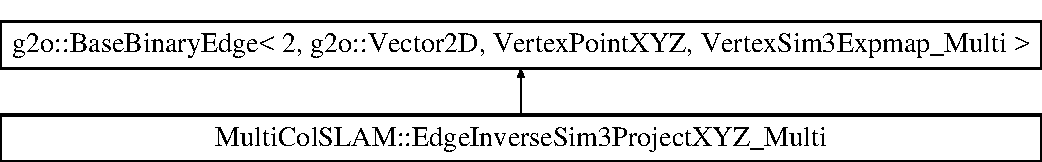
\includegraphics[height=2.000000cm]{classMultiColSLAM_1_1EdgeInverseSim3ProjectXYZ__Multi}
\end{center}
\end{figure}
\subsection*{Public Member Functions}
\begin{DoxyCompactItemize}
\item 
void {\bfseries compute\+Error} ()\hypertarget{classMultiColSLAM_1_1EdgeInverseSim3ProjectXYZ__Multi_ad2c7dfc67867f217aca806fd9a2a6cd7}{}\label{classMultiColSLAM_1_1EdgeInverseSim3ProjectXYZ__Multi_ad2c7dfc67867f217aca806fd9a2a6cd7}

\item 
bool {\bfseries read} (std\+::istream \&is)\hypertarget{classMultiColSLAM_1_1EdgeInverseSim3ProjectXYZ__Multi_ad1f8040a1e204d6c8ab18fd91aae928d}{}\label{classMultiColSLAM_1_1EdgeInverseSim3ProjectXYZ__Multi_ad1f8040a1e204d6c8ab18fd91aae928d}

\item 
bool {\bfseries write} (std\+::ostream \&os) const \hypertarget{classMultiColSLAM_1_1EdgeInverseSim3ProjectXYZ__Multi_a9f7d94af5867926b3d16ef5152d5d246}{}\label{classMultiColSLAM_1_1EdgeInverseSim3ProjectXYZ__Multi_a9f7d94af5867926b3d16ef5152d5d246}

\end{DoxyCompactItemize}


The documentation for this class was generated from the following file\+:\begin{DoxyCompactItemize}
\item 
include/g2o\+\_\+\+Multi\+Col\+\_\+sim3\+\_\+expmap.\+h\end{DoxyCompactItemize}

\hypertarget{classMultiColSLAM_1_1EdgeProjectXYZ2MCS}{}\section{Multi\+Col\+S\+L\+AM\+:\+:Edge\+Project\+X\+Y\+Z2\+M\+CS Class Reference}
\label{classMultiColSLAM_1_1EdgeProjectXYZ2MCS}\index{Multi\+Col\+S\+L\+A\+M\+::\+Edge\+Project\+X\+Y\+Z2\+M\+CS@{Multi\+Col\+S\+L\+A\+M\+::\+Edge\+Project\+X\+Y\+Z2\+M\+CS}}
Inheritance diagram for Multi\+Col\+S\+L\+AM\+:\+:Edge\+Project\+X\+Y\+Z2\+M\+CS\+:\begin{figure}[H]
\begin{center}
\leavevmode
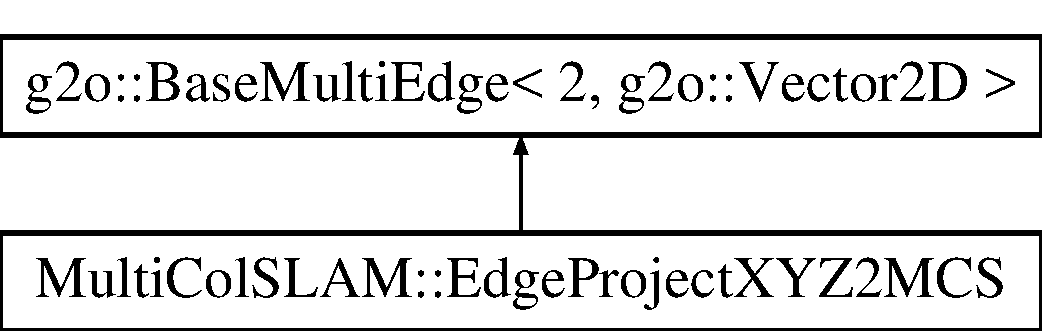
\includegraphics[height=2.000000cm]{classMultiColSLAM_1_1EdgeProjectXYZ2MCS}
\end{center}
\end{figure}
\subsection*{Public Member Functions}
\begin{DoxyCompactItemize}
\item 
virtual bool {\bfseries read} (std\+::istream \&)\hypertarget{classMultiColSLAM_1_1EdgeProjectXYZ2MCS_a3209ed8727aacd154af127e459f46cf8}{}\label{classMultiColSLAM_1_1EdgeProjectXYZ2MCS_a3209ed8727aacd154af127e459f46cf8}

\item 
virtual bool {\bfseries write} (std\+::ostream \&) const \hypertarget{classMultiColSLAM_1_1EdgeProjectXYZ2MCS_a8c7d9e00cbfdb3afddf35d2280e82e67}{}\label{classMultiColSLAM_1_1EdgeProjectXYZ2MCS_a8c7d9e00cbfdb3afddf35d2280e82e67}

\item 
void {\bfseries compute\+Error} ()\hypertarget{classMultiColSLAM_1_1EdgeProjectXYZ2MCS_a5f7748e82b07f9d8b26f9583300276b5}{}\label{classMultiColSLAM_1_1EdgeProjectXYZ2MCS_a5f7748e82b07f9d8b26f9583300276b5}

\item 
void {\bfseries linearize\+Oplus} ()\hypertarget{classMultiColSLAM_1_1EdgeProjectXYZ2MCS_aea66f5096425d15763c1409876915625}{}\label{classMultiColSLAM_1_1EdgeProjectXYZ2MCS_aea66f5096425d15763c1409876915625}

\end{DoxyCompactItemize}


The documentation for this class was generated from the following file\+:\begin{DoxyCompactItemize}
\item 
include/g2o\+\_\+\+Multi\+Col\+\_\+vertices\+\_\+edges.\+h\end{DoxyCompactItemize}

\hypertarget{classMultiColSLAM_1_1edgeSim3}{}\section{Multi\+Col\+S\+L\+AM\+:\+:edge\+Sim3 Class Reference}
\label{classMultiColSLAM_1_1edgeSim3}\index{Multi\+Col\+S\+L\+A\+M\+::edge\+Sim3@{Multi\+Col\+S\+L\+A\+M\+::edge\+Sim3}}


7D edge between two Vertex7  




{\ttfamily \#include $<$g2o\+\_\+\+Multi\+Col\+\_\+sim3\+\_\+expmap.\+h$>$}

Inheritance diagram for Multi\+Col\+S\+L\+AM\+:\+:edge\+Sim3\+:\begin{figure}[H]
\begin{center}
\leavevmode
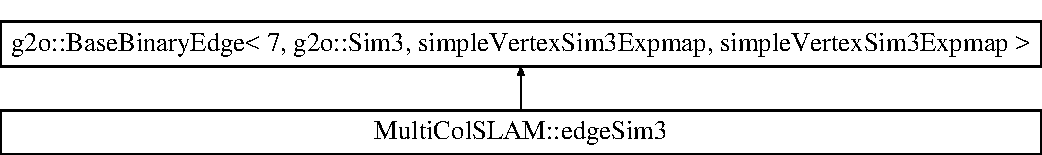
\includegraphics[height=2.000000cm]{classMultiColSLAM_1_1edgeSim3}
\end{center}
\end{figure}
\subsection*{Public Member Functions}
\begin{DoxyCompactItemize}
\item 
virtual bool {\bfseries read} (std\+::istream \&is)\hypertarget{classMultiColSLAM_1_1edgeSim3_a6d0a00d574e2790489dd7e339eea6e14}{}\label{classMultiColSLAM_1_1edgeSim3_a6d0a00d574e2790489dd7e339eea6e14}

\item 
virtual bool {\bfseries write} (std\+::ostream \&os) const \hypertarget{classMultiColSLAM_1_1edgeSim3_ae78172a053808aecbea596c90d199b13}{}\label{classMultiColSLAM_1_1edgeSim3_ae78172a053808aecbea596c90d199b13}

\item 
void {\bfseries compute\+Error} ()\hypertarget{classMultiColSLAM_1_1edgeSim3_a3109ef0d6e822daa23e3626234d75238}{}\label{classMultiColSLAM_1_1edgeSim3_a3109ef0d6e822daa23e3626234d75238}

\item 
virtual double {\bfseries initial\+Estimate\+Possible} (const g2o\+::\+Optimizable\+Graph\+::\+Vertex\+Set \&, g2o\+::\+Optimizable\+Graph\+::\+Vertex $\ast$)\hypertarget{classMultiColSLAM_1_1edgeSim3_a52be452ec95d32092c3c2ccea82dd4d0}{}\label{classMultiColSLAM_1_1edgeSim3_a52be452ec95d32092c3c2ccea82dd4d0}

\item 
virtual void {\bfseries initial\+Estimate} (const g2o\+::\+Optimizable\+Graph\+::\+Vertex\+Set \&from, g2o\+::\+Optimizable\+Graph\+::\+Vertex $\ast$)\hypertarget{classMultiColSLAM_1_1edgeSim3_a51b1391315d26872608b3cc215b25960}{}\label{classMultiColSLAM_1_1edgeSim3_a51b1391315d26872608b3cc215b25960}

\end{DoxyCompactItemize}


\subsection{Detailed Description}
7D edge between two Vertex7 

The documentation for this class was generated from the following file\+:\begin{DoxyCompactItemize}
\item 
include/g2o\+\_\+\+Multi\+Col\+\_\+sim3\+\_\+expmap.\+h\end{DoxyCompactItemize}

\hypertarget{classMultiColSLAM_1_1EdgeSim3__Multi}{}\section{Multi\+Col\+S\+L\+AM\+:\+:Edge\+Sim3\+\_\+\+Multi Class Reference}
\label{classMultiColSLAM_1_1EdgeSim3__Multi}\index{Multi\+Col\+S\+L\+A\+M\+::\+Edge\+Sim3\+\_\+\+Multi@{Multi\+Col\+S\+L\+A\+M\+::\+Edge\+Sim3\+\_\+\+Multi}}


7D edge between two Vertex7  




{\ttfamily \#include $<$g2o\+\_\+\+Multi\+Col\+\_\+sim3\+\_\+expmap.\+h$>$}

Inheritance diagram for Multi\+Col\+S\+L\+AM\+:\+:Edge\+Sim3\+\_\+\+Multi\+:\begin{figure}[H]
\begin{center}
\leavevmode
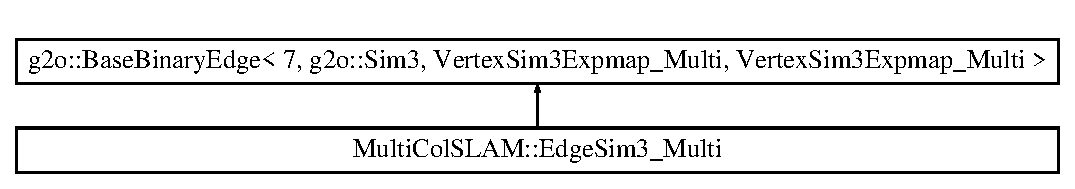
\includegraphics[height=2.000000cm]{classMultiColSLAM_1_1EdgeSim3__Multi}
\end{center}
\end{figure}
\subsection*{Public Member Functions}
\begin{DoxyCompactItemize}
\item 
void {\bfseries compute\+Error} ()\hypertarget{classMultiColSLAM_1_1EdgeSim3__Multi_aff9595501c9848f7c94de92146723abb}{}\label{classMultiColSLAM_1_1EdgeSim3__Multi_aff9595501c9848f7c94de92146723abb}

\item 
virtual double {\bfseries initial\+Estimate\+Possible} (const g2o\+::\+Optimizable\+Graph\+::\+Vertex\+Set \&, g2o\+::\+Optimizable\+Graph\+::\+Vertex $\ast$)\hypertarget{classMultiColSLAM_1_1EdgeSim3__Multi_a84ca699f4b20eaa9b1c284dee3fde36e}{}\label{classMultiColSLAM_1_1EdgeSim3__Multi_a84ca699f4b20eaa9b1c284dee3fde36e}

\item 
virtual void {\bfseries initial\+Estimate} (const g2o\+::\+Optimizable\+Graph\+::\+Vertex\+Set \&from, g2o\+::\+Optimizable\+Graph\+::\+Vertex $\ast$)\hypertarget{classMultiColSLAM_1_1EdgeSim3__Multi_af0e904350e4b73ea998a8372d8e96579}{}\label{classMultiColSLAM_1_1EdgeSim3__Multi_af0e904350e4b73ea998a8372d8e96579}

\item 
bool {\bfseries read} (std\+::istream \&is)\hypertarget{classMultiColSLAM_1_1EdgeSim3__Multi_a3172ba87b4a6c70e00a8c004e43ef4ac}{}\label{classMultiColSLAM_1_1EdgeSim3__Multi_a3172ba87b4a6c70e00a8c004e43ef4ac}

\item 
bool {\bfseries write} (std\+::ostream \&os) const \hypertarget{classMultiColSLAM_1_1EdgeSim3__Multi_afb9777e092f7aaf9f72d722c262eac6d}{}\label{classMultiColSLAM_1_1EdgeSim3__Multi_afb9777e092f7aaf9f72d722c262eac6d}

\end{DoxyCompactItemize}


\subsection{Detailed Description}
7D edge between two Vertex7 

The documentation for this class was generated from the following file\+:\begin{DoxyCompactItemize}
\item 
include/g2o\+\_\+\+Multi\+Col\+\_\+sim3\+\_\+expmap.\+h\end{DoxyCompactItemize}

\hypertarget{classMultiColSLAM_1_1EdgeSim3ProjectXYZ__Multi}{}\section{Multi\+Col\+S\+L\+AM\+:\+:Edge\+Sim3\+Project\+X\+Y\+Z\+\_\+\+Multi Class Reference}
\label{classMultiColSLAM_1_1EdgeSim3ProjectXYZ__Multi}\index{Multi\+Col\+S\+L\+A\+M\+::\+Edge\+Sim3\+Project\+X\+Y\+Z\+\_\+\+Multi@{Multi\+Col\+S\+L\+A\+M\+::\+Edge\+Sim3\+Project\+X\+Y\+Z\+\_\+\+Multi}}
Inheritance diagram for Multi\+Col\+S\+L\+AM\+:\+:Edge\+Sim3\+Project\+X\+Y\+Z\+\_\+\+Multi\+:\begin{figure}[H]
\begin{center}
\leavevmode
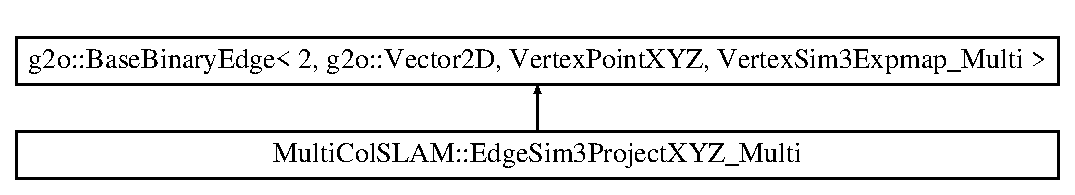
\includegraphics[height=2.000000cm]{classMultiColSLAM_1_1EdgeSim3ProjectXYZ__Multi}
\end{center}
\end{figure}
\subsection*{Public Member Functions}
\begin{DoxyCompactItemize}
\item 
void {\bfseries compute\+Error} ()\hypertarget{classMultiColSLAM_1_1EdgeSim3ProjectXYZ__Multi_a3fd027e5a2eef9364d1f5e75ab3fe1f2}{}\label{classMultiColSLAM_1_1EdgeSim3ProjectXYZ__Multi_a3fd027e5a2eef9364d1f5e75ab3fe1f2}

\item 
bool {\bfseries read} (std\+::istream \&is)\hypertarget{classMultiColSLAM_1_1EdgeSim3ProjectXYZ__Multi_aae98a41d1bebf78e191b1603ce896926}{}\label{classMultiColSLAM_1_1EdgeSim3ProjectXYZ__Multi_aae98a41d1bebf78e191b1603ce896926}

\item 
bool {\bfseries write} (std\+::ostream \&os) const \hypertarget{classMultiColSLAM_1_1EdgeSim3ProjectXYZ__Multi_ac91372b0ac8383263aa6a86f684e61ca}{}\label{classMultiColSLAM_1_1EdgeSim3ProjectXYZ__Multi_ac91372b0ac8383263aa6a86f684e61ca}

\end{DoxyCompactItemize}


The documentation for this class was generated from the following file\+:\begin{DoxyCompactItemize}
\item 
include/g2o\+\_\+\+Multi\+Col\+\_\+sim3\+\_\+expmap.\+h\end{DoxyCompactItemize}

\hypertarget{classExtractorNode}{}\section{Extractor\+Node Class Reference}
\label{classExtractorNode}\index{Extractor\+Node@{Extractor\+Node}}


{\ttfamily \#include $<$c\+O\+R\+Bextractor.\+h$>$}

\subsection*{Public Member Functions}
\begin{DoxyCompactItemize}
\item 
void {\bfseries Divide\+Node} (\hyperlink{classExtractorNode}{Extractor\+Node} \&n1, \hyperlink{classExtractorNode}{Extractor\+Node} \&n2, \hyperlink{classExtractorNode}{Extractor\+Node} \&n3, \hyperlink{classExtractorNode}{Extractor\+Node} \&n4)\hypertarget{classExtractorNode_acc0f41f35ca9077598fbdfa189fa1b98}{}\label{classExtractorNode_acc0f41f35ca9077598fbdfa189fa1b98}

\end{DoxyCompactItemize}
\subsection*{Public Attributes}
\begin{DoxyCompactItemize}
\item 
std\+::vector$<$ cv\+::\+Key\+Point $>$ {\bfseries v\+Keys}\hypertarget{classExtractorNode_a0fe322bb6db10c5d07656faddaecc59c}{}\label{classExtractorNode_a0fe322bb6db10c5d07656faddaecc59c}

\item 
cv\+::\+Point2i {\bfseries UL}\hypertarget{classExtractorNode_a5db748571d638f158feb52eb7184948b}{}\label{classExtractorNode_a5db748571d638f158feb52eb7184948b}

\item 
cv\+::\+Point2i {\bfseries UR}\hypertarget{classExtractorNode_ac4dbe288b3a8f43d7cba6022e030141b}{}\label{classExtractorNode_ac4dbe288b3a8f43d7cba6022e030141b}

\item 
cv\+::\+Point2i {\bfseries BL}\hypertarget{classExtractorNode_a579f50e7f9328c2f59c3b82294466a4d}{}\label{classExtractorNode_a579f50e7f9328c2f59c3b82294466a4d}

\item 
cv\+::\+Point2i {\bfseries BR}\hypertarget{classExtractorNode_acd1ba8d6c9fa83c768e52cfec285a551}{}\label{classExtractorNode_acd1ba8d6c9fa83c768e52cfec285a551}

\item 
std\+::list$<$ \hyperlink{classExtractorNode}{Extractor\+Node} $>$\+::iterator {\bfseries lit}\hypertarget{classExtractorNode_af12511d691299cdb53df0eb8d44afd3e}{}\label{classExtractorNode_af12511d691299cdb53df0eb8d44afd3e}

\item 
bool {\bfseries b\+No\+More}\hypertarget{classExtractorNode_a70dc749f6bc81a0ff4085e36eb61ed3b}{}\label{classExtractorNode_a70dc749f6bc81a0ff4085e36eb61ed3b}

\end{DoxyCompactItemize}


\subsection{Detailed Description}
This file is part of O\+R\+B-\/\+S\+L\+AM.

Copyright (C) 2014 Raúl Mur-\/\+Artal $<$raulmur at=\char`\"{}\char`\"{} unizar=\char`\"{}\char`\"{} dot=\char`\"{}\char`\"{} es$>$=\char`\"{}\char`\"{}$>$ (University of Zaragoza) For more information see \href{http://webdiis.unizar.es/~raulmur/orbslam/}{\tt http\+://webdiis.\+unizar.\+es/$\sim$raulmur/orbslam/}

O\+R\+B-\/\+S\+L\+AM is free software\+: you can redistribute it and/or modify it under the terms of the G\+NU General Public License as published by the Free Software Foundation, either version 3 of the License, or (at your option) any later version.

O\+R\+B-\/\+S\+L\+AM is distributed in the hope that it will be useful, but W\+I\+T\+H\+O\+UT A\+NY W\+A\+R\+R\+A\+N\+TY; without even the implied warranty of M\+E\+R\+C\+H\+A\+N\+T\+A\+B\+I\+L\+I\+TY or F\+I\+T\+N\+E\+SS F\+OR A P\+A\+R\+T\+I\+C\+U\+L\+AR P\+U\+R\+P\+O\+SE. See the G\+NU General Public License for more details.

You should have received a copy of the G\+NU General Public License along with O\+R\+B-\/\+S\+L\+AM. If not, see \href{http://www.gnu.org/licenses/}{\tt http\+://www.\+gnu.\+org/licenses/}. 

The documentation for this class was generated from the following file\+:\begin{DoxyCompactItemize}
\item 
include/c\+O\+R\+Bextractor.\+h\end{DoxyCompactItemize}

\hypertarget{classMultiColSLAM_1_1ExtractorNode__mdbrief}{}\section{Multi\+Col\+S\+L\+AM\+:\+:Extractor\+Node\+\_\+mdbrief Class Reference}
\label{classMultiColSLAM_1_1ExtractorNode__mdbrief}\index{Multi\+Col\+S\+L\+A\+M\+::\+Extractor\+Node\+\_\+mdbrief@{Multi\+Col\+S\+L\+A\+M\+::\+Extractor\+Node\+\_\+mdbrief}}
\subsection*{Public Member Functions}
\begin{DoxyCompactItemize}
\item 
void {\bfseries Divide\+Node} (\hyperlink{classMultiColSLAM_1_1ExtractorNode__mdbrief}{Extractor\+Node\+\_\+mdbrief} \&n1, \hyperlink{classMultiColSLAM_1_1ExtractorNode__mdbrief}{Extractor\+Node\+\_\+mdbrief} \&n2, \hyperlink{classMultiColSLAM_1_1ExtractorNode__mdbrief}{Extractor\+Node\+\_\+mdbrief} \&n3, \hyperlink{classMultiColSLAM_1_1ExtractorNode__mdbrief}{Extractor\+Node\+\_\+mdbrief} \&n4)\hypertarget{classMultiColSLAM_1_1ExtractorNode__mdbrief_a6980d601362ad9ea094bcdbb1884b04b}{}\label{classMultiColSLAM_1_1ExtractorNode__mdbrief_a6980d601362ad9ea094bcdbb1884b04b}

\end{DoxyCompactItemize}
\subsection*{Public Attributes}
\begin{DoxyCompactItemize}
\item 
std\+::vector$<$ cv\+::\+Key\+Point $>$ {\bfseries v\+Keys}\hypertarget{classMultiColSLAM_1_1ExtractorNode__mdbrief_aec88cb90c80aae9a73dfd9194d9cb7a4}{}\label{classMultiColSLAM_1_1ExtractorNode__mdbrief_aec88cb90c80aae9a73dfd9194d9cb7a4}

\item 
cv\+::\+Point2i {\bfseries UL}\hypertarget{classMultiColSLAM_1_1ExtractorNode__mdbrief_ae1685a789c125a7c3e6e7b822c08592d}{}\label{classMultiColSLAM_1_1ExtractorNode__mdbrief_ae1685a789c125a7c3e6e7b822c08592d}

\item 
cv\+::\+Point2i {\bfseries UR}\hypertarget{classMultiColSLAM_1_1ExtractorNode__mdbrief_a43e6ae76b64cb2a5e652ca38158a2fa4}{}\label{classMultiColSLAM_1_1ExtractorNode__mdbrief_a43e6ae76b64cb2a5e652ca38158a2fa4}

\item 
cv\+::\+Point2i {\bfseries BL}\hypertarget{classMultiColSLAM_1_1ExtractorNode__mdbrief_a21ee9ad0d775f15b76226ae08c0ef3b1}{}\label{classMultiColSLAM_1_1ExtractorNode__mdbrief_a21ee9ad0d775f15b76226ae08c0ef3b1}

\item 
cv\+::\+Point2i {\bfseries BR}\hypertarget{classMultiColSLAM_1_1ExtractorNode__mdbrief_a5cdd7deb1b7b1b5da128cb0fc72bb214}{}\label{classMultiColSLAM_1_1ExtractorNode__mdbrief_a5cdd7deb1b7b1b5da128cb0fc72bb214}

\item 
std\+::list$<$ \hyperlink{classMultiColSLAM_1_1ExtractorNode__mdbrief}{Extractor\+Node\+\_\+mdbrief} $>$\+::iterator {\bfseries lit}\hypertarget{classMultiColSLAM_1_1ExtractorNode__mdbrief_a5d989a8b7c1a91968db699eafbbc97a1}{}\label{classMultiColSLAM_1_1ExtractorNode__mdbrief_a5d989a8b7c1a91968db699eafbbc97a1}

\item 
bool {\bfseries b\+No\+More}\hypertarget{classMultiColSLAM_1_1ExtractorNode__mdbrief_a69042629292a1fd938f348d11e4976c6}{}\label{classMultiColSLAM_1_1ExtractorNode__mdbrief_a69042629292a1fd938f348d11e4976c6}

\end{DoxyCompactItemize}


The documentation for this class was generated from the following file\+:\begin{DoxyCompactItemize}
\item 
include/md\+B\+R\+I\+E\+Fextractor\+Oct.\+h\end{DoxyCompactItemize}

\hypertarget{classmdBRIEFextractor}{}\section{md\+B\+R\+I\+E\+Fextractor Class Reference}
\label{classmdBRIEFextractor}\index{md\+B\+R\+I\+E\+Fextractor@{md\+B\+R\+I\+E\+Fextractor}}
\subsection*{Public Types}
\begin{DoxyCompactItemize}
\item 
enum \{ {\bfseries H\+A\+R\+R\+I\+S\+\_\+\+S\+C\+O\+RE} =0, 
{\bfseries F\+A\+S\+T\+\_\+\+S\+C\+O\+RE} =1
 \}\hypertarget{classmdBRIEFextractor_a2279809ca1249b3020ac675e25d0a20d}{}\label{classmdBRIEFextractor_a2279809ca1249b3020ac675e25d0a20d}

\end{DoxyCompactItemize}
\subsection*{Public Member Functions}
\begin{DoxyCompactItemize}
\item 
{\bfseries md\+B\+R\+I\+E\+Fextractor} (int \+\_\+nfeatures=1000, float \+\_\+scale\+Factor=1.\+2, int \+\_\+nlevels=8, int \+\_\+edge\+Threshold=25, int \+\_\+first\+Level=0, int \+\_\+score\+Type=H\+A\+R\+R\+I\+S\+\_\+\+S\+C\+O\+RE, int \+\_\+patch\+Size=32, int \+\_\+fast\+Threshold=20, bool \+\_\+use\+Agast=false, int \+\_\+fast\+Agast\+Type=2, bool \+\_\+learn\+Masks=false, int \+\_\+desc\+Size=32)\hypertarget{classmdBRIEFextractor_aa27776bf46a0c9577c1b7cb996deea60}{}\label{classmdBRIEFextractor_aa27776bf46a0c9577c1b7cb996deea60}

\item 
void {\bfseries operator()} (cv\+::\+Input\+Array \+\_\+image, cv\+::\+Input\+Array \+\_\+mask, std\+::vector$<$ cv\+::\+Key\+Point $>$ \&\+\_\+keypoints, c\+Cam\+Model\+General\+\_\+ \&cam\+Model, cv\+::\+Output\+Array \+\_\+descriptors, cv\+::\+Output\+Array \+\_\+descriptor\+Masks)\hypertarget{classmdBRIEFextractor_a156d65fed08bcb31eafca1fb8f3ba2b7}{}\label{classmdBRIEFextractor_a156d65fed08bcb31eafca1fb8f3ba2b7}

\item 
int {\bfseries Get\+Levels} ()\hypertarget{classmdBRIEFextractor_a77a55b01f8c829bc5a402ed984a636ab}{}\label{classmdBRIEFextractor_a77a55b01f8c829bc5a402ed984a636ab}

\item 
double {\bfseries Get\+Scale\+Factor} ()\hypertarget{classmdBRIEFextractor_a2fc1fac3f793191e1e7de1b5b6c3062c}{}\label{classmdBRIEFextractor_a2fc1fac3f793191e1e7de1b5b6c3062c}

\item 
bool {\bfseries Get\+Masks\+Learned} ()\hypertarget{classmdBRIEFextractor_a0f0028be442cff90f0da8cf7956c0ee3}{}\label{classmdBRIEFextractor_a0f0028be442cff90f0da8cf7956c0ee3}

\item 
int {\bfseries Get\+Descriptor\+Size} ()\hypertarget{classmdBRIEFextractor_a6f343fc7ead5bb8714a483fad353e977}{}\label{classmdBRIEFextractor_a6f343fc7ead5bb8714a483fad353e977}

\end{DoxyCompactItemize}
\subsection*{Static Public Attributes}
\begin{DoxyCompactItemize}
\item 
static int {\bfseries H\+A\+L\+F\+\_\+\+P\+A\+T\+C\+H\+\_\+\+S\+I\+ZE}\hypertarget{classmdBRIEFextractor_aa4ff165effca9090aafbcc78172571bd}{}\label{classmdBRIEFextractor_aa4ff165effca9090aafbcc78172571bd}

\item 
static int {\bfseries E\+D\+G\+E\+\_\+\+T\+H\+R\+E\+S\+H\+O\+LD}\hypertarget{classmdBRIEFextractor_acca8f6f32082195ccb23acb6616cb67e}{}\label{classmdBRIEFextractor_acca8f6f32082195ccb23acb6616cb67e}

\end{DoxyCompactItemize}
\subsection*{Protected Member Functions}
\begin{DoxyCompactItemize}
\item 
int {\bfseries descriptor\+Size} () const \hypertarget{classmdBRIEFextractor_a9de61227e11bd3a79339197e7d68071c}{}\label{classmdBRIEFextractor_a9de61227e11bd3a79339197e7d68071c}

\item 
int {\bfseries descriptor\+Type} () const \hypertarget{classmdBRIEFextractor_adf35fa5de268c265694a3bfb1b1de41b}{}\label{classmdBRIEFextractor_adf35fa5de268c265694a3bfb1b1de41b}

\item 
int {\bfseries default\+Norm} () const \hypertarget{classmdBRIEFextractor_abbbcf3ddb0a8a9cf2e907495fb2dc688}{}\label{classmdBRIEFextractor_abbbcf3ddb0a8a9cf2e907495fb2dc688}

\item 
void {\bfseries Compute\+Pyramid} (cv\+::\+Mat image, cv\+::\+Mat Mask=cv\+::\+Mat())\hypertarget{classmdBRIEFextractor_a343fc2937c41686f0794c30b0d57e594}{}\label{classmdBRIEFextractor_a343fc2937c41686f0794c30b0d57e594}

\item 
void {\bfseries Compute\+Key\+Points} (std\+::vector$<$ std\+::vector$<$ cv\+::\+Key\+Point $>$ $>$ \&all\+Keypoints)\hypertarget{classmdBRIEFextractor_a286c01b9ff8c90f4ff3d704b66635f6a}{}\label{classmdBRIEFextractor_a286c01b9ff8c90f4ff3d704b66635f6a}

\end{DoxyCompactItemize}
\subsection*{Protected Attributes}
\begin{DoxyCompactItemize}
\item 
std\+::vector$<$ cv\+::\+Point $>$ {\bfseries pattern}\hypertarget{classmdBRIEFextractor_acf4203311d4a48cca2c4e01a6095fda9}{}\label{classmdBRIEFextractor_acf4203311d4a48cca2c4e01a6095fda9}

\item 
int {\bfseries nfeatures}\hypertarget{classmdBRIEFextractor_ad05427a45d8bb5b3e6eb629c4829a65b}{}\label{classmdBRIEFextractor_ad05427a45d8bb5b3e6eb629c4829a65b}

\item 
double {\bfseries scale\+Factor}\hypertarget{classmdBRIEFextractor_a68bd33089308f7d68081d3b1f36efae3}{}\label{classmdBRIEFextractor_a68bd33089308f7d68081d3b1f36efae3}

\item 
int {\bfseries numlevels}\hypertarget{classmdBRIEFextractor_ac80b0ccd907ca35f5096e707836eb499}{}\label{classmdBRIEFextractor_ac80b0ccd907ca35f5096e707836eb499}

\item 
int {\bfseries edge\+Threshold}\hypertarget{classmdBRIEFextractor_a4bf058ab2585da8d2fb4df9e1871bafb}{}\label{classmdBRIEFextractor_a4bf058ab2585da8d2fb4df9e1871bafb}

\item 
int {\bfseries first\+Level}\hypertarget{classmdBRIEFextractor_a92f484d3841fe88adc9f3f280377b53f}{}\label{classmdBRIEFextractor_a92f484d3841fe88adc9f3f280377b53f}

\item 
int {\bfseries desc\+Size}\hypertarget{classmdBRIEFextractor_a07096c62f2e2ba12966e92ddd455abdf}{}\label{classmdBRIEFextractor_a07096c62f2e2ba12966e92ddd455abdf}

\item 
int {\bfseries score\+Type}\hypertarget{classmdBRIEFextractor_a321a33a3ddc6037f61858c20cb10904f}{}\label{classmdBRIEFextractor_a321a33a3ddc6037f61858c20cb10904f}

\item 
int {\bfseries patch\+Size}\hypertarget{classmdBRIEFextractor_ad6b2cffb3a69691c306a20951a68e04a}{}\label{classmdBRIEFextractor_ad6b2cffb3a69691c306a20951a68e04a}

\item 
int {\bfseries fast\+Threshold}\hypertarget{classmdBRIEFextractor_a860fb0c609bd868175eb6a9704a0f644}{}\label{classmdBRIEFextractor_a860fb0c609bd868175eb6a9704a0f644}

\item 
bool {\bfseries use\+Agast}\hypertarget{classmdBRIEFextractor_a13804fd6cd95184e935c36fcea3bf19e}{}\label{classmdBRIEFextractor_a13804fd6cd95184e935c36fcea3bf19e}

\item 
int {\bfseries fast\+Agast\+Type}\hypertarget{classmdBRIEFextractor_affeccac13fe4a4981116a6d84f0759c3}{}\label{classmdBRIEFextractor_affeccac13fe4a4981116a6d84f0759c3}

\item 
bool {\bfseries learn\+Masks}\hypertarget{classmdBRIEFextractor_a2d879fa10c9b7798d47403d835890bb5}{}\label{classmdBRIEFextractor_a2d879fa10c9b7798d47403d835890bb5}

\item 
int {\bfseries half\+\_\+patch\+\_\+size}\hypertarget{classmdBRIEFextractor_a987a1f7a9beea23fe5eb3e6b731e70a2}{}\label{classmdBRIEFextractor_a987a1f7a9beea23fe5eb3e6b731e70a2}

\item 
std\+::vector$<$ int $>$ {\bfseries mn\+Features\+Per\+Level}\hypertarget{classmdBRIEFextractor_a25af3a314c66c461e893c9ade0a19d03}{}\label{classmdBRIEFextractor_a25af3a314c66c461e893c9ade0a19d03}

\item 
std\+::vector$<$ int $>$ {\bfseries umax}\hypertarget{classmdBRIEFextractor_aa491ccf730f1f2f9e69c800cb10f4f70}{}\label{classmdBRIEFextractor_aa491ccf730f1f2f9e69c800cb10f4f70}

\item 
std\+::vector$<$ double $>$ {\bfseries mv\+Scale\+Factor}\hypertarget{classmdBRIEFextractor_a090e0df687a8e2ee205c79cad9add39b}{}\label{classmdBRIEFextractor_a090e0df687a8e2ee205c79cad9add39b}

\item 
std\+::vector$<$ double $>$ {\bfseries mv\+Inv\+Scale\+Factor}\hypertarget{classmdBRIEFextractor_af8987cf35f38bc905262d2d8fc9619c0}{}\label{classmdBRIEFextractor_af8987cf35f38bc905262d2d8fc9619c0}

\item 
std\+::vector$<$ cv\+::\+Mat $>$ {\bfseries mv\+Image\+Pyramid}\hypertarget{classmdBRIEFextractor_ab1b14557a72b264db8da1298042acf95}{}\label{classmdBRIEFextractor_ab1b14557a72b264db8da1298042acf95}

\item 
std\+::vector$<$ cv\+::\+Mat $>$ {\bfseries mv\+Mask\+Pyramid}\hypertarget{classmdBRIEFextractor_a8973c00c2a0f709ade7ea3f0cfc86a6f}{}\label{classmdBRIEFextractor_a8973c00c2a0f709ade7ea3f0cfc86a6f}

\end{DoxyCompactItemize}


The documentation for this class was generated from the following file\+:\begin{DoxyCompactItemize}
\item 
include/md\+B\+R\+I\+E\+Fextractor.\+h\end{DoxyCompactItemize}

\hypertarget{classmdBRIEFextractor1}{}\section{md\+B\+R\+I\+E\+Fextractor1 Class Reference}
\label{classmdBRIEFextractor1}\index{md\+B\+R\+I\+E\+Fextractor1@{md\+B\+R\+I\+E\+Fextractor1}}
\subsection*{Public Types}
\begin{DoxyCompactItemize}
\item 
enum \{ {\bfseries H\+A\+R\+R\+I\+S\+\_\+\+S\+C\+O\+RE} =0, 
{\bfseries F\+A\+S\+T\+\_\+\+S\+C\+O\+RE} =1
 \}\hypertarget{classmdBRIEFextractor1_a65b82fbc66e46a5d5d2f59b9220a92f0}{}\label{classmdBRIEFextractor1_a65b82fbc66e46a5d5d2f59b9220a92f0}

\end{DoxyCompactItemize}
\subsection*{Public Member Functions}
\begin{DoxyCompactItemize}
\item 
{\bfseries md\+B\+R\+I\+E\+Fextractor1} (int \+\_\+nfeatures=1000, float \+\_\+scale\+Factor=1.\+2, int \+\_\+nlevels=8, int \+\_\+edge\+Threshold=25, int \+\_\+first\+Level=0, int \+\_\+score\+Type=H\+A\+R\+R\+I\+S\+\_\+\+S\+C\+O\+RE, int \+\_\+patch\+Size=32, int \+\_\+fast\+Threshold=20, bool \+\_\+use\+Agast=false, int \+\_\+fast\+Agast\+Type=2, bool \+\_\+learn\+Masks=false, int \+\_\+desc\+Size=32)\hypertarget{classmdBRIEFextractor1_a205bde79556596526ae791c050f21ee8}{}\label{classmdBRIEFextractor1_a205bde79556596526ae791c050f21ee8}

\item 
void {\bfseries detect\+And\+Compute} (cv\+::\+Input\+Array image, cv\+::\+Input\+Array mask, std\+::vector$<$ cv\+::\+Key\+Point $>$ \&keypoints, cv\+::\+Output\+Array descriptors, cv\+::\+Output\+Array descriptor\+Masks, c\+Cam\+Model\+General\+\_\+ \&cam\+Model, bool use\+Provided\+Keypoints=false)\hypertarget{classmdBRIEFextractor1_aee118fb7a56b181f95be06a076d3a0fb}{}\label{classmdBRIEFextractor1_aee118fb7a56b181f95be06a076d3a0fb}

\item 
void {\bfseries compute} (cv\+::\+Input\+Array \+\_\+image, cv\+::\+Input\+Array \+\_\+mask, const std\+::vector$<$ cv\+::\+Key\+Point $>$ \&keypoints, const std\+::vector$<$ cv\+::\+Vec2f $>$ \&undist\+\_\+keypoints, cv\+::\+Output\+Array \+\_\+descriptors, cv\+::\+Output\+Array \+\_\+descriptor\+Masks, c\+Cam\+Model\+General\+\_\+ \&cam\+Model)\hypertarget{classmdBRIEFextractor1_ab76fa04826ab8276c668d8cb8dea68a5}{}\label{classmdBRIEFextractor1_ab76fa04826ab8276c668d8cb8dea68a5}

\item 
void {\bfseries detect} (cv\+::\+Input\+Array \+\_\+image, cv\+::\+Input\+Array \+\_\+mask, c\+Cam\+Model\+General\+\_\+ \&cam\+Model, std\+::vector$<$ cv\+::\+Key\+Point $>$ \&keypoints, std\+::vector$<$ cv\+::\+Vec2f $>$ \&undist\+\_\+keypoints)\hypertarget{classmdBRIEFextractor1_add5de740eca42464aa7e6a045f0407cc}{}\label{classmdBRIEFextractor1_add5de740eca42464aa7e6a045f0407cc}

\item 
int {\bfseries Get\+Levels} ()\hypertarget{classmdBRIEFextractor1_aef1fb456c93c569eab3d7bd5fb2e6517}{}\label{classmdBRIEFextractor1_aef1fb456c93c569eab3d7bd5fb2e6517}

\item 
double {\bfseries Get\+Scale\+Factor} ()\hypertarget{classmdBRIEFextractor1_a5f35126b7400d7bee0e2f985ddcb8efe}{}\label{classmdBRIEFextractor1_a5f35126b7400d7bee0e2f985ddcb8efe}

\item 
bool {\bfseries Get\+Masks\+Learned} ()\hypertarget{classmdBRIEFextractor1_aad00a30f095078c45a3f9f53c4c172ee}{}\label{classmdBRIEFextractor1_aad00a30f095078c45a3f9f53c4c172ee}

\item 
int {\bfseries Get\+Descriptor\+Size} ()\hypertarget{classmdBRIEFextractor1_aadcb14bcbb38f66deb2f74fd7f53c1ba}{}\label{classmdBRIEFextractor1_aadcb14bcbb38f66deb2f74fd7f53c1ba}

\end{DoxyCompactItemize}
\subsection*{Protected Member Functions}
\begin{DoxyCompactItemize}
\item 
int {\bfseries descriptor\+Size} () const \hypertarget{classmdBRIEFextractor1_a1bc510192ddb4a0ea8e4a31a3fa15676}{}\label{classmdBRIEFextractor1_a1bc510192ddb4a0ea8e4a31a3fa15676}

\item 
int {\bfseries descriptor\+Type} () const \hypertarget{classmdBRIEFextractor1_a50ce882363a537bb56ffcc7ad002b01b}{}\label{classmdBRIEFextractor1_a50ce882363a537bb56ffcc7ad002b01b}

\item 
int {\bfseries default\+Norm} () const \hypertarget{classmdBRIEFextractor1_ad1bad790d5775354793982e9146fb6f7}{}\label{classmdBRIEFextractor1_ad1bad790d5775354793982e9146fb6f7}

\end{DoxyCompactItemize}
\subsection*{Protected Attributes}
\begin{DoxyCompactItemize}
\item 
std\+::vector$<$ cv\+::\+Point $>$ {\bfseries pattern}\hypertarget{classmdBRIEFextractor1_a773e921ecc494358c403ba77ab4f2c0d}{}\label{classmdBRIEFextractor1_a773e921ecc494358c403ba77ab4f2c0d}

\item 
int {\bfseries nfeatures}\hypertarget{classmdBRIEFextractor1_ab8df4e7b45edbbdd6cb944788b1d835c}{}\label{classmdBRIEFextractor1_ab8df4e7b45edbbdd6cb944788b1d835c}

\item 
double {\bfseries scale\+Factor}\hypertarget{classmdBRIEFextractor1_a786dd5bb702802c48379630b73e0a7f7}{}\label{classmdBRIEFextractor1_a786dd5bb702802c48379630b73e0a7f7}

\item 
int {\bfseries numlevels}\hypertarget{classmdBRIEFextractor1_a162a334993065d291b7ad8a8b13457b5}{}\label{classmdBRIEFextractor1_a162a334993065d291b7ad8a8b13457b5}

\item 
int {\bfseries edge\+Threshold}\hypertarget{classmdBRIEFextractor1_a94775c3078ed208734b3535bc9e4af6a}{}\label{classmdBRIEFextractor1_a94775c3078ed208734b3535bc9e4af6a}

\item 
int {\bfseries first\+Level}\hypertarget{classmdBRIEFextractor1_a3e3a9d01780c4247dc810fede77be490}{}\label{classmdBRIEFextractor1_a3e3a9d01780c4247dc810fede77be490}

\item 
int {\bfseries desc\+Size}\hypertarget{classmdBRIEFextractor1_a52bbb0802c56cbaed48526cc1f42f5c3}{}\label{classmdBRIEFextractor1_a52bbb0802c56cbaed48526cc1f42f5c3}

\item 
int {\bfseries score\+Type}\hypertarget{classmdBRIEFextractor1_af7c1919fde3ba228734a1d6ea131bf4e}{}\label{classmdBRIEFextractor1_af7c1919fde3ba228734a1d6ea131bf4e}

\item 
int {\bfseries patch\+Size}\hypertarget{classmdBRIEFextractor1_a3383813982facadfc5452e8f3f2d55d0}{}\label{classmdBRIEFextractor1_a3383813982facadfc5452e8f3f2d55d0}

\item 
int {\bfseries fast\+Threshold}\hypertarget{classmdBRIEFextractor1_a917ed4eecd99e2ccfad6fb1fdb5fb2c9}{}\label{classmdBRIEFextractor1_a917ed4eecd99e2ccfad6fb1fdb5fb2c9}

\item 
bool {\bfseries use\+Agast}\hypertarget{classmdBRIEFextractor1_a302438233985316d3339955def3e120c}{}\label{classmdBRIEFextractor1_a302438233985316d3339955def3e120c}

\item 
int {\bfseries fast\+Agast\+Type}\hypertarget{classmdBRIEFextractor1_af8746fcd77fd7f41f10f5390f68d87d7}{}\label{classmdBRIEFextractor1_af8746fcd77fd7f41f10f5390f68d87d7}

\item 
bool {\bfseries learn\+Masks}\hypertarget{classmdBRIEFextractor1_a7acde3d9af442364327ff8a9b64c8374}{}\label{classmdBRIEFextractor1_a7acde3d9af442364327ff8a9b64c8374}

\item 
std\+::vector$<$ int $>$ {\bfseries mn\+Features\+Per\+Level}\hypertarget{classmdBRIEFextractor1_a12ab5edd862ba20eca826f402184acce}{}\label{classmdBRIEFextractor1_a12ab5edd862ba20eca826f402184acce}

\item 
std\+::vector$<$ int $>$ {\bfseries umax}\hypertarget{classmdBRIEFextractor1_ae796c51d02cc2dbcf37c142b6876ba53}{}\label{classmdBRIEFextractor1_ae796c51d02cc2dbcf37c142b6876ba53}

\item 
std\+::vector$<$ double $>$ {\bfseries mv\+Scale\+Factor}\hypertarget{classmdBRIEFextractor1_a6ecaa899738234ab1958bbd2506ee254}{}\label{classmdBRIEFextractor1_a6ecaa899738234ab1958bbd2506ee254}

\item 
std\+::vector$<$ double $>$ {\bfseries mv\+Inv\+Scale\+Factor}\hypertarget{classmdBRIEFextractor1_a82bcbbd1bd8c182a7f74460efe1afec4}{}\label{classmdBRIEFextractor1_a82bcbbd1bd8c182a7f74460efe1afec4}

\item 
std\+::vector$<$ cv\+::\+Mat $>$ {\bfseries mv\+Image\+Pyramid}\hypertarget{classmdBRIEFextractor1_a8b540b42ad288eb16788210a095907af}{}\label{classmdBRIEFextractor1_a8b540b42ad288eb16788210a095907af}

\item 
std\+::vector$<$ cv\+::\+Mat $>$ {\bfseries mv\+Mask\+Pyramid}\hypertarget{classmdBRIEFextractor1_ac44c6de3cee6625beb5125a85db829f4}{}\label{classmdBRIEFextractor1_ac44c6de3cee6625beb5125a85db829f4}

\end{DoxyCompactItemize}


The documentation for this class was generated from the following file\+:\begin{DoxyCompactItemize}
\item 
include/md\+B\+R\+I\+E\+Fextractor1.\+h\end{DoxyCompactItemize}

\hypertarget{classMultiColSLAM_1_1mdBRIEFextractorOct}{}\section{Multi\+Col\+S\+L\+AM\+:\+:md\+B\+R\+I\+E\+Fextractor\+Oct Class Reference}
\label{classMultiColSLAM_1_1mdBRIEFextractorOct}\index{Multi\+Col\+S\+L\+A\+M\+::md\+B\+R\+I\+E\+Fextractor\+Oct@{Multi\+Col\+S\+L\+A\+M\+::md\+B\+R\+I\+E\+Fextractor\+Oct}}
\subsection*{Public Types}
\begin{DoxyCompactItemize}
\item 
enum \{ {\bfseries H\+A\+R\+R\+I\+S\+\_\+\+S\+C\+O\+RE} = 0, 
{\bfseries F\+A\+S\+T\+\_\+\+S\+C\+O\+RE} = 1
 \}\hypertarget{classMultiColSLAM_1_1mdBRIEFextractorOct_a735244f6047412b75ac43a5d67f4c621}{}\label{classMultiColSLAM_1_1mdBRIEFextractorOct_a735244f6047412b75ac43a5d67f4c621}

\end{DoxyCompactItemize}
\subsection*{Public Member Functions}
\begin{DoxyCompactItemize}
\item 
{\bfseries md\+B\+R\+I\+E\+Fextractor\+Oct} (int \+\_\+nfeatures=1000, float \+\_\+scale\+Factor=1.\+2, int \+\_\+nlevels=8, int \+\_\+edge\+Threshold=25, int \+\_\+first\+Level=0, int \+\_\+score\+Type=H\+A\+R\+R\+I\+S\+\_\+\+S\+C\+O\+RE, int \+\_\+patch\+Size=32, int \+\_\+fast\+Threshold=20, bool \+\_\+use\+Agast=false, int \+\_\+fast\+Agast\+Type=2, bool \+\_\+do\+\_\+d\+Brief=false, bool \+\_\+learn\+Masks=false, int \+\_\+desc\+Size=32)\hypertarget{classMultiColSLAM_1_1mdBRIEFextractorOct_a97fcc207bd3003b907ab1215afa5456d}{}\label{classMultiColSLAM_1_1mdBRIEFextractorOct_a97fcc207bd3003b907ab1215afa5456d}

\item 
void {\bfseries operator()} (cv\+::\+Input\+Array \+\_\+image, cv\+::\+Input\+Array \+\_\+mask, std\+::vector$<$ cv\+::\+Key\+Point $>$ \&\+\_\+keypoints, \hyperlink{classMultiColSLAM_1_1cCamModelGeneral__}{c\+Cam\+Model\+General\+\_\+} \&cam\+Model, cv\+::\+Output\+Array \+\_\+descriptors, cv\+::\+Output\+Array \+\_\+descriptor\+Masks)\hypertarget{classMultiColSLAM_1_1mdBRIEFextractorOct_a58b277ef92295a6093b770fe60fb2d9c}{}\label{classMultiColSLAM_1_1mdBRIEFextractorOct_a58b277ef92295a6093b770fe60fb2d9c}

\item 
int {\bfseries Get\+Levels} ()\hypertarget{classMultiColSLAM_1_1mdBRIEFextractorOct_a93c891bb1a8ae2f9575b13514fafa4c8}{}\label{classMultiColSLAM_1_1mdBRIEFextractorOct_a93c891bb1a8ae2f9575b13514fafa4c8}

\item 
double {\bfseries Get\+Scale\+Factor} ()\hypertarget{classMultiColSLAM_1_1mdBRIEFextractorOct_a657048e5277d37abd4a28b2ed13935bb}{}\label{classMultiColSLAM_1_1mdBRIEFextractorOct_a657048e5277d37abd4a28b2ed13935bb}

\item 
bool {\bfseries Get\+Masks\+Learned} ()\hypertarget{classMultiColSLAM_1_1mdBRIEFextractorOct_aec28f8f96ec4cef48e398fa9c79e26a8}{}\label{classMultiColSLAM_1_1mdBRIEFextractorOct_aec28f8f96ec4cef48e398fa9c79e26a8}

\item 
int {\bfseries Get\+Descriptor\+Size} ()\hypertarget{classMultiColSLAM_1_1mdBRIEFextractorOct_ac6604059484ce79a9e46d9f6219db9bc}{}\label{classMultiColSLAM_1_1mdBRIEFextractorOct_ac6604059484ce79a9e46d9f6219db9bc}

\end{DoxyCompactItemize}
\subsection*{Protected Member Functions}
\begin{DoxyCompactItemize}
\item 
void {\bfseries Compute\+Pyramid} (cv\+::\+Mat image, cv\+::\+Mat Mask=cv\+::\+Mat())\hypertarget{classMultiColSLAM_1_1mdBRIEFextractorOct_a34e617b89aad33b8baf5ff160fa1480d}{}\label{classMultiColSLAM_1_1mdBRIEFextractorOct_a34e617b89aad33b8baf5ff160fa1480d}

\item 
void {\bfseries Compute\+Key\+Points\+Oct\+Tree} (std\+::vector$<$ std\+::vector$<$ cv\+::\+Key\+Point $>$ $>$ \&all\+Keypoints)\hypertarget{classMultiColSLAM_1_1mdBRIEFextractorOct_abc83299607474e76f195f47fafc97e64}{}\label{classMultiColSLAM_1_1mdBRIEFextractorOct_abc83299607474e76f195f47fafc97e64}

\item 
std\+::vector$<$ cv\+::\+Key\+Point $>$ {\bfseries Distribute\+Oct\+Tree} (const std\+::vector$<$ cv\+::\+Key\+Point $>$ \&v\+To\+Distribute\+Keys, const int \&minX, const int \&maxX, const int \&minY, const int \&maxY, const int \&n\+Features, const int \&level)\hypertarget{classMultiColSLAM_1_1mdBRIEFextractorOct_ad4bb778d8f3d9ff53cd1773fe1bcf915}{}\label{classMultiColSLAM_1_1mdBRIEFextractorOct_ad4bb778d8f3d9ff53cd1773fe1bcf915}

\item 
void {\bfseries Compute\+Key\+Points\+Old} (std\+::vector$<$ std\+::vector$<$ cv\+::\+Key\+Point $>$ $>$ \&all\+Keypoints)\hypertarget{classMultiColSLAM_1_1mdBRIEFextractorOct_ae56e6b739363fd3a80470eac6b229e59}{}\label{classMultiColSLAM_1_1mdBRIEFextractorOct_ae56e6b739363fd3a80470eac6b229e59}

\item 
int {\bfseries descriptor\+Size} () const \hypertarget{classMultiColSLAM_1_1mdBRIEFextractorOct_ae9dc926bc5cd772ed717b8892be1545d}{}\label{classMultiColSLAM_1_1mdBRIEFextractorOct_ae9dc926bc5cd772ed717b8892be1545d}

\item 
int {\bfseries descriptor\+Type} () const \hypertarget{classMultiColSLAM_1_1mdBRIEFextractorOct_ab87af935830b78d836cc1e44dc039d8b}{}\label{classMultiColSLAM_1_1mdBRIEFextractorOct_ab87af935830b78d836cc1e44dc039d8b}

\item 
int {\bfseries default\+Norm} () const \hypertarget{classMultiColSLAM_1_1mdBRIEFextractorOct_a9a1000e9964ef88b31941a9daf3e15f9}{}\label{classMultiColSLAM_1_1mdBRIEFextractorOct_a9a1000e9964ef88b31941a9daf3e15f9}

\end{DoxyCompactItemize}
\subsection*{Protected Attributes}
\begin{DoxyCompactItemize}
\item 
std\+::vector$<$ cv\+::\+Point $>$ {\bfseries pattern}\hypertarget{classMultiColSLAM_1_1mdBRIEFextractorOct_a5214f07df30c6a777b9df23d80f8383e}{}\label{classMultiColSLAM_1_1mdBRIEFextractorOct_a5214f07df30c6a777b9df23d80f8383e}

\item 
int {\bfseries nfeatures}\hypertarget{classMultiColSLAM_1_1mdBRIEFextractorOct_a599f92cb2511b765f9b1796843280650}{}\label{classMultiColSLAM_1_1mdBRIEFextractorOct_a599f92cb2511b765f9b1796843280650}

\item 
double {\bfseries scale\+Factor}\hypertarget{classMultiColSLAM_1_1mdBRIEFextractorOct_a716076eea98eacac500a36b4bf696b46}{}\label{classMultiColSLAM_1_1mdBRIEFextractorOct_a716076eea98eacac500a36b4bf696b46}

\item 
int {\bfseries numlevels}\hypertarget{classMultiColSLAM_1_1mdBRIEFextractorOct_ae7be0b4d39f2b81e776bf7fecaa543cb}{}\label{classMultiColSLAM_1_1mdBRIEFextractorOct_ae7be0b4d39f2b81e776bf7fecaa543cb}

\item 
int {\bfseries edge\+Threshold}\hypertarget{classMultiColSLAM_1_1mdBRIEFextractorOct_a558500d5584b5c4d642987bda3654e56}{}\label{classMultiColSLAM_1_1mdBRIEFextractorOct_a558500d5584b5c4d642987bda3654e56}

\item 
int {\bfseries first\+Level}\hypertarget{classMultiColSLAM_1_1mdBRIEFextractorOct_a007668632ce60e3071241462c8fb29e5}{}\label{classMultiColSLAM_1_1mdBRIEFextractorOct_a007668632ce60e3071241462c8fb29e5}

\item 
int {\bfseries desc\+Size}\hypertarget{classMultiColSLAM_1_1mdBRIEFextractorOct_a750901630e7a94551bd92563ddb9a30b}{}\label{classMultiColSLAM_1_1mdBRIEFextractorOct_a750901630e7a94551bd92563ddb9a30b}

\item 
int {\bfseries score\+Type}\hypertarget{classMultiColSLAM_1_1mdBRIEFextractorOct_af3f0c8c3531de98e77a03e345b5845a7}{}\label{classMultiColSLAM_1_1mdBRIEFextractorOct_af3f0c8c3531de98e77a03e345b5845a7}

\item 
int {\bfseries patch\+Size}\hypertarget{classMultiColSLAM_1_1mdBRIEFextractorOct_afb793526aa8e1c348ee65c912577d890}{}\label{classMultiColSLAM_1_1mdBRIEFextractorOct_afb793526aa8e1c348ee65c912577d890}

\item 
int {\bfseries fast\+Threshold}\hypertarget{classMultiColSLAM_1_1mdBRIEFextractorOct_adf003cad13e3fc9c232f6fc17d2600a0}{}\label{classMultiColSLAM_1_1mdBRIEFextractorOct_adf003cad13e3fc9c232f6fc17d2600a0}

\item 
bool {\bfseries use\+Agast}\hypertarget{classMultiColSLAM_1_1mdBRIEFextractorOct_a9249e46157695ba9fe5406e12ceb1f25}{}\label{classMultiColSLAM_1_1mdBRIEFextractorOct_a9249e46157695ba9fe5406e12ceb1f25}

\item 
int {\bfseries fast\+Agast\+Type}\hypertarget{classMultiColSLAM_1_1mdBRIEFextractorOct_aee7613c2c41fe1ddc9e26fdc3ff40abc}{}\label{classMultiColSLAM_1_1mdBRIEFextractorOct_aee7613c2c41fe1ddc9e26fdc3ff40abc}

\item 
bool {\bfseries learn\+Masks}\hypertarget{classMultiColSLAM_1_1mdBRIEFextractorOct_aefa670fdd2a738033ffb7dcb4c5fca6c}{}\label{classMultiColSLAM_1_1mdBRIEFextractorOct_aefa670fdd2a738033ffb7dcb4c5fca6c}

\item 
bool {\bfseries do\+\_\+d\+Brief}\hypertarget{classMultiColSLAM_1_1mdBRIEFextractorOct_aa114eb7ff90af315368623ea087e544b}{}\label{classMultiColSLAM_1_1mdBRIEFextractorOct_aa114eb7ff90af315368623ea087e544b}

\item 
std\+::vector$<$ int $>$ {\bfseries mn\+Features\+Per\+Level}\hypertarget{classMultiColSLAM_1_1mdBRIEFextractorOct_a46114151517c6c0590f7ff0dffdfa16f}{}\label{classMultiColSLAM_1_1mdBRIEFextractorOct_a46114151517c6c0590f7ff0dffdfa16f}

\item 
std\+::vector$<$ int $>$ {\bfseries umax}\hypertarget{classMultiColSLAM_1_1mdBRIEFextractorOct_aed249efdd09c710cd6477e086b29e239}{}\label{classMultiColSLAM_1_1mdBRIEFextractorOct_aed249efdd09c710cd6477e086b29e239}

\item 
std\+::vector$<$ double $>$ {\bfseries mv\+Scale\+Factor}\hypertarget{classMultiColSLAM_1_1mdBRIEFextractorOct_a5742197fe75efe977a159b156ae91781}{}\label{classMultiColSLAM_1_1mdBRIEFextractorOct_a5742197fe75efe977a159b156ae91781}

\item 
std\+::vector$<$ double $>$ {\bfseries mv\+Inv\+Scale\+Factor}\hypertarget{classMultiColSLAM_1_1mdBRIEFextractorOct_a0b9a0c49d547f36a72d42ffb95be7d80}{}\label{classMultiColSLAM_1_1mdBRIEFextractorOct_a0b9a0c49d547f36a72d42ffb95be7d80}

\item 
std\+::vector$<$ cv\+::\+Mat $>$ {\bfseries mv\+Image\+Pyramid}\hypertarget{classMultiColSLAM_1_1mdBRIEFextractorOct_a59a2f3e13d8915a9474b49861e402ce4}{}\label{classMultiColSLAM_1_1mdBRIEFextractorOct_a59a2f3e13d8915a9474b49861e402ce4}

\item 
std\+::vector$<$ cv\+::\+Mat $>$ {\bfseries mv\+Mask\+Pyramid}\hypertarget{classMultiColSLAM_1_1mdBRIEFextractorOct_aab8acf05aa0bfa79096550ca98799a18}{}\label{classMultiColSLAM_1_1mdBRIEFextractorOct_aab8acf05aa0bfa79096550ca98799a18}

\end{DoxyCompactItemize}


The documentation for this class was generated from the following file\+:\begin{DoxyCompactItemize}
\item 
include/md\+B\+R\+I\+E\+Fextractor\+Oct.\+h\end{DoxyCompactItemize}

\hypertarget{classORBextractor}{}\section{O\+R\+Bextractor Class Reference}
\label{classORBextractor}\index{O\+R\+Bextractor@{O\+R\+Bextractor}}
\subsection*{Public Types}
\begin{DoxyCompactItemize}
\item 
enum \{ {\bfseries H\+A\+R\+R\+I\+S\+\_\+\+S\+C\+O\+RE} =0, 
{\bfseries F\+A\+S\+T\+\_\+\+S\+C\+O\+RE} =1
 \}\hypertarget{classORBextractor_a7409479401f9399a61a455724388eb7b}{}\label{classORBextractor_a7409479401f9399a61a455724388eb7b}

\end{DoxyCompactItemize}
\subsection*{Public Member Functions}
\begin{DoxyCompactItemize}
\item 
{\bfseries O\+R\+Bextractor} (int nfeatures=1000, double scale\+Factor=1.\+2, int nlevels=8, int score\+Type=F\+A\+S\+T\+\_\+\+S\+C\+O\+RE, int fast\+Th=20)\hypertarget{classORBextractor_a67f3aa9855d4b106ee1d04f9a7853b61}{}\label{classORBextractor_a67f3aa9855d4b106ee1d04f9a7853b61}

\item 
void {\bfseries operator()} (cv\+::\+Input\+Array image, cv\+::\+Input\+Array mask, std\+::vector$<$ cv\+::\+Key\+Point $>$ \&keypoints, cv\+::\+Output\+Array descriptors)\hypertarget{classORBextractor_a392a8432077d810625f5ae3080e69819}{}\label{classORBextractor_a392a8432077d810625f5ae3080e69819}

\item 
int {\bfseries Get\+Levels} ()\hypertarget{classORBextractor_ad8baed9f5385ae9c8403442eaa8967e5}{}\label{classORBextractor_ad8baed9f5385ae9c8403442eaa8967e5}

\item 
double {\bfseries Get\+Scale\+Factor} ()\hypertarget{classORBextractor_af3b9f80e41f9209dd9ff29dae3bd9d9d}{}\label{classORBextractor_af3b9f80e41f9209dd9ff29dae3bd9d9d}

\end{DoxyCompactItemize}
\subsection*{Protected Member Functions}
\begin{DoxyCompactItemize}
\item 
void {\bfseries Compute\+Pyramid} (cv\+::\+Mat image, cv\+::\+Mat Mask=cv\+::\+Mat())\hypertarget{classORBextractor_a737c03fe3df8552491f6bfe2d7abcc55}{}\label{classORBextractor_a737c03fe3df8552491f6bfe2d7abcc55}

\item 
void {\bfseries Compute\+Key\+Points\+Oct\+Tree} (std\+::vector$<$ std\+::vector$<$ cv\+::\+Key\+Point $>$ $>$ \&all\+Keypoints)\hypertarget{classORBextractor_a2d24cca6d6ea431e7e300536331a5157}{}\label{classORBextractor_a2d24cca6d6ea431e7e300536331a5157}

\item 
std\+::vector$<$ cv\+::\+Key\+Point $>$ {\bfseries Distribute\+Oct\+Tree} (const std\+::vector$<$ cv\+::\+Key\+Point $>$ \&v\+To\+Distribute\+Keys, const int \&minX, const int \&maxX, const int \&minY, const int \&maxY, const int \&n\+Features, const int \&level)\hypertarget{classORBextractor_a9826f626998e1fff645a2d336c6bfb0d}{}\label{classORBextractor_a9826f626998e1fff645a2d336c6bfb0d}

\item 
void {\bfseries Compute\+Key\+Points\+Old} (std\+::vector$<$ std\+::vector$<$ cv\+::\+Key\+Point $>$ $>$ \&all\+Keypoints)\hypertarget{classORBextractor_aaf4575f9355b939a07090976946bc97f}{}\label{classORBextractor_aaf4575f9355b939a07090976946bc97f}

\end{DoxyCompactItemize}
\subsection*{Protected Attributes}
\begin{DoxyCompactItemize}
\item 
std\+::vector$<$ cv\+::\+Point $>$ {\bfseries pattern}\hypertarget{classORBextractor_a97a32d109f922387c28f5b1935248143}{}\label{classORBextractor_a97a32d109f922387c28f5b1935248143}

\item 
int {\bfseries nfeatures}\hypertarget{classORBextractor_af3b97911474d38b1940b86fbe98b1950}{}\label{classORBextractor_af3b97911474d38b1940b86fbe98b1950}

\item 
double {\bfseries scale\+Factor}\hypertarget{classORBextractor_a281a6a438940caf9f0c2366a9103ca3d}{}\label{classORBextractor_a281a6a438940caf9f0c2366a9103ca3d}

\item 
int {\bfseries nlevels}\hypertarget{classORBextractor_a443288adfa27cb108a89af883477914e}{}\label{classORBextractor_a443288adfa27cb108a89af883477914e}

\item 
int {\bfseries score\+Type}\hypertarget{classORBextractor_a2e5bc2b746121ded921a626888dd2f62}{}\label{classORBextractor_a2e5bc2b746121ded921a626888dd2f62}

\item 
int {\bfseries fast\+Th}\hypertarget{classORBextractor_aa9872940b82997452bbdcf9142631e04}{}\label{classORBextractor_aa9872940b82997452bbdcf9142631e04}

\item 
std\+::vector$<$ int $>$ {\bfseries mn\+Features\+Per\+Level}\hypertarget{classORBextractor_ac3d3f1a3b6e33fd049bd5f3e72a9acc1}{}\label{classORBextractor_ac3d3f1a3b6e33fd049bd5f3e72a9acc1}

\item 
std\+::vector$<$ int $>$ {\bfseries umax}\hypertarget{classORBextractor_a74ae6eae25b93a2a9476aedbc07816c0}{}\label{classORBextractor_a74ae6eae25b93a2a9476aedbc07816c0}

\item 
std\+::vector$<$ double $>$ {\bfseries mv\+Scale\+Factor}\hypertarget{classORBextractor_a8ece9ed69908f8b10346fb65e3dfe174}{}\label{classORBextractor_a8ece9ed69908f8b10346fb65e3dfe174}

\item 
std\+::vector$<$ double $>$ {\bfseries mv\+Inv\+Scale\+Factor}\hypertarget{classORBextractor_a78a489192a93bbc99fc9c30d96311283}{}\label{classORBextractor_a78a489192a93bbc99fc9c30d96311283}

\item 
std\+::vector$<$ cv\+::\+Mat $>$ {\bfseries mv\+Image\+Pyramid}\hypertarget{classORBextractor_a764565729bfc43be8adda3283ce57b8e}{}\label{classORBextractor_a764565729bfc43be8adda3283ce57b8e}

\item 
std\+::vector$<$ cv\+::\+Mat $>$ {\bfseries mv\+Mask\+Pyramid}\hypertarget{classORBextractor_ab14e37e8b44afc9f480da3f14dcd0da9}{}\label{classORBextractor_ab14e37e8b44afc9f480da3f14dcd0da9}

\end{DoxyCompactItemize}


The documentation for this class was generated from the following file\+:\begin{DoxyCompactItemize}
\item 
include/c\+O\+R\+Bextractor.\+h\end{DoxyCompactItemize}

\hypertarget{classMultiColSLAM_1_1simpleVertexSim3Expmap}{}\section{Multi\+Col\+S\+L\+AM\+:\+:simple\+Vertex\+Sim3\+Expmap Class Reference}
\label{classMultiColSLAM_1_1simpleVertexSim3Expmap}\index{Multi\+Col\+S\+L\+A\+M\+::simple\+Vertex\+Sim3\+Expmap@{Multi\+Col\+S\+L\+A\+M\+::simple\+Vertex\+Sim3\+Expmap}}


Sim3 Vertex, (x,y,z,qw,qx,qy,qz) the parameterization for the increments constructed is a 7d vector (x,y,z,qx,qy,qz) (note that we leave out the w part of the quaternion.  




{\ttfamily \#include $<$g2o\+\_\+\+Multi\+Col\+\_\+sim3\+\_\+expmap.\+h$>$}

Inheritance diagram for Multi\+Col\+S\+L\+AM\+:\+:simple\+Vertex\+Sim3\+Expmap\+:\begin{figure}[H]
\begin{center}
\leavevmode
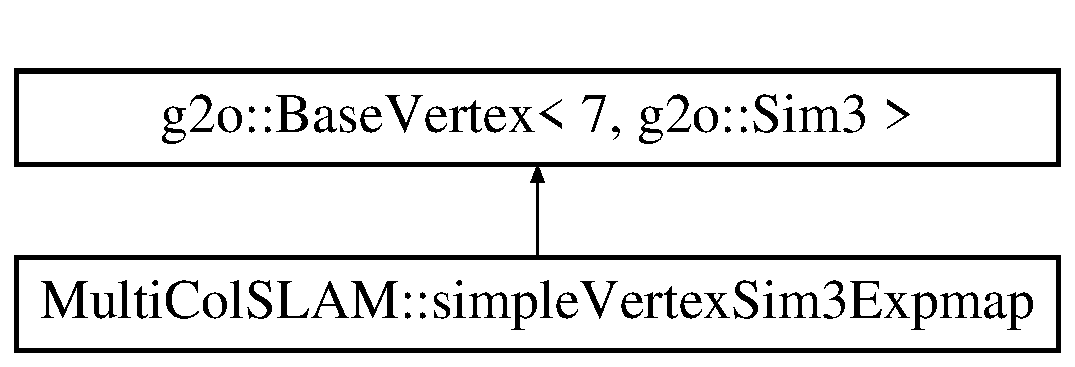
\includegraphics[height=2.000000cm]{classMultiColSLAM_1_1simpleVertexSim3Expmap}
\end{center}
\end{figure}
\subsection*{Public Member Functions}
\begin{DoxyCompactItemize}
\item 
virtual bool {\bfseries read} (std\+::istream \&is)\hypertarget{classMultiColSLAM_1_1simpleVertexSim3Expmap_a3aff42bc51c930ab46c597dbc1a27f17}{}\label{classMultiColSLAM_1_1simpleVertexSim3Expmap_a3aff42bc51c930ab46c597dbc1a27f17}

\item 
virtual bool {\bfseries write} (std\+::ostream \&os) const \hypertarget{classMultiColSLAM_1_1simpleVertexSim3Expmap_abb9068ae32fa75b2deebd35702b800ce}{}\label{classMultiColSLAM_1_1simpleVertexSim3Expmap_abb9068ae32fa75b2deebd35702b800ce}

\item 
virtual void {\bfseries set\+To\+Origin\+Impl} ()\hypertarget{classMultiColSLAM_1_1simpleVertexSim3Expmap_a1f2228bd267ebb9b47d21f981fcb6101}{}\label{classMultiColSLAM_1_1simpleVertexSim3Expmap_a1f2228bd267ebb9b47d21f981fcb6101}

\item 
virtual void {\bfseries oplus\+Impl} (const double $\ast$update\+\_\+)\hypertarget{classMultiColSLAM_1_1simpleVertexSim3Expmap_aaa78cb919385479caf5e1face579e0a3}{}\label{classMultiColSLAM_1_1simpleVertexSim3Expmap_aaa78cb919385479caf5e1face579e0a3}

\end{DoxyCompactItemize}
\subsection*{Public Attributes}
\begin{DoxyCompactItemize}
\item 
bool {\bfseries \+\_\+fix\+\_\+scale}\hypertarget{classMultiColSLAM_1_1simpleVertexSim3Expmap_a65cc7cb2c48a005c590ffe30794511f7}{}\label{classMultiColSLAM_1_1simpleVertexSim3Expmap_a65cc7cb2c48a005c590ffe30794511f7}

\end{DoxyCompactItemize}


\subsection{Detailed Description}
Sim3 Vertex, (x,y,z,qw,qx,qy,qz) the parameterization for the increments constructed is a 7d vector (x,y,z,qx,qy,qz) (note that we leave out the w part of the quaternion. 

The documentation for this class was generated from the following file\+:\begin{DoxyCompactItemize}
\item 
include/g2o\+\_\+\+Multi\+Col\+\_\+sim3\+\_\+expmap.\+h\end{DoxyCompactItemize}

\hypertarget{classMultiColSLAM_1_1VertexMc__cayley}{}\section{Multi\+Col\+S\+L\+AM\+:\+:Vertex\+Mc\+\_\+cayley Class Reference}
\label{classMultiColSLAM_1_1VertexMc__cayley}\index{Multi\+Col\+S\+L\+A\+M\+::\+Vertex\+Mc\+\_\+cayley@{Multi\+Col\+S\+L\+A\+M\+::\+Vertex\+Mc\+\_\+cayley}}
Inheritance diagram for Multi\+Col\+S\+L\+AM\+:\+:Vertex\+Mc\+\_\+cayley\+:\begin{figure}[H]
\begin{center}
\leavevmode
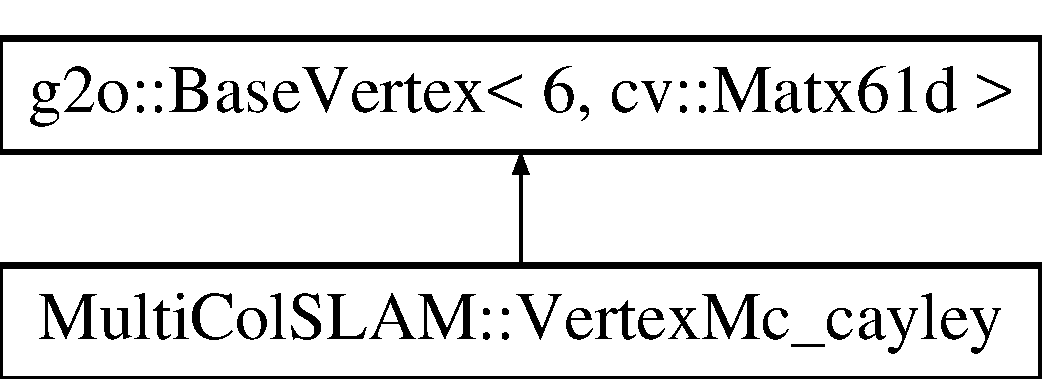
\includegraphics[height=2.000000cm]{classMultiColSLAM_1_1VertexMc__cayley}
\end{center}
\end{figure}
\subsection*{Public Member Functions}
\begin{DoxyCompactItemize}
\item 
virtual void {\bfseries set\+To\+Origin\+Impl} ()\hypertarget{classMultiColSLAM_1_1VertexMc__cayley_a3f176c92601fda3bed3fc9d6e586d9eb}{}\label{classMultiColSLAM_1_1VertexMc__cayley_a3f176c92601fda3bed3fc9d6e586d9eb}

\item 
virtual void {\bfseries oplus\+Impl} (const double $\ast$update\+\_\+)\hypertarget{classMultiColSLAM_1_1VertexMc__cayley_a897371c61e666db70c1d761d602efc6b}{}\label{classMultiColSLAM_1_1VertexMc__cayley_a897371c61e666db70c1d761d602efc6b}

\item 
bool {\bfseries read} (std\+::istream \&is)\hypertarget{classMultiColSLAM_1_1VertexMc__cayley_a9d3aca703f92f2728de5819872e5511d}{}\label{classMultiColSLAM_1_1VertexMc__cayley_a9d3aca703f92f2728de5819872e5511d}

\item 
bool {\bfseries write} (std\+::ostream \&os) const \hypertarget{classMultiColSLAM_1_1VertexMc__cayley_af24876878d2999276631d931cdeeb100}{}\label{classMultiColSLAM_1_1VertexMc__cayley_af24876878d2999276631d931cdeeb100}

\end{DoxyCompactItemize}


The documentation for this class was generated from the following file\+:\begin{DoxyCompactItemize}
\item 
include/g2o\+\_\+\+Multi\+Col\+\_\+vertices\+\_\+edges.\+h\end{DoxyCompactItemize}

\hypertarget{classMultiColSLAM_1_1VertexMt__cayley}{}\section{Multi\+Col\+S\+L\+AM\+:\+:Vertex\+Mt\+\_\+cayley Class Reference}
\label{classMultiColSLAM_1_1VertexMt__cayley}\index{Multi\+Col\+S\+L\+A\+M\+::\+Vertex\+Mt\+\_\+cayley@{Multi\+Col\+S\+L\+A\+M\+::\+Vertex\+Mt\+\_\+cayley}}
Inheritance diagram for Multi\+Col\+S\+L\+AM\+:\+:Vertex\+Mt\+\_\+cayley\+:\begin{figure}[H]
\begin{center}
\leavevmode
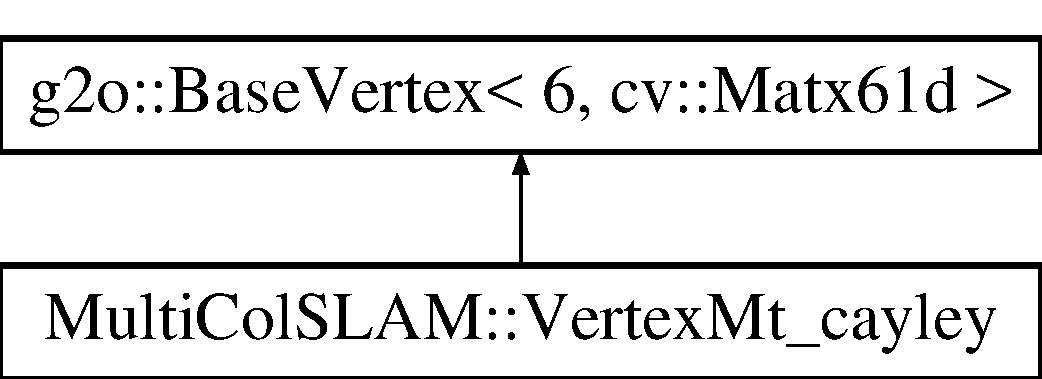
\includegraphics[height=2.000000cm]{classMultiColSLAM_1_1VertexMt__cayley}
\end{center}
\end{figure}
\subsection*{Public Member Functions}
\begin{DoxyCompactItemize}
\item 
virtual void {\bfseries set\+To\+Origin\+Impl} ()\hypertarget{classMultiColSLAM_1_1VertexMt__cayley_adfc6b70e21a0022fd4f76f2c4099bfd3}{}\label{classMultiColSLAM_1_1VertexMt__cayley_adfc6b70e21a0022fd4f76f2c4099bfd3}

\item 
virtual void {\bfseries oplus\+Impl} (const double $\ast$update\+\_\+)\hypertarget{classMultiColSLAM_1_1VertexMt__cayley_ad08baaa001240d2725c61463b185143f}{}\label{classMultiColSLAM_1_1VertexMt__cayley_ad08baaa001240d2725c61463b185143f}

\item 
bool {\bfseries read} (std\+::istream \&is)\hypertarget{classMultiColSLAM_1_1VertexMt__cayley_a9c30f22a6ed3382a46ea539aabd12cc8}{}\label{classMultiColSLAM_1_1VertexMt__cayley_a9c30f22a6ed3382a46ea539aabd12cc8}

\item 
bool {\bfseries write} (std\+::ostream \&os) const \hypertarget{classMultiColSLAM_1_1VertexMt__cayley_a68cf1a02055373cf62d42304b70e8acb}{}\label{classMultiColSLAM_1_1VertexMt__cayley_a68cf1a02055373cf62d42304b70e8acb}

\end{DoxyCompactItemize}


The documentation for this class was generated from the following file\+:\begin{DoxyCompactItemize}
\item 
include/g2o\+\_\+\+Multi\+Col\+\_\+vertices\+\_\+edges.\+h\end{DoxyCompactItemize}

\hypertarget{classMultiColSLAM_1_1VertexOmniCameraParameters}{}\section{Multi\+Col\+S\+L\+AM\+:\+:Vertex\+Omni\+Camera\+Parameters Class Reference}
\label{classMultiColSLAM_1_1VertexOmniCameraParameters}\index{Multi\+Col\+S\+L\+A\+M\+::\+Vertex\+Omni\+Camera\+Parameters@{Multi\+Col\+S\+L\+A\+M\+::\+Vertex\+Omni\+Camera\+Parameters}}
Inheritance diagram for Multi\+Col\+S\+L\+AM\+:\+:Vertex\+Omni\+Camera\+Parameters\+:\begin{figure}[H]
\begin{center}
\leavevmode
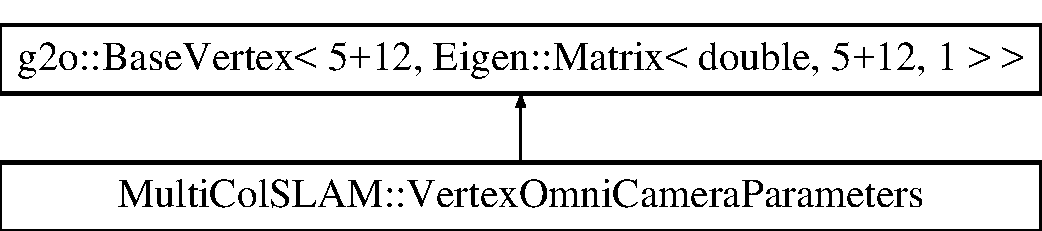
\includegraphics[height=2.000000cm]{classMultiColSLAM_1_1VertexOmniCameraParameters}
\end{center}
\end{figure}
\subsection*{Public Member Functions}
\begin{DoxyCompactItemize}
\item 
{\bfseries Vertex\+Omni\+Camera\+Parameters} (\hyperlink{classMultiColSLAM_1_1cCamModelGeneral__}{c\+Cam\+Model\+General\+\_\+} cam\+Model\+\_\+)\hypertarget{classMultiColSLAM_1_1VertexOmniCameraParameters_a2e4df6c0e7e4b51ba79f5e166313c5e1}{}\label{classMultiColSLAM_1_1VertexOmniCameraParameters_a2e4df6c0e7e4b51ba79f5e166313c5e1}

\item 
virtual void {\bfseries set\+To\+Origin\+Impl} ()\hypertarget{classMultiColSLAM_1_1VertexOmniCameraParameters_a8a126f0ab5b2e6a9c693d19296614372}{}\label{classMultiColSLAM_1_1VertexOmniCameraParameters_a8a126f0ab5b2e6a9c693d19296614372}

\item 
virtual void {\bfseries oplus\+Impl} (const double $\ast$update\+\_\+)\hypertarget{classMultiColSLAM_1_1VertexOmniCameraParameters_a60f0efd28a7113d1b5e9942a35edb78e}{}\label{classMultiColSLAM_1_1VertexOmniCameraParameters_a60f0efd28a7113d1b5e9942a35edb78e}

\item 
bool {\bfseries read} (std\+::istream \&is)\hypertarget{classMultiColSLAM_1_1VertexOmniCameraParameters_a2be61ec77f8a6bcb88e34d586a97c1e9}{}\label{classMultiColSLAM_1_1VertexOmniCameraParameters_a2be61ec77f8a6bcb88e34d586a97c1e9}

\item 
bool {\bfseries write} (std\+::ostream \&os) const \hypertarget{classMultiColSLAM_1_1VertexOmniCameraParameters_ae9f5bbe1ed20c05a40f01cee7e598a66}{}\label{classMultiColSLAM_1_1VertexOmniCameraParameters_ae9f5bbe1ed20c05a40f01cee7e598a66}

\end{DoxyCompactItemize}
\subsection*{Public Attributes}
\begin{DoxyCompactItemize}
\item 
{\bfseries E\+I\+G\+E\+N\+\_\+\+M\+A\+K\+E\+\_\+\+A\+L\+I\+G\+N\+E\+D\+\_\+\+O\+P\+E\+R\+A\+T\+O\+R\+\_\+\+N\+EW}\hypertarget{classMultiColSLAM_1_1VertexOmniCameraParameters_a2bfa28f2c03ee89f1a1a44e62787b5f5}{}\label{classMultiColSLAM_1_1VertexOmniCameraParameters_a2bfa28f2c03ee89f1a1a44e62787b5f5}

\item 
\hyperlink{classMultiColSLAM_1_1cCamModelGeneral__}{c\+Cam\+Model\+General\+\_\+} {\bfseries cam\+Model}\hypertarget{classMultiColSLAM_1_1VertexOmniCameraParameters_af64ebab6fa8ce6e44e8e09a737d11571}{}\label{classMultiColSLAM_1_1VertexOmniCameraParameters_af64ebab6fa8ce6e44e8e09a737d11571}

\end{DoxyCompactItemize}


The documentation for this class was generated from the following file\+:\begin{DoxyCompactItemize}
\item 
include/g2o\+\_\+\+Multi\+Col\+\_\+vertices\+\_\+edges.\+h\end{DoxyCompactItemize}

\hypertarget{classMultiColSLAM_1_1VertexPointXYZ}{}\section{Multi\+Col\+S\+L\+AM\+:\+:Vertex\+Point\+X\+YZ Class Reference}
\label{classMultiColSLAM_1_1VertexPointXYZ}\index{Multi\+Col\+S\+L\+A\+M\+::\+Vertex\+Point\+X\+YZ@{Multi\+Col\+S\+L\+A\+M\+::\+Vertex\+Point\+X\+YZ}}


Point vertex, X\+YZ.  




{\ttfamily \#include $<$g2o\+\_\+\+Multi\+Col\+\_\+vertices\+\_\+edges.\+h$>$}

Inheritance diagram for Multi\+Col\+S\+L\+AM\+:\+:Vertex\+Point\+X\+YZ\+:\begin{figure}[H]
\begin{center}
\leavevmode
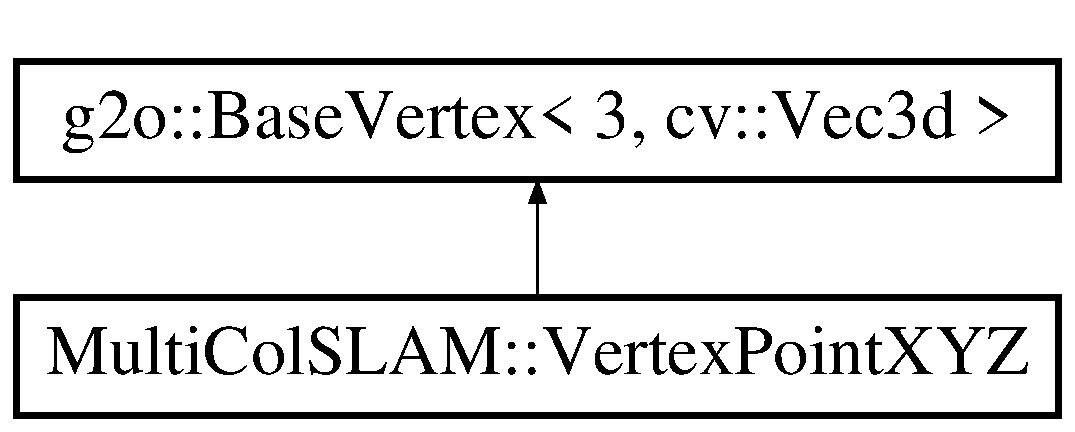
\includegraphics[height=2.000000cm]{classMultiColSLAM_1_1VertexPointXYZ}
\end{center}
\end{figure}
\subsection*{Public Member Functions}
\begin{DoxyCompactItemize}
\item 
virtual void {\bfseries set\+To\+Origin\+Impl} ()\hypertarget{classMultiColSLAM_1_1VertexPointXYZ_a9557cd0e17b562bb172908d03546cafd}{}\label{classMultiColSLAM_1_1VertexPointXYZ_a9557cd0e17b562bb172908d03546cafd}

\item 
virtual void {\bfseries oplus\+Impl} (const double $\ast$update)\hypertarget{classMultiColSLAM_1_1VertexPointXYZ_a36702c3d044af4dcf713bb428a35b866}{}\label{classMultiColSLAM_1_1VertexPointXYZ_a36702c3d044af4dcf713bb428a35b866}

\item 
virtual bool {\bfseries read} (std\+::istream \&)\hypertarget{classMultiColSLAM_1_1VertexPointXYZ_afe359248a103b4908bd6c0e6a6bc0f41}{}\label{classMultiColSLAM_1_1VertexPointXYZ_afe359248a103b4908bd6c0e6a6bc0f41}

\item 
virtual bool {\bfseries write} (std\+::ostream \&) const \hypertarget{classMultiColSLAM_1_1VertexPointXYZ_ad6bc53b4c5950ca6495a75753b618498}{}\label{classMultiColSLAM_1_1VertexPointXYZ_ad6bc53b4c5950ca6495a75753b618498}

\item 
void {\bfseries Set\+ID} (int id)\hypertarget{classMultiColSLAM_1_1VertexPointXYZ_a8d08fcbfb1327472eba01ab3e40caaa4}{}\label{classMultiColSLAM_1_1VertexPointXYZ_a8d08fcbfb1327472eba01ab3e40caaa4}

\item 
int {\bfseries Get\+ID} ()\hypertarget{classMultiColSLAM_1_1VertexPointXYZ_afc60be4d7a2318d72813a296ddb6d740}{}\label{classMultiColSLAM_1_1VertexPointXYZ_afc60be4d7a2318d72813a296ddb6d740}

\end{DoxyCompactItemize}
\subsection*{Public Attributes}
\begin{DoxyCompactItemize}
\item 
int {\bfseries pt\+ID}\hypertarget{classMultiColSLAM_1_1VertexPointXYZ_aa8483e9fe70fa64e8cb0c9464344bf4c}{}\label{classMultiColSLAM_1_1VertexPointXYZ_aa8483e9fe70fa64e8cb0c9464344bf4c}

\end{DoxyCompactItemize}


\subsection{Detailed Description}
Point vertex, X\+YZ. 

The documentation for this class was generated from the following file\+:\begin{DoxyCompactItemize}
\item 
include/g2o\+\_\+\+Multi\+Col\+\_\+vertices\+\_\+edges.\+h\end{DoxyCompactItemize}

\hypertarget{classMultiColSLAM_1_1VertexSim3Expmap__Multi}{}\section{Multi\+Col\+S\+L\+AM\+:\+:Vertex\+Sim3\+Expmap\+\_\+\+Multi Class Reference}
\label{classMultiColSLAM_1_1VertexSim3Expmap__Multi}\index{Multi\+Col\+S\+L\+A\+M\+::\+Vertex\+Sim3\+Expmap\+\_\+\+Multi@{Multi\+Col\+S\+L\+A\+M\+::\+Vertex\+Sim3\+Expmap\+\_\+\+Multi}}
Inheritance diagram for Multi\+Col\+S\+L\+AM\+:\+:Vertex\+Sim3\+Expmap\+\_\+\+Multi\+:\begin{figure}[H]
\begin{center}
\leavevmode
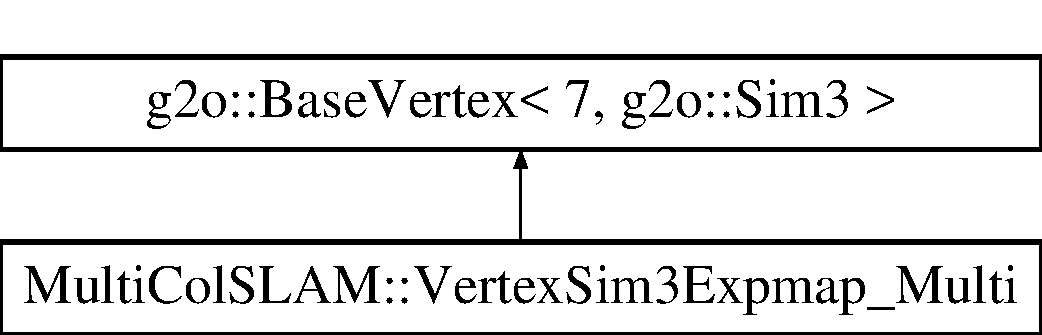
\includegraphics[height=2.000000cm]{classMultiColSLAM_1_1VertexSim3Expmap__Multi}
\end{center}
\end{figure}
\subsection*{Public Member Functions}
\begin{DoxyCompactItemize}
\item 
{\bfseries Vertex\+Sim3\+Expmap\+\_\+\+Multi} (std\+::unordered\+\_\+map$<$ size\+\_\+t, int $>$ \&kp\+\_\+to\+\_\+cam1, std\+::unordered\+\_\+map$<$ size\+\_\+t, int $>$ \&kp\+\_\+to\+\_\+cam2)\hypertarget{classMultiColSLAM_1_1VertexSim3Expmap__Multi_add103ed89904b987a14b9c5257a2002f}{}\label{classMultiColSLAM_1_1VertexSim3Expmap__Multi_add103ed89904b987a14b9c5257a2002f}

\item 
virtual void {\bfseries set\+To\+Origin\+Impl} ()\hypertarget{classMultiColSLAM_1_1VertexSim3Expmap__Multi_a20483aef66ae48d312190b3eebea3670}{}\label{classMultiColSLAM_1_1VertexSim3Expmap__Multi_a20483aef66ae48d312190b3eebea3670}

\item 
virtual void {\bfseries oplus\+Impl} (const double $\ast$update\+\_\+)\hypertarget{classMultiColSLAM_1_1VertexSim3Expmap__Multi_aefd1904bc6ee3641e77c179fb4ca95cc}{}\label{classMultiColSLAM_1_1VertexSim3Expmap__Multi_aefd1904bc6ee3641e77c179fb4ca95cc}

\item 
cv\+::\+Vec2d {\bfseries cam\+\_\+map1} (const Eigen\+::\+Vector3d \&v, int pt\+Idx) const \hypertarget{classMultiColSLAM_1_1VertexSim3Expmap__Multi_a7841d1f192b0930af6a988c909dc5d40}{}\label{classMultiColSLAM_1_1VertexSim3Expmap__Multi_a7841d1f192b0930af6a988c909dc5d40}

\item 
cv\+::\+Vec2d {\bfseries cam\+\_\+map2} (const Eigen\+::\+Vector3d \&v, int pt\+Idx) const \hypertarget{classMultiColSLAM_1_1VertexSim3Expmap__Multi_acf01b0f19b5e72e0eb9fd8e0f8b24431}{}\label{classMultiColSLAM_1_1VertexSim3Expmap__Multi_acf01b0f19b5e72e0eb9fd8e0f8b24431}

\item 
bool {\bfseries read} (std\+::istream \&is)\hypertarget{classMultiColSLAM_1_1VertexSim3Expmap__Multi_a45ce305be328622b172e302f6d758988}{}\label{classMultiColSLAM_1_1VertexSim3Expmap__Multi_a45ce305be328622b172e302f6d758988}

\item 
bool {\bfseries write} (std\+::ostream \&os) const \hypertarget{classMultiColSLAM_1_1VertexSim3Expmap__Multi_a3ecf0aa5d0f7465e96f7b6cfd51ad6d8}{}\label{classMultiColSLAM_1_1VertexSim3Expmap__Multi_a3ecf0aa5d0f7465e96f7b6cfd51ad6d8}

\end{DoxyCompactItemize}
\subsection*{Public Attributes}
\begin{DoxyCompactItemize}
\item 
\hyperlink{classMultiColSLAM_1_1cMultiCamSys__}{c\+Multi\+Cam\+Sys\+\_\+} $\ast$ {\bfseries cam\+Sys1}\hypertarget{classMultiColSLAM_1_1VertexSim3Expmap__Multi_a6f0f67d20c6a54551e84c7dfc9b12e97}{}\label{classMultiColSLAM_1_1VertexSim3Expmap__Multi_a6f0f67d20c6a54551e84c7dfc9b12e97}

\item 
\hyperlink{classMultiColSLAM_1_1cMultiCamSys__}{c\+Multi\+Cam\+Sys\+\_\+} $\ast$ {\bfseries cam\+Sys2}\hypertarget{classMultiColSLAM_1_1VertexSim3Expmap__Multi_a16032c67f53b74c97969a97b1c207587}{}\label{classMultiColSLAM_1_1VertexSim3Expmap__Multi_a16032c67f53b74c97969a97b1c207587}

\item 
bool {\bfseries \+\_\+fix\+\_\+scale}\hypertarget{classMultiColSLAM_1_1VertexSim3Expmap__Multi_a905badf8def1b61cace42846b91a88a2}{}\label{classMultiColSLAM_1_1VertexSim3Expmap__Multi_a905badf8def1b61cace42846b91a88a2}

\item 
std\+::unordered\+\_\+map$<$ size\+\_\+t, int $>$ {\bfseries keypoint\+\_\+to\+\_\+cam1}\hypertarget{classMultiColSLAM_1_1VertexSim3Expmap__Multi_aaec9c7acb3643544e68e1540b7d079b0}{}\label{classMultiColSLAM_1_1VertexSim3Expmap__Multi_aaec9c7acb3643544e68e1540b7d079b0}

\item 
std\+::unordered\+\_\+map$<$ size\+\_\+t, int $>$ {\bfseries keypoint\+\_\+to\+\_\+cam2}\hypertarget{classMultiColSLAM_1_1VertexSim3Expmap__Multi_a6ef1ee9d62791dd19bb653c41d3eeb65}{}\label{classMultiColSLAM_1_1VertexSim3Expmap__Multi_a6ef1ee9d62791dd19bb653c41d3eeb65}

\end{DoxyCompactItemize}


The documentation for this class was generated from the following file\+:\begin{DoxyCompactItemize}
\item 
include/g2o\+\_\+\+Multi\+Col\+\_\+sim3\+\_\+expmap.\+h\end{DoxyCompactItemize}

%--- End generated contents ---

% Index
\backmatter
\newpage
\phantomsection
\clearemptydoublepage
\addcontentsline{toc}{chapter}{Index}
\printindex

\end{document}
